\documentclass[a4paper]{book}
\usepackage{makeidx}
\usepackage{natbib}
\usepackage{graphicx}
\usepackage{multicol}
\usepackage{float}
\usepackage{listings}
\usepackage{color}
\usepackage{ifthen}
\usepackage[table]{xcolor}
\usepackage{textcomp}
\usepackage{alltt}
\usepackage{ifpdf}
\ifpdf
\usepackage[pdftex,
            pagebackref=true,
            colorlinks=true,
            linkcolor=blue,
            unicode
           ]{hyperref}
\else
\usepackage[ps2pdf,
            pagebackref=true,
            colorlinks=true,
            linkcolor=blue,
            unicode
           ]{hyperref}
\usepackage{pspicture}
\fi
\usepackage[utf8]{inputenc}
\usepackage{mathptmx}
\usepackage[scaled=.90]{helvet}
\usepackage{courier}
\usepackage{sectsty}
\usepackage[titles]{tocloft}
\usepackage{doxygen}
\lstset{language=C++,inputencoding=utf8,basicstyle=\footnotesize,breaklines=true,breakatwhitespace=true,tabsize=8,numbers=left }
\makeindex
\setcounter{tocdepth}{3}
\renewcommand{\footrulewidth}{0.4pt}
\renewcommand{\familydefault}{\sfdefault}
\hfuzz=15pt
\setlength{\emergencystretch}{15pt}
\hbadness=750
\tolerance=750
\begin{document}
\hypersetup{pageanchor=false,citecolor=blue}
\begin{titlepage}
\vspace*{7cm}
\begin{center}
{\Large \-F\-I\-R\-M-\/\-O\-M\-P\-L }\\
\vspace*{1cm}
{\large \-Generated by Doxygen 1.7.6.1}\\
\vspace*{0.5cm}
{\small Wed Mar 26 2014 20:46:56}\\
\end{center}
\end{titlepage}
\clearemptydoublepage
\pagenumbering{roman}
\tableofcontents
\clearemptydoublepage
\pagenumbering{arabic}
\hypersetup{pageanchor=true,citecolor=blue}
\chapter{\-Deprecated \-List}
\label{deprecated}
\hypertarget{deprecated}{}

\begin{DoxyRefList}
\item[\label{deprecated__deprecated000002}%
\hypertarget{deprecated__deprecated000002}{}%
\-Member \hyperlink{class_ti_xml_handle_acb5fe8388a526289ea65e817a51e05e7}{\-Ti\-Xml\-Handle\-:\-:\-Element} () const ]use \-To\-Element. \-Return the handle as a \hyperlink{class_ti_xml_element}{\-Ti\-Xml\-Element}. \-This may return null.  
\item[\label{deprecated__deprecated000001}%
\hypertarget{deprecated__deprecated000001}{}%
\-Member \hyperlink{class_ti_xml_handle_ab44b723a8dc9af72838a303c079d0376}{\-Ti\-Xml\-Handle\-:\-:\-Node} () const ]use \-To\-Node. \-Return the handle as a \hyperlink{class_ti_xml_node}{\-Ti\-Xml\-Node}. \-This may return null.  
\item[\label{deprecated__deprecated000003}%
\hypertarget{deprecated__deprecated000003}{}%
\-Member \hyperlink{class_ti_xml_handle_a9fc739c8a18d160006f82572fc143d13}{\-Ti\-Xml\-Handle\-:\-:\-Text} () const ]use \-To\-Text() \-Return the handle as a \hyperlink{class_ti_xml_text}{\-Ti\-Xml\-Text}. \-This may return null.  
\item[\label{deprecated__deprecated000004}%
\hypertarget{deprecated__deprecated000004}{}%
\-Member \hyperlink{class_ti_xml_handle_a49675b74357ba2aae124657a9a1ef465}{\-Ti\-Xml\-Handle\-:\-:\-Unknown} () const ]use \-To\-Unknown() \-Return the handle as a \hyperlink{class_ti_xml_unknown}{\-Ti\-Xml\-Unknown}. \-This may return null. 
\end{DoxyRefList}
\chapter{\-Namespace \-Index}
\section{\-Namespace \-List}
\-Here is a list of all documented namespaces with brief descriptions\-:\begin{DoxyCompactList}
\item\contentsline{section}{\hyperlink{namespacefirm}{firm} }{\pageref{namespacefirm}}{}
\end{DoxyCompactList}

\chapter{\-Class \-Index}
\section{\-Class \-Hierarchy}
\-This inheritance list is sorted roughly, but not completely, alphabetically\-:\begin{DoxyCompactList}
\item \contentsline{section}{\-Actuation\-System\-Method}{\pageref{class_actuation_system_method}}{}
\begin{DoxyCompactList}
\item \contentsline{section}{\-Simulated\-Actuation\-System}{\pageref{class_simulated_actuation_system}}{}
\end{DoxyCompactList}
\item \contentsline{section}{\-Controller$<$ \-Separated\-Controller\-Type, \-Filter\-Type $>$}{\pageref{class_controller}}{}
\item \contentsline{section}{\-Double\-Value\-Comp}{\pageref{struct_double_value_comp}}{}
\item \contentsline{section}{\-F\-I\-R\-M\-:\-:edge\-\_\-flags\-\_\-t}{\pageref{struct_f_i_r_m_1_1edge__flags__t}}{}
\item \contentsline{section}{\-Edge\-Comp}{\pageref{struct_edge_comp}}{}
\item \contentsline{section}{\-Feedback\-Path}{\pageref{class_feedback_path}}{}
\item \contentsline{section}{\-F\-I\-R\-M}{\pageref{class_f_i_r_m}}{}
\item \contentsline{section}{\-F\-I\-R\-M\-Optimization\-Objective}{\pageref{class_f_i_r_m_optimization_objective}}{}
\item \contentsline{section}{\-F\-I\-R\-M\-Validity\-Checker}{\pageref{class_f_i_r_m_validity_checker}}{}
\item \contentsline{section}{\-F\-I\-R\-M\-Weight}{\pageref{class_f_i_r_m_weight}}{}
\item \contentsline{section}{\-Gaussian\-Valid\-Belief\-Sampler}{\pageref{class_gaussian_valid_belief_sampler}}{}
\item \contentsline{section}{\-Kalman\-Filter\-Method}{\pageref{class_kalman_filter_method}}{}
\begin{DoxyCompactList}
\item \contentsline{section}{\-Extended\-K\-F}{\pageref{class_extended_k_f}}{}
\item \contentsline{section}{\-Linearized\-K\-F}{\pageref{class_linearized_k_f}}{}
\end{DoxyCompactList}
\item \contentsline{section}{\-Linear\-System}{\pageref{class_linear_system}}{}
\item \contentsline{section}{\-Motion\-Model\-Method}{\pageref{class_motion_model_method}}{}
\begin{DoxyCompactList}
\item \contentsline{section}{\-Unicycle\-Motion\-Model}{\pageref{class_unicycle_motion_model}}{}
\end{DoxyCompactList}
\item \contentsline{section}{\-Observation\-Model\-Method}{\pageref{class_observation_model_method}}{}
\begin{DoxyCompactList}
\item \contentsline{section}{\-Cam\-Aruco2\-D\-Observation\-Model}{\pageref{class_cam_aruco2_d_observation_model}}{}
\end{DoxyCompactList}
\item \contentsline{section}{\-S\-E2\-Belief\-Space}{\pageref{class_s_e2_belief_space}}{}
\item \contentsline{section}{\-Separated\-Controller\-Method}{\pageref{class_separated_controller_method}}{}
\begin{DoxyCompactList}
\item \contentsline{section}{\-R\-H\-C\-I\-Create}{\pageref{class_r_h_c_i_create}}{}
\end{DoxyCompactList}
\item \contentsline{section}{firm\-:\-:\-Space\-Information}{\pageref{classfirm_1_1_space_information}}{}
\item \contentsline{section}{\-S\-E2\-Belief\-Space\-:\-:\-State\-Type}{\pageref{class_s_e2_belief_space_1_1_state_type}}{}
\item \contentsline{section}{\-Ti\-Xml\-Attribute\-Set}{\pageref{class_ti_xml_attribute_set}}{}
\item \contentsline{section}{\-Ti\-Xml\-Base}{\pageref{class_ti_xml_base}}{}
\begin{DoxyCompactList}
\item \contentsline{section}{\-Ti\-Xml\-Attribute}{\pageref{class_ti_xml_attribute}}{}
\item \contentsline{section}{\-Ti\-Xml\-Node}{\pageref{class_ti_xml_node}}{}
\begin{DoxyCompactList}
\item \contentsline{section}{\-Ti\-Xml\-Comment}{\pageref{class_ti_xml_comment}}{}
\item \contentsline{section}{\-Ti\-Xml\-Declaration}{\pageref{class_ti_xml_declaration}}{}
\item \contentsline{section}{\-Ti\-Xml\-Document}{\pageref{class_ti_xml_document}}{}
\item \contentsline{section}{\-Ti\-Xml\-Element}{\pageref{class_ti_xml_element}}{}
\item \contentsline{section}{\-Ti\-Xml\-Text}{\pageref{class_ti_xml_text}}{}
\item \contentsline{section}{\-Ti\-Xml\-Unknown}{\pageref{class_ti_xml_unknown}}{}
\end{DoxyCompactList}
\end{DoxyCompactList}
\item \contentsline{section}{\-Ti\-Xml\-Cursor}{\pageref{struct_ti_xml_cursor}}{}
\item \contentsline{section}{\-Ti\-Xml\-Handle}{\pageref{class_ti_xml_handle}}{}
\item \contentsline{section}{\-Ti\-Xml\-Parsing\-Data}{\pageref{class_ti_xml_parsing_data}}{}
\item \contentsline{section}{\-Ti\-Xml\-String}{\pageref{class_ti_xml_string}}{}
\begin{DoxyCompactList}
\item \contentsline{section}{\-Ti\-Xml\-Out\-Stream}{\pageref{class_ti_xml_out_stream}}{}
\end{DoxyCompactList}
\item \contentsline{section}{\-Ti\-Xml\-Visitor}{\pageref{class_ti_xml_visitor}}{}
\begin{DoxyCompactList}
\item \contentsline{section}{\-Ti\-Xml\-Printer}{\pageref{class_ti_xml_printer}}{}
\end{DoxyCompactList}
\item \contentsline{section}{\-Unicycle\-State\-Propagator}{\pageref{class_unicycle_state_propagator}}{}
\item \contentsline{section}{\-Uniform\-Valid\-Belief\-Sampler}{\pageref{class_uniform_valid_belief_sampler}}{}
\item \contentsline{section}{\-F\-I\-R\-M\-:\-:vertex\-\_\-flags\-\_\-t}{\pageref{struct_f_i_r_m_1_1vertex__flags__t}}{}
\item \contentsline{section}{\-F\-I\-R\-M\-:\-:vertex\-\_\-state\-\_\-t}{\pageref{struct_f_i_r_m_1_1vertex__state__t}}{}
\item \contentsline{section}{\-F\-I\-R\-M\-:\-:vertex\-\_\-successful\-\_\-connection\-\_\-attempts\-\_\-t}{\pageref{struct_f_i_r_m_1_1vertex__successful__connection__attempts__t}}{}
\item \contentsline{section}{\-F\-I\-R\-M\-:\-:vertex\-\_\-total\-\_\-connection\-\_\-attempts\-\_\-t}{\pageref{struct_f_i_r_m_1_1vertex__total__connection__attempts__t}}{}
\end{DoxyCompactList}

\chapter{\-Class \-Index}
\section{\-Class \-List}
\-Here are the classes, structs, unions and interfaces with brief descriptions\-:\begin{DoxyCompactList}
\item\contentsline{section}{\hyperlink{class_actuation_system_method}{\-Actuation\-System\-Method} }{\pageref{class_actuation_system_method}}{}
\item\contentsline{section}{\hyperlink{class_cam_aruco2_d_observation_model}{\-Cam\-Aruco2\-D\-Observation\-Model} }{\pageref{class_cam_aruco2_d_observation_model}}{}
\item\contentsline{section}{\hyperlink{class_controller}{\-Controller$<$ Separated\-Controller\-Type, Filter\-Type $>$} \\*\-Base class for \hyperlink{class_controller}{\-Controller}. \-A controller's task is to use the filter to estimate the belief robot's state and generate control commands using the separated controller. \-For example by fusing an \-L\-Q\-R and \-Kalman \-Filter we generate an \-L\-Q\-G controller }{\pageref{class_controller}}{}
\item\contentsline{section}{\hyperlink{struct_double_value_comp}{\-Double\-Value\-Comp} }{\pageref{struct_double_value_comp}}{}
\item\contentsline{section}{\hyperlink{struct_f_i_r_m_1_1edge__flags__t}{\-F\-I\-R\-M\-::edge\-\_\-flags\-\_\-t} }{\pageref{struct_f_i_r_m_1_1edge__flags__t}}{}
\item\contentsline{section}{\hyperlink{struct_edge_comp}{\-Edge\-Comp} }{\pageref{struct_edge_comp}}{}
\item\contentsline{section}{\hyperlink{struct_ti_xml_base_1_1_entity}{\-Ti\-Xml\-Base\-::\-Entity} }{\pageref{struct_ti_xml_base_1_1_entity}}{}
\item\contentsline{section}{\hyperlink{class_extended_k_f}{\-Extended\-K\-F} }{\pageref{class_extended_k_f}}{}
\item\contentsline{section}{\hyperlink{class_feedback_path}{\-Feedback\-Path} }{\pageref{class_feedback_path}}{}
\item\contentsline{section}{\hyperlink{class_f_i_r_m}{\-F\-I\-R\-M} \\*\-Feedback \-Information \-Road\-Map planner }{\pageref{class_f_i_r_m}}{}
\item\contentsline{section}{\hyperlink{class_f_i_r_m_optimization_objective}{\-F\-I\-R\-M\-Optimization\-Objective} }{\pageref{class_f_i_r_m_optimization_objective}}{}
\item\contentsline{section}{\hyperlink{class_f_i_r_m_validity_checker}{\-F\-I\-R\-M\-Validity\-Checker} }{\pageref{class_f_i_r_m_validity_checker}}{}
\item\contentsline{section}{\hyperlink{class_f_i_r_m_weight}{\-F\-I\-R\-M\-Weight} }{\pageref{class_f_i_r_m_weight}}{}
\item\contentsline{section}{\hyperlink{class_f_strategy}{\-F\-Strategy$<$ Milestone $>$} }{\pageref{class_f_strategy}}{}
\item\contentsline{section}{\hyperlink{class_gaussian_valid_belief_sampler}{\-Gaussian\-Valid\-Belief\-Sampler} \\*\-Generate valid samples using the \-Gaussian sampling strategy }{\pageref{class_gaussian_valid_belief_sampler}}{}
\item\contentsline{section}{\hyperlink{class_g_l_widget}{\-G\-L\-Widget} }{\pageref{class_g_l_widget}}{}
\item\contentsline{section}{\hyperlink{class_kalman_filter_method}{\-Kalman\-Filter\-Method} }{\pageref{class_kalman_filter_method}}{}
\item\contentsline{section}{\hyperlink{class_linearized_k_f}{\-Linearized\-K\-F} }{\pageref{class_linearized_k_f}}{}
\item\contentsline{section}{\hyperlink{class_linear_system}{\-Linear\-System} }{\pageref{class_linear_system}}{}
\item\contentsline{section}{\hyperlink{class_motion_model_method}{\-Motion\-Model\-Method} }{\pageref{class_motion_model_method}}{}
\item\contentsline{section}{\hyperlink{class_my_window}{\-My\-Window} }{\pageref{class_my_window}}{}
\item\contentsline{section}{\hyperlink{class_observation_model_method}{\-Observation\-Model\-Method} }{\pageref{class_observation_model_method}}{}
\item\contentsline{section}{\hyperlink{class_o_g_l_display}{\-O\-G\-L\-Display} }{\pageref{class_o_g_l_display}}{}
\item\contentsline{section}{\hyperlink{struct_o_g_l_display_1_1_o_g_l_feedback_edge}{\-O\-G\-L\-Display\-::\-O\-G\-L\-Feedback\-Edge} }{\pageref{struct_o_g_l_display_1_1_o_g_l_feedback_edge}}{}
\item\contentsline{section}{\hyperlink{struct_ti_xml_string_1_1_rep}{\-Ti\-Xml\-String\-::\-Rep} }{\pageref{struct_ti_xml_string_1_1_rep}}{}
\item\contentsline{section}{\hyperlink{class_r_h_c_i_create}{\-R\-H\-C\-I\-Create} }{\pageref{class_r_h_c_i_create}}{}
\item\contentsline{section}{\hyperlink{class_s_e2_belief_space}{\-S\-E2\-Belief\-Space} }{\pageref{class_s_e2_belief_space}}{}
\item\contentsline{section}{\hyperlink{class_separated_controller_method}{\-Separated\-Controller\-Method} }{\pageref{class_separated_controller_method}}{}
\item\contentsline{section}{\hyperlink{class_simulated_actuation_system}{\-Simulated\-Actuation\-System} }{\pageref{class_simulated_actuation_system}}{}
\item\contentsline{section}{\hyperlink{classfirm_1_1_space_information}{firm\-::\-Space\-Information} }{\pageref{classfirm_1_1_space_information}}{}
\item\contentsline{section}{\hyperlink{class_s_e2_belief_space_1_1_state_type}{\-S\-E2\-Belief\-Space\-::\-State\-Type} \\*\-A belief in \-S\-E(2)\-: (x, y, yaw, covariance) }{\pageref{class_s_e2_belief_space_1_1_state_type}}{}
\item\contentsline{section}{\hyperlink{class_ti_xml_attribute}{\-Ti\-Xml\-Attribute} }{\pageref{class_ti_xml_attribute}}{}
\item\contentsline{section}{\hyperlink{class_ti_xml_attribute_set}{\-Ti\-Xml\-Attribute\-Set} }{\pageref{class_ti_xml_attribute_set}}{}
\item\contentsline{section}{\hyperlink{class_ti_xml_base}{\-Ti\-Xml\-Base} }{\pageref{class_ti_xml_base}}{}
\item\contentsline{section}{\hyperlink{class_ti_xml_comment}{\-Ti\-Xml\-Comment} }{\pageref{class_ti_xml_comment}}{}
\item\contentsline{section}{\hyperlink{struct_ti_xml_cursor}{\-Ti\-Xml\-Cursor} }{\pageref{struct_ti_xml_cursor}}{}
\item\contentsline{section}{\hyperlink{class_ti_xml_declaration}{\-Ti\-Xml\-Declaration} }{\pageref{class_ti_xml_declaration}}{}
\item\contentsline{section}{\hyperlink{class_ti_xml_document}{\-Ti\-Xml\-Document} }{\pageref{class_ti_xml_document}}{}
\item\contentsline{section}{\hyperlink{class_ti_xml_element}{\-Ti\-Xml\-Element} }{\pageref{class_ti_xml_element}}{}
\item\contentsline{section}{\hyperlink{class_ti_xml_handle}{\-Ti\-Xml\-Handle} }{\pageref{class_ti_xml_handle}}{}
\item\contentsline{section}{\hyperlink{class_ti_xml_node}{\-Ti\-Xml\-Node} }{\pageref{class_ti_xml_node}}{}
\item\contentsline{section}{\hyperlink{class_ti_xml_out_stream}{\-Ti\-Xml\-Out\-Stream} }{\pageref{class_ti_xml_out_stream}}{}
\item\contentsline{section}{\hyperlink{class_ti_xml_parsing_data}{\-Ti\-Xml\-Parsing\-Data} }{\pageref{class_ti_xml_parsing_data}}{}
\item\contentsline{section}{\hyperlink{class_ti_xml_printer}{\-Ti\-Xml\-Printer} }{\pageref{class_ti_xml_printer}}{}
\item\contentsline{section}{\hyperlink{class_ti_xml_string}{\-Ti\-Xml\-String} }{\pageref{class_ti_xml_string}}{}
\item\contentsline{section}{\hyperlink{class_ti_xml_text}{\-Ti\-Xml\-Text} }{\pageref{class_ti_xml_text}}{}
\item\contentsline{section}{\hyperlink{class_ti_xml_unknown}{\-Ti\-Xml\-Unknown} }{\pageref{class_ti_xml_unknown}}{}
\item\contentsline{section}{\hyperlink{class_ti_xml_visitor}{\-Ti\-Xml\-Visitor} }{\pageref{class_ti_xml_visitor}}{}
\item\contentsline{section}{\hyperlink{class_unicycle_motion_model}{\-Unicycle\-Motion\-Model} }{\pageref{class_unicycle_motion_model}}{}
\item\contentsline{section}{\hyperlink{class_unicycle_state_propagator}{\-Unicycle\-State\-Propagator} \\*\-State propagation for a unicycle motion model }{\pageref{class_unicycle_state_propagator}}{}
\item\contentsline{section}{\hyperlink{class_uniform_valid_belief_sampler}{\-Uniform\-Valid\-Belief\-Sampler} \\*\-Generate valid samples using the \-Uniform sampling strategy }{\pageref{class_uniform_valid_belief_sampler}}{}
\item\contentsline{section}{\hyperlink{struct_f_i_r_m_1_1vertex__flags__t}{\-F\-I\-R\-M\-::vertex\-\_\-flags\-\_\-t} }{\pageref{struct_f_i_r_m_1_1vertex__flags__t}}{}
\item\contentsline{section}{\hyperlink{struct_f_i_r_m_1_1vertex__state__t}{\-F\-I\-R\-M\-::vertex\-\_\-state\-\_\-t} }{\pageref{struct_f_i_r_m_1_1vertex__state__t}}{}
\item\contentsline{section}{\hyperlink{struct_f_i_r_m_1_1vertex__successful__connection__attempts__t}{\-F\-I\-R\-M\-::vertex\-\_\-successful\-\_\-connection\-\_\-attempts\-\_\-t} }{\pageref{struct_f_i_r_m_1_1vertex__successful__connection__attempts__t}}{}
\item\contentsline{section}{\hyperlink{struct_f_i_r_m_1_1vertex__total__connection__attempts__t}{\-F\-I\-R\-M\-::vertex\-\_\-total\-\_\-connection\-\_\-attempts\-\_\-t} }{\pageref{struct_f_i_r_m_1_1vertex__total__connection__attempts__t}}{}
\item\contentsline{section}{\hyperlink{class_visualizer}{\-Visualizer} }{\pageref{class_visualizer}}{}
\item\contentsline{section}{\hyperlink{struct_visualizer_1_1_v_z_r_feedback_edge}{\-Visualizer\-::\-V\-Z\-R\-Feedback\-Edge} }{\pageref{struct_visualizer_1_1_v_z_r_feedback_edge}}{}
\end{DoxyCompactList}

\chapter{\-Namespace \-Documentation}
\hypertarget{namespacefirm}{\section{firm \-Namespace \-Reference}
\label{namespacefirm}\index{firm@{firm}}
}
\subsection*{\-Classes}
\begin{DoxyCompactItemize}
\item 
class \hyperlink{classfirm_1_1_space_information}{\-Space\-Information}
\end{DoxyCompactItemize}


\subsection{\-Detailed \-Description}
\-The \-F\-I\-R\-M\-Space information class is a derivative of the control\-::spaceinformation that enables us to add \hyperlink{class_f_i_r_m}{\-F\-I\-R\-M} specific information to the space. \-Specifically, we need to use the motion/observation models time and again. \-We need not construct them multiple times. \-Instead, we can make them members of this new class 
\chapter{\-Class \-Documentation}
\hypertarget{class_actuation_system_method}{\section{\-Actuation\-System\-Method \-Class \-Reference}
\label{class_actuation_system_method}\index{\-Actuation\-System\-Method@{\-Actuation\-System\-Method}}
}


\-Inheritance diagram for \-Actuation\-System\-Method\-:
\nopagebreak
\begin{figure}[H]
\begin{center}
\leavevmode
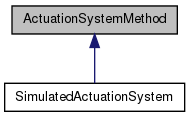
\includegraphics[width=214pt]{class_actuation_system_method__inherit__graph}
\end{center}
\end{figure}
\subsection*{\-Public \-Types}
\begin{DoxyCompactItemize}
\item 
\hypertarget{class_actuation_system_method_ab79e392d3f9966254b2e210b50c185c5}{typedef \*
\hyperlink{class_s_e2_belief_space}{\-Motion\-Model\-Method\-::\-Space\-Type} {\bfseries \-Space\-Type}}\label{class_actuation_system_method_ab79e392d3f9966254b2e210b50c185c5}

\item 
\hypertarget{class_actuation_system_method_a9d369d1bb1183b3d312ad6ea637d247d}{typedef \*
\hyperlink{class_s_e2_belief_space_1_1_state_type}{\-Motion\-Model\-Method\-::\-State\-Type} {\bfseries \-State\-Type}}\label{class_actuation_system_method_a9d369d1bb1183b3d312ad6ea637d247d}

\item 
\hypertarget{class_actuation_system_method_afa097c36486db5da11865e8b4d19a019}{typedef \*
\-Motion\-Model\-Method\-::\-Control\-Type {\bfseries \-Control\-Type}}\label{class_actuation_system_method_afa097c36486db5da11865e8b4d19a019}

\item 
\hypertarget{class_actuation_system_method_abe58ca32071c91cf6ed98250c23c6891}{typedef \*
\-Observation\-Model\-Method\-::\-Observation\-Type {\bfseries \-Observation\-Type}}\label{class_actuation_system_method_abe58ca32071c91cf6ed98250c23c6891}

\item 
\hypertarget{class_actuation_system_method_a8c0f4c72ee875c8a1de4e2f5da3f1921}{typedef boost\-::shared\-\_\-ptr\*
$<$ \hyperlink{class_actuation_system_method}{\-Actuation\-System\-Method} $>$ {\bfseries \-Actuation\-System\-Pointer}}\label{class_actuation_system_method_a8c0f4c72ee875c8a1de4e2f5da3f1921}

\item 
\hypertarget{class_actuation_system_method_adcac81ce42938d3c0532b5d995168503}{typedef \*
\-Observation\-Model\-Method\-::\-Observation\-Model\-Pointer {\bfseries \-Observation\-Model\-Pointer}}\label{class_actuation_system_method_adcac81ce42938d3c0532b5d995168503}

\item 
\hypertarget{class_actuation_system_method_a9c74f0393051387d16387c63ca78834a}{typedef \*
\-Motion\-Model\-Method\-::\-Motion\-Model\-Pointer {\bfseries \-Motion\-Model\-Pointer}}\label{class_actuation_system_method_a9c74f0393051387d16387c63ca78834a}

\end{DoxyCompactItemize}
\subsection*{\-Public \-Member \-Functions}
\begin{DoxyCompactItemize}
\item 
\hypertarget{class_actuation_system_method_a140d1929d9ba39eeda45233ede7291f5}{{\bfseries \-Actuation\-System\-Method} (\-Motion\-Model\-Pointer mm, \-Observation\-Model\-Pointer om)}\label{class_actuation_system_method_a140d1929d9ba39eeda45233ede7291f5}

\item 
\hypertarget{class_actuation_system_method_a8380694aec22c19388bc463af9d0c12d}{virtual void {\bfseries apply\-Control} (\-Control\-Type \&u)=0}\label{class_actuation_system_method_a8380694aec22c19388bc463af9d0c12d}

\item 
\hypertarget{class_actuation_system_method_a68d37d0f01992b30a014adbd971d7d6f}{virtual \-Observation\-Type {\bfseries get\-Observation} ()=0}\label{class_actuation_system_method_a68d37d0f01992b30a014adbd971d7d6f}

\item 
\hypertarget{class_actuation_system_method_aac1d548e63d19bde0dcf6b44bf3b644f}{virtual bool {\bfseries check\-Collision} ()=0}\label{class_actuation_system_method_aac1d548e63d19bde0dcf6b44bf3b644f}

\item 
\hypertarget{class_actuation_system_method_a96352d97bd055a0cc33871f9afde9456}{virtual void {\bfseries set\-Belief} (const ompl\-::base\-::\-State $\ast$state)=0}\label{class_actuation_system_method_a96352d97bd055a0cc33871f9afde9456}

\item 
\hypertarget{class_actuation_system_method_a85738bc14a387b5c04c266b046768c34}{virtual void {\bfseries set\-True\-State} (const ompl\-::base\-::\-State $\ast$state)=0}\label{class_actuation_system_method_a85738bc14a387b5c04c266b046768c34}

\item 
\hypertarget{class_actuation_system_method_a20ef48b160e9072fd28aadc992fd66d5}{virtual ompl\-::base\-::\-State $\ast$ {\bfseries get\-True\-State} ()=0}\label{class_actuation_system_method_a20ef48b160e9072fd28aadc992fd66d5}

\item 
\hypertarget{class_actuation_system_method_a75449aaf949ef6fbe19b3ef0d2a60d27}{virtual \-Motion\-Model\-Pointer {\bfseries get\-Motion\-Model} ()=0}\label{class_actuation_system_method_a75449aaf949ef6fbe19b3ef0d2a60d27}

\item 
\hypertarget{class_actuation_system_method_a229e5c520570c541218640e5ff25ae5c}{virtual \-Observation\-Model\-Pointer {\bfseries get\-Observation\-Model} ()=0}\label{class_actuation_system_method_a229e5c520570c541218640e5ff25ae5c}

\end{DoxyCompactItemize}
\subsection*{\-Protected \-Attributes}
\begin{DoxyCompactItemize}
\item 
\hypertarget{class_actuation_system_method_a64ced37059fb1bb538f9b2a26ea018f4}{\-Motion\-Model\-Pointer {\bfseries motion\-Model\-\_\-}}\label{class_actuation_system_method_a64ced37059fb1bb538f9b2a26ea018f4}

\item 
\hypertarget{class_actuation_system_method_a30d8ec99ae45fd0c3233b85e9ef4093d}{\-Observation\-Model\-Pointer {\bfseries observation\-Model\-\_\-}}\label{class_actuation_system_method_a30d8ec99ae45fd0c3233b85e9ef4093d}

\end{DoxyCompactItemize}


\-The documentation for this class was generated from the following file\-:\begin{DoxyCompactItemize}
\item 
include/\-Actuation\-Systems/\-Actuation\-System\-Method.\-h\end{DoxyCompactItemize}

\hypertarget{class_cam_aruco2_d_observation_model}{\section{\-Cam\-Aruco2\-D\-Observation\-Model \-Class \-Reference}
\label{class_cam_aruco2_d_observation_model}\index{\-Cam\-Aruco2\-D\-Observation\-Model@{\-Cam\-Aruco2\-D\-Observation\-Model}}
}


\-Inheritance diagram for \-Cam\-Aruco2\-D\-Observation\-Model\-:\nopagebreak
\begin{figure}[H]
\begin{center}
\leavevmode
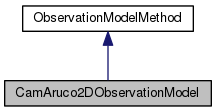
\includegraphics[width=234pt]{class_cam_aruco2_d_observation_model__inherit__graph}
\end{center}
\end{figure}


\-Collaboration diagram for \-Cam\-Aruco2\-D\-Observation\-Model\-:\nopagebreak
\begin{figure}[H]
\begin{center}
\leavevmode
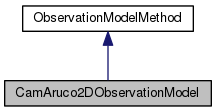
\includegraphics[width=234pt]{class_cam_aruco2_d_observation_model__coll__graph}
\end{center}
\end{figure}
\subsection*{\-Public \-Types}
\begin{DoxyCompactItemize}
\item 
\hypertarget{class_cam_aruco2_d_observation_model_a227cf56e4ad62f5fec7c88b5b8c5a403}{typedef \*
\-Observation\-Model\-Method\-::\-Observation\-Type {\bfseries \-Observation\-Type}}\label{class_cam_aruco2_d_observation_model_a227cf56e4ad62f5fec7c88b5b8c5a403}

\item 
\hypertarget{class_cam_aruco2_d_observation_model_a45378bb9e9708b75b6d7cea400c4e179}{typedef \*
\-Observation\-Model\-Method\-::\-Noise\-Type {\bfseries \-Obs\-Noise\-Type}}\label{class_cam_aruco2_d_observation_model_a45378bb9e9708b75b6d7cea400c4e179}

\item 
\hypertarget{class_cam_aruco2_d_observation_model_aabb4595d4a78f07033daee230dd3b7e8}{typedef arma\-::mat {\bfseries \-Jacobian\-Type}}\label{class_cam_aruco2_d_observation_model_aabb4595d4a78f07033daee230dd3b7e8}

\end{DoxyCompactItemize}
\subsection*{\-Public \-Member \-Functions}
\begin{DoxyCompactItemize}
\item 
\hypertarget{class_cam_aruco2_d_observation_model_aedf847cd06f4f836797f5dbe9f99fca2}{{\bfseries \-Cam\-Aruco2\-D\-Observation\-Model} (const char $\ast$path\-To\-Setup\-File)}\label{class_cam_aruco2_d_observation_model_aedf847cd06f4f836797f5dbe9f99fca2}

\item 
\-Observation\-Type \hyperlink{class_cam_aruco2_d_observation_model_a244fd43dca1734b68bf1379b2be285d2}{get\-Observation} (const ompl\-::base\-::\-State $\ast$state, bool is\-Simulation)
\item 
\hypertarget{class_cam_aruco2_d_observation_model_a0c1869cfc821819f3fd014a9acb45a77}{\-Observation\-Type {\bfseries get\-Observation\-Prediction} (const ompl\-::base\-::\-State $\ast$state, const \-Observation\-Type \&\-Zg)}\label{class_cam_aruco2_d_observation_model_a0c1869cfc821819f3fd014a9acb45a77}

\item 
\hypertarget{class_cam_aruco2_d_observation_model_a820641c18621356b468d6646e9c35111}{\-Jacobian\-Type {\bfseries get\-Observation\-Jacobian} (const ompl\-::base\-::\-State $\ast$state, const \-Obs\-Noise\-Type \&v, const \-Observation\-Type \&z)}\label{class_cam_aruco2_d_observation_model_a820641c18621356b468d6646e9c35111}

\item 
\hypertarget{class_cam_aruco2_d_observation_model_ac1452891ef75d5dde2cf05ee628aa2fb}{\-Jacobian\-Type {\bfseries get\-Noise\-Jacobian} (const ompl\-::base\-::\-State $\ast$state, const \-Obs\-Noise\-Type \&v, const \-Observation\-Type \&z)}\label{class_cam_aruco2_d_observation_model_ac1452891ef75d5dde2cf05ee628aa2fb}

\item 
\hypertarget{class_cam_aruco2_d_observation_model_a61876ff06e81a6fd556f06ef562e3b3c}{\-Observation\-Type {\bfseries compute\-Innovation} (const ompl\-::base\-::\-State $\ast$predicted\-State, const \-Observation\-Type \&\-Zg)}\label{class_cam_aruco2_d_observation_model_a61876ff06e81a6fd556f06ef562e3b3c}

\item 
\hypertarget{class_cam_aruco2_d_observation_model_a32074e56674e8089dbcce9cf603af398}{arma\-::mat {\bfseries get\-Observation\-Noise\-Covariance} (const ompl\-::base\-::\-State $\ast$state, const \-Observation\-Type \&z)}\label{class_cam_aruco2_d_observation_model_a32074e56674e8089dbcce9cf603af398}

\item 
\hypertarget{class_cam_aruco2_d_observation_model_aefa9e3d5d9d40de6ef197d3e25b190bd}{bool {\bfseries is\-Landmark\-Visible} (const arma\-::colvec x\-Vec, const arma\-::colvec \&landmark, double \&range, double \&bearing, double \&viewing\-Angle)}\label{class_cam_aruco2_d_observation_model_aefa9e3d5d9d40de6ef197d3e25b190bd}

\item 
\hypertarget{class_cam_aruco2_d_observation_model_addfed85e3589e4525bb8f2fa03657a01}{bool {\bfseries is\-State\-Observable} (const ompl\-::base\-::\-State $\ast$state)}\label{class_cam_aruco2_d_observation_model_addfed85e3589e4525bb8f2fa03657a01}

\end{DoxyCompactItemize}
\subsection*{\-Private \-Member \-Functions}
\begin{DoxyCompactItemize}
\item 
\hypertarget{class_cam_aruco2_d_observation_model_a616ee9ed0c516b0c9fc0eeb6d492ac3f}{\-Observation\-Type {\bfseries remove\-Spurious\-Observations} (const \-Observation\-Type \&\-Zg)}\label{class_cam_aruco2_d_observation_model_a616ee9ed0c516b0c9fc0eeb6d492ac3f}

\item 
\hypertarget{class_cam_aruco2_d_observation_model_a105506bb8493e23b2a70f4c811577ea3}{void {\bfseries load\-Landmarks} (const char $\ast$path\-To\-Setup\-File)}\label{class_cam_aruco2_d_observation_model_a105506bb8493e23b2a70f4c811577ea3}

\item 
\hypertarget{class_cam_aruco2_d_observation_model_af2586c7b2c3ab276f1c13ba1e3ba71f3}{void {\bfseries load\-Parameters} (const char $\ast$path\-To\-Setup\-File)}\label{class_cam_aruco2_d_observation_model_af2586c7b2c3ab276f1c13ba1e3ba71f3}

\end{DoxyCompactItemize}
\subsection*{\-Private \-Attributes}
\begin{DoxyCompactItemize}
\item 
\hypertarget{class_cam_aruco2_d_observation_model_a06626a8304e171f284bd550d02b6f63c}{std\-::vector$<$ arma\-::colvec $>$ {\bfseries landmarks\-\_\-}}\label{class_cam_aruco2_d_observation_model_a06626a8304e171f284bd550d02b6f63c}

\end{DoxyCompactItemize}
\subsection*{\-Static \-Private \-Attributes}
\begin{DoxyCompactItemize}
\item 
\hypertarget{class_cam_aruco2_d_observation_model_a88056dea15d6aeaafa5a11e2226eab21}{static const int {\bfseries state\-Dim} = 3}\label{class_cam_aruco2_d_observation_model_a88056dea15d6aeaafa5a11e2226eab21}

\item 
\hypertarget{class_cam_aruco2_d_observation_model_a8cfcef2cce47d94816e6d2692102df6f}{static const int {\bfseries single\-Observation\-Dim} = 4}\label{class_cam_aruco2_d_observation_model_a8cfcef2cce47d94816e6d2692102df6f}

\item 
\hypertarget{class_cam_aruco2_d_observation_model_a0b4eff8ec91d2cae6a2d37495e9541d3}{static const int {\bfseries landmark\-Info\-Dim} = 2}\label{class_cam_aruco2_d_observation_model_a0b4eff8ec91d2cae6a2d37495e9541d3}

\item 
\hypertarget{class_cam_aruco2_d_observation_model_a1750ab1c5ac476d09da804e7a92576f5}{static const int {\bfseries num\-Landmarks\-For\-Observability} = 2}\label{class_cam_aruco2_d_observation_model_a1750ab1c5ac476d09da804e7a92576f5}

\end{DoxyCompactItemize}


\subsection{\-Member \-Function \-Documentation}
\hypertarget{class_cam_aruco2_d_observation_model_a244fd43dca1734b68bf1379b2be285d2}{\index{\-Cam\-Aruco2\-D\-Observation\-Model@{\-Cam\-Aruco2\-D\-Observation\-Model}!get\-Observation@{get\-Observation}}
\index{get\-Observation@{get\-Observation}!CamAruco2DObservationModel@{\-Cam\-Aruco2\-D\-Observation\-Model}}
\subsubsection[{get\-Observation}]{\setlength{\rightskip}{0pt plus 5cm}\-Cam\-Aruco2\-D\-Observation\-Model\-::\-Observation\-Type {\bf \-Cam\-Aruco2\-D\-Observation\-Model\-::get\-Observation} (
\begin{DoxyParamCaption}
\item[{const ompl\-::base\-::\-State $\ast$}]{state, }
\item[{bool}]{is\-Simulation}
\end{DoxyParamCaption}
)\hspace{0.3cm}{\ttfamily  \mbox{[}virtual\mbox{]}}}}\label{class_cam_aruco2_d_observation_model_a244fd43dca1734b68bf1379b2be285d2}
z = h(x,v) get the observation for a given configuration. 1. is\-Simulation= true , corrupted by noise from a given distribution 2. is\-Simulation=false , noise free obs 

\-Implements \hyperlink{class_observation_model_method_af1a30aad975576ae8f16042a8ee8276b}{\-Observation\-Model\-Method}.



\-The documentation for this class was generated from the following files\-:\begin{DoxyCompactItemize}
\item 
include/\-Observation\-Models/\-Cam\-Aruco2\-D\-Observation\-Model.\-h\item 
src/\-Observation\-Models/\-Cam\-Aruco2\-D\-Observation\-Model.\-cpp\end{DoxyCompactItemize}

\hypertarget{class_controller}{\section{\-Controller$<$ \-Separated\-Controller\-Type, \-Filter\-Type $>$ \-Class \-Template \-Reference}
\label{class_controller}\index{\-Controller$<$ Separated\-Controller\-Type, Filter\-Type $>$@{\-Controller$<$ Separated\-Controller\-Type, Filter\-Type $>$}}
}


\-Base class for \hyperlink{class_controller}{\-Controller}. \-A controller's task is to use the filter to estimate the belief robot's state and generate control commands using the separated controller. \-For example by fusing an \-L\-Q\-R and \-Kalman \-Filter we generate an \-L\-Q\-G controller.  




{\ttfamily \#include $<$\-Controller.\-h$>$}



\-Collaboration diagram for \-Controller$<$ \-Separated\-Controller\-Type, \-Filter\-Type $>$\-:\nopagebreak
\begin{figure}[H]
\begin{center}
\leavevmode
\includegraphics[width=317pt]{class_controller__coll__graph}
\end{center}
\end{figure}
\subsection*{\-Public \-Types}
\begin{DoxyCompactItemize}
\item 
\hypertarget{class_controller_aa08894881f64205d60cf7569370af8e1}{typedef \*
\hyperlink{class_s_e2_belief_space}{\-Motion\-Model\-Method\-::\-Space\-Type} {\bfseries \-Space\-Type}}\label{class_controller_aa08894881f64205d60cf7569370af8e1}

\item 
\hypertarget{class_controller_a8fc267f97b0a2a3e1c2b97d791805b5c}{typedef \*
\hyperlink{class_s_e2_belief_space_1_1_state_type}{\-Motion\-Model\-Method\-::\-State\-Type} {\bfseries \-State\-Type}}\label{class_controller_a8fc267f97b0a2a3e1c2b97d791805b5c}

\item 
\hypertarget{class_controller_a0ae807c4f455600c8ca827b816bbd40d}{typedef \*
firm\-::\-Space\-Information\-::\-Space\-Information\-Ptr {\bfseries \-Space\-Information\-Ptr}}\label{class_controller_a0ae807c4f455600c8ca827b816bbd40d}

\item 
\hypertarget{class_controller_ab388284a58474044cc503e876cf0bc7f}{typedef \*
\-Motion\-Model\-Method\-::\-Control\-Type {\bfseries \-Control\-Type}}\label{class_controller_ab388284a58474044cc503e876cf0bc7f}

\item 
\hypertarget{class_controller_a734aecb1a1538fb2154f238796b26d0d}{typedef \*
\-Observation\-Model\-Method\-::\-Observation\-Type {\bfseries \-Observation\-Type}}\label{class_controller_a734aecb1a1538fb2154f238796b26d0d}

\item 
\hypertarget{class_controller_a5b6a5e6d71e96c200e57a52542a4a493}{typedef \*
\-Motion\-Model\-Method\-::\-Motion\-Model\-Pointer {\bfseries \-Motion\-Model\-Pointer}}\label{class_controller_a5b6a5e6d71e96c200e57a52542a4a493}

\item 
\hypertarget{class_controller_a3c4329f9c227302f331c3c2b78cda5d7}{typedef \*
\-Observation\-Model\-Method\-::\-Observation\-Model\-Pointer {\bfseries \-Observation\-Model\-Pointer}}\label{class_controller_a3c4329f9c227302f331c3c2b78cda5d7}

\end{DoxyCompactItemize}
\subsection*{\-Public \-Member \-Functions}
\begin{DoxyCompactItemize}
\item 
\hypertarget{class_controller_ab3f614e32fa25535809e056ce2492ab3}{\hyperlink{class_controller_ab3f614e32fa25535809e056ce2492ab3}{\-Controller} ()}\label{class_controller_ab3f614e32fa25535809e056ce2492ab3}

\begin{DoxyCompactList}\small\item\em \-Constructor. \end{DoxyCompactList}\item 
\hypertarget{class_controller_a50a65edd2cf9fcce0cca465cbc3d527d}{\hyperlink{class_controller_a50a65edd2cf9fcce0cca465cbc3d527d}{\-Controller} (const ompl\-::base\-::\-State $\ast$goal, const std\-::vector$<$ ompl\-::base\-::\-State $\ast$ $>$ \&nominal\-Xs, const std\-::vector$<$ ompl\-::control\-::\-Control $\ast$ $>$ \&nominal\-Us, const firm\-::\-Space\-Information\-::\-Space\-Information\-Ptr si)}\label{class_controller_a50a65edd2cf9fcce0cca465cbc3d527d}

\begin{DoxyCompactList}\small\item\em \-Constructor. \end{DoxyCompactList}\item 
\hypertarget{class_controller_a01cbbc1435d0a4ed8733332bef6d7342}{virtual bool \hyperlink{class_controller_a01cbbc1435d0a4ed8733332bef6d7342}{\-Execute} (const ompl\-::base\-::\-State $\ast$start\-State, ompl\-::base\-::\-State $\ast$end\-State, ompl\-::base\-::\-Cost \&execution\-Cost, bool construction\-Mode=true)}\label{class_controller_a01cbbc1435d0a4ed8733332bef6d7342}

\begin{DoxyCompactList}\small\item\em \-Execute the controller i.\-e. take the system from start to end state of edge. \end{DoxyCompactList}\item 
\hypertarget{class_controller_aba227cad46f73fab5fcf37b41cae71a9}{virtual ompl\-::base\-::\-State $\ast$ \hyperlink{class_controller_aba227cad46f73fab5fcf37b41cae71a9}{\-Stabilize} (const ompl\-::base\-::\-State $\ast$start\-State)}\label{class_controller_aba227cad46f73fab5fcf37b41cae71a9}

\begin{DoxyCompactList}\small\item\em \-Stabilize the system to an existing \hyperlink{class_f_i_r_m}{\-F\-I\-R\-M} node. \end{DoxyCompactList}\item 
\hypertarget{class_controller_ab80efffa3b03aa4d1d10c0bf82675201}{virtual bool \hyperlink{class_controller_ab80efffa3b03aa4d1d10c0bf82675201}{is\-Terminated} (const ompl\-::base\-::\-State $\ast$state, const size\-\_\-t t)}\label{class_controller_ab80efffa3b03aa4d1d10c0bf82675201}

\begin{DoxyCompactList}\small\item\em \-Check whether the controller has satisfied its termination condition for e.\-g. reached target state. \end{DoxyCompactList}\item 
\hypertarget{class_controller_a64c3c47732f138326490303858133ae7}{virtual void \hyperlink{class_controller_a64c3c47732f138326490303858133ae7}{\-Evolve} (const ompl\-::base\-::\-State $\ast$state, size\-\_\-t t, ompl\-::base\-::\-State $\ast$next\-State)}\label{class_controller_a64c3c47732f138326490303858133ae7}

\begin{DoxyCompactList}\small\item\em \-Evolve the controller over a single time step, i.\-e. apply control, predict, get observation, update. \end{DoxyCompactList}\item 
\hypertarget{class_controller_a848b1e5a3dc6d36c3ede121b7461d896}{ompl\-::base\-::\-State $\ast$ \hyperlink{class_controller_a848b1e5a3dc6d36c3ede121b7461d896}{get\-Goal} ()}\label{class_controller_a848b1e5a3dc6d36c3ede121b7461d896}

\begin{DoxyCompactList}\small\item\em get the controllers goal state \end{DoxyCompactList}\item 
\hypertarget{class_controller_ac0b9c339df7157c73d61b7064f88483c}{void \hyperlink{class_controller_ac0b9c339df7157c73d61b7064f88483c}{set\-Space\-Information} (\-Space\-Information\-Ptr si)}\label{class_controller_ac0b9c339df7157c73d61b7064f88483c}

\begin{DoxyCompactList}\small\item\em \-Set the space information of the planning problem. \end{DoxyCompactList}\item 
\hypertarget{class_controller_a2aa89a4cd76ba7fb6ad717d608b8c355}{size\-\_\-t \hyperlink{class_controller_a2aa89a4cd76ba7fb6ad717d608b8c355}{\-Length} ()}\label{class_controller_a2aa89a4cd76ba7fb6ad717d608b8c355}

\begin{DoxyCompactList}\small\item\em \-Return the number of linear systems. \end{DoxyCompactList}\end{DoxyCompactItemize}
\subsection*{\-Static \-Public \-Member \-Functions}
\begin{DoxyCompactItemize}
\item 
\hypertarget{class_controller_a665b0a9cab38c11e575681944e2c8d8a}{static void \hyperlink{class_controller_a665b0a9cab38c11e575681944e2c8d8a}{set\-Node\-Reached\-Angle} (double angle)}\label{class_controller_a665b0a9cab38c11e575681944e2c8d8a}

\begin{DoxyCompactList}\small\item\em \-Set the node\-Reached angle. \end{DoxyCompactList}\item 
\hypertarget{class_controller_a5d394a75a6d1cf325fda099b23c91a2f}{static void \hyperlink{class_controller_a5d394a75a6d1cf325fda099b23c91a2f}{set\-Node\-Reached\-Distance} (double d)}\label{class_controller_a5d394a75a6d1cf325fda099b23c91a2f}

\begin{DoxyCompactList}\small\item\em \-Set the distance at which we assume the robot has reached a target node. \end{DoxyCompactList}\item 
\hypertarget{class_controller_a2e27a2fbd5d1c83d918e05da91302863}{static void \hyperlink{class_controller_a2e27a2fbd5d1c83d918e05da91302863}{set\-Max\-Tries} (double maxtries)}\label{class_controller_a2e27a2fbd5d1c83d918e05da91302863}

\begin{DoxyCompactList}\small\item\em \-The max number of attempts to align with node. \end{DoxyCompactList}\item 
\hypertarget{class_controller_aacd25b8b49bcec685b0ec284bb9694d6}{static void \hyperlink{class_controller_aacd25b8b49bcec685b0ec284bb9694d6}{set\-Max\-Trajectory\-Deviation} (double dev)}\label{class_controller_aacd25b8b49bcec685b0ec284bb9694d6}

\begin{DoxyCompactList}\small\item\em \-Set the maximum trajectory deviation before which to replan. \end{DoxyCompactList}\end{DoxyCompactItemize}
\subsection*{\-Private \-Attributes}
\begin{DoxyCompactItemize}
\item 
\hypertarget{class_controller_a34912a3b87662649231e2d096882c454}{\-Space\-Information\-Ptr \hyperlink{class_controller_a34912a3b87662649231e2d096882c454}{si\-\_\-}}\label{class_controller_a34912a3b87662649231e2d096882c454}

\begin{DoxyCompactList}\small\item\em \-The pointer to the space information. \end{DoxyCompactList}\item 
\hypertarget{class_controller_acb68b603afc759b4e62b8c6db8125671}{std\-::vector$<$ \hyperlink{class_linear_system}{\-Linear\-System} $>$ \hyperlink{class_controller_acb68b603afc759b4e62b8c6db8125671}{lss\-\_\-}}\label{class_controller_acb68b603afc759b4e62b8c6db8125671}

\begin{DoxyCompactList}\small\item\em \-The vector of linear systems. \-The linear systems basically represent the system state at a point in the open loop trajectory. \end{DoxyCompactList}\item 
\hypertarget{class_controller_a040da727bdc40ab69f0c3e4033bc9df9}{\-Separated\-Controller\-Type \hyperlink{class_controller_a040da727bdc40ab69f0c3e4033bc9df9}{separated\-Controller\-\_\-}}\label{class_controller_a040da727bdc40ab69f0c3e4033bc9df9}

\begin{DoxyCompactList}\small\item\em \-The separated controller used to generate the commands that are sent to the robot. \end{DoxyCompactList}\item 
\hypertarget{class_controller_a9ff37d34a8a9a20f606c501d2ab5cb2e}{\-Filter\-Type \hyperlink{class_controller_a9ff37d34a8a9a20f606c501d2ab5cb2e}{filter\-\_\-}}\label{class_controller_a9ff37d34a8a9a20f606c501d2ab5cb2e}

\begin{DoxyCompactList}\small\item\em \-The filter used to estimate the robot belief. \end{DoxyCompactList}\item 
\hypertarget{class_controller_a4e5e3c0828c9e0d216e7d53f3625d9b4}{ompl\-::base\-::\-State $\ast$ \hyperlink{class_controller_a4e5e3c0828c9e0d216e7d53f3625d9b4}{goal\-\_\-}}\label{class_controller_a4e5e3c0828c9e0d216e7d53f3625d9b4}

\begin{DoxyCompactList}\small\item\em \-The target node to which the controller drives the robot. \end{DoxyCompactList}\item 
\hypertarget{class_controller_adb2235b65db786dbd287e0b57a42b959}{int \hyperlink{class_controller_adb2235b65db786dbd287e0b57a42b959}{tries\-\_\-}}\label{class_controller_adb2235b65db786dbd287e0b57a42b959}

\begin{DoxyCompactList}\small\item\em \-Tracks the current number of time steps the robot has executed to align with goal node. \end{DoxyCompactList}\item 
\hypertarget{class_controller_aeddadf542e253ff266e596eb0574c3de}{double \hyperlink{class_controller_aeddadf542e253ff266e596eb0574c3de}{max\-Exec\-Time\-\_\-}}\label{class_controller_aeddadf542e253ff266e596eb0574c3de}

\begin{DoxyCompactList}\small\item\em \-The maximum time for which a controller can be executed. \-We need this bound as we cannot let a controller execute indefinitely. \-This avoids situations when the robot has deviated or collided and the current controller is no longer capable of driving the robot to the goal. \end{DoxyCompactList}\item 
\hypertarget{class_controller_a1288c6ee79e962bba7421ffb59bae047}{bool \hyperlink{class_controller_a1288c6ee79e962bba7421ffb59bae047}{debug\-\_\-}}\label{class_controller_a1288c6ee79e962bba7421ffb59bae047}

\begin{DoxyCompactList}\small\item\em \-The debug mode, if true, controller is verbose. \end{DoxyCompactList}\end{DoxyCompactItemize}
\subsection*{\-Static \-Private \-Attributes}
\begin{DoxyCompactItemize}
\item 
\hypertarget{class_controller_a93ec5b0a3ae4e7229cb63f659e1b6e1d}{static double \hyperlink{class_controller_a93ec5b0a3ae4e7229cb63f659e1b6e1d}{node\-Reached\-Angle\-\_\-} = -\/1}\label{class_controller_a93ec5b0a3ae4e7229cb63f659e1b6e1d}

\begin{DoxyCompactList}\small\item\em \-If the robot's heading is deviated from the target heading by less than the node\-Reached\-Angle\-\_\- then the robot is assumed to have alligned with the target heading. \-Used for node reachability checking. \end{DoxyCompactList}\item 
\hypertarget{class_controller_a2688f277c2087c527c67eec19b2a3c70}{static double \hyperlink{class_controller_a2688f277c2087c527c67eec19b2a3c70}{node\-Reached\-Distance\-\_\-} = -\/1}\label{class_controller_a2688f277c2087c527c67eec19b2a3c70}

\begin{DoxyCompactList}\small\item\em \-The distance at which we assume the robot has reached a target node. \-Reaching the exact node location is almost impractical for real systems. \-We assume the robot has reached if it is within a certain radius of the target. \end{DoxyCompactList}\item 
\hypertarget{class_controller_a430b93daf349b2172311924d69b44c08}{static double \hyperlink{class_controller_a430b93daf349b2172311924d69b44c08}{max\-Tries\-\_\-} = -\/1}\label{class_controller_a430b93daf349b2172311924d69b44c08}

\begin{DoxyCompactList}\small\item\em \-The max number of tries to align with target node. \end{DoxyCompactList}\item 
\hypertarget{class_controller_a1999422f369674236a5ae9b83ef6a6b1}{static double \hyperlink{class_controller_a1999422f369674236a5ae9b83ef6a6b1}{nominal\-Traj\-Deviation\-Threshold\-\_\-} = -\/1}\label{class_controller_a1999422f369674236a5ae9b83ef6a6b1}

\begin{DoxyCompactList}\small\item\em \-The maximum deviation from the nominal trajectory beyond which the robot must replan. \end{DoxyCompactList}\end{DoxyCompactItemize}


\subsection{\-Detailed \-Description}
\subsubsection*{template$<$class \-Separated\-Controller\-Type, class \-Filter\-Type$>$class Controller$<$ Separated\-Controller\-Type, Filter\-Type $>$}

\-Base class for \hyperlink{class_controller}{\-Controller}. \-A controller's task is to use the filter to estimate the belief robot's state and generate control commands using the separated controller. \-For example by fusing an \-L\-Q\-R and \-Kalman \-Filter we generate an \-L\-Q\-G controller. 

\-The documentation for this class was generated from the following files\-:\begin{DoxyCompactItemize}
\item 
include/\-Controllers/\-Controller.\-h\item 
src/\-Controllers/\-Controller.\-cpp\end{DoxyCompactItemize}

\hypertarget{struct_double_value_comp}{\section{\-Double\-Value\-Comp \-Struct \-Reference}
\label{struct_double_value_comp}\index{\-Double\-Value\-Comp@{\-Double\-Value\-Comp}}
}
\subsection*{\-Public \-Member \-Functions}
\begin{DoxyCompactItemize}
\item 
\hypertarget{struct_double_value_comp_ac6d9c50d9d2897ff6c452c71114d585e}{{\footnotesize template$<$typename K\-V\-P1 , typename K\-V\-P2 $>$ }\\bool {\bfseries operator()} (const \-K\-V\-P1 \&kvp1, const \-K\-V\-P2 \&kvp2) const }\label{struct_double_value_comp_ac6d9c50d9d2897ff6c452c71114d585e}

\item 
\hypertarget{struct_double_value_comp_ac6d9c50d9d2897ff6c452c71114d585e}{{\footnotesize template$<$typename K\-V\-P1 , typename K\-V\-P2 $>$ }\\bool {\bfseries operator()} (const \-K\-V\-P1 \&kvp1, const \-K\-V\-P2 \&kvp2) const }\label{struct_double_value_comp_ac6d9c50d9d2897ff6c452c71114d585e}

\item 
\hypertarget{struct_double_value_comp_ac6d9c50d9d2897ff6c452c71114d585e}{{\footnotesize template$<$typename K\-V\-P1 , typename K\-V\-P2 $>$ }\\bool {\bfseries operator()} (const \-K\-V\-P1 \&kvp1, const \-K\-V\-P2 \&kvp2) const }\label{struct_double_value_comp_ac6d9c50d9d2897ff6c452c71114d585e}

\end{DoxyCompactItemize}


\-The documentation for this struct was generated from the following files\-:\begin{DoxyCompactItemize}
\item 
src/\-Planner/\-F\-I\-R\-M-\/old-\/v2.\-cpp\item 
src/\-Planner/\-F\-I\-R\-M-\/old.\-cpp\item 
src/\-Planner/\-F\-I\-R\-M.\-cpp\end{DoxyCompactItemize}

\hypertarget{struct_f_i_r_m_1_1edge__flags__t}{\section{\-F\-I\-R\-M\-:\-:edge\-\_\-flags\-\_\-t \-Struct \-Reference}
\label{struct_f_i_r_m_1_1edge__flags__t}\index{\-F\-I\-R\-M\-::edge\-\_\-flags\-\_\-t@{\-F\-I\-R\-M\-::edge\-\_\-flags\-\_\-t}}
}
\subsection*{\-Public \-Types}
\begin{DoxyCompactItemize}
\item 
\hypertarget{struct_f_i_r_m_1_1edge__flags__t_a37a098e50779a7a6772be2ffa85502d4}{typedef boost\-::edge\-\_\-property\-\_\-tag {\bfseries kind}}\label{struct_f_i_r_m_1_1edge__flags__t_a37a098e50779a7a6772be2ffa85502d4}

\end{DoxyCompactItemize}


\-The documentation for this struct was generated from the following file\-:\begin{DoxyCompactItemize}
\item 
include/\-Planner/\-F\-I\-R\-M.\-h\end{DoxyCompactItemize}

\hypertarget{struct_edge_comp}{\section{\-Edge\-Comp \-Struct \-Reference}
\label{struct_edge_comp}\index{\-Edge\-Comp@{\-Edge\-Comp}}
}
\subsection*{\-Public \-Member \-Functions}
\begin{DoxyCompactItemize}
\item 
\hypertarget{struct_edge_comp_a90f9e5edf3656c4b574d58a2323805dc}{{\footnotesize template$<$typename E\-I\-D1 , typename E\-I\-D2 $>$ }\\bool {\bfseries operator()} (const \-E\-I\-D1 \&e1, const \-E\-I\-D2 \&e2) const }\label{struct_edge_comp_a90f9e5edf3656c4b574d58a2323805dc}

\end{DoxyCompactItemize}


\-The documentation for this struct was generated from the following file\-:\begin{DoxyCompactItemize}
\item 
src/\-Planner/\-F\-I\-R\-M.\-cpp\end{DoxyCompactItemize}

\input{struct_ti_xml_base_1_1_entity}
\hypertarget{class_extended_k_f}{\section{\-Extended\-K\-F \-Class \-Reference}
\label{class_extended_k_f}\index{\-Extended\-K\-F@{\-Extended\-K\-F}}
}


\-Implementation of the \-Extended \-Kalman \-Filter.  




{\ttfamily \#include $<$\-Extended\-K\-F.\-h$>$}



\-Inheritance diagram for \-Extended\-K\-F\-:\nopagebreak
\begin{figure}[H]
\begin{center}
\leavevmode
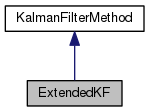
\includegraphics[width=184pt]{class_extended_k_f__inherit__graph}
\end{center}
\end{figure}


\-Collaboration diagram for \-Extended\-K\-F\-:\nopagebreak
\begin{figure}[H]
\begin{center}
\leavevmode
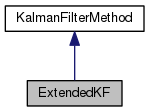
\includegraphics[width=184pt]{class_extended_k_f__coll__graph}
\end{center}
\end{figure}
\subsection*{\-Public \-Types}
\begin{DoxyCompactItemize}
\item 
\hypertarget{class_extended_k_f_a14edd0da9fb8029c87fb0206490e10b3}{typedef \*
\-Motion\-Model\-Method\-::\-Control\-Type {\bfseries \-Control\-Type}}\label{class_extended_k_f_a14edd0da9fb8029c87fb0206490e10b3}

\item 
\hypertarget{class_extended_k_f_a577b350233488edad44145be188b8838}{typedef \*
\hyperlink{class_s_e2_belief_space}{\-Motion\-Model\-Method\-::\-Space\-Type} {\bfseries \-Space\-Type}}\label{class_extended_k_f_a577b350233488edad44145be188b8838}

\item 
\hypertarget{class_extended_k_f_a390468694f87826805dc6b97e37da8ea}{typedef \*
\hyperlink{class_s_e2_belief_space_1_1_state_type}{\-Motion\-Model\-Method\-::\-State\-Type} {\bfseries \-State\-Type}}\label{class_extended_k_f_a390468694f87826805dc6b97e37da8ea}

\item 
\hypertarget{class_extended_k_f_a77ebe1a32d7ec95c8cda310ad4623e8e}{typedef \*
\-Observation\-Model\-Method\-::\-Observation\-Type {\bfseries \-Observation\-Type}}\label{class_extended_k_f_a77ebe1a32d7ec95c8cda310ad4623e8e}

\item 
\hypertarget{class_extended_k_f_a0c9bb13d2de00dd93f574d6387840441}{typedef \*
\-Motion\-Model\-Method\-::\-Motion\-Model\-Pointer {\bfseries \-Motion\-Model\-Pointer}}\label{class_extended_k_f_a0c9bb13d2de00dd93f574d6387840441}

\item 
\hypertarget{class_extended_k_f_aa60b08c63627ba5ddedd2a51b573718d}{typedef \*
\-Observation\-Model\-Method\-::\-Observation\-Model\-Pointer {\bfseries \-Observation\-Model\-Pointer}}\label{class_extended_k_f_aa60b08c63627ba5ddedd2a51b573718d}

\end{DoxyCompactItemize}
\subsection*{\-Public \-Member \-Functions}
\begin{DoxyCompactItemize}
\item 
\hypertarget{class_extended_k_f_ab97e8270ba3204edacd21a4915d913a4}{\hyperlink{class_extended_k_f_ab97e8270ba3204edacd21a4915d913a4}{\-Extended\-K\-F} ()}\label{class_extended_k_f_ab97e8270ba3204edacd21a4915d913a4}

\begin{DoxyCompactList}\small\item\em \-Constructor. \end{DoxyCompactList}\item 
\hypertarget{class_extended_k_f_a392fec3a87814237dea8d40e319ee670}{\hyperlink{class_extended_k_f_a392fec3a87814237dea8d40e319ee670}{\-Extended\-K\-F} (const firm\-::\-Space\-Information\-::\-Space\-Information\-Ptr si)}\label{class_extended_k_f_a392fec3a87814237dea8d40e319ee670}

\begin{DoxyCompactList}\small\item\em \-Constructor. \end{DoxyCompactList}\item 
\hypertarget{class_extended_k_f_aa622a74dcda7a4abb78334df8c850a3e}{void \hyperlink{class_extended_k_f_aa622a74dcda7a4abb78334df8c850a3e}{\-Predict} (const ompl\-::base\-::\-State $\ast$belief, const ompl\-::control\-::\-Control $\ast$control, const \hyperlink{class_linear_system}{\-Linear\-System} \&ls, ompl\-::base\-::\-State $\ast$predicted\-State)}\label{class_extended_k_f_aa622a74dcda7a4abb78334df8c850a3e}

\begin{DoxyCompactList}\small\item\em \-Gets as input belief and control, returns predicted belief if control were to be applied to the robot. \-Also called the \-Prior. \end{DoxyCompactList}\item 
\hypertarget{class_extended_k_f_ae89c058d2f53b4740957d3234110ad50}{void \hyperlink{class_extended_k_f_ae89c058d2f53b4740957d3234110ad50}{\-Update} (const ompl\-::base\-::\-State $\ast$belief, const \-Observation\-Type \&obs, const \hyperlink{class_linear_system}{\-Linear\-System} \&ls, ompl\-::base\-::\-State $\ast$updated\-State)}\label{class_extended_k_f_ae89c058d2f53b4740957d3234110ad50}

\begin{DoxyCompactList}\small\item\em \-Gets as input belief and observation, returns the updated state of the robot. \-Also called the \-Posterior. \end{DoxyCompactList}\item 
\hypertarget{class_extended_k_f_abac2469798813a08cb9d482509bc6dce}{void \hyperlink{class_extended_k_f_abac2469798813a08cb9d482509bc6dce}{\-Evolve} (const ompl\-::base\-::\-State $\ast$belief, const ompl\-::control\-::\-Control $\ast$control, const \-Observation\-Type \&obs, const \hyperlink{class_linear_system}{\-Linear\-System} \&ls\-Pred, const \hyperlink{class_linear_system}{\-Linear\-System} \&ls\-Update, ompl\-::base\-::\-State $\ast$evolved\-State)}\label{class_extended_k_f_abac2469798813a08cb9d482509bc6dce}

\begin{DoxyCompactList}\small\item\em \-Evolves the robot's belief on the input control, previous state and new observation. \-It first calls predict and then update. \end{DoxyCompactList}\item 
\hypertarget{class_extended_k_f_a2aaf37aae5d4105c384f88b6c948e4cb}{arma\-::mat \hyperlink{class_extended_k_f_a2aaf37aae5d4105c384f88b6c948e4cb}{compute\-Stationary\-Covariance} (const \hyperlink{class_linear_system}{\-Linear\-System} \&ls)}\label{class_extended_k_f_a2aaf37aae5d4105c384f88b6c948e4cb}

\begin{DoxyCompactList}\small\item\em \-Compute the covariance for a given linear system. \-A linear system describes a robot's state at a point in an open loop trajectory. \-Helps to understand the expected uncertainty at a point in the trajectory. \end{DoxyCompactList}\end{DoxyCompactItemize}


\subsection{\-Detailed \-Description}
\-Implementation of the \-Extended \-Kalman \-Filter. 

\-The documentation for this class was generated from the following files\-:\begin{DoxyCompactItemize}
\item 
include/\-Filters/\-Extended\-K\-F.\-h\item 
src/\-Filters/\-Extended\-K\-F.\-cpp\end{DoxyCompactItemize}

\hypertarget{class_feedback_path}{\section{\-Feedback\-Path \-Class \-Reference}
\label{class_feedback_path}\index{\-Feedback\-Path@{\-Feedback\-Path}}
}
\subsection*{\-Public \-Member \-Functions}
\begin{DoxyCompactItemize}
\item 
\hypertarget{class_feedback_path_aac87c9c760ee3583c7a79bc964b3a156}{{\bfseries \-Feedback\-Path} (const firm\-::\-Space\-Information\-::\-Space\-Information\-Ptr \&si)}\label{class_feedback_path_aac87c9c760ee3583c7a79bc964b3a156}

\item 
\hypertarget{class_feedback_path_a5ccf91587a1e62d1237db427e1fe9419}{virtual void \hyperlink{class_feedback_path_a5ccf91587a1e62d1237db427e1fe9419}{append} (const ompl\-::base\-::\-State $\ast$state)}\label{class_feedback_path_a5ccf91587a1e62d1237db427e1fe9419}

\begin{DoxyCompactList}\small\item\em \-Append a state to the path, these states are the nodes to be visited. \end{DoxyCompactList}\item 
\hypertarget{class_feedback_path_a80ea993f1c341ab15985e820b00997bc}{virtual void \hyperlink{class_feedback_path_a80ea993f1c341ab15985e820b00997bc}{append} (const ompl\-::base\-::\-State $\ast$state, \hyperlink{class_controller}{\-Controller}$<$ \hyperlink{class_r_h_c_i_create}{\-R\-H\-C\-I\-Create}, \hyperlink{class_extended_k_f}{\-Extended\-K\-F} $>$ controller)}\label{class_feedback_path_a80ea993f1c341ab15985e820b00997bc}

\begin{DoxyCompactList}\small\item\em \-Append a controller and its goal node to the path. \end{DoxyCompactList}\item 
\hypertarget{class_feedback_path_a036ec9e8dffad9b2c99401b4e54adc64}{virtual std\-::vector\*
$<$ \hyperlink{class_controller}{\-Controller}$<$ \hyperlink{class_r_h_c_i_create}{\-R\-H\-C\-I\-Create}, \*
\hyperlink{class_extended_k_f}{\-Extended\-K\-F} $>$ $>$ \hyperlink{class_feedback_path_a036ec9e8dffad9b2c99401b4e54adc64}{get\-Controllers} (void)}\label{class_feedback_path_a036ec9e8dffad9b2c99401b4e54adc64}

\begin{DoxyCompactList}\small\item\em \-Returns the sequence of controllers to follow in the path. \end{DoxyCompactList}\end{DoxyCompactItemize}
\subsection*{\-Protected \-Attributes}
\begin{DoxyCompactItemize}
\item 
\hypertarget{class_feedback_path_a4117bfb07f93580234f5d5bc722a2da1}{std\-::vector$<$ \hyperlink{class_controller}{\-Controller}\*
$<$ \hyperlink{class_r_h_c_i_create}{\-R\-H\-C\-I\-Create}, \hyperlink{class_extended_k_f}{\-Extended\-K\-F} $>$ $>$ \hyperlink{class_feedback_path_a4117bfb07f93580234f5d5bc722a2da1}{feedback\-Controllers\-\_\-}}\label{class_feedback_path_a4117bfb07f93580234f5d5bc722a2da1}

\begin{DoxyCompactList}\small\item\em \-A vector containing the feedback controllers, which define the path in belief space. \end{DoxyCompactList}\item 
\hypertarget{class_feedback_path_a6efa9a9ed1e8bf5b784308308feceec7}{std\-::vector$<$ ompl\-::base\-::\-State $\ast$ $>$ {\bfseries nodes\-To\-Visit\-\_\-}}\label{class_feedback_path_a6efa9a9ed1e8bf5b784308308feceec7}

\item 
\hypertarget{class_feedback_path_a46025a3de9b291abfad72ddc37a621f2}{firm\-::\-Space\-Information\-::\-Space\-Information\-Ptr {\bfseries si\-F\-\_\-}}\label{class_feedback_path_a46025a3de9b291abfad72ddc37a621f2}

\end{DoxyCompactItemize}


\-The documentation for this class was generated from the following file\-:\begin{DoxyCompactItemize}
\item 
include/\-Path/\-Feedback\-Path.\-h\end{DoxyCompactItemize}

\hypertarget{class_f_i_r_m}{\section{\-F\-I\-R\-M \-Class \-Reference}
\label{class_f_i_r_m}\index{\-F\-I\-R\-M@{\-F\-I\-R\-M}}
}


\-Feedback \-Information \-Road\-Map planner.  




{\ttfamily \#include $<$\-F\-I\-R\-M.\-h$>$}

\subsection*{\-Classes}
\begin{DoxyCompactItemize}
\item 
struct \hyperlink{struct_f_i_r_m_1_1edge__flags__t}{edge\-\_\-flags\-\_\-t}
\item 
struct \hyperlink{struct_f_i_r_m_1_1vertex__flags__t}{vertex\-\_\-flags\-\_\-t}
\item 
struct \hyperlink{struct_f_i_r_m_1_1vertex__state__t}{vertex\-\_\-state\-\_\-t}
\item 
struct \hyperlink{struct_f_i_r_m_1_1vertex__successful__connection__attempts__t}{vertex\-\_\-successful\-\_\-connection\-\_\-attempts\-\_\-t}
\item 
struct \hyperlink{struct_f_i_r_m_1_1vertex__total__connection__attempts__t}{vertex\-\_\-total\-\_\-connection\-\_\-attempts\-\_\-t}
\end{DoxyCompactItemize}
\subsection*{\-Public \-Types}
\begin{DoxyCompactItemize}
\item 
typedef boost\-::adjacency\-\_\-list\*
$<$ boost\-::vec\-S, boost\-::vec\-S, \*
boost\-::bidirectional\-S, \*
boost\-::property\*
$<$ \hyperlink{struct_f_i_r_m_1_1vertex__state__t}{vertex\-\_\-state\-\_\-t}, \*
ompl\-::base\-::\-State \*
$\ast$, boost\-::property\*
$<$ \hyperlink{struct_f_i_r_m_1_1vertex__total__connection__attempts__t}{vertex\-\_\-total\-\_\-connection\-\_\-attempts\-\_\-t}, \*
unsigned int, boost\-::property\*
$<$ \hyperlink{struct_f_i_r_m_1_1vertex__successful__connection__attempts__t}{vertex\-\_\-successful\-\_\-connection\-\_\-attempts\-\_\-t}, \*
unsigned int, boost\-::property\*
$<$ \hyperlink{struct_f_i_r_m_1_1vertex__flags__t}{vertex\-\_\-flags\-\_\-t}, unsigned int, \*
boost\-::property\*
$<$ boost\-::vertex\-\_\-predecessor\-\_\-t, \*
unsigned long int, \*
boost\-::property\*
$<$ boost\-::vertex\-\_\-rank\-\_\-t, \*
unsigned long int $>$\*
 $>$ $>$ $>$ $>$ $>$, boost\-::property\*
$<$ boost\-::edge\-\_\-weight\-\_\-t, \*
\hyperlink{class_f_i_r_m_weight}{\-F\-I\-R\-M\-Weight}, boost\-::property\*
$<$ boost\-::edge\-\_\-index\-\_\-t, \*
unsigned int, boost\-::property\*
$<$ \hyperlink{struct_f_i_r_m_1_1edge__flags__t}{edge\-\_\-flags\-\_\-t}, unsigned int $>$ $>$ $>$ $>$ \hyperlink{class_f_i_r_m_a687e9f4243b22c30ee1fa5da22a85053}{\-Graph}
\begin{DoxyCompactList}\small\item\em \-The underlying roadmap graph. \end{DoxyCompactList}\item 
\hypertarget{class_f_i_r_m_a07eb05796ed64797c900b193aafa9031}{typedef boost\-::graph\-\_\-traits\*
$<$ \hyperlink{class_f_i_r_m_a687e9f4243b22c30ee1fa5da22a85053}{\-Graph} $>$\-::vertex\-\_\-descriptor {\bfseries \-Vertex}}\label{class_f_i_r_m_a07eb05796ed64797c900b193aafa9031}

\item 
\hypertarget{class_f_i_r_m_a88889998bf429572821d467eb44c67c6}{typedef boost\-::graph\-\_\-traits\*
$<$ \hyperlink{class_f_i_r_m_a687e9f4243b22c30ee1fa5da22a85053}{\-Graph} $>$\-::edge\-\_\-descriptor {\bfseries \-Edge}}\label{class_f_i_r_m_a88889998bf429572821d467eb44c67c6}

\item 
\hypertarget{class_f_i_r_m_a687705deb489cff3a2d40b7bec6bdc29}{typedef boost\-::shared\-\_\-ptr\*
$<$ ompl\-::\-Nearest\-Neighbors\*
$<$ \-Vertex $>$ $>$ {\bfseries \-Roadmap\-Neighbors}}\label{class_f_i_r_m_a687705deb489cff3a2d40b7bec6bdc29}

\item 
\hypertarget{class_f_i_r_m_a15cfbcaf52c0bdd5e6c1a969bbf7ea1e}{typedef boost\-::function\*
$<$ std\-::vector$<$ \-Vertex $>$\*
 \&(const \-Vertex)$>$ \hyperlink{class_f_i_r_m_a15cfbcaf52c0bdd5e6c1a969bbf7ea1e}{\-Connection\-Strategy}}\label{class_f_i_r_m_a15cfbcaf52c0bdd5e6c1a969bbf7ea1e}

\begin{DoxyCompactList}\small\item\em \-A function returning the milestones that should be attempted to connect to. \end{DoxyCompactList}\item 
\hypertarget{class_f_i_r_m_a2482eee2e5248d5bff3b3b56e5a593b3}{typedef boost\-::function$<$ bool(const \*
\-Vertex \&, const \-Vertex \&)$>$ \hyperlink{class_f_i_r_m_a2482eee2e5248d5bff3b3b56e5a593b3}{\-Connection\-Filter}}\label{class_f_i_r_m_a2482eee2e5248d5bff3b3b56e5a593b3}

\begin{DoxyCompactList}\small\item\em \-A function that can reject connections. \-This is called after previous connections from the neighbor list have been added to the roadmap. \end{DoxyCompactList}\item 
typedef \hyperlink{class_controller}{\-Controller}$<$ \hyperlink{class_r_h_c_i_create}{\-R\-H\-C\-I\-Create}, \*
\hyperlink{class_extended_k_f}{\-Extended\-K\-F} $>$ \hyperlink{class_f_i_r_m_a70abcb24fbc9f836b94119f65c8f8a37}{\-Edge\-Controller\-Type}
\item 
\hypertarget{class_f_i_r_m_adf37596ffd4dbf633d7cd0f27347d15c}{typedef \hyperlink{class_controller}{\-Controller}$<$ \hyperlink{class_r_h_c_i_create}{\-R\-H\-C\-I\-Create}, \*
\hyperlink{class_linearized_k_f}{\-Linearized\-K\-F} $>$ {\bfseries \-Node\-Controller\-Type}}\label{class_f_i_r_m_adf37596ffd4dbf633d7cd0f27347d15c}

\end{DoxyCompactItemize}
\subsection*{\-Public \-Member \-Functions}
\begin{DoxyCompactItemize}
\item 
\hypertarget{class_f_i_r_m_a45dfdcb347763c633bf46ee653c35ce9}{\hyperlink{class_f_i_r_m_a45dfdcb347763c633bf46ee653c35ce9}{\-F\-I\-R\-M} (const firm\-::\-Space\-Information\-::\-Space\-Information\-Ptr \&si, bool debug\-Mode=false, bool star\-Strategy=false)}\label{class_f_i_r_m_a45dfdcb347763c633bf46ee653c35ce9}

\begin{DoxyCompactList}\small\item\em \-Constructor. \end{DoxyCompactList}\item 
\hypertarget{class_f_i_r_m_a09a7ff97d8202a82ca7f6dddfd7ba185}{virtual void {\bfseries set\-Problem\-Definition} (const ompl\-::base\-::\-Problem\-Definition\-Ptr \&pdef)}\label{class_f_i_r_m_a09a7ff97d8202a82ca7f6dddfd7ba185}

\item 
void \hyperlink{class_f_i_r_m_a8017d1847e682f39c2cbce33e904af57}{set\-Connection\-Strategy} (const \hyperlink{class_f_i_r_m_a15cfbcaf52c0bdd5e6c1a969bbf7ea1e}{\-Connection\-Strategy} \&connection\-Strategy)
\begin{DoxyCompactList}\small\item\em \-Set the connection strategy function that specifies the milestones that connection attempts will be made to for a given milestone. \end{DoxyCompactList}\item 
\hypertarget{class_f_i_r_m_a2a87b6c094c21b956a469a2b69cd387c}{void \hyperlink{class_f_i_r_m_a2a87b6c094c21b956a469a2b69cd387c}{set\-Max\-Nearest\-Neighbors} (unsigned int k)}\label{class_f_i_r_m_a2a87b6c094c21b956a469a2b69cd387c}

\begin{DoxyCompactList}\small\item\em \-Convenience function that sets the connection strategy to the default one with k nearest neighbors. \end{DoxyCompactList}\item 
void \hyperlink{class_f_i_r_m_a3f85ba51a7c3b62b75df7f7c16064cec}{set\-Connection\-Filter} (const \hyperlink{class_f_i_r_m_a2482eee2e5248d5bff3b3b56e5a593b3}{\-Connection\-Filter} \&connection\-Filter)
\begin{DoxyCompactList}\small\item\em \-Set the function that can reject a milestone connection. \end{DoxyCompactList}\item 
\hypertarget{class_f_i_r_m_a5f2e6a8c5dac3a0629f1dd0ac2313b9c}{virtual void \hyperlink{class_f_i_r_m_a5f2e6a8c5dac3a0629f1dd0ac2313b9c}{construct\-Roadmap} (const ompl\-::base\-::\-Planner\-Termination\-Condition \&ptc)}\label{class_f_i_r_m_a5f2e6a8c5dac3a0629f1dd0ac2313b9c}

\begin{DoxyCompactList}\small\item\em \-While the termination condition allows, this function will construct the roadmap (using \hyperlink{class_f_i_r_m_a947186c6e6be0b513efe0e0b476fef88}{grow\-Roadmap()} and \hyperlink{class_f_i_r_m_ad9cd5472a8bd1b1fcb83763128f7fd75}{expand\-Roadmap()}, maintaining a 2\-:1 ratio for growing/expansion of roadmap) \end{DoxyCompactList}\item 
\hypertarget{class_f_i_r_m_a947186c6e6be0b513efe0e0b476fef88}{virtual void \hyperlink{class_f_i_r_m_a947186c6e6be0b513efe0e0b476fef88}{grow\-Roadmap} (double grow\-Time)}\label{class_f_i_r_m_a947186c6e6be0b513efe0e0b476fef88}

\begin{DoxyCompactList}\small\item\em \-If the user desires, the roadmap can be improved for the given time (seconds). \-The solve() method will also improve the roadmap, as needed. \end{DoxyCompactList}\item 
\hypertarget{class_f_i_r_m_ae8e741b0af39a64d34dcfa4f29c0e509}{virtual void \hyperlink{class_f_i_r_m_ae8e741b0af39a64d34dcfa4f29c0e509}{grow\-Roadmap} (const ompl\-::base\-::\-Planner\-Termination\-Condition \&ptc)}\label{class_f_i_r_m_ae8e741b0af39a64d34dcfa4f29c0e509}

\begin{DoxyCompactList}\small\item\em \-If the user desires, the roadmap can be improved until a given condition is true. \-The solve() method will also improve the roadmap, as needed. \end{DoxyCompactList}\item 
\hypertarget{class_f_i_r_m_ad9cd5472a8bd1b1fcb83763128f7fd75}{virtual void \hyperlink{class_f_i_r_m_ad9cd5472a8bd1b1fcb83763128f7fd75}{expand\-Roadmap} (double expand\-Time)}\label{class_f_i_r_m_ad9cd5472a8bd1b1fcb83763128f7fd75}

\begin{DoxyCompactList}\small\item\em \-Attempt to connect disjoint components in the roadmap using random bouncing motions (the \-P\-R\-M expansion step) for the given time (seconds). \end{DoxyCompactList}\item 
\hypertarget{class_f_i_r_m_aac520fbbb43b0e3100498aa29117f0b9}{virtual void \hyperlink{class_f_i_r_m_aac520fbbb43b0e3100498aa29117f0b9}{expand\-Roadmap} (const ompl\-::base\-::\-Planner\-Termination\-Condition \&ptc)}\label{class_f_i_r_m_aac520fbbb43b0e3100498aa29117f0b9}

\begin{DoxyCompactList}\small\item\em \-Attempt to connect disjoint components in the roadmap using random bouncing motions (the \-P\-R\-M expansion step) until the given condition evaluates true. \end{DoxyCompactList}\item 
\hypertarget{class_f_i_r_m_a02f3c98de4840594193ba5bf7ff3ca63}{virtual ompl\-::base\-::\-Planner\-Status {\bfseries solve} (const ompl\-::base\-::\-Planner\-Termination\-Condition \&ptc)}\label{class_f_i_r_m_a02f3c98de4840594193ba5bf7ff3ca63}

\item 
\hypertarget{class_f_i_r_m_acf7c24814ea6b8cad9cad350dea66560}{void {\bfseries clear\-Query} (void)}\label{class_f_i_r_m_acf7c24814ea6b8cad9cad350dea66560}

\item 
\hypertarget{class_f_i_r_m_afe5298e85713c7a736d6b8936f7171af}{virtual void {\bfseries clear} (void)}\label{class_f_i_r_m_afe5298e85713c7a736d6b8936f7171af}

\item 
\hypertarget{class_f_i_r_m_a8dd7c5ed3fa065f5f37d79bc1d220474}{{\footnotesize template$<$template$<$ typename T $>$ class \-N\-N$>$ }\\void \hyperlink{class_f_i_r_m_a8dd7c5ed3fa065f5f37d79bc1d220474}{set\-Nearest\-Neighbors} (void)}\label{class_f_i_r_m_a8dd7c5ed3fa065f5f37d79bc1d220474}

\begin{DoxyCompactList}\small\item\em \-Set a different nearest neighbors datastructure. \end{DoxyCompactList}\item 
\hypertarget{class_f_i_r_m_a78c43a180deb28296e4cab5c6939c600}{virtual void {\bfseries setup} (void)}\label{class_f_i_r_m_a78c43a180deb28296e4cab5c6939c600}

\item 
\hypertarget{class_f_i_r_m_aacad0b0dfc1413f78c6dc76fdbac9ce7}{const \hyperlink{class_f_i_r_m_a687e9f4243b22c30ee1fa5da22a85053}{\-Graph} \& {\bfseries get\-Roadmap} (void) const }\label{class_f_i_r_m_aacad0b0dfc1413f78c6dc76fdbac9ce7}

\item 
\hypertarget{class_f_i_r_m_a9a98fdb0da781d77fe6ff9a55e8a7a34}{double \hyperlink{class_f_i_r_m_a9a98fdb0da781d77fe6ff9a55e8a7a34}{distance\-Function} (const \-Vertex a, const \-Vertex b) const }\label{class_f_i_r_m_a9a98fdb0da781d77fe6ff9a55e8a7a34}

\begin{DoxyCompactList}\small\item\em \-Compute distance between two milestones (this is simply distance between the states of the milestones) \end{DoxyCompactList}\item 
\hypertarget{class_f_i_r_m_a558fbb0135ab096d3cd06e65b88533de}{unsigned int \hyperlink{class_f_i_r_m_a558fbb0135ab096d3cd06e65b88533de}{milestone\-Count} (void) const }\label{class_f_i_r_m_a558fbb0135ab096d3cd06e65b88533de}

\begin{DoxyCompactList}\small\item\em \-Compute distance between two milestones (this is simply distance between the states of the milestones) \end{DoxyCompactList}\item 
\hypertarget{class_f_i_r_m_ad6df82888d88ab8479f92f9f3e453c2e}{const \-Roadmap\-Neighbors \& {\bfseries get\-Nearest\-Neighbors} (void)}\label{class_f_i_r_m_ad6df82888d88ab8479f92f9f3e453c2e}

\item 
\hypertarget{class_f_i_r_m_ae448791d4c9af9016bc9d5e9de166f0e}{void \hyperlink{class_f_i_r_m_ae448791d4c9af9016bc9d5e9de166f0e}{execute\-Feedback} (void)}\label{class_f_i_r_m_ae448791d4c9af9016bc9d5e9de166f0e}

\begin{DoxyCompactList}\small\item\em \-Executes the generated policy on the system. \end{DoxyCompactList}\end{DoxyCompactItemize}
\subsection*{\-Protected \-Member \-Functions}
\begin{DoxyCompactItemize}
\item 
\hypertarget{class_f_i_r_m_af6951ffec04529fd8da990978d7d8d19}{void \hyperlink{class_f_i_r_m_af6951ffec04529fd8da990978d7d8d19}{free\-Memory} (void)}\label{class_f_i_r_m_af6951ffec04529fd8da990978d7d8d19}

\begin{DoxyCompactList}\small\item\em \-Free all the memory allocated by the planner. \end{DoxyCompactList}\item 
\hypertarget{class_f_i_r_m_a6b72ace6d1708b25bf8c7f69331ae82b}{virtual \-Vertex \hyperlink{class_f_i_r_m_a6b72ace6d1708b25bf8c7f69331ae82b}{add\-Milestone} (ompl\-::base\-::\-State $\ast$state)}\label{class_f_i_r_m_a6b72ace6d1708b25bf8c7f69331ae82b}

\begin{DoxyCompactList}\small\item\em \-Construct a milestone for a given state ({\itshape state\/}), store it in the nearest neighbors data structure and then connect it to the roadmap in accordance to the connection strategy. \end{DoxyCompactList}\item 
\hypertarget{class_f_i_r_m_a34535f25e4f3fb645fb65d57e3faf01b}{void \hyperlink{class_f_i_r_m_a34535f25e4f3fb645fb65d57e3faf01b}{unite\-Components} (\-Vertex m1, \-Vertex m2)}\label{class_f_i_r_m_a34535f25e4f3fb645fb65d57e3faf01b}

\begin{DoxyCompactList}\small\item\em \-Make two milestones ({\itshape m1\/} and {\itshape m2\/}) be part of the same connected component. \-The component with fewer elements will get the id of the component with more elements. \end{DoxyCompactList}\item 
\hypertarget{class_f_i_r_m_a2045f113f0755ae8eeac2c35c7c08d41}{bool \hyperlink{class_f_i_r_m_a2045f113f0755ae8eeac2c35c7c08d41}{same\-Component} (\-Vertex m1, \-Vertex m2)}\label{class_f_i_r_m_a2045f113f0755ae8eeac2c35c7c08d41}

\begin{DoxyCompactList}\small\item\em \-Check if two milestones ({\itshape m1\/} and {\itshape m2\/}) are part of the same connected component. \-This is not a const function since we use incremental connected components from boost. \end{DoxyCompactList}\item 
\hypertarget{class_f_i_r_m_ae33b03b6c78466e4a47f7b6d9f59d7f8}{virtual void \hyperlink{class_f_i_r_m_ae33b03b6c78466e4a47f7b6d9f59d7f8}{grow\-Roadmap} (const ompl\-::base\-::\-Planner\-Termination\-Condition \&ptc, ompl\-::base\-::\-State $\ast$work\-State)}\label{class_f_i_r_m_ae33b03b6c78466e4a47f7b6d9f59d7f8}

\begin{DoxyCompactList}\small\item\em \-Randomly sample the state space, add and connect milestones in the roadmap. \-Stop this process when the termination condition {\itshape ptc\/} returns true. \-Use {\itshape work\-State\/} as temporary memory. \end{DoxyCompactList}\item 
\hypertarget{class_f_i_r_m_ab0c4511064a0cd59f5b5ad756879c4ef}{virtual void \hyperlink{class_f_i_r_m_ab0c4511064a0cd59f5b5ad756879c4ef}{expand\-Roadmap} (const ompl\-::base\-::\-Planner\-Termination\-Condition \&ptc, std\-::vector$<$ ompl\-::base\-::\-State $\ast$ $>$ \&work\-States)}\label{class_f_i_r_m_ab0c4511064a0cd59f5b5ad756879c4ef}

\begin{DoxyCompactList}\small\item\em \-Attempt to connect disjoint components in the roadmap using random bounding motions (the \-P\-R\-M expansion step) \end{DoxyCompactList}\item 
void \hyperlink{class_f_i_r_m_a4c909fc53ceeeecb6992ccebf0ab60d6}{check\-For\-Solution} (const ompl\-::base\-::\-Planner\-Termination\-Condition \&ptc, ompl\-::base\-::\-Path\-Ptr \&solution)
\item 
\hypertarget{class_f_i_r_m_ab237fb0d7978ef4156769fc7c1d77b2b}{bool \hyperlink{class_f_i_r_m_ab237fb0d7978ef4156769fc7c1d77b2b}{have\-Solution} (const std\-::vector$<$ \-Vertex $>$ \&starts, const std\-::vector$<$ \-Vertex $>$ \&goals, ompl\-::base\-::\-Path\-Ptr \&solution)}\label{class_f_i_r_m_ab237fb0d7978ef4156769fc7c1d77b2b}

\begin{DoxyCompactList}\small\item\em \-Check if there exists a solution, i.\-e., there exists a pair of milestones such that the first is in {\itshape start\/} and the second is in {\itshape goal\/}, and the two milestones are in the same connected component. \-If a solution is found, the path is saved. \end{DoxyCompactList}\item 
\hypertarget{class_f_i_r_m_a341a81deb4e550fbacf6c239a801d2a8}{bool \hyperlink{class_f_i_r_m_a341a81deb4e550fbacf6c239a801d2a8}{added\-New\-Solution} (void) const }\label{class_f_i_r_m_a341a81deb4e550fbacf6c239a801d2a8}

\begin{DoxyCompactList}\small\item\em \-Returns the value of the added\-Solution\-\_\- member. \end{DoxyCompactList}\item 
virtual ompl\-::base\-::\-Path\-Ptr \hyperlink{class_f_i_r_m_a28ff922dfb8df66dbb82a6b6078959a0}{construct\-Feedback\-Path} (const \-Vertex \&start, const \-Vertex \&goal)
\begin{DoxyCompactList}\small\item\em \-Given two milestones from the same connected component, construct a path connecting them and set it as the solution. \end{DoxyCompactList}\item 
\hypertarget{class_f_i_r_m_a9774dc171985f4521c02b5db8552397f}{virtual void \hyperlink{class_f_i_r_m_a9774dc171985f4521c02b5db8552397f}{add\-Edge\-To\-Graph} (const \-Vertex a, const \-Vertex b)}\label{class_f_i_r_m_a9774dc171985f4521c02b5db8552397f}

\begin{DoxyCompactList}\small\item\em \-Add an edge from vertex a to b in graph. \end{DoxyCompactList}\item 
\hypertarget{class_f_i_r_m_acb96d1cd6665cf4da65a41f580932103}{virtual \hyperlink{class_f_i_r_m_weight}{\-F\-I\-R\-M\-Weight} \hyperlink{class_f_i_r_m_acb96d1cd6665cf4da65a41f580932103}{generate\-Controllers\-With\-Edge\-Cost} (ompl\-::base\-::\-State $\ast$start\-Node\-State, ompl\-::base\-::\-State $\ast$target\-Node\-State, \hyperlink{class_f_i_r_m_a70abcb24fbc9f836b94119f65c8f8a37}{\-Edge\-Controller\-Type} \&edge\-Controller, \hyperlink{class_controller}{\-Node\-Controller\-Type} \&node\-Controller)}\label{class_f_i_r_m_acb96d1cd6665cf4da65a41f580932103}

\begin{DoxyCompactList}\small\item\em \-Generates the cost of the edge. \end{DoxyCompactList}\item 
\hypertarget{class_f_i_r_m_abfccb43f41872b8da9a4609c1748d21f}{virtual void \hyperlink{class_f_i_r_m_abfccb43f41872b8da9a4609c1748d21f}{generate\-Edge\-Controller} (const ompl\-::base\-::\-State $\ast$start, const ompl\-::base\-::\-State $\ast$target, \hyperlink{class_f_i_r_m_a70abcb24fbc9f836b94119f65c8f8a37}{\-Edge\-Controller\-Type} \&edge\-Controller)}\label{class_f_i_r_m_abfccb43f41872b8da9a4609c1748d21f}

\begin{DoxyCompactList}\small\item\em \-Generates the edge controller that drives the robot from start to end of edge. \end{DoxyCompactList}\item 
\hypertarget{class_f_i_r_m_a1856164aa0dba82e6cfad26a4ef5a7fe}{virtual void \hyperlink{class_f_i_r_m_a1856164aa0dba82e6cfad26a4ef5a7fe}{generate\-Node\-Controller} (const ompl\-::base\-::\-State $\ast$state, \hyperlink{class_controller}{\-Node\-Controller\-Type} \&node\-Controller)}\label{class_f_i_r_m_a1856164aa0dba82e6cfad26a4ef5a7fe}

\begin{DoxyCompactList}\small\item\em \-Generates the node controller that stabilizes the robot to the node. \end{DoxyCompactList}\item 
virtual void \hyperlink{class_f_i_r_m_a7ffdc57247b8f40899646195750b6a20}{solve\-Dynamic\-Program} (const \-Vertex goal\-Vertex)
\begin{DoxyCompactList}\small\item\em \-Solves the dynamic program to return a feedback policy. \end{DoxyCompactList}\item 
\hypertarget{class_f_i_r_m_a4003d4144f6c32e9eaba79f292ec9ce4}{void {\bfseries add\-State\-To\-Visualization} (ompl\-::base\-::\-State $\ast$state)}\label{class_f_i_r_m_a4003d4144f6c32e9eaba79f292ec9ce4}

\item 
\hypertarget{class_f_i_r_m_a8d9e316c11b1e2ff52b5ff65996d3a01}{void {\bfseries send\-Feedback\-Edges\-To\-Viz} ()}\label{class_f_i_r_m_a8d9e316c11b1e2ff52b5ff65996d3a01}

\item 
\hypertarget{class_f_i_r_m_a44321fba1c038c1f43ccfeccf9a1c44c}{std\-::pair$<$ typename \-F\-I\-R\-M\-::\-Edge, \*
double $>$ \hyperlink{class_f_i_r_m_a44321fba1c038c1f43ccfeccf9a1c44c}{get\-Updated\-Node\-Cost\-To\-Go} (\-Vertex node)}\label{class_f_i_r_m_a44321fba1c038c1f43ccfeccf9a1c44c}

\begin{DoxyCompactList}\small\item\em \-Calculates the new cost to go from a node. \end{DoxyCompactList}\end{DoxyCompactItemize}
\subsection*{\-Protected \-Attributes}
\begin{DoxyCompactItemize}
\item 
\hypertarget{class_f_i_r_m_a1381ddffa42b0bf2d36dc9c6d9d1da9d}{bool \hyperlink{class_f_i_r_m_a1381ddffa42b0bf2d36dc9c6d9d1da9d}{star\-Strategy\-\_\-}}\label{class_f_i_r_m_a1381ddffa42b0bf2d36dc9c6d9d1da9d}

\begin{DoxyCompactList}\small\item\em \-Flag indicating whether the default connection strategy is the \-Star strategy. \end{DoxyCompactList}\item 
\hypertarget{class_f_i_r_m_af4307c058abb03b3a84c5c60e849c191}{ompl\-::base\-::\-Valid\-State\-Sampler\-Ptr \hyperlink{class_f_i_r_m_af4307c058abb03b3a84c5c60e849c191}{sampler\-\_\-}}\label{class_f_i_r_m_af4307c058abb03b3a84c5c60e849c191}

\begin{DoxyCompactList}\small\item\em \-Sampler user for generating valid samples in the state space. \end{DoxyCompactList}\item 
\hypertarget{class_f_i_r_m_af71a0e86b8a99f9eaa687f161d8d68e1}{ompl\-::base\-::\-State\-Sampler\-Ptr \hyperlink{class_f_i_r_m_af71a0e86b8a99f9eaa687f161d8d68e1}{simple\-Sampler\-\_\-}}\label{class_f_i_r_m_af71a0e86b8a99f9eaa687f161d8d68e1}

\begin{DoxyCompactList}\small\item\em \-Sampler user for generating random in the state space. \end{DoxyCompactList}\item 
\hypertarget{class_f_i_r_m_aeed6858c0216ed9fc49f02e4aafc4443}{\-Roadmap\-Neighbors \hyperlink{class_f_i_r_m_aeed6858c0216ed9fc49f02e4aafc4443}{nn\-\_\-}}\label{class_f_i_r_m_aeed6858c0216ed9fc49f02e4aafc4443}

\begin{DoxyCompactList}\small\item\em \-Nearest neighbors data structure. \end{DoxyCompactList}\item 
\hypertarget{class_f_i_r_m_ac954812b235fc64b57ea319bec7c80bb}{\hyperlink{class_f_i_r_m_a687e9f4243b22c30ee1fa5da22a85053}{\-Graph} \hyperlink{class_f_i_r_m_ac954812b235fc64b57ea319bec7c80bb}{g\-\_\-}}\label{class_f_i_r_m_ac954812b235fc64b57ea319bec7c80bb}

\begin{DoxyCompactList}\small\item\em \-Connectivity graph. \end{DoxyCompactList}\item 
\hypertarget{class_f_i_r_m_a333c7dec34b4c0977f85424b9fc3dc21}{std\-::vector$<$ \-Vertex $>$ \hyperlink{class_f_i_r_m_a333c7dec34b4c0977f85424b9fc3dc21}{start\-M\-\_\-}}\label{class_f_i_r_m_a333c7dec34b4c0977f85424b9fc3dc21}

\begin{DoxyCompactList}\small\item\em \-Array of start milestones. \end{DoxyCompactList}\item 
\hypertarget{class_f_i_r_m_aeb59b6121e120e14f30c58e567ec6a4c}{std\-::vector$<$ \-Vertex $>$ \hyperlink{class_f_i_r_m_aeb59b6121e120e14f30c58e567ec6a4c}{goal\-M\-\_\-}}\label{class_f_i_r_m_aeb59b6121e120e14f30c58e567ec6a4c}

\begin{DoxyCompactList}\small\item\em \-Array of goal milestones. \end{DoxyCompactList}\item 
\hypertarget{class_f_i_r_m_a8f27981600a6b5ee4c5124b8f9bc640b}{boost\-::property\-\_\-map$<$ \hyperlink{class_f_i_r_m_a687e9f4243b22c30ee1fa5da22a85053}{\-Graph}, \*
\hyperlink{struct_f_i_r_m_1_1vertex__state__t}{vertex\-\_\-state\-\_\-t} $>$\-::type \hyperlink{class_f_i_r_m_a8f27981600a6b5ee4c5124b8f9bc640b}{state\-Property\-\_\-}}\label{class_f_i_r_m_a8f27981600a6b5ee4c5124b8f9bc640b}

\begin{DoxyCompactList}\small\item\em \-Access to the internal ompl\-::base\-::state at each \-Vertex. \end{DoxyCompactList}\item 
\hypertarget{class_f_i_r_m_a5651af4be68cf84115fbf6fe4b2c958d}{boost\-::property\-\_\-map$<$ \hyperlink{class_f_i_r_m_a687e9f4243b22c30ee1fa5da22a85053}{\-Graph}, \*
\hyperlink{struct_f_i_r_m_1_1vertex__total__connection__attempts__t}{vertex\-\_\-total\-\_\-connection\-\_\-attempts\-\_\-t} $>$\*
\-::type \hyperlink{class_f_i_r_m_a5651af4be68cf84115fbf6fe4b2c958d}{total\-Connection\-Attempts\-Property\-\_\-}}\label{class_f_i_r_m_a5651af4be68cf84115fbf6fe4b2c958d}

\begin{DoxyCompactList}\small\item\em \-Access to the number of total connection attempts for a vertex. \end{DoxyCompactList}\item 
\hypertarget{class_f_i_r_m_ad9d31e5b2a0bf5921fb1c8f43e55338b}{boost\-::property\-\_\-map$<$ \hyperlink{class_f_i_r_m_a687e9f4243b22c30ee1fa5da22a85053}{\-Graph}, \*
\hyperlink{struct_f_i_r_m_1_1vertex__successful__connection__attempts__t}{vertex\-\_\-successful\-\_\-connection\-\_\-attempts\-\_\-t} $>$\*
\-::type \hyperlink{class_f_i_r_m_ad9d31e5b2a0bf5921fb1c8f43e55338b}{successful\-Connection\-Attempts\-Property\-\_\-}}\label{class_f_i_r_m_ad9d31e5b2a0bf5921fb1c8f43e55338b}

\begin{DoxyCompactList}\small\item\em \-Access to the number of successful connection attempts for a vertex. \end{DoxyCompactList}\item 
\hypertarget{class_f_i_r_m_aebe2eb302b9af9ced9bc26f03d369297}{boost\-::property\-\_\-map$<$ \hyperlink{class_f_i_r_m_a687e9f4243b22c30ee1fa5da22a85053}{\-Graph}, \*
boost\-::edge\-\_\-weight\-\_\-t $>$\-::type \hyperlink{class_f_i_r_m_aebe2eb302b9af9ced9bc26f03d369297}{weight\-Property\-\_\-}}\label{class_f_i_r_m_aebe2eb302b9af9ced9bc26f03d369297}

\begin{DoxyCompactList}\small\item\em \-Access to the weights of each \-Edge. \end{DoxyCompactList}\item 
\hypertarget{class_f_i_r_m_a81eba4eb39bce397127a9d41cf0b5cd2}{boost\-::property\-\_\-map$<$ \hyperlink{class_f_i_r_m_a687e9f4243b22c30ee1fa5da22a85053}{\-Graph}, \*
boost\-::edge\-\_\-index\-\_\-t $>$\-::type \hyperlink{class_f_i_r_m_a81eba4eb39bce397127a9d41cf0b5cd2}{edge\-I\-D\-Property\-\_\-}}\label{class_f_i_r_m_a81eba4eb39bce397127a9d41cf0b5cd2}

\begin{DoxyCompactList}\small\item\em \-Access to the indices of each \-Edge. \end{DoxyCompactList}\item 
\hypertarget{class_f_i_r_m_adbe52d3e291fc164ff9338765534e7ce}{boost\-::disjoint\-\_\-sets\*
$<$ boost\-::property\-\_\-map$<$ \hyperlink{class_f_i_r_m_a687e9f4243b22c30ee1fa5da22a85053}{\-Graph}, \*
boost\-::vertex\-\_\-rank\-\_\-t $>$\-::type, \*
boost\-::property\-\_\-map$<$ \hyperlink{class_f_i_r_m_a687e9f4243b22c30ee1fa5da22a85053}{\-Graph}, \*
boost\-::vertex\-\_\-predecessor\-\_\-t $>$\*
\-::type $>$ \hyperlink{class_f_i_r_m_adbe52d3e291fc164ff9338765534e7ce}{disjoint\-Sets\-\_\-}}\label{class_f_i_r_m_adbe52d3e291fc164ff9338765534e7ce}

\begin{DoxyCompactList}\small\item\em \-Data structure that maintains the connected components. \end{DoxyCompactList}\item 
\hypertarget{class_f_i_r_m_a517174c1ae349153df76f81f2ba2b2f1}{unsigned int \hyperlink{class_f_i_r_m_a517174c1ae349153df76f81f2ba2b2f1}{max\-Edge\-I\-D\-\_\-}}\label{class_f_i_r_m_a517174c1ae349153df76f81f2ba2b2f1}

\begin{DoxyCompactList}\small\item\em \-Maximum unique id number used so for for edges. \end{DoxyCompactList}\item 
\hypertarget{class_f_i_r_m_a0fcb0aef9c9101c4569f5b6bb5f576ae}{\hyperlink{class_f_i_r_m_a15cfbcaf52c0bdd5e6c1a969bbf7ea1e}{\-Connection\-Strategy} \hyperlink{class_f_i_r_m_a0fcb0aef9c9101c4569f5b6bb5f576ae}{connection\-Strategy\-\_\-}}\label{class_f_i_r_m_a0fcb0aef9c9101c4569f5b6bb5f576ae}

\begin{DoxyCompactList}\small\item\em \-Function that returns the milestones to attempt connections with. \end{DoxyCompactList}\item 
\hypertarget{class_f_i_r_m_a0ad7ac389f9e8b0e483826833c32da95}{\hyperlink{class_f_i_r_m_a2482eee2e5248d5bff3b3b56e5a593b3}{\-Connection\-Filter} \hyperlink{class_f_i_r_m_a0ad7ac389f9e8b0e483826833c32da95}{connection\-Filter\-\_\-}}\label{class_f_i_r_m_a0ad7ac389f9e8b0e483826833c32da95}

\begin{DoxyCompactList}\small\item\em \-Function that can reject a milestone connection. \end{DoxyCompactList}\item 
\hypertarget{class_f_i_r_m_a42cc77417338d946478f5a71e6bd5b70}{bool \hyperlink{class_f_i_r_m_a42cc77417338d946478f5a71e6bd5b70}{user\-Set\-Connection\-Strategy\-\_\-}}\label{class_f_i_r_m_a42cc77417338d946478f5a71e6bd5b70}

\begin{DoxyCompactList}\small\item\em \-Flag indicating whether the employed connection strategy was set by the user (or defaults are assumed) \end{DoxyCompactList}\item 
\hypertarget{class_f_i_r_m_a2e91a5d8aba0ccaca892fb9eeda4ef41}{ompl\-::\-R\-N\-G \hyperlink{class_f_i_r_m_a2e91a5d8aba0ccaca892fb9eeda4ef41}{rng\-\_\-}}\label{class_f_i_r_m_a2e91a5d8aba0ccaca892fb9eeda4ef41}

\begin{DoxyCompactList}\small\item\em \-Random number generator. \end{DoxyCompactList}\item 
\hypertarget{class_f_i_r_m_afc413ddef9b66cd337c0e19c6ba79d84}{bool \hyperlink{class_f_i_r_m_afc413ddef9b66cd337c0e19c6ba79d84}{added\-Solution\-\_\-}}\label{class_f_i_r_m_afc413ddef9b66cd337c0e19c6ba79d84}

\begin{DoxyCompactList}\small\item\em \-A flag indicating that a solution has been added during solve() \end{DoxyCompactList}\item 
\hypertarget{class_f_i_r_m_ae71c316b447bb7b404dc27c8d673fd55}{boost\-::mutex \hyperlink{class_f_i_r_m_ae71c316b447bb7b404dc27c8d673fd55}{graph\-Mutex\-\_\-}}\label{class_f_i_r_m_ae71c316b447bb7b404dc27c8d673fd55}

\begin{DoxyCompactList}\small\item\em \-Mutex to guard access to the \-Graph member (g\-\_\-) \end{DoxyCompactList}\item 
\hypertarget{class_f_i_r_m_afd4f91dc510bf7b5b68b4da5cfd90718}{const \*
firm\-::\-Space\-Information\-::\-Space\-Information\-Ptr \hyperlink{class_f_i_r_m_afd4f91dc510bf7b5b68b4da5cfd90718}{si\-F\-\_\-}}\label{class_f_i_r_m_afd4f91dc510bf7b5b68b4da5cfd90718}

\begin{DoxyCompactList}\small\item\em \-The base\-::\-Space\-Information cast as \hyperlink{classfirm_1_1_space_information}{firm\-::\-Space\-Information}, for convenience. \end{DoxyCompactList}\item 
\hypertarget{class_f_i_r_m_abfacc68b478054d0b99a3965d33d718a}{std\-::map$<$ \-Edge, \*
\hyperlink{class_f_i_r_m_a70abcb24fbc9f836b94119f65c8f8a37}{\-Edge\-Controller\-Type} $>$ \hyperlink{class_f_i_r_m_abfacc68b478054d0b99a3965d33d718a}{edge\-Controllers\-\_\-}}\label{class_f_i_r_m_abfacc68b478054d0b99a3965d33d718a}

\begin{DoxyCompactList}\small\item\em \-A table that stores the edge controllers according to the edges. \end{DoxyCompactList}\item 
\hypertarget{class_f_i_r_m_ac80211b920fb34ee04779c9af2c0d1c4}{std\-::map$<$ \-Vertex, \*
\hyperlink{class_controller}{\-Node\-Controller\-Type} $>$ \hyperlink{class_f_i_r_m_ac80211b920fb34ee04779c9af2c0d1c4}{node\-Controllers\-\_\-}}\label{class_f_i_r_m_ac80211b920fb34ee04779c9af2c0d1c4}

\begin{DoxyCompactList}\small\item\em \-A table that stores the node controllers according to the node (vertex) ids. \end{DoxyCompactList}\item 
\hypertarget{class_f_i_r_m_a2da49edf6ea58f4116cd3c31022bd693}{std\-::map$<$ \-Vertex, double $>$ {\bfseries cost\-To\-Go\-\_\-}}\label{class_f_i_r_m_a2da49edf6ea58f4116cd3c31022bd693}

\item 
\hypertarget{class_f_i_r_m_aae9e2e83177ef121adc36ef7f9e5d16d}{std\-::map$<$ \-Vertex, \-Edge $>$ {\bfseries feedback\-\_\-}}\label{class_f_i_r_m_aae9e2e83177ef121adc36ef7f9e5d16d}

\item 
\hypertarget{class_f_i_r_m_a17cff52eb2c31715ab8341b9daea1a3f}{unsigned int \hyperlink{class_f_i_r_m_a17cff52eb2c31715ab8341b9daea1a3f}{num\-Particles\-\_\-}}\label{class_f_i_r_m_a17cff52eb2c31715ab8341b9daea1a3f}

\begin{DoxyCompactList}\small\item\em \-The number of particles to use for monte carlo simulations. \end{DoxyCompactList}\item 
\hypertarget{class_f_i_r_m_a7fc88496b950b90b92876dea03b3102f}{bool {\bfseries debug\-\_\-}}\label{class_f_i_r_m_a7fc88496b950b90b92876dea03b3102f}

\item 
\hypertarget{class_f_i_r_m_add9de6c5accdea0f9b6d1ff458350036}{unsigned int \hyperlink{class_f_i_r_m_add9de6c5accdea0f9b6d1ff458350036}{min\-F\-I\-R\-M\-Nodes\-\_\-}}\label{class_f_i_r_m_add9de6c5accdea0f9b6d1ff458350036}

\begin{DoxyCompactList}\small\item\em \-The minimum number of nodes that should be sampled. \end{DoxyCompactList}\end{DoxyCompactItemize}


\subsection{\-Detailed \-Description}
\-Feedback \-Information \-Road\-Map planner. 

\label{class_f_i_r_m_FIRM}%
\hypertarget{class_f_i_r_m_FIRM}{}%
 \begin{DoxyParagraph}{\-Short description}
\-Feedback \-Information \-Road\-Map is a method that generates a graph in belief space and returns a policy that guides that robot from the start to goal.
\end{DoxyParagraph}
\begin{DoxyParagraph}{\-External documentation}
\-A. \-Agha-\/mohammadi, \-Suman \-Chakravorty, \-Nancy \-Amato, \char`\"{}\-F\-I\-R\-M\-: Sampling-\/based Feedback Motion Planning Under Motion 
   Uncertainty and Imperfect Measurements\char`\"{}, \-International \-Journal of \-Robotics \-Research, 33(2)\-:268-\/304, \-February 2014
\end{DoxyParagraph}
\href{http://www.mit.edu/~aliagha/Web/pubpdfs/2014.Ali.Suman.ea.IJRR_FIRM.pdf}{\tt \mbox{[}\-P\-D\-F\mbox{]}} 

\subsection{\-Member \-Typedef \-Documentation}
\hypertarget{class_f_i_r_m_a70abcb24fbc9f836b94119f65c8f8a37}{\index{\-F\-I\-R\-M@{\-F\-I\-R\-M}!\-Edge\-Controller\-Type@{\-Edge\-Controller\-Type}}
\index{\-Edge\-Controller\-Type@{\-Edge\-Controller\-Type}!FIRM@{\-F\-I\-R\-M}}
\subsubsection[{\-Edge\-Controller\-Type}]{\setlength{\rightskip}{0pt plus 5cm}typedef {\bf \-Controller}$<${\bf \-R\-H\-C\-I\-Create}, {\bf \-Extended\-K\-F}$>$ {\bf \-F\-I\-R\-M\-::\-Edge\-Controller\-Type}}}\label{class_f_i_r_m_a70abcb24fbc9f836b94119f65c8f8a37}
\-Defining the edge and node controller types \hypertarget{class_f_i_r_m_a687e9f4243b22c30ee1fa5da22a85053}{\index{\-F\-I\-R\-M@{\-F\-I\-R\-M}!\-Graph@{\-Graph}}
\index{\-Graph@{\-Graph}!FIRM@{\-F\-I\-R\-M}}
\subsubsection[{\-Graph}]{\setlength{\rightskip}{0pt plus 5cm}typedef boost\-::adjacency\-\_\-list$<$ boost\-::vec\-S, boost\-::vec\-S, boost\-::bidirectional\-S, boost\-::property $<$ {\bf vertex\-\_\-state\-\_\-t}, ompl\-::base\-::\-State$\ast$, boost\-::property $<$ {\bf vertex\-\_\-total\-\_\-connection\-\_\-attempts\-\_\-t}, unsigned int, boost\-::property $<$ {\bf vertex\-\_\-successful\-\_\-connection\-\_\-attempts\-\_\-t}, unsigned int, boost\-::property $<$ {\bf vertex\-\_\-flags\-\_\-t}, unsigned int, boost\-::property $<$ boost\-::vertex\-\_\-predecessor\-\_\-t, unsigned long int, boost\-::property $<$ boost\-::vertex\-\_\-rank\-\_\-t, unsigned long int $>$ $>$ $>$ $>$ $>$ $>$, boost\-::property $<$ boost\-::edge\-\_\-weight\-\_\-t, {\bf \-F\-I\-R\-M\-Weight} , boost\-::property $<$ boost\-::edge\-\_\-index\-\_\-t, unsigned int, boost\-::property $<$ {\bf edge\-\_\-flags\-\_\-t}, unsigned int $>$ $>$ $>$ $>$ {\bf \-F\-I\-R\-M\-::\-Graph}}}\label{class_f_i_r_m_a687e9f4243b22c30ee1fa5da22a85053}


\-The underlying roadmap graph. 

\begin{DoxyParagraph}{\-Edges are directed and have a weight property called \-F\-I\-R\-M\-Weight. \-This weight property}
stores information about the edge controller identification, transition probability and execution cost. 
\end{DoxyParagraph}


\subsection{\-Member \-Function \-Documentation}
\hypertarget{class_f_i_r_m_a4c909fc53ceeeecb6992ccebf0ab60d6}{\index{\-F\-I\-R\-M@{\-F\-I\-R\-M}!check\-For\-Solution@{check\-For\-Solution}}
\index{check\-For\-Solution@{check\-For\-Solution}!FIRM@{\-F\-I\-R\-M}}
\subsubsection[{check\-For\-Solution}]{\setlength{\rightskip}{0pt plus 5cm}void {\bf \-F\-I\-R\-M\-::check\-For\-Solution} (
\begin{DoxyParamCaption}
\item[{const ompl\-::base\-::\-Planner\-Termination\-Condition \&}]{ptc, }
\item[{ompl\-::base\-::\-Path\-Ptr \&}]{solution}
\end{DoxyParamCaption}
)\hspace{0.3cm}{\ttfamily  \mbox{[}protected\mbox{]}}}}\label{class_f_i_r_m_a4c909fc53ceeeecb6992ccebf0ab60d6}
\-Thread that checks for solution \hypertarget{class_f_i_r_m_a28ff922dfb8df66dbb82a6b6078959a0}{\index{\-F\-I\-R\-M@{\-F\-I\-R\-M}!construct\-Feedback\-Path@{construct\-Feedback\-Path}}
\index{construct\-Feedback\-Path@{construct\-Feedback\-Path}!FIRM@{\-F\-I\-R\-M}}
\subsubsection[{construct\-Feedback\-Path}]{\setlength{\rightskip}{0pt plus 5cm}ompl\-::base\-::\-Path\-Ptr {\bf \-F\-I\-R\-M\-::construct\-Feedback\-Path} (
\begin{DoxyParamCaption}
\item[{const \-Vertex \&}]{start, }
\item[{const \-Vertex \&}]{goal}
\end{DoxyParamCaption}
)\hspace{0.3cm}{\ttfamily  \mbox{[}protected, virtual\mbox{]}}}}\label{class_f_i_r_m_a28ff922dfb8df66dbb82a6b6078959a0}


\-Given two milestones from the same connected component, construct a path connecting them and set it as the solution. 

\-Given a solution represented as a vector of predecesors in the roadmap, construct a geometric path

ompl\-::base\-::\-Path\-Ptr \-F\-I\-R\-M\-::construct\-Solution(const Vertex \&start, const Vertex \&goal) \{

\} \hypertarget{class_f_i_r_m_a3f85ba51a7c3b62b75df7f7c16064cec}{\index{\-F\-I\-R\-M@{\-F\-I\-R\-M}!set\-Connection\-Filter@{set\-Connection\-Filter}}
\index{set\-Connection\-Filter@{set\-Connection\-Filter}!FIRM@{\-F\-I\-R\-M}}
\subsubsection[{set\-Connection\-Filter}]{\setlength{\rightskip}{0pt plus 5cm}void {\bf \-F\-I\-R\-M\-::set\-Connection\-Filter} (
\begin{DoxyParamCaption}
\item[{const {\bf \-Connection\-Filter} \&}]{connection\-Filter}
\end{DoxyParamCaption}
)\hspace{0.3cm}{\ttfamily  \mbox{[}inline\mbox{]}}}}\label{class_f_i_r_m_a3f85ba51a7c3b62b75df7f7c16064cec}


\-Set the function that can reject a milestone connection. 

\begin{DoxyParagraph}{\-The given function is called immediately before a connection}
is checked for collision and added to the roadmap. \-Other neighbors may have already been connected before this function is called. \-This allows certain heuristics that use the structure of the roadmap (like connected components or useful cycles) to be implemented by changing this function.
\end{DoxyParagraph}

\begin{DoxyParams}{\-Parameters}
{\em connection\-Filter} & \-A function that takes the new milestone, a neighboring milestone and returns whether a connection should be attempted. \\
\hline
\end{DoxyParams}
\hypertarget{class_f_i_r_m_a8017d1847e682f39c2cbce33e904af57}{\index{\-F\-I\-R\-M@{\-F\-I\-R\-M}!set\-Connection\-Strategy@{set\-Connection\-Strategy}}
\index{set\-Connection\-Strategy@{set\-Connection\-Strategy}!FIRM@{\-F\-I\-R\-M}}
\subsubsection[{set\-Connection\-Strategy}]{\setlength{\rightskip}{0pt plus 5cm}void {\bf \-F\-I\-R\-M\-::set\-Connection\-Strategy} (
\begin{DoxyParamCaption}
\item[{const {\bf \-Connection\-Strategy} \&}]{connection\-Strategy}
\end{DoxyParamCaption}
)\hspace{0.3cm}{\ttfamily  \mbox{[}inline\mbox{]}}}}\label{class_f_i_r_m_a8017d1847e682f39c2cbce33e904af57}


\-Set the connection strategy function that specifies the milestones that connection attempts will be made to for a given milestone. 

\begin{DoxyParagraph}{\-The behavior and performance of \-P\-R\-M can be changed drastically}
by varying the number and properties of the milestones that are connected to each other.
\end{DoxyParagraph}

\begin{DoxyParams}{\-Parameters}
{\em pdef} & \-A function that takes a milestone as an argument and returns a collection of other milestones to which a connection attempt must be made. \-The default connection strategy is to connect a milestone's 10 closest neighbors. \\
\hline
\end{DoxyParams}
\hypertarget{class_f_i_r_m_a7ffdc57247b8f40899646195750b6a20}{\index{\-F\-I\-R\-M@{\-F\-I\-R\-M}!solve\-Dynamic\-Program@{solve\-Dynamic\-Program}}
\index{solve\-Dynamic\-Program@{solve\-Dynamic\-Program}!FIRM@{\-F\-I\-R\-M}}
\subsubsection[{solve\-Dynamic\-Program}]{\setlength{\rightskip}{0pt plus 5cm}void {\bf \-F\-I\-R\-M\-::solve\-Dynamic\-Program} (
\begin{DoxyParamCaption}
\item[{const \-Vertex}]{goal\-Vertex}
\end{DoxyParamCaption}
)\hspace{0.3cm}{\ttfamily  \mbox{[}protected, virtual\mbox{]}}}}\label{class_f_i_r_m_a7ffdc57247b8f40899646195750b6a20}


\-Solves the dynamic program to return a feedback policy. 

-\/-\/\-N\-O\-T\-E\-S-\/-\/ \-Assign a high cost to go initially for all nodes that are not in the goal connected component. \-For nodes that are in the goal cc, we assign goal cost to go for the goal and init cost to go for all other nodes.

\-The documentation for this class was generated from the following files\-:\begin{DoxyCompactItemize}
\item 
include/\-Planner/\-F\-I\-R\-M.\-h\item 
src/\-Planner/\-F\-I\-R\-M.\-cpp\end{DoxyCompactItemize}

\hypertarget{class_f_i_r_m_optimization_objective}{\section{\-F\-I\-R\-M\-Optimization\-Objective \-Class \-Reference}
\label{class_f_i_r_m_optimization_objective}\index{\-F\-I\-R\-M\-Optimization\-Objective@{\-F\-I\-R\-M\-Optimization\-Objective}}
}


{\ttfamily \#include $<$\-F\-I\-R\-M\-Optimization\-Objective.\-h$>$}



\-Collaboration diagram for \-F\-I\-R\-M\-Optimization\-Objective\-:\nopagebreak
\begin{figure}[H]
\begin{center}
\leavevmode
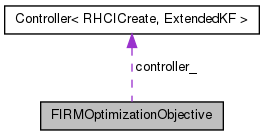
\includegraphics[width=336pt]{class_f_i_r_m_optimization_objective__coll__graph}
\end{center}
\end{figure}
\subsection*{\-Public \-Member \-Functions}
\begin{DoxyCompactItemize}
\item 
\hypertarget{class_f_i_r_m_optimization_objective_a230cd65e9c2c9d9d668eca55b9a9c537}{{\bfseries \-F\-I\-R\-M\-Optimization\-Objective} (const ompl\-::control\-::\-Space\-Information\-Ptr \&si)}\label{class_f_i_r_m_optimization_objective_a230cd65e9c2c9d9d668eca55b9a9c537}

\item 
\hypertarget{class_f_i_r_m_optimization_objective_a161f7e9f76e46cfb65a80109535c0bd1}{virtual ompl\-::base\-::\-Cost \hyperlink{class_f_i_r_m_optimization_objective_a161f7e9f76e46cfb65a80109535c0bd1}{motion\-Cost} (const ompl\-::base\-::\-State $\ast$s1, const ompl\-::base\-::\-State $\ast$s2)}\label{class_f_i_r_m_optimization_objective_a161f7e9f76e46cfb65a80109535c0bd1}

\begin{DoxyCompactList}\small\item\em \-Motion cost for this objective is defined as the sum of trace(covariance)for all intermediate states between {\itshape s1\/} and {\itshape s2\/}, using the method \-Space\-Information\-::distance(). \end{DoxyCompactList}\end{DoxyCompactItemize}
\subsection*{\-Protected \-Attributes}
\begin{DoxyCompactItemize}
\item 
\hypertarget{class_f_i_r_m_optimization_objective_ac8f288ac2a63ec1830889e2f146acbe6}{\hyperlink{class_controller}{\-Controller}$<$ \hyperlink{class_r_h_c_i_create}{\-R\-H\-C\-I\-Create}, \*
\hyperlink{class_extended_k_f}{\-Extended\-K\-F} $>$ {\bfseries controller\-\_\-}}\label{class_f_i_r_m_optimization_objective_ac8f288ac2a63ec1830889e2f146acbe6}

\end{DoxyCompactItemize}


\subsection{\-Detailed \-Description}
\-The cost to execute an edge i.\-e. going from some node \-A to some node \-B is defined as the \hyperlink{class_f_i_r_m}{\-F\-I\-R\-M} optimization objective. \-The cost is a measure of the uncertainty in the system (e.\-g. trace(covariance) for all intermediate states on the edge). \hyperlink{class_f_i_r_m}{\-F\-I\-R\-M} gives us paths that have the least uncertainty. 

\-The documentation for this class was generated from the following files\-:\begin{DoxyCompactItemize}
\item 
include/\-Optimization\-Objectives/\-F\-I\-R\-M\-Optimization\-Objective.\-h\item 
src/\-Optimization\-Objectives/\-F\-I\-R\-M\-Optimization\-Objective.\-cpp\end{DoxyCompactItemize}

\hypertarget{class_f_i_r_m_validity_checker}{\section{\-F\-I\-R\-M\-Validity\-Checker \-Class \-Reference}
\label{class_f_i_r_m_validity_checker}\index{\-F\-I\-R\-M\-Validity\-Checker@{\-F\-I\-R\-M\-Validity\-Checker}}
}
\subsection*{\-Public \-Types}
\begin{DoxyCompactItemize}
\item 
\hypertarget{class_f_i_r_m_validity_checker_ac646cd30f5012f2bd3298f3c93189867}{typedef \*
\-Observation\-Model\-Method\-::\-Observation\-Model\-Pointer {\bfseries \-Observation\-Model\-Pointer}}\label{class_f_i_r_m_validity_checker_ac646cd30f5012f2bd3298f3c93189867}

\item 
\hypertarget{class_f_i_r_m_validity_checker_af45d7b29a15e458b4bc5f7d6bf714ba2}{typedef \hyperlink{class_s_e2_belief_space_1_1_state_type}{\-S\-E2\-Belief\-Space\-::\-State\-Type} {\bfseries \-State\-Type}}\label{class_f_i_r_m_validity_checker_af45d7b29a15e458b4bc5f7d6bf714ba2}

\end{DoxyCompactItemize}
\subsection*{\-Public \-Member \-Functions}
\begin{DoxyCompactItemize}
\item 
\hyperlink{class_f_i_r_m_validity_checker_a6721f3a590c4ee967f57361aaba79b9d}{\-F\-I\-R\-M\-Validity\-Checker} (const ompl\-::base\-::\-Space\-Information\-Ptr \&si)
\item 
\hypertarget{class_f_i_r_m_validity_checker_a29fbd40e9a25430b7f5e296abe654f0b}{virtual bool {\bfseries is\-Valid} (const ompl\-::base\-::\-State $\ast$state) const }\label{class_f_i_r_m_validity_checker_a29fbd40e9a25430b7f5e296abe654f0b}

\end{DoxyCompactItemize}


\subsection{\-Constructor \& \-Destructor \-Documentation}
\hypertarget{class_f_i_r_m_validity_checker_a6721f3a590c4ee967f57361aaba79b9d}{\index{\-F\-I\-R\-M\-Validity\-Checker@{\-F\-I\-R\-M\-Validity\-Checker}!\-F\-I\-R\-M\-Validity\-Checker@{\-F\-I\-R\-M\-Validity\-Checker}}
\index{\-F\-I\-R\-M\-Validity\-Checker@{\-F\-I\-R\-M\-Validity\-Checker}!FIRMValidityChecker@{\-F\-I\-R\-M\-Validity\-Checker}}
\subsubsection[{\-F\-I\-R\-M\-Validity\-Checker}]{\setlength{\rightskip}{0pt plus 5cm}{\bf \-F\-I\-R\-M\-Validity\-Checker\-::\-F\-I\-R\-M\-Validity\-Checker} (
\begin{DoxyParamCaption}
\item[{const ompl\-::base\-::\-Space\-Information\-Ptr \&}]{si}
\end{DoxyParamCaption}
)\hspace{0.3cm}{\ttfamily  \mbox{[}inline\mbox{]}}}}\label{class_f_i_r_m_validity_checker_a6721f3a590c4ee967f57361aaba79b9d}
, observation\-Model\-\_\-(om) 
\begin{DoxyParams}{\-Parameters}
{\em si,\-Observation\-Model\-Pointer} & om \\
\hline
\end{DoxyParams}


\-The documentation for this class was generated from the following file\-:\begin{DoxyCompactItemize}
\item 
include/\-Validity\-Checkers/\-F\-I\-R\-M\-Validity\-Checker.\-h\end{DoxyCompactItemize}

\hypertarget{class_f_i_r_m_weight}{\section{\-F\-I\-R\-M\-Weight \-Class \-Reference}
\label{class_f_i_r_m_weight}\index{\-F\-I\-R\-M\-Weight@{\-F\-I\-R\-M\-Weight}}
}
\subsection*{\-Public \-Member \-Functions}
\begin{DoxyCompactItemize}
\item 
\hypertarget{class_f_i_r_m_weight_aaab8a3b391a0d39cbb777a4516433076}{{\bfseries \-F\-I\-R\-M\-Weight} (double cost=0, double success\-Probability=0, int controller\-I\-D=-\/1)}\label{class_f_i_r_m_weight_aaab8a3b391a0d39cbb777a4516433076}

\item 
\hypertarget{class_f_i_r_m_weight_a94ddb9e688e584d239161a2ee85c1085}{bool {\bfseries operator==} (const \hyperlink{class_f_i_r_m_weight}{\-F\-I\-R\-M\-Weight} \&w) const }\label{class_f_i_r_m_weight_a94ddb9e688e584d239161a2ee85c1085}

\item 
\hypertarget{class_f_i_r_m_weight_a8b7c01a43cada364fe0e0f471043bc1d}{const \hyperlink{class_f_i_r_m_weight}{\-F\-I\-R\-M\-Weight} \& {\bfseries operator=} (const \hyperlink{class_f_i_r_m_weight}{\-F\-I\-R\-M\-Weight} \&w)}\label{class_f_i_r_m_weight_a8b7c01a43cada364fe0e0f471043bc1d}

\item 
\hypertarget{class_f_i_r_m_weight_a3b342b0132221bbfa29e6f7eb3478bec}{\hyperlink{class_f_i_r_m_weight}{\-F\-I\-R\-M\-Weight} {\bfseries operator+} (const \hyperlink{class_f_i_r_m_weight}{\-F\-I\-R\-M\-Weight} \&w) const }\label{class_f_i_r_m_weight_a3b342b0132221bbfa29e6f7eb3478bec}

\item 
\hypertarget{class_f_i_r_m_weight_ab7c3de7f284f866bc1dc9a4b123e3c1c}{bool {\bfseries operator$<$} (const \hyperlink{class_f_i_r_m_weight}{\-F\-I\-R\-M\-Weight} \&w) const }\label{class_f_i_r_m_weight_ab7c3de7f284f866bc1dc9a4b123e3c1c}

\item 
\hypertarget{class_f_i_r_m_weight_a4fce79c475a69db5c001cb7771a42e97}{double {\bfseries get\-Cost} ()}\label{class_f_i_r_m_weight_a4fce79c475a69db5c001cb7771a42e97}

\item 
\hypertarget{class_f_i_r_m_weight_a75c60724969c1f443dec6b5817532f63}{void {\bfseries set\-Cost} (double c)}\label{class_f_i_r_m_weight_a75c60724969c1f443dec6b5817532f63}

\item 
\hypertarget{class_f_i_r_m_weight_af846636ead4117eee04ca622b0985c0f}{int {\bfseries get\-Controller\-I\-D} ()}\label{class_f_i_r_m_weight_af846636ead4117eee04ca622b0985c0f}

\item 
\hypertarget{class_f_i_r_m_weight_a7b19ae273970b48e156f79a2ef085b71}{void {\bfseries set\-Controller\-I\-D} (int id)}\label{class_f_i_r_m_weight_a7b19ae273970b48e156f79a2ef085b71}

\item 
\hypertarget{class_f_i_r_m_weight_a06b9e832fb364609e8d55fa9b4822dd9}{double {\bfseries get\-Success\-Probability} ()}\label{class_f_i_r_m_weight_a06b9e832fb364609e8d55fa9b4822dd9}

\item 
\hypertarget{class_f_i_r_m_weight_a464ea0457387ec93efa2342d27789d3e}{void {\bfseries set\-Success\-Probability} (double p)}\label{class_f_i_r_m_weight_a464ea0457387ec93efa2342d27789d3e}

\end{DoxyCompactItemize}
\subsection*{\-Protected \-Attributes}
\begin{DoxyCompactItemize}
\item 
\hypertarget{class_f_i_r_m_weight_a87d6234da67d63e0ee378f4817ba79b6}{double {\bfseries cost\-\_\-}}\label{class_f_i_r_m_weight_a87d6234da67d63e0ee378f4817ba79b6}

\item 
\hypertarget{class_f_i_r_m_weight_a11e740f671713d5859367648434f4b17}{double {\bfseries success\-Probability\-\_\-}}\label{class_f_i_r_m_weight_a11e740f671713d5859367648434f4b17}

\item 
\hypertarget{class_f_i_r_m_weight_a25113f31344f98970105be8c54a2f78d}{size\-\_\-t {\bfseries controller\-I\-D\-\_\-}}\label{class_f_i_r_m_weight_a25113f31344f98970105be8c54a2f78d}

\end{DoxyCompactItemize}


\-The documentation for this class was generated from the following file\-:\begin{DoxyCompactItemize}
\item 
include/\-Weight/\-F\-I\-R\-M\-Weight.\-h\end{DoxyCompactItemize}

\hypertarget{class_f_strategy}{\section{F\-Strategy$<$ Milestone $>$ Class Template Reference}
\label{class_f_strategy}\index{F\-Strategy$<$ Milestone $>$@{F\-Strategy$<$ Milestone $>$}}
}
\subsection*{Public Member Functions}
\begin{DoxyCompactItemize}
\item 
\hypertarget{class_f_strategy_acc3f67217f85960534aa23f5cf82c3c9}{\hyperlink{class_f_strategy_acc3f67217f85960534aa23f5cf82c3c9}{F\-Strategy} (double r, const std\-::shared\-\_\-ptr$<$ ompl\-::\-Nearest\-Neighbors$<$ Milestone $>$ $>$ \&nn)}\label{class_f_strategy_acc3f67217f85960534aa23f5cf82c3c9}

\begin{DoxyCompactList}\small\item\em Constructor takes the maximum number of nearest neighbors to return ({\itshape k}) and the nearest neighbors datastruture to use ({\itshape nn}) \end{DoxyCompactList}\item 
\hypertarget{class_f_strategy_a9e80a30f6c323e9ce704d29b17719b26}{void \hyperlink{class_f_strategy_a9e80a30f6c323e9ce704d29b17719b26}{set\-Nearest\-Neighbors} (const std\-::shared\-\_\-ptr$<$ ompl\-::\-Nearest\-Neighbors$<$ Milestone $>$ $>$ \&nn)}\label{class_f_strategy_a9e80a30f6c323e9ce704d29b17719b26}

\begin{DoxyCompactList}\small\item\em Set the nearest neighbors datastructure to use. \end{DoxyCompactList}\item 
\hypertarget{class_f_strategy_a88be84fef1b1d69a20acf7186d923255}{std\-::vector$<$ Milestone $>$ \& \hyperlink{class_f_strategy_a88be84fef1b1d69a20acf7186d923255}{operator()} (const Milestone \&m)}\label{class_f_strategy_a88be84fef1b1d69a20acf7186d923255}

\begin{DoxyCompactList}\small\item\em Given a milestone {\itshape m}, find the number of nearest neighbors connection attempts that should be made from it, according to the connection strategy. \end{DoxyCompactList}\end{DoxyCompactItemize}
\subsection*{Protected Attributes}
\begin{DoxyCompactItemize}
\item 
\hypertarget{class_f_strategy_a8a605936e6cfd37fd6c5c2d3c1f0c784}{double \hyperlink{class_f_strategy_a8a605936e6cfd37fd6c5c2d3c1f0c784}{radius\-\_\-}}\label{class_f_strategy_a8a605936e6cfd37fd6c5c2d3c1f0c784}

\begin{DoxyCompactList}\small\item\em Maximum distance to nearest neighbors to attempt to connect new milestones to. \end{DoxyCompactList}\item 
\hypertarget{class_f_strategy_ae35c08d00fb6489c36f401b13fce046a}{std\-::shared\-\_\-ptr\\*
$<$ ompl\-::\-Nearest\-Neighbors\\*
$<$ Milestone $>$ $>$ \hyperlink{class_f_strategy_ae35c08d00fb6489c36f401b13fce046a}{nn\-\_\-}}\label{class_f_strategy_ae35c08d00fb6489c36f401b13fce046a}

\begin{DoxyCompactList}\small\item\em Nearest neighbors data structure. \end{DoxyCompactList}\item 
\hypertarget{class_f_strategy_a3cd93caf2fd4d18f8033f02eeeab0b39}{std\-::vector$<$ Milestone $>$ \hyperlink{class_f_strategy_a3cd93caf2fd4d18f8033f02eeeab0b39}{neighbors\-\_\-}}\label{class_f_strategy_a3cd93caf2fd4d18f8033f02eeeab0b39}

\begin{DoxyCompactList}\small\item\em Scratch space for storing k-\/nearest neighbors. \end{DoxyCompactList}\end{DoxyCompactItemize}


The documentation for this class was generated from the following file\-:\begin{DoxyCompactItemize}
\item 
include/\-Connection\-Strategy/F\-Strategy.\-h\end{DoxyCompactItemize}

\hypertarget{class_gaussian_valid_belief_sampler}{\section{\-Gaussian\-Valid\-Belief\-Sampler \-Class \-Reference}
\label{class_gaussian_valid_belief_sampler}\index{\-Gaussian\-Valid\-Belief\-Sampler@{\-Gaussian\-Valid\-Belief\-Sampler}}
}


\-Generate valid samples using the \-Gaussian sampling strategy.  




{\ttfamily \#include $<$\-Gaussian\-Valid\-Belief\-Sampler.\-h$>$}

\subsection*{\-Public \-Types}
\begin{DoxyCompactItemize}
\item 
\hypertarget{class_gaussian_valid_belief_sampler_a61a22b17254765f0c32940bb1d118473}{typedef \*
\-Observation\-Model\-Method\-::\-Observation\-Model\-Pointer {\bfseries \-Observation\-Model\-Pointer}}\label{class_gaussian_valid_belief_sampler_a61a22b17254765f0c32940bb1d118473}

\end{DoxyCompactItemize}
\subsection*{\-Public \-Member \-Functions}
\begin{DoxyCompactItemize}
\item 
\hypertarget{class_gaussian_valid_belief_sampler_ae3c0e5503ddc85cc2943d3fda5ca1247}{\hyperlink{class_gaussian_valid_belief_sampler_ae3c0e5503ddc85cc2943d3fda5ca1247}{\-Gaussian\-Valid\-Belief\-Sampler} (const \hyperlink{classfirm_1_1_space_information}{firm\-::\-Space\-Information} $\ast$si)}\label{class_gaussian_valid_belief_sampler_ae3c0e5503ddc85cc2943d3fda5ca1247}

\begin{DoxyCompactList}\small\item\em \-Constructor. \end{DoxyCompactList}\item 
\hypertarget{class_gaussian_valid_belief_sampler_a70901adff599cc2219f7269568bad91d}{virtual bool {\bfseries sample} (ompl\-::base\-::\-State $\ast$state)}\label{class_gaussian_valid_belief_sampler_a70901adff599cc2219f7269568bad91d}

\item 
\hypertarget{class_gaussian_valid_belief_sampler_a0e08191a299ce7ddc48f2e316c9fdd65}{virtual bool {\bfseries sample\-Near} (ompl\-::base\-::\-State $\ast$state, const ompl\-::base\-::\-State $\ast$near, const double distance)}\label{class_gaussian_valid_belief_sampler_a0e08191a299ce7ddc48f2e316c9fdd65}

\item 
\hypertarget{class_gaussian_valid_belief_sampler_a3e6bb843f415b78742efcebbc9657ed0}{double \hyperlink{class_gaussian_valid_belief_sampler_a3e6bb843f415b78742efcebbc9657ed0}{get\-Std\-Dev} (void) const }\label{class_gaussian_valid_belief_sampler_a3e6bb843f415b78742efcebbc9657ed0}

\begin{DoxyCompactList}\small\item\em \-Get the standard deviation used when sampling. \end{DoxyCompactList}\item 
\hypertarget{class_gaussian_valid_belief_sampler_ab0beca356924545e0cb27292495995a5}{void \hyperlink{class_gaussian_valid_belief_sampler_ab0beca356924545e0cb27292495995a5}{set\-Std\-Dev} (double stddev)}\label{class_gaussian_valid_belief_sampler_ab0beca356924545e0cb27292495995a5}

\begin{DoxyCompactList}\small\item\em \-Set the standard deviation to use when sampling. \end{DoxyCompactList}\end{DoxyCompactItemize}
\subsection*{\-Protected \-Member \-Functions}
\begin{DoxyCompactItemize}
\item 
bool \hyperlink{class_gaussian_valid_belief_sampler_a87de26ec14b44eb5946d6c27b06416c6}{is\-Observable} (ompl\-::base\-::\-State $\ast$state)
\end{DoxyCompactItemize}
\subsection*{\-Protected \-Attributes}
\begin{DoxyCompactItemize}
\item 
\hypertarget{class_gaussian_valid_belief_sampler_ac479e9335daee424ce105648b068a018}{ompl\-::base\-::\-State\-Sampler\-Ptr \hyperlink{class_gaussian_valid_belief_sampler_ac479e9335daee424ce105648b068a018}{sampler\-\_\-}}\label{class_gaussian_valid_belief_sampler_ac479e9335daee424ce105648b068a018}

\begin{DoxyCompactList}\small\item\em \-The sampler to build upon. \end{DoxyCompactList}\item 
\hypertarget{class_gaussian_valid_belief_sampler_a46c46db4485e69a1c6ba5c65e175a8d3}{double \hyperlink{class_gaussian_valid_belief_sampler_a46c46db4485e69a1c6ba5c65e175a8d3}{stddev\-\_\-}}\label{class_gaussian_valid_belief_sampler_a46c46db4485e69a1c6ba5c65e175a8d3}

\begin{DoxyCompactList}\small\item\em \-The standard deviation to use in the sampling process. \end{DoxyCompactList}\end{DoxyCompactItemize}


\subsection{\-Detailed \-Description}
\-Generate valid samples using the \-Gaussian sampling strategy. 

\subsection{\-Member \-Function \-Documentation}
\hypertarget{class_gaussian_valid_belief_sampler_a87de26ec14b44eb5946d6c27b06416c6}{\index{\-Gaussian\-Valid\-Belief\-Sampler@{\-Gaussian\-Valid\-Belief\-Sampler}!is\-Observable@{is\-Observable}}
\index{is\-Observable@{is\-Observable}!GaussianValidBeliefSampler@{\-Gaussian\-Valid\-Belief\-Sampler}}
\subsubsection[{is\-Observable}]{\setlength{\rightskip}{0pt plus 5cm}bool {\bf \-Gaussian\-Valid\-Belief\-Sampler\-::is\-Observable} (
\begin{DoxyParamCaption}
\item[{ompl\-::base\-::\-State $\ast$}]{state}
\end{DoxyParamCaption}
)\hspace{0.3cm}{\ttfamily  \mbox{[}protected\mbox{]}}}}\label{class_gaussian_valid_belief_sampler_a87de26ec14b44eb5946d6c27b06416c6}
void set\-Observation\-Model(\-Observation\-Model\-Pointer om) \{ observation\-Model\-\_\- = om; \} brief \-Checks if the sample is observable i.\-e. \-If it can observe sufficient landmarks \-Ideally, observability check should be performed in the filter instead of obs model 

\-The documentation for this class was generated from the following files\-:\begin{DoxyCompactItemize}
\item 
include/\-Samplers/\-Gaussian\-Valid\-Belief\-Sampler.\-h\item 
src/\-Samplers/\-Gaussian\-Valid\-Belief\-Sampler.\-cpp\end{DoxyCompactItemize}

\hypertarget{class_g_l_widget}{\section{G\-L\-Widget Class Reference}
\label{class_g_l_widget}\index{G\-L\-Widget@{G\-L\-Widget}}
}


Inheritance diagram for G\-L\-Widget\-:\nopagebreak
\begin{figure}[H]
\begin{center}
\leavevmode
\includegraphics[width=148pt]{class_g_l_widget__inherit__graph}
\end{center}
\end{figure}


Collaboration diagram for G\-L\-Widget\-:\nopagebreak
\begin{figure}[H]
\begin{center}
\leavevmode
\includegraphics[width=148pt]{class_g_l_widget__coll__graph}
\end{center}
\end{figure}
\subsection*{Public Types}
\begin{DoxyCompactItemize}
\item 
\hypertarget{class_g_l_widget_a5ee4f2222a72d52e211cbe47bfb74807}{typedef \hyperlink{class_visualizer}{Visualizer} {\bfseries Display}}\label{class_g_l_widget_a5ee4f2222a72d52e211cbe47bfb74807}

\end{DoxyCompactItemize}
\subsection*{Public Slots}
\begin{DoxyCompactItemize}
\item 
\hypertarget{class_g_l_widget_a133cbc2c72a274f0175edc01f7b3d807}{void {\bfseries draw\-Axes} (bool)}\label{class_g_l_widget_a133cbc2c72a274f0175edc01f7b3d807}

\item 
\hypertarget{class_g_l_widget_a485193a89a6340023e5bc7256fa8b0b7}{void {\bfseries save\-Snapshot} ()}\label{class_g_l_widget_a485193a89a6340023e5bc7256fa8b0b7}

\item 
\hypertarget{class_g_l_widget_a459a667a4f8aafdcf420ede286a25b2e}{void {\bfseries Change\-Mode} (int)}\label{class_g_l_widget_a459a667a4f8aafdcf420ede286a25b2e}

\end{DoxyCompactItemize}
\subsection*{Public Member Functions}
\begin{DoxyCompactItemize}
\item 
\hypertarget{class_g_l_widget_ab79c391c86de1ffb76f6950b49d82c0c}{{\bfseries G\-L\-Widget} (Q\-Widget $\ast$parent=0)}\label{class_g_l_widget_ab79c391c86de1ffb76f6950b49d82c0c}

\item 
\hypertarget{class_g_l_widget_ade3142625c1bfda0576e419b176cf8b1}{Q\-Size {\bfseries minimum\-Size\-Hint} () const }\label{class_g_l_widget_ade3142625c1bfda0576e419b176cf8b1}

\item 
\hypertarget{class_g_l_widget_a57698bc426052845b43a135a13540154}{Q\-Size {\bfseries size\-Hint} () const }\label{class_g_l_widget_a57698bc426052845b43a135a13540154}

\item 
\hypertarget{class_g_l_widget_aa46294065b5d7cce0595792401ad7b12}{void {\bfseries reset\-Cam} ()}\label{class_g_l_widget_aa46294065b5d7cce0595792401ad7b12}

\item 
\hypertarget{class_g_l_widget_af243f58b80dffdd66c3ad1fa26d0122a}{void {\bfseries move\-Cam} (double \-\_\-delta)}\label{class_g_l_widget_af243f58b80dffdd66c3ad1fa26d0122a}

\item 
\hypertarget{class_g_l_widget_a807139ab40c3c79de628af8d3cfb6e71}{void {\bfseries strafe\-Cam} (double \-\_\-delta)}\label{class_g_l_widget_a807139ab40c3c79de628af8d3cfb6e71}

\item 
\hypertarget{class_g_l_widget_ab0b5ab19881e8b9a1e1b748b08613dce}{void {\bfseries zoom\-Cam} (double \-\_\-delta)}\label{class_g_l_widget_ab0b5ab19881e8b9a1e1b748b08613dce}

\end{DoxyCompactItemize}
\subsection*{Public Attributes}
\begin{DoxyCompactItemize}
\item 
\hypertarget{class_g_l_widget_a20f2af9cd6308b71c95e8a96857dc46d}{bool {\bfseries m\-\_\-draw\-Axes}}\label{class_g_l_widget_a20f2af9cd6308b71c95e8a96857dc46d}

\end{DoxyCompactItemize}
\subsection*{Protected Member Functions}
\begin{DoxyCompactItemize}
\item 
\hypertarget{class_g_l_widget_a7fab13e8cc9fc0730ca54c08b2c923a7}{void {\bfseries initialize\-G\-L} ()}\label{class_g_l_widget_a7fab13e8cc9fc0730ca54c08b2c923a7}

\item 
\hypertarget{class_g_l_widget_a640b5570cb2b37724fd5b58a77339c5e}{void {\bfseries paint\-G\-L} ()}\label{class_g_l_widget_a640b5570cb2b37724fd5b58a77339c5e}

\item 
\hypertarget{class_g_l_widget_ac0d2a8ecf60907a81c0d73475d851025}{void {\bfseries resize\-G\-L} (int width, int height)}\label{class_g_l_widget_ac0d2a8ecf60907a81c0d73475d851025}

\item 
\hypertarget{class_g_l_widget_ab144cc8064c1bbf6d0ef0646ca0bd06c}{void {\bfseries mouse\-Press\-Event} (Q\-Mouse\-Event $\ast$event)}\label{class_g_l_widget_ab144cc8064c1bbf6d0ef0646ca0bd06c}

\item 
\hypertarget{class_g_l_widget_a9043bac13d6f0a5307ea5c7f9b3caa50}{void {\bfseries mouse\-Move\-Event} (Q\-Mouse\-Event $\ast$event)}\label{class_g_l_widget_a9043bac13d6f0a5307ea5c7f9b3caa50}

\item 
\hypertarget{class_g_l_widget_a0495fe7afc77e7782111f5816405abc0}{void {\bfseries mouse\-Double\-Click\-Event} (Q\-Mouse\-Event $\ast$event)}\label{class_g_l_widget_a0495fe7afc77e7782111f5816405abc0}

\item 
\hypertarget{class_g_l_widget_a3fc170fb9be74bc3e771b6356bf981b2}{void {\bfseries save\-Frame} ()}\label{class_g_l_widget_a3fc170fb9be74bc3e771b6356bf981b2}

\item 
\hypertarget{class_g_l_widget_a068f6ece9170b92f3b54741b3ff8df9f}{void {\bfseries save\-Image} (Q\-String \&)}\label{class_g_l_widget_a068f6ece9170b92f3b54741b3ff8df9f}

\end{DoxyCompactItemize}
\subsection*{Private Attributes}
\begin{DoxyCompactItemize}
\item 
\hypertarget{class_g_l_widget_aa66efb8d767894fcb141913ba9dbae11}{arma\-::colvec {\bfseries m\-\_\-cam\-Pos}}\label{class_g_l_widget_aa66efb8d767894fcb141913ba9dbae11}

\item 
\hypertarget{class_g_l_widget_a3050be303596d9558380eb45188a6a33}{arma\-::colvec {\bfseries m\-\_\-cam\-At}}\label{class_g_l_widget_a3050be303596d9558380eb45188a6a33}

\item 
\hypertarget{class_g_l_widget_ab58c3a83eaad7958ef32a0e38312dfa0}{double {\bfseries m\-\_\-cam\-Zoom}}\label{class_g_l_widget_ab58c3a83eaad7958ef32a0e38312dfa0}

\item 
\hypertarget{class_g_l_widget_a4911eae2c543a1dbd35a2f21d4da1dd5}{string {\bfseries m\-\_\-filename}}\label{class_g_l_widget_a4911eae2c543a1dbd35a2f21d4da1dd5}

\item 
\hypertarget{class_g_l_widget_ae2e31a41f9a824cab2ebb039efdf8e6f}{double {\bfseries m\-\_\-long}}\label{class_g_l_widget_ae2e31a41f9a824cab2ebb039efdf8e6f}

\item 
\hypertarget{class_g_l_widget_a8246562eab0ffa67f6f3aaae4208b7f6}{double {\bfseries m\-\_\-lat}}\label{class_g_l_widget_a8246562eab0ffa67f6f3aaae4208b7f6}

\item 
\hypertarget{class_g_l_widget_aac1f587db6a0e2112fe4c21fc449f470}{Q\-Point {\bfseries m\-\_\-last\-Pos}}\label{class_g_l_widget_aac1f587db6a0e2112fe4c21fc449f470}

\item 
\hypertarget{class_g_l_widget_a89b241a362a60322f411bd0fbdccfb60}{bool {\bfseries m\-\_\-view}}\label{class_g_l_widget_a89b241a362a60322f411bd0fbdccfb60}

\item 
\hypertarget{class_g_l_widget_a4d466e74fd00b09d4474e8c6163b7094}{Q\-String {\bfseries m\-\_\-snapshot\-Path}}\label{class_g_l_widget_a4d466e74fd00b09d4474e8c6163b7094}

\item 
\hypertarget{class_g_l_widget_a593d0bcfcb11c4c0c43f75bc35f4e4b1}{Q\-String {\bfseries m\-\_\-frame\-Path}}\label{class_g_l_widget_a593d0bcfcb11c4c0c43f75bc35f4e4b1}

\end{DoxyCompactItemize}


The documentation for this class was generated from the following files\-:\begin{DoxyCompactItemize}
\item 
include/\-Visualization/G\-L\-Widget.\-h\item 
src/\-Visualization/G\-L\-Widget.\-cpp\end{DoxyCompactItemize}

\hypertarget{class_kalman_filter_method}{\section{\-Kalman\-Filter\-Method \-Class \-Reference}
\label{class_kalman_filter_method}\index{\-Kalman\-Filter\-Method@{\-Kalman\-Filter\-Method}}
}


\-Inheritance diagram for \-Kalman\-Filter\-Method\-:
\nopagebreak
\begin{figure}[H]
\begin{center}
\leavevmode
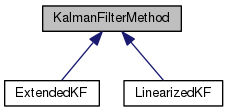
\includegraphics[width=242pt]{class_kalman_filter_method__inherit__graph}
\end{center}
\end{figure}
\subsection*{\-Public \-Member \-Functions}
\begin{DoxyCompactItemize}
\item 
\hypertarget{class_kalman_filter_method_afbea7fdb6e6faffd74de8ee647b97a02}{{\bfseries \-Kalman\-Filter\-Method} (firm\-::\-Space\-Information\-::\-Space\-Information\-Ptr si)}\label{class_kalman_filter_method_afbea7fdb6e6faffd74de8ee647b97a02}

\item 
\hypertarget{class_kalman_filter_method_aed467f00719c58d7be5458f8f99511d9}{\-Motion\-Model\-Pointer {\bfseries get\-Motion\-Model\-Pointer} ()}\label{class_kalman_filter_method_aed467f00719c58d7be5458f8f99511d9}

\item 
\hypertarget{class_kalman_filter_method_a7f2542d72d92f1e44cf4d0cdcaec02b8}{void {\bfseries set\-Motion\-Model\-Pointeer} (const \-Motion\-Model\-Pointer \&mm)}\label{class_kalman_filter_method_a7f2542d72d92f1e44cf4d0cdcaec02b8}

\item 
\hypertarget{class_kalman_filter_method_aa93f7e7e297eb337cc1fda8ae46763cc}{\-Observation\-Model\-Pointer {\bfseries get\-Observation\-Model\-Pointer} ()}\label{class_kalman_filter_method_aa93f7e7e297eb337cc1fda8ae46763cc}

\item 
\hypertarget{class_kalman_filter_method_a4b966a487acbbdda0f145be9a1da03d5}{void {\bfseries set\-Observation\-Model\-Pointer} (const \-Observation\-Model\-Pointer \&om)}\label{class_kalman_filter_method_a4b966a487acbbdda0f145be9a1da03d5}

\item 
\hypertarget{class_kalman_filter_method_ae8d8c8f2eeaca1a556cfc655d1897ce5}{virtual void {\bfseries \-Predict} (const ompl\-::base\-::\-State $\ast$belief, const ompl\-::control\-::\-Control $\ast$control, const \hyperlink{class_linear_system}{\-Linear\-System} \&ls, ompl\-::base\-::\-State $\ast$predicted\-State, const bool is\-Construction=false)=0}\label{class_kalman_filter_method_ae8d8c8f2eeaca1a556cfc655d1897ce5}

\item 
\hypertarget{class_kalman_filter_method_aac4f9c1f1a79821898891f2c13aa5cfc}{virtual void {\bfseries \-Update} (const ompl\-::base\-::\-State $\ast$belief, const \-Observation\-Type \&obs, const \hyperlink{class_linear_system}{\-Linear\-System} \&ls, ompl\-::base\-::\-State $\ast$updated\-State, const bool is\-Construction=false)=0}\label{class_kalman_filter_method_aac4f9c1f1a79821898891f2c13aa5cfc}

\item 
\hypertarget{class_kalman_filter_method_a8a13cf9a962588fbd3441726b7b95e77}{virtual void {\bfseries \-Evolve} (const ompl\-::base\-::\-State $\ast$belief, const ompl\-::control\-::\-Control $\ast$control, const \-Observation\-Type \&obs, const \hyperlink{class_linear_system}{\-Linear\-System} \&ls\-Pred, const \hyperlink{class_linear_system}{\-Linear\-System} \&ls\-Update, ompl\-::base\-::\-State $\ast$evolved\-State, const bool is\-Construction=false)=0}\label{class_kalman_filter_method_a8a13cf9a962588fbd3441726b7b95e77}

\item 
\hypertarget{class_kalman_filter_method_a8f9d8ae8cf4e3bd0138d731bd2539441}{virtual arma\-::mat {\bfseries compute\-Stationary\-Covariance} (const \hyperlink{class_linear_system}{\-Linear\-System} \&ls)=0}\label{class_kalman_filter_method_a8f9d8ae8cf4e3bd0138d731bd2539441}

\end{DoxyCompactItemize}
\subsection*{\-Protected \-Attributes}
\begin{DoxyCompactItemize}
\item 
\hypertarget{class_kalman_filter_method_a9a2355339d83656f5db7c86a60d12822}{firm\-::\-Space\-Information\-::\-Space\-Information\-Ptr {\bfseries si\-\_\-}}\label{class_kalman_filter_method_a9a2355339d83656f5db7c86a60d12822}

\item 
\hypertarget{class_kalman_filter_method_a5969ade2e4d4f70a1cccc2f2f2bf4bb3}{\-Motion\-Model\-Pointer {\bfseries motion\-Model\-\_\-}}\label{class_kalman_filter_method_a5969ade2e4d4f70a1cccc2f2f2bf4bb3}

\item 
\hypertarget{class_kalman_filter_method_a43191b745846715c66854634ba58e85c}{\-Observation\-Model\-Pointer {\bfseries observation\-Model\-\_\-}}\label{class_kalman_filter_method_a43191b745846715c66854634ba58e85c}

\end{DoxyCompactItemize}


\-The documentation for this class was generated from the following file\-:\begin{DoxyCompactItemize}
\item 
include/\-Filters/\-Kalman\-Filter\-Method.\-h\end{DoxyCompactItemize}

\hypertarget{class_linearized_k_f}{\section{\-Linearized\-K\-F \-Class \-Reference}
\label{class_linearized_k_f}\index{\-Linearized\-K\-F@{\-Linearized\-K\-F}}
}


\-A \-Linearized \-Kalman \-Filter.  




{\ttfamily \#include $<$\-Linearized\-K\-F.\-h$>$}



\-Inheritance diagram for \-Linearized\-K\-F\-:\nopagebreak
\begin{figure}[H]
\begin{center}
\leavevmode
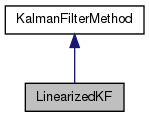
\includegraphics[width=184pt]{class_linearized_k_f__inherit__graph}
\end{center}
\end{figure}


\-Collaboration diagram for \-Linearized\-K\-F\-:\nopagebreak
\begin{figure}[H]
\begin{center}
\leavevmode
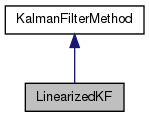
\includegraphics[width=184pt]{class_linearized_k_f__coll__graph}
\end{center}
\end{figure}
\subsection*{\-Public \-Types}
\begin{DoxyCompactItemize}
\item 
\hypertarget{class_linearized_k_f_a7c538be0fa27f880c2272d6b1fbe8729}{typedef \*
\-Motion\-Model\-Method\-::\-Control\-Type {\bfseries \-Control\-Type}}\label{class_linearized_k_f_a7c538be0fa27f880c2272d6b1fbe8729}

\item 
\hypertarget{class_linearized_k_f_a068ecc6782388590cba62370670585d1}{typedef \*
\hyperlink{class_s_e2_belief_space}{\-Motion\-Model\-Method\-::\-Space\-Type} {\bfseries \-Space\-Type}}\label{class_linearized_k_f_a068ecc6782388590cba62370670585d1}

\item 
\hypertarget{class_linearized_k_f_aab4a87264c8e70b665298697e4a49a02}{typedef \*
\hyperlink{class_s_e2_belief_space_1_1_state_type}{\-Motion\-Model\-Method\-::\-State\-Type} {\bfseries \-State\-Type}}\label{class_linearized_k_f_aab4a87264c8e70b665298697e4a49a02}

\item 
\hypertarget{class_linearized_k_f_a66feb5ecffc79354460e8bd3d431ff12}{typedef \*
\-Observation\-Model\-Method\-::\-Observation\-Type {\bfseries \-Observation\-Type}}\label{class_linearized_k_f_a66feb5ecffc79354460e8bd3d431ff12}

\item 
\hypertarget{class_linearized_k_f_a2673ebedf419ec686789f03d94c3307f}{typedef \*
\-Motion\-Model\-Method\-::\-Motion\-Model\-Pointer {\bfseries \-Motion\-Model\-Pointer}}\label{class_linearized_k_f_a2673ebedf419ec686789f03d94c3307f}

\item 
\hypertarget{class_linearized_k_f_a885fd5b62c570da6e5eaf1f1fc33d542}{typedef \*
\-Observation\-Model\-Method\-::\-Observation\-Model\-Pointer {\bfseries \-Observation\-Model\-Pointer}}\label{class_linearized_k_f_a885fd5b62c570da6e5eaf1f1fc33d542}

\end{DoxyCompactItemize}
\subsection*{\-Public \-Member \-Functions}
\begin{DoxyCompactItemize}
\item 
\hypertarget{class_linearized_k_f_a65e7448c5edd6d4130ce7bd1ec6e0cc5}{\hyperlink{class_linearized_k_f_a65e7448c5edd6d4130ce7bd1ec6e0cc5}{\-Linearized\-K\-F} ()}\label{class_linearized_k_f_a65e7448c5edd6d4130ce7bd1ec6e0cc5}

\begin{DoxyCompactList}\small\item\em \-Constructor. \end{DoxyCompactList}\item 
\hypertarget{class_linearized_k_f_a904ee8b6525d0358dc1ee426eb19be9b}{\hyperlink{class_linearized_k_f_a904ee8b6525d0358dc1ee426eb19be9b}{\-Linearized\-K\-F} (const firm\-::\-Space\-Information\-::\-Space\-Information\-Ptr si)}\label{class_linearized_k_f_a904ee8b6525d0358dc1ee426eb19be9b}

\begin{DoxyCompactList}\small\item\em \-Constructor. \end{DoxyCompactList}\item 
\hypertarget{class_linearized_k_f_a62bda6a7234592bad9e227d45788cf51}{void \hyperlink{class_linearized_k_f_a62bda6a7234592bad9e227d45788cf51}{\-Predict} (const ompl\-::base\-::\-State $\ast$belief, const ompl\-::control\-::\-Control $\ast$control, const \hyperlink{class_linear_system}{\-Linear\-System} \&ls, ompl\-::base\-::\-State $\ast$predicted\-State)}\label{class_linearized_k_f_a62bda6a7234592bad9e227d45788cf51}

\begin{DoxyCompactList}\small\item\em \-Gets as input belief and control, returns predicted belief if control were to be applied to the robot. \-Also called the \-Prior. \end{DoxyCompactList}\item 
\hypertarget{class_linearized_k_f_abb67e01d9e14a67de60aaa6cdde56552}{void \hyperlink{class_linearized_k_f_abb67e01d9e14a67de60aaa6cdde56552}{\-Update} (const ompl\-::base\-::\-State $\ast$belief, const \-Observation\-Type \&obs, const \hyperlink{class_linear_system}{\-Linear\-System} \&ls, ompl\-::base\-::\-State $\ast$updated\-State)}\label{class_linearized_k_f_abb67e01d9e14a67de60aaa6cdde56552}

\begin{DoxyCompactList}\small\item\em \-Gets as input belief and observation, returns the updated state of the robot. \-Also called the \-Posterior. \end{DoxyCompactList}\item 
\hypertarget{class_linearized_k_f_a9de5546e208e7c49ce443c94625cbebc}{void \hyperlink{class_linearized_k_f_a9de5546e208e7c49ce443c94625cbebc}{\-Evolve} (const ompl\-::base\-::\-State $\ast$belief, const ompl\-::control\-::\-Control $\ast$control, const \-Observation\-Type \&obs, const \hyperlink{class_linear_system}{\-Linear\-System} \&ls\-Pred, const \hyperlink{class_linear_system}{\-Linear\-System} \&ls\-Update, ompl\-::base\-::\-State $\ast$evolved\-State)}\label{class_linearized_k_f_a9de5546e208e7c49ce443c94625cbebc}

\begin{DoxyCompactList}\small\item\em \-Evolves the robot's belief on the input control, previous state and new observation. \-It first calls predict and then update. \end{DoxyCompactList}\item 
\hypertarget{class_linearized_k_f_addb9369d36e6d9fcb49668f8ca19ad97}{arma\-::mat \hyperlink{class_linearized_k_f_addb9369d36e6d9fcb49668f8ca19ad97}{compute\-Stationary\-Covariance} (const \hyperlink{class_linear_system}{\-Linear\-System} \&ls)}\label{class_linearized_k_f_addb9369d36e6d9fcb49668f8ca19ad97}

\begin{DoxyCompactList}\small\item\em \-Compute the covariance for a given linear system. \-A linear system describes a robot's state at a point in an open loop trajectory. \-Helps to understand the expected uncertainty at a point in the trajectory. \end{DoxyCompactList}\end{DoxyCompactItemize}


\subsection{\-Detailed \-Description}
\-A \-Linearized \-Kalman \-Filter. 

\-The documentation for this class was generated from the following files\-:\begin{DoxyCompactItemize}
\item 
include/\-Filters/\-Linearized\-K\-F.\-h\item 
src/\-Filters/\-Linearized\-K\-F.\-cpp\end{DoxyCompactItemize}

\hypertarget{class_linear_system}{\section{\-Linear\-System \-Class \-Reference}
\label{class_linear_system}\index{\-Linear\-System@{\-Linear\-System}}
}
\subsection*{\-Public \-Types}
\begin{DoxyCompactItemize}
\item 
\hypertarget{class_linear_system_a6e2a2cea01eb7d624ebddbd35da87391}{typedef \*
\hyperlink{class_s_e2_belief_space}{\-Motion\-Model\-Method\-::\-Space\-Type} {\bfseries \-Space\-Type}}\label{class_linear_system_a6e2a2cea01eb7d624ebddbd35da87391}

\item 
\hypertarget{class_linear_system_a18a7ea2657a1fbca633a2dfb92fbdfcc}{typedef \*
\hyperlink{class_s_e2_belief_space_1_1_state_type}{\-Motion\-Model\-Method\-::\-State\-Type} {\bfseries \-State\-Type}}\label{class_linear_system_a18a7ea2657a1fbca633a2dfb92fbdfcc}

\item 
\hypertarget{class_linear_system_a45a2dc5d393c50bc2d475cd9f4ff1db0}{typedef \*
\-Motion\-Model\-Method\-::\-Motion\-Model\-Pointer {\bfseries \-Motion\-Model\-Pointer}}\label{class_linear_system_a45a2dc5d393c50bc2d475cd9f4ff1db0}

\item 
\hypertarget{class_linear_system_a239819b1a3b5554c9b1ffbe669492b6e}{typedef \*
\-Observation\-Model\-Method\-::\-Observation\-Model\-Pointer {\bfseries \-Observation\-Model\-Pointer}}\label{class_linear_system_a239819b1a3b5554c9b1ffbe669492b6e}

\item 
\hypertarget{class_linear_system_ac89acd811aeb518081df96fb3904b176}{typedef arma\-::mat {\bfseries \-Control\-Type}}\label{class_linear_system_ac89acd811aeb518081df96fb3904b176}

\item 
\hypertarget{class_linear_system_abdf29233ee72fe498a01fe4bae172efd}{typedef arma\-::mat {\bfseries \-Motion\-Noise\-Type}}\label{class_linear_system_abdf29233ee72fe498a01fe4bae172efd}

\item 
\hypertarget{class_linear_system_a331ff229efb09e79a474ab87f246b0c6}{typedef arma\-::mat {\bfseries \-Observation\-Type}}\label{class_linear_system_a331ff229efb09e79a474ab87f246b0c6}

\item 
\hypertarget{class_linear_system_ab9c0d62af5d52a64f6e51c3236ec92c8}{typedef arma\-::mat {\bfseries \-Obs\-Noise\-Type}}\label{class_linear_system_ab9c0d62af5d52a64f6e51c3236ec92c8}

\item 
\hypertarget{class_linear_system_ad3aad199efe5346e1fad4b05f47a9cad}{typedef arma\-::mat {\bfseries \-Motion\-Jacobian\-Type}}\label{class_linear_system_ad3aad199efe5346e1fad4b05f47a9cad}

\item 
\hypertarget{class_linear_system_ab7d8a6454e58308029700805c02693a5}{typedef arma\-::mat {\bfseries \-Obs\-Jacobian\-Type}}\label{class_linear_system_ab7d8a6454e58308029700805c02693a5}

\end{DoxyCompactItemize}
\subsection*{\-Public \-Member \-Functions}
\begin{DoxyCompactItemize}
\item 
\hypertarget{class_linear_system_a6f05277076a4302dbcfa9646232871dc}{{\bfseries \-Linear\-System} (const ompl\-::base\-::\-State $\ast$state, const ompl\-::control\-::\-Control $\ast$control, \-Motion\-Model\-Pointer motion\-Model, \-Observation\-Model\-Pointer observation\-Model)}\label{class_linear_system_a6f05277076a4302dbcfa9646232871dc}

\item 
\hypertarget{class_linear_system_a428c800b858ed6c6d63230c64e470208}{{\bfseries \-Linear\-System} (const ompl\-::base\-::\-State $\ast$state, const ompl\-::control\-::\-Control $\ast$control, const \-Observation\-Type \&obs, \-Motion\-Model\-Pointer motion\-Model, \-Observation\-Model\-Pointer observation\-Model)}\label{class_linear_system_a428c800b858ed6c6d63230c64e470208}

\item 
\hypertarget{class_linear_system_a7d556441c0f68f6ccfdde32b72f888b6}{ompl\-::base\-::\-State $\ast$ {\bfseries get\-X} ()}\label{class_linear_system_a7d556441c0f68f6ccfdde32b72f888b6}

\item 
\hypertarget{class_linear_system_aa9b7cdb3f9e09902fbe9b1d65d932edb}{arma\-::mat {\bfseries get\-A} () const }\label{class_linear_system_aa9b7cdb3f9e09902fbe9b1d65d932edb}

\item 
\hypertarget{class_linear_system_af1a0b99cb2b4e30eb61b1bee328fb0bd}{arma\-::mat {\bfseries get\-B} () const }\label{class_linear_system_af1a0b99cb2b4e30eb61b1bee328fb0bd}

\item 
\hypertarget{class_linear_system_aaadd9d063ecdb4afb67ae4522cf921a7}{arma\-::mat {\bfseries get\-G} () const }\label{class_linear_system_aaadd9d063ecdb4afb67ae4522cf921a7}

\item 
\hypertarget{class_linear_system_ab95733398800308c2e69522d37f2a005}{arma\-::mat {\bfseries get\-Q} () const }\label{class_linear_system_ab95733398800308c2e69522d37f2a005}

\item 
\hypertarget{class_linear_system_a678fe164168013e7a4a4fc97e6716fa6}{arma\-::mat {\bfseries get\-H} () const }\label{class_linear_system_a678fe164168013e7a4a4fc97e6716fa6}

\item 
\hypertarget{class_linear_system_a4b69f2e4c7b6144c6abb8abf725ce063}{arma\-::mat {\bfseries get\-M} () const }\label{class_linear_system_a4b69f2e4c7b6144c6abb8abf725ce063}

\item 
\hypertarget{class_linear_system_aaad4f742dcb61f776d5de952977a745e}{arma\-::mat {\bfseries get\-R} () const }\label{class_linear_system_aaad4f742dcb61f776d5de952977a745e}

\end{DoxyCompactItemize}


\-The documentation for this class was generated from the following file\-:\begin{DoxyCompactItemize}
\item 
include/\-Linear\-System/\-Linear\-System.\-h\end{DoxyCompactItemize}

\hypertarget{class_motion_model_method}{\section{\-Motion\-Model\-Method \-Class \-Reference}
\label{class_motion_model_method}\index{\-Motion\-Model\-Method@{\-Motion\-Model\-Method}}
}


\-Inheritance diagram for \-Motion\-Model\-Method\-:
\nopagebreak
\begin{figure}[H]
\begin{center}
\leavevmode
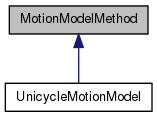
\includegraphics[width=190pt]{class_motion_model_method__inherit__graph}
\end{center}
\end{figure}
\subsection*{\-Public \-Types}
\begin{DoxyCompactItemize}
\item 
\hypertarget{class_motion_model_method_a3d2d250cadace8b47d5eca028a2220e4}{typedef arma\-::colvec {\bfseries \-Control\-Type}}\label{class_motion_model_method_a3d2d250cadace8b47d5eca028a2220e4}

\item 
\hypertarget{class_motion_model_method_aecf04875853e2ecbebc66eb720adc63b}{typedef arma\-::colvec {\bfseries \-Noise\-Type}}\label{class_motion_model_method_aecf04875853e2ecbebc66eb720adc63b}

\item 
\hypertarget{class_motion_model_method_ada60008f50c4ec1f48956bf99fa846ed}{typedef \hyperlink{class_s_e2_belief_space}{\-S\-E2\-Belief\-Space} {\bfseries \-Space\-Type}}\label{class_motion_model_method_ada60008f50c4ec1f48956bf99fa846ed}

\item 
\hypertarget{class_motion_model_method_a15b3c3801cb64f85bfff7d088d276d91}{typedef \hyperlink{class_s_e2_belief_space_1_1_state_type}{\-Space\-Type\-::\-State\-Type} {\bfseries \-State\-Type}}\label{class_motion_model_method_a15b3c3801cb64f85bfff7d088d276d91}

\item 
\hypertarget{class_motion_model_method_a2c6d9dc15fc37a1d5079f72c4114ebed}{typedef arma\-::mat {\bfseries \-Jacobian\-Type}}\label{class_motion_model_method_a2c6d9dc15fc37a1d5079f72c4114ebed}

\item 
\hypertarget{class_motion_model_method_a94a8bd757d2cfb258a47cdd69079e506}{typedef boost\-::shared\-\_\-ptr\*
$<$ \hyperlink{class_motion_model_method}{\-Motion\-Model\-Method} $>$ {\bfseries \-Motion\-Model\-Pointer}}\label{class_motion_model_method_a94a8bd757d2cfb258a47cdd69079e506}

\end{DoxyCompactItemize}
\subsection*{\-Public \-Member \-Functions}
\begin{DoxyCompactItemize}
\item 
\hypertarget{class_motion_model_method_ae5ef4bfae24bc1674db07f785eb7d6f4}{{\bfseries \-Motion\-Model\-Method} (ompl\-::control\-::\-Space\-Information\-Ptr si, int n\-Dim=0)}\label{class_motion_model_method_ae5ef4bfae24bc1674db07f785eb7d6f4}

\item 
\hypertarget{class_motion_model_method_aa15c21f81b71cfe8c65224bbdfba61d8}{void {\bfseries set\-Time\-Step} (double time\-Step)}\label{class_motion_model_method_aa15c21f81b71cfe8c65224bbdfba61d8}

\item 
\hypertarget{class_motion_model_method_a9fafbf79b4ea570819e01050dadf4826}{virtual void {\bfseries \-Evolve} (const ompl\-::base\-::\-State $\ast$state, const ompl\-::control\-::\-Control $\ast$control, const \-Noise\-Type \&w, ompl\-::base\-::\-State $\ast$result)=0}\label{class_motion_model_method_a9fafbf79b4ea570819e01050dadf4826}

\item 
\hypertarget{class_motion_model_method_a6ec853871652bfa2c4fdad2c46e81e44}{virtual void {\bfseries generate\-Open\-Loop\-Controls} (const ompl\-::base\-::\-State $\ast$start\-State, const ompl\-::base\-::\-State $\ast$end\-State, std\-::vector$<$ ompl\-::control\-::\-Control $\ast$ $>$ \&open\-Loop\-Controls)=0}\label{class_motion_model_method_a6ec853871652bfa2c4fdad2c46e81e44}

\item 
\hypertarget{class_motion_model_method_a036e2254bcae3730fe157419f9cf9c19}{virtual \-Noise\-Type {\bfseries generate\-Noise} (const ompl\-::base\-::\-State $\ast$state, const ompl\-::control\-::\-Control $\ast$control)=0}\label{class_motion_model_method_a036e2254bcae3730fe157419f9cf9c19}

\item 
\hypertarget{class_motion_model_method_af1429b7c54c0b6bdde9e6b8272bbb50e}{virtual \-Jacobian\-Type {\bfseries get\-State\-Jacobian} (const ompl\-::base\-::\-State $\ast$state, const ompl\-::control\-::\-Control $\ast$control, const \-Noise\-Type \&w)=0}\label{class_motion_model_method_af1429b7c54c0b6bdde9e6b8272bbb50e}

\item 
\hypertarget{class_motion_model_method_aac2be89931926f5883fd4e0ec0b7a073}{virtual \-Jacobian\-Type {\bfseries get\-Control\-Jacobian} (const ompl\-::base\-::\-State $\ast$state, const ompl\-::control\-::\-Control $\ast$control, const \-Noise\-Type \&w)=0}\label{class_motion_model_method_aac2be89931926f5883fd4e0ec0b7a073}

\item 
\hypertarget{class_motion_model_method_adefbf482a8d6d409b262cb1af014026a}{virtual \-Jacobian\-Type {\bfseries get\-Noise\-Jacobian} (const ompl\-::base\-::\-State $\ast$state, const ompl\-::control\-::\-Control $\ast$control, const \-Noise\-Type \&w)=0}\label{class_motion_model_method_adefbf482a8d6d409b262cb1af014026a}

\item 
\hypertarget{class_motion_model_method_a559dc48932d5aca3215e3f24e29680ce}{virtual arma\-::mat {\bfseries process\-Noise\-Covariance} (const ompl\-::base\-::\-State $\ast$state, const ompl\-::control\-::\-Control $\ast$control)=0}\label{class_motion_model_method_a559dc48932d5aca3215e3f24e29680ce}

\item 
\hypertarget{class_motion_model_method_a4002e8e3bb3af13d56bc162b655a1543}{virtual ompl\-::control\-::\-Control $\ast$ {\bfseries get\-Zero\-Control} ()}\label{class_motion_model_method_a4002e8e3bb3af13d56bc162b655a1543}

\item 
\hypertarget{class_motion_model_method_a56d9a853b4ec8158c4c9016614c86a9f}{virtual const \-Noise\-Type \& {\bfseries get\-Zero\-Noise} ()}\label{class_motion_model_method_a56d9a853b4ec8158c4c9016614c86a9f}

\item 
\hypertarget{class_motion_model_method_ad0012e93feba030fa8e9a47a18c6ff0e}{virtual const size\-\_\-t {\bfseries control\-Dim} ()}\label{class_motion_model_method_ad0012e93feba030fa8e9a47a18c6ff0e}

\item 
\hypertarget{class_motion_model_method_a86ef6178a4d438fde83f1c3f110ad2b4}{virtual double {\bfseries get\-Timestep\-Size} ()}\label{class_motion_model_method_a86ef6178a4d438fde83f1c3f110ad2b4}

\item 
\hypertarget{class_motion_model_method_a924d7bb8eb665d12181c3755e831bc50}{arma\-::colvec {\bfseries \-O\-M\-P\-L2\-A\-R\-M\-A} (const ompl\-::control\-::\-Control $\ast$control)}\label{class_motion_model_method_a924d7bb8eb665d12181c3755e831bc50}

\item 
\hypertarget{class_motion_model_method_af473fd665c4fa562143beef5733db523}{void {\bfseries \-A\-R\-M\-A2\-O\-M\-P\-L} (arma\-::colvec u, ompl\-::control\-::\-Control $\ast$control)}\label{class_motion_model_method_af473fd665c4fa562143beef5733db523}

\end{DoxyCompactItemize}
\subsection*{\-Protected \-Attributes}
\begin{DoxyCompactItemize}
\item 
\hypertarget{class_motion_model_method_a7410df94d1231268c431dd73f2e5338d}{ompl\-::control\-::\-Space\-Information\-Ptr {\bfseries si\-\_\-}}\label{class_motion_model_method_a7410df94d1231268c431dd73f2e5338d}

\item 
\hypertarget{class_motion_model_method_a6d76506c342c3bf089eb548c531e2105}{const unsigned int {\bfseries state\-Dim\-\_\-}}\label{class_motion_model_method_a6d76506c342c3bf089eb548c531e2105}

\item 
\hypertarget{class_motion_model_method_ab9b45acbafce1f4c873ee7095bc49964}{const unsigned int {\bfseries control\-Dim\-\_\-}}\label{class_motion_model_method_ab9b45acbafce1f4c873ee7095bc49964}

\item 
\hypertarget{class_motion_model_method_ae5e55aa39c0d819c3e9afffefa3d5b08}{ompl\-::control\-::\-Control $\ast$ {\bfseries zero\-Control\-\_\-}}\label{class_motion_model_method_ae5e55aa39c0d819c3e9afffefa3d5b08}

\item 
\hypertarget{class_motion_model_method_a47725ad490fdc510cdc38838165b27c6}{const int {\bfseries noise\-Dim\-\_\-}}\label{class_motion_model_method_a47725ad490fdc510cdc38838165b27c6}

\item 
\hypertarget{class_motion_model_method_ac5b0a8829ec75b20d78deff84f71cbb5}{\-Noise\-Type {\bfseries zero\-Noise\-\_\-}}\label{class_motion_model_method_ac5b0a8829ec75b20d78deff84f71cbb5}

\item 
\hypertarget{class_motion_model_method_a482972cd2ec0bec4b42137811e1d0446}{double {\bfseries dt\-\_\-}}\label{class_motion_model_method_a482972cd2ec0bec4b42137811e1d0446}

\end{DoxyCompactItemize}


\-The documentation for this class was generated from the following file\-:\begin{DoxyCompactItemize}
\item 
include/\-Motion\-Models/\-Motion\-Model\-Method.\-h\end{DoxyCompactItemize}

\hypertarget{class_my_window}{\section{My\-Window Class Reference}
\label{class_my_window}\index{My\-Window@{My\-Window}}
}


Inheritance diagram for My\-Window\-:\nopagebreak
\begin{figure}[H]
\begin{center}
\leavevmode
\includegraphics[width=144pt]{class_my_window__inherit__graph}
\end{center}
\end{figure}


Collaboration diagram for My\-Window\-:\nopagebreak
\begin{figure}[H]
\begin{center}
\leavevmode
\includegraphics[width=217pt]{class_my_window__coll__graph}
\end{center}
\end{figure}
\subsection*{Public Member Functions}
\begin{DoxyCompactItemize}
\item 
\hypertarget{class_my_window_a42c07be4c6795c9a1858b63d28b30eb0}{void {\bfseries reset\-Camera} ()}\label{class_my_window_a42c07be4c6795c9a1858b63d28b30eb0}

\end{DoxyCompactItemize}
\subsection*{Protected Member Functions}
\begin{DoxyCompactItemize}
\item 
\hypertarget{class_my_window_aa773620138509c878d8ebe27961b5e9c}{void {\bfseries key\-Press\-Event} (Q\-Key\-Event $\ast$event)}\label{class_my_window_aa773620138509c878d8ebe27961b5e9c}

\end{DoxyCompactItemize}
\subsection*{Private Slots}
\begin{DoxyCompactItemize}
\item 
\hypertarget{class_my_window_a06c416f5d60e88b134f22149cdbfd185}{void {\bfseries simulate} ()}\label{class_my_window_a06c416f5d60e88b134f22149cdbfd185}

\end{DoxyCompactItemize}
\subsection*{Private Attributes}
\begin{DoxyCompactItemize}
\item 
\hypertarget{class_my_window_a42ef11e52721811070d715142a9f2b04}{Q\-Timer {\bfseries timer\-\_\-}}\label{class_my_window_a42ef11e52721811070d715142a9f2b04}

\item 
\hypertarget{class_my_window_a82841f4322a0a0975d71ad021bd4a0df}{\hyperlink{class_g_l_widget}{G\-L\-Widget} $\ast$ {\bfseries gl\-Widget\-\_\-}}\label{class_my_window_a82841f4322a0a0975d71ad021bd4a0df}

\end{DoxyCompactItemize}


The documentation for this class was generated from the following files\-:\begin{DoxyCompactItemize}
\item 
include/\-Visualization/Window.\-h\item 
src/\-Visualization/Window.\-cpp\end{DoxyCompactItemize}

\hypertarget{class_observation_model_method}{\section{\-Observation\-Model\-Method \-Class \-Reference}
\label{class_observation_model_method}\index{\-Observation\-Model\-Method@{\-Observation\-Model\-Method}}
}


\-Inheritance diagram for \-Observation\-Model\-Method\-:\nopagebreak
\begin{figure}[H]
\begin{center}
\leavevmode
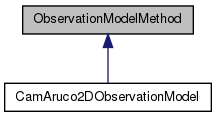
\includegraphics[width=234pt]{class_observation_model_method__inherit__graph}
\end{center}
\end{figure}
\subsection*{\-Public \-Types}
\begin{DoxyCompactItemize}
\item 
\hypertarget{class_observation_model_method_af5a5953c0f7b82691d36f353ed08aa03}{typedef arma\-::colvec {\bfseries \-Observation\-Type}}\label{class_observation_model_method_af5a5953c0f7b82691d36f353ed08aa03}

\item 
\hypertarget{class_observation_model_method_a380b1d02a13fa85f2a4d8610b648d446}{typedef arma\-::colvec {\bfseries \-Noise\-Type}}\label{class_observation_model_method_a380b1d02a13fa85f2a4d8610b648d446}

\item 
\hypertarget{class_observation_model_method_a1c83d0c9794c0316818c0ee87fba4a24}{typedef arma\-::mat {\bfseries \-Obs\-To\-State\-Jacobian\-Type}}\label{class_observation_model_method_a1c83d0c9794c0316818c0ee87fba4a24}

\item 
\hypertarget{class_observation_model_method_ac1a379fcac7d5d5d67391362eb91c252}{typedef arma\-::mat {\bfseries \-Obs\-To\-Noise\-Jacobian\-Type}}\label{class_observation_model_method_ac1a379fcac7d5d5d67391362eb91c252}

\item 
\hypertarget{class_observation_model_method_ad119ee691daccc6a1410de7a18a93b7f}{typedef boost\-::shared\-\_\-ptr\*
$<$ \hyperlink{class_observation_model_method}{\-Observation\-Model\-Method} $>$ {\bfseries \-Observation\-Model\-Pointer}}\label{class_observation_model_method_ad119ee691daccc6a1410de7a18a93b7f}

\end{DoxyCompactItemize}
\subsection*{\-Public \-Member \-Functions}
\begin{DoxyCompactItemize}
\item 
\hypertarget{class_observation_model_method_ace82963106629ded581fd8b43c4a0a6b}{{\bfseries \-Observation\-Model\-Method} (int n\-Dim=0)}\label{class_observation_model_method_ace82963106629ded581fd8b43c4a0a6b}

\item 
virtual \-Observation\-Type \hyperlink{class_observation_model_method_af1a30aad975576ae8f16042a8ee8276b}{get\-Observation} (const ompl\-::base\-::\-State $\ast$state, bool is\-Simulation)=0
\item 
\hypertarget{class_observation_model_method_a9d10ee1be836ef4d406c85b35efd72d8}{virtual \-Observation\-Type {\bfseries get\-Observation\-Prediction} (const ompl\-::base\-::\-State $\ast$state, const \-Observation\-Type \&\-Zg)=0}\label{class_observation_model_method_a9d10ee1be836ef4d406c85b35efd72d8}

\item 
\hypertarget{class_observation_model_method_acd2e16185fbfd1c25b22b77e52acc936}{virtual \-Obs\-To\-State\-Jacobian\-Type {\bfseries get\-Observation\-Jacobian} (const ompl\-::base\-::\-State $\ast$state, const \-Noise\-Type \&v, const \-Observation\-Type \&z)=0}\label{class_observation_model_method_acd2e16185fbfd1c25b22b77e52acc936}

\item 
\hypertarget{class_observation_model_method_af53dcf93c40fd8589e84a3cfe48a0c7e}{virtual \-Obs\-To\-Noise\-Jacobian\-Type {\bfseries get\-Noise\-Jacobian} (const ompl\-::base\-::\-State $\ast$state, const \-Noise\-Type \&v, const \-Observation\-Type \&z)=0}\label{class_observation_model_method_af53dcf93c40fd8589e84a3cfe48a0c7e}

\item 
\hypertarget{class_observation_model_method_a359c3b1473a12dcbaa73f7e63d7cf202}{virtual \-Observation\-Type {\bfseries compute\-Innovation} (const ompl\-::base\-::\-State $\ast$predicted\-State, const \-Observation\-Type \&\-Zg)=0}\label{class_observation_model_method_a359c3b1473a12dcbaa73f7e63d7cf202}

\item 
\hypertarget{class_observation_model_method_af0ef30992e4ecd8adc81bed96e6d6663}{virtual arma\-::mat {\bfseries get\-Observation\-Noise\-Covariance} (const ompl\-::base\-::\-State $\ast$state, const \-Observation\-Type \&z)=0}\label{class_observation_model_method_af0ef30992e4ecd8adc81bed96e6d6663}

\item 
\hypertarget{class_observation_model_method_a351bcd27e192c0cc6f07650c3d9beb70}{virtual bool {\bfseries is\-State\-Observable} (const ompl\-::base\-::\-State $\ast$state)=0}\label{class_observation_model_method_a351bcd27e192c0cc6f07650c3d9beb70}

\item 
\hypertarget{class_observation_model_method_a86809e73a6e01b37f82fe822bd500b7b}{virtual const \-Noise\-Type {\bfseries get\-Zero\-Noise} ()}\label{class_observation_model_method_a86809e73a6e01b37f82fe822bd500b7b}

\end{DoxyCompactItemize}
\subsection*{\-Public \-Attributes}
\begin{DoxyCompactItemize}
\item 
\hypertarget{class_observation_model_method_a183fbeb021b40c30e29239b1c1b895bf}{arma\-::colvec {\bfseries eta\-Phi\-\_\-}}\label{class_observation_model_method_a183fbeb021b40c30e29239b1c1b895bf}

\item 
\hypertarget{class_observation_model_method_a7cd6d5c8235775f6227d3ee5458927db}{arma\-::colvec {\bfseries eta\-D\-\_\-}}\label{class_observation_model_method_a7cd6d5c8235775f6227d3ee5458927db}

\item 
\hypertarget{class_observation_model_method_a126bab071775905203dee38c709444c3}{arma\-::colvec {\bfseries sigma\-\_\-}}\label{class_observation_model_method_a126bab071775905203dee38c709444c3}

\end{DoxyCompactItemize}
\subsection*{\-Private \-Attributes}
\begin{DoxyCompactItemize}
\item 
\hypertarget{class_observation_model_method_adf0334680c9f2f49320c1d584ae9d1b3}{const int {\bfseries noise\-Dim\-\_\-}}\label{class_observation_model_method_adf0334680c9f2f49320c1d584ae9d1b3}

\item 
\hypertarget{class_observation_model_method_a30517a6bfae555908e82880f9d23492c}{const \-Noise\-Type {\bfseries zero\-Noise\-\_\-}}\label{class_observation_model_method_a30517a6bfae555908e82880f9d23492c}

\end{DoxyCompactItemize}


\subsection{\-Member \-Function \-Documentation}
\hypertarget{class_observation_model_method_af1a30aad975576ae8f16042a8ee8276b}{\index{\-Observation\-Model\-Method@{\-Observation\-Model\-Method}!get\-Observation@{get\-Observation}}
\index{get\-Observation@{get\-Observation}!ObservationModelMethod@{\-Observation\-Model\-Method}}
\subsubsection[{get\-Observation}]{\setlength{\rightskip}{0pt plus 5cm}virtual \-Observation\-Type {\bf \-Observation\-Model\-Method\-::get\-Observation} (
\begin{DoxyParamCaption}
\item[{const ompl\-::base\-::\-State $\ast$}]{state, }
\item[{bool}]{is\-Simulation}
\end{DoxyParamCaption}
)\hspace{0.3cm}{\ttfamily  \mbox{[}pure virtual\mbox{]}}}}\label{class_observation_model_method_af1a30aad975576ae8f16042a8ee8276b}
z = h(x,v) get the observation for a given configuration. 1. is\-Simulation= true , corrupted by noise from a given distribution 2. is\-Simulation=false , noise free obs 

\-Implemented in \hyperlink{class_cam_aruco2_d_observation_model_a244fd43dca1734b68bf1379b2be285d2}{\-Cam\-Aruco2\-D\-Observation\-Model}.



\-The documentation for this class was generated from the following file\-:\begin{DoxyCompactItemize}
\item 
include/\-Observation\-Models/\-Observation\-Model\-Method.\-h\end{DoxyCompactItemize}

\input{class_o_g_l_display}
\input{struct_o_g_l_display_1_1_o_g_l_feedback_edge}
\input{struct_ti_xml_string_1_1_rep}
\hypertarget{class_r_h_c_i_create}{\section{\-R\-H\-C\-I\-Create \-Class \-Reference}
\label{class_r_h_c_i_create}\index{\-R\-H\-C\-I\-Create@{\-R\-H\-C\-I\-Create}}
}


\-Inheritance diagram for \-R\-H\-C\-I\-Create\-:
\nopagebreak
\begin{figure}[H]
\begin{center}
\leavevmode
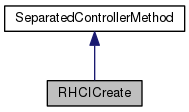
\includegraphics[width=214pt]{class_r_h_c_i_create__inherit__graph}
\end{center}
\end{figure}


\-Collaboration diagram for \-R\-H\-C\-I\-Create\-:
\nopagebreak
\begin{figure}[H]
\begin{center}
\leavevmode
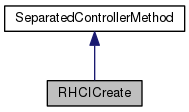
\includegraphics[width=214pt]{class_r_h_c_i_create__coll__graph}
\end{center}
\end{figure}
\subsection*{\-Public \-Types}
\begin{DoxyCompactItemize}
\item 
\hypertarget{class_r_h_c_i_create_a11c369848f9c90605af210dcbcfb0194}{typedef \*
\-Separated\-Controller\-Method\-::\-Control\-Type {\bfseries \-Control\-Type}}\label{class_r_h_c_i_create_a11c369848f9c90605af210dcbcfb0194}

\item 
\hypertarget{class_r_h_c_i_create_a662339ec07c14710db2903785224c183}{typedef \*
\-Motion\-Model\-Method\-::\-Motion\-Model\-Pointer {\bfseries \-Motion\-Model\-Pointer}}\label{class_r_h_c_i_create_a662339ec07c14710db2903785224c183}

\end{DoxyCompactItemize}
\subsection*{\-Public \-Member \-Functions}
\begin{DoxyCompactItemize}
\item 
\hypertarget{class_r_h_c_i_create_ae7a6a7c12aadfa3787c331658d257860}{{\bfseries \-R\-H\-C\-I\-Create} (ompl\-::base\-::\-State $\ast$goal, const std\-::vector$<$ ompl\-::base\-::\-State $\ast$ $>$ \&nominal\-Xs, const std\-::vector$<$ ompl\-::control\-::\-Control $\ast$ $>$ \&nominal\-Us, const std\-::vector$<$ \hyperlink{class_linear_system}{\-Linear\-System} $>$ \&linear\-Systems, const \-Motion\-Model\-Pointer mm)}\label{class_r_h_c_i_create_ae7a6a7c12aadfa3787c331658d257860}

\item 
\hypertarget{class_r_h_c_i_create_a098e194144edb28b252e97d78200f078}{virtual ompl\-::control\-::\-Control $\ast$ {\bfseries generate\-Feedback\-Control} (const ompl\-::base\-::\-State $\ast$state, const size\-\_\-t \&\-\_\-t=0)}\label{class_r_h_c_i_create_a098e194144edb28b252e97d78200f078}

\end{DoxyCompactItemize}
\subsection*{\-Static \-Public \-Member \-Functions}
\begin{DoxyCompactItemize}
\item 
\hypertarget{class_r_h_c_i_create_a6fa2c185a82c7ec346e9a4a81f5158c3}{static void {\bfseries set\-Control\-Queue\-Size} (const int queue\-Size)}\label{class_r_h_c_i_create_a6fa2c185a82c7ec346e9a4a81f5158c3}

\item 
\hypertarget{class_r_h_c_i_create_a08e9bd17083a978c6b5cd142bca84460}{static void {\bfseries set\-Turn\-Only\-Distance} (const double turn\-Dist)}\label{class_r_h_c_i_create_a08e9bd17083a978c6b5cd142bca84460}

\end{DoxyCompactItemize}


\-The documentation for this class was generated from the following files\-:\begin{DoxyCompactItemize}
\item 
include/\-Separated\-Controllers/\-R\-H\-C\-I\-Create.\-h\item 
src/\-Separated\-Controllers/\-R\-H\-C\-I\-Create.\-cpp\end{DoxyCompactItemize}

\hypertarget{class_s_e2_belief_space}{\section{\-S\-E2\-Belief\-Space \-Class \-Reference}
\label{class_s_e2_belief_space}\index{\-S\-E2\-Belief\-Space@{\-S\-E2\-Belief\-Space}}
}
\subsection*{\-Classes}
\begin{DoxyCompactItemize}
\item 
class \hyperlink{class_s_e2_belief_space_1_1_state_type}{\-State\-Type}
\begin{DoxyCompactList}\small\item\em \-A belief in \-S\-E(2)\-: (x, y, yaw, covariance) \end{DoxyCompactList}\end{DoxyCompactItemize}
\subsection*{\-Public \-Member \-Functions}
\begin{DoxyCompactItemize}
\item 
void \hyperlink{class_s_e2_belief_space_a5802f054e3cbb060fd96a42398d4ff6d}{set\-Bounds} (const \-Real\-Vector\-Bounds \&bounds)
\item 
const \-Real\-Vector\-Bounds \& \hyperlink{class_s_e2_belief_space_a05aba6731aec5046e99df18c7c8603f0}{get\-Bounds} (void) const 
\item 
\hypertarget{class_s_e2_belief_space_a58efacef9a9413925bd48d0da71b7886}{virtual \-State $\ast$ {\bfseries alloc\-State} (void) const }\label{class_s_e2_belief_space_a58efacef9a9413925bd48d0da71b7886}

\item 
\hypertarget{class_s_e2_belief_space_a64eeb0fb62f8ed174c95604e22b759cd}{virtual void {\bfseries copy\-State} (\-State $\ast$destination, const \-State $\ast$source) const }\label{class_s_e2_belief_space_a64eeb0fb62f8ed174c95604e22b759cd}

\item 
\hypertarget{class_s_e2_belief_space_a0dedcfe61f35ab4eed2f997615856a89}{virtual void {\bfseries free\-State} (\-State $\ast$state) const }\label{class_s_e2_belief_space_a0dedcfe61f35ab4eed2f997615856a89}

\item 
\hypertarget{class_s_e2_belief_space_a96f20d1a29f25fddbabe0c56ff408006}{virtual double {\bfseries distance} (const \-State $\ast$state1, const \-State $\ast$state2)}\label{class_s_e2_belief_space_a96f20d1a29f25fddbabe0c56ff408006}

\item 
\hypertarget{class_s_e2_belief_space_a6d840d9e02dfd15b410e4671a7e94623}{void {\bfseries get\-Relative\-State} (const \-State $\ast$from, const \-State $\ast$to, \-State $\ast$state)}\label{class_s_e2_belief_space_a6d840d9e02dfd15b410e4671a7e94623}

\item 
\hypertarget{class_s_e2_belief_space_a6efc6e19ffd078fe38ede1c2120bea2f}{void {\bfseries print\-Belief\-State} (const \-State $\ast$state)}\label{class_s_e2_belief_space_a6efc6e19ffd078fe38ede1c2120bea2f}

\end{DoxyCompactItemize}


\subsection{\-Member \-Function \-Documentation}
\hypertarget{class_s_e2_belief_space_a05aba6731aec5046e99df18c7c8603f0}{\index{\-S\-E2\-Belief\-Space@{\-S\-E2\-Belief\-Space}!get\-Bounds@{get\-Bounds}}
\index{get\-Bounds@{get\-Bounds}!SE2BeliefSpace@{\-S\-E2\-Belief\-Space}}
\subsubsection[{get\-Bounds}]{\setlength{\rightskip}{0pt plus 5cm}const \-Real\-Vector\-Bounds\& {\bf \-S\-E2\-Belief\-Space\-::get\-Bounds} (
\begin{DoxyParamCaption}
\item[{void}]{}
\end{DoxyParamCaption}
) const\hspace{0.3cm}{\ttfamily  \mbox{[}inline\mbox{]}}}}\label{class_s_e2_belief_space_a05aba6731aec5046e99df18c7c8603f0}
 \hypertarget{class_s_e2_belief_space_a5802f054e3cbb060fd96a42398d4ff6d}{\index{\-S\-E2\-Belief\-Space@{\-S\-E2\-Belief\-Space}!set\-Bounds@{set\-Bounds}}
\index{set\-Bounds@{set\-Bounds}!SE2BeliefSpace@{\-S\-E2\-Belief\-Space}}
\subsubsection[{set\-Bounds}]{\setlength{\rightskip}{0pt plus 5cm}void {\bf \-S\-E2\-Belief\-Space\-::set\-Bounds} (
\begin{DoxyParamCaption}
\item[{const \-Real\-Vector\-Bounds \&}]{bounds}
\end{DoxyParamCaption}
)\hspace{0.3cm}{\ttfamily  \mbox{[}inline\mbox{]}}}}\label{class_s_e2_belief_space_a5802f054e3cbb060fd96a42398d4ff6d}
 

\-The documentation for this class was generated from the following files\-:\begin{DoxyCompactItemize}
\item 
include/\-Spaces/\-S\-E2\-Belief\-Space.\-h\item 
src/\-Spaces/\-S\-E2\-Belief\-Space.\-cpp\end{DoxyCompactItemize}

\hypertarget{class_separated_controller_method}{\section{\-Separated\-Controller\-Method \-Class \-Reference}
\label{class_separated_controller_method}\index{\-Separated\-Controller\-Method@{\-Separated\-Controller\-Method}}
}


\-Inheritance diagram for \-Separated\-Controller\-Method\-:
\nopagebreak
\begin{figure}[H]
\begin{center}
\leavevmode
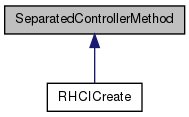
\includegraphics[width=214pt]{class_separated_controller_method__inherit__graph}
\end{center}
\end{figure}
\subsection*{\-Public \-Types}
\begin{DoxyCompactItemize}
\item 
\hypertarget{class_separated_controller_method_af037a93db2d2c315265bf3df79231ebc}{typedef \*
\hyperlink{class_s_e2_belief_space}{\-Motion\-Model\-Method\-::\-Space\-Type} {\bfseries \-Space\-Type}}\label{class_separated_controller_method_af037a93db2d2c315265bf3df79231ebc}

\item 
\hypertarget{class_separated_controller_method_a69af9f746a9cb93e9807eee8df538258}{typedef \*
\hyperlink{class_s_e2_belief_space_1_1_state_type}{\-Motion\-Model\-Method\-::\-State\-Type} {\bfseries \-State\-Type}}\label{class_separated_controller_method_a69af9f746a9cb93e9807eee8df538258}

\item 
\hypertarget{class_separated_controller_method_a969bf25e6b70eb1b1ae3adf2ae3bb813}{typedef \*
\-Motion\-Model\-Method\-::\-Control\-Type {\bfseries \-Control\-Type}}\label{class_separated_controller_method_a969bf25e6b70eb1b1ae3adf2ae3bb813}

\item 
\hypertarget{class_separated_controller_method_a108499f2f2ba359907aba634d6812854}{typedef \*
\-Observation\-Model\-Method\-::\-Observation\-Type {\bfseries \-Observation\-Type}}\label{class_separated_controller_method_a108499f2f2ba359907aba634d6812854}

\item 
\hypertarget{class_separated_controller_method_a2ebae1dd9ad6568e6cf14fe82808a68d}{typedef \*
\-Motion\-Model\-Method\-::\-Motion\-Model\-Pointer {\bfseries \-Motion\-Model\-Pointer}}\label{class_separated_controller_method_a2ebae1dd9ad6568e6cf14fe82808a68d}

\item 
\hypertarget{class_separated_controller_method_a68eeb1e05fd5b6bff498c0e77fb4e4df}{typedef arma\-::mat {\bfseries \-Cost\-Type}}\label{class_separated_controller_method_a68eeb1e05fd5b6bff498c0e77fb4e4df}

\item 
\hypertarget{class_separated_controller_method_a419460dff807103eed3f1043e9fcbb7c}{typedef arma\-::mat {\bfseries \-Gain\-Type}}\label{class_separated_controller_method_a419460dff807103eed3f1043e9fcbb7c}

\end{DoxyCompactItemize}
\subsection*{\-Public \-Member \-Functions}
\begin{DoxyCompactItemize}
\item 
\hypertarget{class_separated_controller_method_a972840f44e5e93b293bba9b2a5a2f8db}{{\bfseries \-Separated\-Controller\-Method} (ompl\-::base\-::\-State $\ast$goal, const std\-::vector$<$ ompl\-::base\-::\-State $\ast$ $>$ \&nominal\-Xs, const std\-::vector$<$ ompl\-::control\-::\-Control $\ast$ $>$ \&nominal\-Us, const std\-::vector$<$ \hyperlink{class_linear_system}{\-Linear\-System} $>$ \&linear\-Systems, const \-Motion\-Model\-Pointer mm)}\label{class_separated_controller_method_a972840f44e5e93b293bba9b2a5a2f8db}

\item 
\hypertarget{class_separated_controller_method_a1a69b57856c903834a4f353ebd561749}{virtual ompl\-::control\-::\-Control $\ast$ {\bfseries generate\-Feedback\-Control} (const ompl\-::base\-::\-State $\ast$state, const size\-\_\-t \&\-\_\-t=0)=0}\label{class_separated_controller_method_a1a69b57856c903834a4f353ebd561749}

\end{DoxyCompactItemize}
\subsection*{\-Protected \-Attributes}
\begin{DoxyCompactItemize}
\item 
\hypertarget{class_separated_controller_method_ac5fa2b730632d0367986649d664e7640}{ompl\-::base\-::\-State $\ast$ {\bfseries goal\-\_\-}}\label{class_separated_controller_method_ac5fa2b730632d0367986649d664e7640}

\item 
\hypertarget{class_separated_controller_method_a77c380ed4f2af1ca89f3856cd8ad6435}{std\-::vector$<$ ompl\-::base\-::\-State $\ast$ $>$ {\bfseries nominal\-Xs\-\_\-}}\label{class_separated_controller_method_a77c380ed4f2af1ca89f3856cd8ad6435}

\item 
\hypertarget{class_separated_controller_method_a822729a081bfc3438c4632ad99d418d4}{std\-::vector\*
$<$ ompl\-::control\-::\-Control $\ast$ $>$ {\bfseries nominal\-Us\-\_\-}}\label{class_separated_controller_method_a822729a081bfc3438c4632ad99d418d4}

\item 
\hypertarget{class_separated_controller_method_a977cb3b7a14a072d10b4529875737ebd}{std\-::vector$<$ \hyperlink{class_linear_system}{\-Linear\-System} $>$ {\bfseries linear\-Systems\-\_\-}}\label{class_separated_controller_method_a977cb3b7a14a072d10b4529875737ebd}

\item 
\hypertarget{class_separated_controller_method_ae23167d348557320997ecb359bb82403}{\-Motion\-Model\-Pointer {\bfseries motion\-Model\-\_\-}}\label{class_separated_controller_method_ae23167d348557320997ecb359bb82403}

\end{DoxyCompactItemize}


\-The documentation for this class was generated from the following file\-:\begin{DoxyCompactItemize}
\item 
include/\-Separated\-Controllers/\-Separated\-Controller\-Method.\-h\end{DoxyCompactItemize}

\hypertarget{class_simulated_actuation_system}{\section{\-Simulated\-Actuation\-System \-Class \-Reference}
\label{class_simulated_actuation_system}\index{\-Simulated\-Actuation\-System@{\-Simulated\-Actuation\-System}}
}


\-Inheritance diagram for \-Simulated\-Actuation\-System\-:
\nopagebreak
\begin{figure}[H]
\begin{center}
\leavevmode
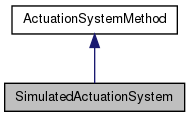
\includegraphics[width=214pt]{class_simulated_actuation_system__inherit__graph}
\end{center}
\end{figure}


\-Collaboration diagram for \-Simulated\-Actuation\-System\-:
\nopagebreak
\begin{figure}[H]
\begin{center}
\leavevmode
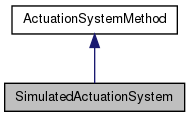
\includegraphics[width=214pt]{class_simulated_actuation_system__coll__graph}
\end{center}
\end{figure}
\subsection*{\-Public \-Types}
\begin{DoxyCompactItemize}
\item 
\hypertarget{class_simulated_actuation_system_a4026d1ead324f05d1c1743024c60d73d}{typedef \*
\-Motion\-Model\-Method\-::\-Motion\-Model\-Pointer {\bfseries \-Motion\-Model\-Pointer}}\label{class_simulated_actuation_system_a4026d1ead324f05d1c1743024c60d73d}

\item 
\hypertarget{class_simulated_actuation_system_a34ed448bdae153ec4719dfc48156be3c}{typedef \*
\-Observation\-Model\-Method\-::\-Observation\-Model\-Pointer {\bfseries \-Observation\-Model\-Pointer}}\label{class_simulated_actuation_system_a34ed448bdae153ec4719dfc48156be3c}

\end{DoxyCompactItemize}
\subsection*{\-Public \-Member \-Functions}
\begin{DoxyCompactItemize}
\item 
\hypertarget{class_simulated_actuation_system_ae6d51c97eff49314b1b4da41ddbf0a77}{{\bfseries \-Simulated\-Actuation\-System} (\-Motion\-Model\-Pointer mm, \-Observation\-Model\-Pointer om)}\label{class_simulated_actuation_system_ae6d51c97eff49314b1b4da41ddbf0a77}

\item 
\hypertarget{class_simulated_actuation_system_a6e5a988011048fcd7df2a68c558f6340}{virtual void {\bfseries apply\-Control} (\-Control\-Type \&u)}\label{class_simulated_actuation_system_a6e5a988011048fcd7df2a68c558f6340}

\item 
\hypertarget{class_simulated_actuation_system_a7a69fe802ad7b1ecbe45e2f221071bee}{virtual \-Observation\-Type {\bfseries get\-Observation} ()}\label{class_simulated_actuation_system_a7a69fe802ad7b1ecbe45e2f221071bee}

\item 
\hypertarget{class_simulated_actuation_system_a7d77f257e56cffbe7133faab50048734}{virtual ompl\-::base\-::\-State $\ast$ {\bfseries get\-True\-State} ()}\label{class_simulated_actuation_system_a7d77f257e56cffbe7133faab50048734}

\item 
\hypertarget{class_simulated_actuation_system_ac6f6e2c9dd429b2d50228b181663ee54}{virtual void {\bfseries set\-True\-State} (const ompl\-::base\-::\-State $\ast$state)}\label{class_simulated_actuation_system_ac6f6e2c9dd429b2d50228b181663ee54}

\item 
\hypertarget{class_simulated_actuation_system_a5d3bdb4d82ffcc98b4bc529ef30f9cfb}{bool {\bfseries check\-Collision} ()}\label{class_simulated_actuation_system_a5d3bdb4d82ffcc98b4bc529ef30f9cfb}

\item 
\hypertarget{class_simulated_actuation_system_a7359da743b5a171e03cff9512c0d6545}{void {\bfseries set\-Belief} (const ompl\-::base\-::\-State $\ast$state)}\label{class_simulated_actuation_system_a7359da743b5a171e03cff9512c0d6545}

\item 
\hypertarget{class_simulated_actuation_system_abe43894eee6e30f630d8f325b30acf12}{virtual \-Motion\-Model\-Pointer {\bfseries get\-Motion\-Model} ()}\label{class_simulated_actuation_system_abe43894eee6e30f630d8f325b30acf12}

\item 
\hypertarget{class_simulated_actuation_system_ad29b96470450e5f2aff883fdffd95e59}{virtual \-Observation\-Model\-Pointer {\bfseries get\-Observation\-Model} ()}\label{class_simulated_actuation_system_ad29b96470450e5f2aff883fdffd95e59}

\end{DoxyCompactItemize}
\subsection*{\-Protected \-Attributes}
\begin{DoxyCompactItemize}
\item 
\hypertarget{class_simulated_actuation_system_a6d2af7c89177a93d2e49a8561c538a1f}{ompl\-::base\-::\-State $\ast$ {\bfseries true\-State\-\_\-}}\label{class_simulated_actuation_system_a6d2af7c89177a93d2e49a8561c538a1f}

\item 
\hypertarget{class_simulated_actuation_system_a28301763f343a04381caae1461a46f7a}{ompl\-::base\-::\-State $\ast$ {\bfseries belief\-\_\-}}\label{class_simulated_actuation_system_a28301763f343a04381caae1461a46f7a}

\end{DoxyCompactItemize}


\-The documentation for this class was generated from the following files\-:\begin{DoxyCompactItemize}
\item 
include/\-Actuation\-Systems/\-Simulated\-Actuation\-System.\-h\item 
src/\-Actuation\-Systems/\-Simulated\-Actuation\-System.\-cpp\end{DoxyCompactItemize}

\hypertarget{classfirm_1_1_space_information}{\section{firm\-:\-:\-Space\-Information \-Class \-Reference}
\label{classfirm_1_1_space_information}\index{firm\-::\-Space\-Information@{firm\-::\-Space\-Information}}
}
\subsection*{\-Public \-Types}
\begin{DoxyCompactItemize}
\item 
\hypertarget{classfirm_1_1_space_information_ad686051bf31885cb46d10e5c9016a6df}{typedef \*
\-Observation\-Model\-Method\-::\-Observation\-Type {\bfseries \-Observation\-Type}}\label{classfirm_1_1_space_information_ad686051bf31885cb46d10e5c9016a6df}

\item 
\hypertarget{classfirm_1_1_space_information_a2caa53f8f7037e2f1b8d70c1077dcf9a}{typedef \*
\-Motion\-Model\-Method\-::\-Motion\-Model\-Pointer {\bfseries \-Motion\-Model\-Pointer}}\label{classfirm_1_1_space_information_a2caa53f8f7037e2f1b8d70c1077dcf9a}

\item 
\hypertarget{classfirm_1_1_space_information_aa31878712d7b14cdaa406dc7b20c8704}{typedef \*
\-Observation\-Model\-Method\-::\-Observation\-Model\-Pointer {\bfseries \-Observation\-Model\-Pointer}}\label{classfirm_1_1_space_information_aa31878712d7b14cdaa406dc7b20c8704}

\item 
\hypertarget{classfirm_1_1_space_information_a6efa9b59d35d1f83427a86271bd47a66}{typedef boost\-::shared\-\_\-ptr\*
$<$ \hyperlink{classfirm_1_1_space_information}{\-Space\-Information} $>$ {\bfseries \-Space\-Information\-Ptr}}\label{classfirm_1_1_space_information_a6efa9b59d35d1f83427a86271bd47a66}

\end{DoxyCompactItemize}
\subsection*{\-Public \-Member \-Functions}
\begin{DoxyCompactItemize}
\item 
\hypertarget{classfirm_1_1_space_information_a18c0788b7b6a56993871f659c6426537}{{\bfseries \-Space\-Information} (const ompl\-::base\-::\-State\-Space\-Ptr \&state\-Space, const ompl\-::control\-::\-Control\-Space\-Ptr \&control\-Space)}\label{classfirm_1_1_space_information_a18c0788b7b6a56993871f659c6426537}

\item 
\hypertarget{classfirm_1_1_space_information_a06dd8787565e1771fbb5060104dc6644}{void {\bfseries set\-Observation\-Model} (\-Observation\-Model\-Pointer om)}\label{classfirm_1_1_space_information_a06dd8787565e1771fbb5060104dc6644}

\item 
\hypertarget{classfirm_1_1_space_information_a90164150ff2eb4e44325dccff69d08a2}{void {\bfseries set\-Motion\-Model} (\-Motion\-Model\-Pointer mm)}\label{classfirm_1_1_space_information_a90164150ff2eb4e44325dccff69d08a2}

\item 
\hypertarget{classfirm_1_1_space_information_a7555e2247318d5b37841816dc3c441b0}{void {\bfseries set\-Belief} (const ompl\-::base\-::\-State $\ast$state)}\label{classfirm_1_1_space_information_a7555e2247318d5b37841816dc3c441b0}

\item 
\hypertarget{classfirm_1_1_space_information_a9aa185374424a90241a1b971fc89aa4a}{void {\bfseries set\-True\-State} (const ompl\-::base\-::\-State $\ast$state)}\label{classfirm_1_1_space_information_a9aa185374424a90241a1b971fc89aa4a}

\item 
\hypertarget{classfirm_1_1_space_information_acdcc00f0bb5d74f66f0d3fb05b44ffb2}{\-Observation\-Model\-Pointer {\bfseries get\-Observation\-Model} (void)}\label{classfirm_1_1_space_information_acdcc00f0bb5d74f66f0d3fb05b44ffb2}

\item 
\hypertarget{classfirm_1_1_space_information_a38dfa45b21cec43a6577e422e19a44ee}{\-Motion\-Model\-Pointer {\bfseries get\-Motion\-Model} (void)}\label{classfirm_1_1_space_information_a38dfa45b21cec43a6577e422e19a44ee}

\item 
\hypertarget{classfirm_1_1_space_information_a99bd9e6ed38a4ace8e0e65063480baa9}{void {\bfseries get\-True\-State} (ompl\-::base\-::\-State $\ast$state)}\label{classfirm_1_1_space_information_a99bd9e6ed38a4ace8e0e65063480baa9}

\item 
\hypertarget{classfirm_1_1_space_information_ac797bd135e3b1ccfa4638a10b413a69d}{bool \hyperlink{classfirm_1_1_space_information_ac797bd135e3b1ccfa4638a10b413a69d}{check\-True\-State\-Validity} (void)}\label{classfirm_1_1_space_information_ac797bd135e3b1ccfa4638a10b413a69d}

\begin{DoxyCompactList}\small\item\em \-Checks whether the true system state is in valid or not. \end{DoxyCompactList}\item 
\hypertarget{classfirm_1_1_space_information_a2cd7942090ff17d9ced900852c4a4955}{void {\bfseries apply\-Control} (const ompl\-::control\-::\-Control $\ast$control)}\label{classfirm_1_1_space_information_a2cd7942090ff17d9ced900852c4a4955}

\item 
\hypertarget{classfirm_1_1_space_information_a3295c828328cbe15dbfdac3c28cd5ccf}{\-Observation\-Type {\bfseries get\-Observation} ()}\label{classfirm_1_1_space_information_a3295c828328cbe15dbfdac3c28cd5ccf}

\end{DoxyCompactItemize}
\subsection*{\-Protected \-Attributes}
\begin{DoxyCompactItemize}
\item 
\hypertarget{classfirm_1_1_space_information_a08dae2888a6ab7e571c89b2a020b175e}{\-Observation\-Model\-Pointer {\bfseries observation\-Model\-\_\-}}\label{classfirm_1_1_space_information_a08dae2888a6ab7e571c89b2a020b175e}

\item 
\hypertarget{classfirm_1_1_space_information_ae911ad91e06bb1eda831c4f7626d0a0e}{\-Motion\-Model\-Pointer {\bfseries motion\-Model\-\_\-}}\label{classfirm_1_1_space_information_ae911ad91e06bb1eda831c4f7626d0a0e}

\item 
\hypertarget{classfirm_1_1_space_information_ada09e25b5d7ff71df94ed2ea85dcb814}{ompl\-::base\-::\-State $\ast$ {\bfseries true\-State\-\_\-}}\label{classfirm_1_1_space_information_ada09e25b5d7ff71df94ed2ea85dcb814}

\item 
\hypertarget{classfirm_1_1_space_information_a14f18dfbbb3a3a6329309752fb5d2f23}{ompl\-::base\-::\-State $\ast$ {\bfseries belief\-\_\-}}\label{classfirm_1_1_space_information_a14f18dfbbb3a3a6329309752fb5d2f23}

\end{DoxyCompactItemize}


\-The documentation for this class was generated from the following files\-:\begin{DoxyCompactItemize}
\item 
include/\-Space\-Information/\-Space\-Information.\-h\item 
src/\-Space\-Information/\-Space\-Information.\-cpp\end{DoxyCompactItemize}

\hypertarget{class_s_e2_belief_space_1_1_state_type}{\section{\-S\-E2\-Belief\-Space\-:\-:\-State\-Type \-Class \-Reference}
\label{class_s_e2_belief_space_1_1_state_type}\index{\-S\-E2\-Belief\-Space\-::\-State\-Type@{\-S\-E2\-Belief\-Space\-::\-State\-Type}}
}


\-A belief in \-S\-E(2)\-: (x, y, yaw, covariance)  




{\ttfamily \#include $<$\-S\-E2\-Belief\-Space.\-h$>$}

\subsection*{\-Public \-Member \-Functions}
\begin{DoxyCompactItemize}
\item 
\hypertarget{class_s_e2_belief_space_1_1_state_type_a387c4a054850471f2e6eb53b354a5b06}{double \hyperlink{class_s_e2_belief_space_1_1_state_type_a387c4a054850471f2e6eb53b354a5b06}{get\-X} (void) const }\label{class_s_e2_belief_space_1_1_state_type_a387c4a054850471f2e6eb53b354a5b06}

\begin{DoxyCompactList}\small\item\em \-Get the \-X component of the state. \end{DoxyCompactList}\item 
\hypertarget{class_s_e2_belief_space_1_1_state_type_a8e32b9c1c8da1bb687d33801d5805fdd}{double \hyperlink{class_s_e2_belief_space_1_1_state_type_a8e32b9c1c8da1bb687d33801d5805fdd}{get\-Y} (void) const }\label{class_s_e2_belief_space_1_1_state_type_a8e32b9c1c8da1bb687d33801d5805fdd}

\begin{DoxyCompactList}\small\item\em \-Get the \-Y component of the state. \end{DoxyCompactList}\item 
\hypertarget{class_s_e2_belief_space_1_1_state_type_a1ae660667f7db3285e341570f3ee2da0}{double \hyperlink{class_s_e2_belief_space_1_1_state_type_a1ae660667f7db3285e341570f3ee2da0}{get\-Yaw} (void) const }\label{class_s_e2_belief_space_1_1_state_type_a1ae660667f7db3285e341570f3ee2da0}

\begin{DoxyCompactList}\small\item\em \-Get the yaw component of the state. \-This is the rotation in plane, with respect to the \-Z axis. \end{DoxyCompactList}\item 
\hypertarget{class_s_e2_belief_space_1_1_state_type_a604a4895fd3b2bdcbfb815e8d49b399c}{arma\-::mat {\bfseries get\-Covariance} (void) const }\label{class_s_e2_belief_space_1_1_state_type_a604a4895fd3b2bdcbfb815e8d49b399c}

\item 
\hypertarget{class_s_e2_belief_space_1_1_state_type_aafa60b4810c40a106fb5db62fde17026}{void \hyperlink{class_s_e2_belief_space_1_1_state_type_aafa60b4810c40a106fb5db62fde17026}{set\-X} (double x)}\label{class_s_e2_belief_space_1_1_state_type_aafa60b4810c40a106fb5db62fde17026}

\begin{DoxyCompactList}\small\item\em \-Set the \-X component of the state. \end{DoxyCompactList}\item 
\hypertarget{class_s_e2_belief_space_1_1_state_type_a26d653e2790a61a3ba36158e3afeb930}{void \hyperlink{class_s_e2_belief_space_1_1_state_type_a26d653e2790a61a3ba36158e3afeb930}{set\-Y} (double y)}\label{class_s_e2_belief_space_1_1_state_type_a26d653e2790a61a3ba36158e3afeb930}

\begin{DoxyCompactList}\small\item\em \-Set the \-Y component of the state. \end{DoxyCompactList}\item 
\hypertarget{class_s_e2_belief_space_1_1_state_type_aba839217241393594cacff450a61cc56}{void \hyperlink{class_s_e2_belief_space_1_1_state_type_aba839217241393594cacff450a61cc56}{set\-X\-Y} (double x, double y)}\label{class_s_e2_belief_space_1_1_state_type_aba839217241393594cacff450a61cc56}

\begin{DoxyCompactList}\small\item\em \-Set the \-X and \-Y components of the state. \end{DoxyCompactList}\item 
\hypertarget{class_s_e2_belief_space_1_1_state_type_a86f79402419f759c39ee3d6bfd7b375f}{void \hyperlink{class_s_e2_belief_space_1_1_state_type_a86f79402419f759c39ee3d6bfd7b375f}{set\-Yaw} (double yaw)}\label{class_s_e2_belief_space_1_1_state_type_a86f79402419f759c39ee3d6bfd7b375f}

\begin{DoxyCompactList}\small\item\em \-Set the yaw component of the state. \-This is the rotation in plane, with respect to the \-Z axis. \end{DoxyCompactList}\item 
\hypertarget{class_s_e2_belief_space_1_1_state_type_af6e888798cdd76ae3ae56c23e6d14bca}{void {\bfseries set\-X\-Y\-Yaw} (double x, double y, double yaw)}\label{class_s_e2_belief_space_1_1_state_type_af6e888798cdd76ae3ae56c23e6d14bca}

\item 
\hypertarget{class_s_e2_belief_space_1_1_state_type_a5fee8a9eb77fd9ee5b7a7e889adf0602}{void {\bfseries set\-Covariance} (arma\-::mat cov)}\label{class_s_e2_belief_space_1_1_state_type_a5fee8a9eb77fd9ee5b7a7e889adf0602}

\item 
\hypertarget{class_s_e2_belief_space_1_1_state_type_a7514b225050bf07ab431a25371af3f1c}{arma\-::colvec {\bfseries get\-Arma\-Data} (void) const }\label{class_s_e2_belief_space_1_1_state_type_a7514b225050bf07ab431a25371af3f1c}

\end{DoxyCompactItemize}
\subsection*{\-Static \-Public \-Attributes}
\begin{DoxyCompactItemize}
\item 
\hypertarget{class_s_e2_belief_space_1_1_state_type_a4f0f638f62e339fd8cdcb43b3c49f2a6}{static double {\bfseries mean\-Norm\-Weight\-\_\-}}\label{class_s_e2_belief_space_1_1_state_type_a4f0f638f62e339fd8cdcb43b3c49f2a6}

\item 
\hypertarget{class_s_e2_belief_space_1_1_state_type_accb04f4d8d86cd9ba3626f2a96611fff}{static double {\bfseries cov\-Norm\-Weight\-\_\-}}\label{class_s_e2_belief_space_1_1_state_type_accb04f4d8d86cd9ba3626f2a96611fff}

\end{DoxyCompactItemize}


\subsection{\-Detailed \-Description}
\-A belief in \-S\-E(2)\-: (x, y, yaw, covariance) 

\-The documentation for this class was generated from the following file\-:\begin{DoxyCompactItemize}
\item 
include/\-Spaces/\-S\-E2\-Belief\-Space.\-h\end{DoxyCompactItemize}

\hypertarget{class_ti_xml_attribute}{\section{\-Ti\-Xml\-Attribute \-Class \-Reference}
\label{class_ti_xml_attribute}\index{\-Ti\-Xml\-Attribute@{\-Ti\-Xml\-Attribute}}
}


{\ttfamily \#include $<$tinyxml.\-h$>$}



\-Inheritance diagram for \-Ti\-Xml\-Attribute\-:\nopagebreak
\begin{figure}[H]
\begin{center}
\leavevmode
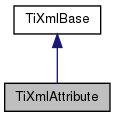
\includegraphics[width=158pt]{class_ti_xml_attribute__inherit__graph}
\end{center}
\end{figure}


\-Collaboration diagram for \-Ti\-Xml\-Attribute\-:\nopagebreak
\begin{figure}[H]
\begin{center}
\leavevmode
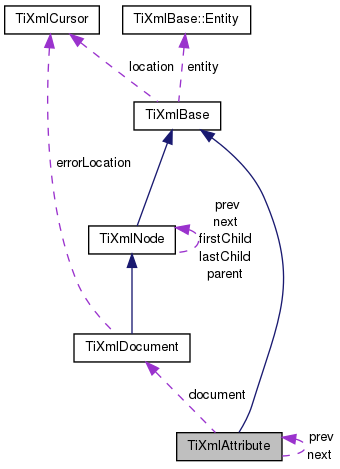
\includegraphics[width=327pt]{class_ti_xml_attribute__coll__graph}
\end{center}
\end{figure}
\subsection*{\-Public \-Member \-Functions}
\begin{DoxyCompactItemize}
\item 
\hypertarget{class_ti_xml_attribute_a9cfa3c8179873fd485d83003b114f8e1}{\hyperlink{class_ti_xml_attribute_a9cfa3c8179873fd485d83003b114f8e1}{\-Ti\-Xml\-Attribute} ()}\label{class_ti_xml_attribute_a9cfa3c8179873fd485d83003b114f8e1}

\begin{DoxyCompactList}\small\item\em \-Construct an empty attribute. \end{DoxyCompactList}\item 
\hypertarget{class_ti_xml_attribute_a759d0b76fb8fcf765ecab243bc14f05e}{\hyperlink{class_ti_xml_attribute_a759d0b76fb8fcf765ecab243bc14f05e}{\-Ti\-Xml\-Attribute} (const char $\ast$\-\_\-name, const char $\ast$\-\_\-value)}\label{class_ti_xml_attribute_a759d0b76fb8fcf765ecab243bc14f05e}

\begin{DoxyCompactList}\small\item\em \-Construct an attribute with a name and value. \end{DoxyCompactList}\item 
\hypertarget{class_ti_xml_attribute_a298a57287d305904ba6bd96ae6f78d3d}{const char $\ast$ \hyperlink{class_ti_xml_attribute_a298a57287d305904ba6bd96ae6f78d3d}{\-Name} () const }\label{class_ti_xml_attribute_a298a57287d305904ba6bd96ae6f78d3d}

\begin{DoxyCompactList}\small\item\em \-Return the name of this attribute. \end{DoxyCompactList}\item 
\hypertarget{class_ti_xml_attribute_a0f874490eac8ca00ee0070765d0e97e3}{const char $\ast$ \hyperlink{class_ti_xml_attribute_a0f874490eac8ca00ee0070765d0e97e3}{\-Value} () const }\label{class_ti_xml_attribute_a0f874490eac8ca00ee0070765d0e97e3}

\begin{DoxyCompactList}\small\item\em \-Return the value of this attribute. \end{DoxyCompactList}\item 
\hypertarget{class_ti_xml_attribute_aa1a20ad59dc7e89a0ab265396360d50f}{int \hyperlink{class_ti_xml_attribute_aa1a20ad59dc7e89a0ab265396360d50f}{\-Int\-Value} () const }\label{class_ti_xml_attribute_aa1a20ad59dc7e89a0ab265396360d50f}

\begin{DoxyCompactList}\small\item\em \-Return the value of this attribute, converted to an integer. \end{DoxyCompactList}\item 
\hypertarget{class_ti_xml_attribute_a2880ddef53fc7522c99535273954d230}{double \hyperlink{class_ti_xml_attribute_a2880ddef53fc7522c99535273954d230}{\-Double\-Value} () const }\label{class_ti_xml_attribute_a2880ddef53fc7522c99535273954d230}

\begin{DoxyCompactList}\small\item\em \-Return the value of this attribute, converted to a double. \end{DoxyCompactList}\item 
\hypertarget{class_ti_xml_attribute_a64cee17bceb8232eb0736d26dd082d79}{const \-T\-I\-X\-M\-L\-\_\-\-S\-T\-R\-I\-N\-G \& {\bfseries \-Name\-T\-Str} () const }\label{class_ti_xml_attribute_a64cee17bceb8232eb0736d26dd082d79}

\item 
int \hyperlink{class_ti_xml_attribute_ad6c93088ee21af41a107931223339344}{\-Query\-Int\-Value} (int $\ast$\-\_\-value) const 
\item 
\hypertarget{class_ti_xml_attribute_ac87b2a8489906a5d7aa2875f20be3513}{int \hyperlink{class_ti_xml_attribute_ac87b2a8489906a5d7aa2875f20be3513}{\-Query\-Double\-Value} (double $\ast$\-\_\-value) const }\label{class_ti_xml_attribute_ac87b2a8489906a5d7aa2875f20be3513}

\begin{DoxyCompactList}\small\item\em \-Query\-Double\-Value examines the value string. \-See \hyperlink{class_ti_xml_attribute_ad6c93088ee21af41a107931223339344}{\-Query\-Int\-Value()}. \end{DoxyCompactList}\item 
\hypertarget{class_ti_xml_attribute_ab7fa3d21ff8d7c5764cf9af15b667a99}{void \hyperlink{class_ti_xml_attribute_ab7fa3d21ff8d7c5764cf9af15b667a99}{\-Set\-Name} (const char $\ast$\-\_\-name)}\label{class_ti_xml_attribute_ab7fa3d21ff8d7c5764cf9af15b667a99}

\begin{DoxyCompactList}\small\item\em \-Set the name of this attribute. \end{DoxyCompactList}\item 
\hypertarget{class_ti_xml_attribute_a2dae44178f668b3cb48101be4f2236a0}{void \hyperlink{class_ti_xml_attribute_a2dae44178f668b3cb48101be4f2236a0}{\-Set\-Value} (const char $\ast$\-\_\-value)}\label{class_ti_xml_attribute_a2dae44178f668b3cb48101be4f2236a0}

\begin{DoxyCompactList}\small\item\em \-Set the value. \end{DoxyCompactList}\item 
\hypertarget{class_ti_xml_attribute_a7e065df640116a62ea4f4b7da5449cc8}{void \hyperlink{class_ti_xml_attribute_a7e065df640116a62ea4f4b7da5449cc8}{\-Set\-Int\-Value} (int \-\_\-value)}\label{class_ti_xml_attribute_a7e065df640116a62ea4f4b7da5449cc8}

\begin{DoxyCompactList}\small\item\em \-Set the value from an integer. \end{DoxyCompactList}\item 
\hypertarget{class_ti_xml_attribute_a0316da31373496c4368ad549bf711394}{void \hyperlink{class_ti_xml_attribute_a0316da31373496c4368ad549bf711394}{\-Set\-Double\-Value} (double \-\_\-value)}\label{class_ti_xml_attribute_a0316da31373496c4368ad549bf711394}

\begin{DoxyCompactList}\small\item\em \-Set the value from a double. \end{DoxyCompactList}\item 
\hypertarget{class_ti_xml_attribute_a776478980776a024f7c2846eec640f65}{const \hyperlink{class_ti_xml_attribute}{\-Ti\-Xml\-Attribute} $\ast$ \hyperlink{class_ti_xml_attribute_a776478980776a024f7c2846eec640f65}{\-Next} () const }\label{class_ti_xml_attribute_a776478980776a024f7c2846eec640f65}

\begin{DoxyCompactList}\small\item\em \-Get the next sibling attribute in the \-D\-O\-M. \-Returns null at end. \end{DoxyCompactList}\item 
\hypertarget{class_ti_xml_attribute_a138320aa7793b148ba7e5bd0a0ea4db6}{\hyperlink{class_ti_xml_attribute}{\-Ti\-Xml\-Attribute} $\ast$ {\bfseries \-Next} ()}\label{class_ti_xml_attribute_a138320aa7793b148ba7e5bd0a0ea4db6}

\item 
\hypertarget{class_ti_xml_attribute_a54a5f8730c7b02b9a41b74e12e27fe86}{const \hyperlink{class_ti_xml_attribute}{\-Ti\-Xml\-Attribute} $\ast$ \hyperlink{class_ti_xml_attribute_a54a5f8730c7b02b9a41b74e12e27fe86}{\-Previous} () const }\label{class_ti_xml_attribute_a54a5f8730c7b02b9a41b74e12e27fe86}

\begin{DoxyCompactList}\small\item\em \-Get the previous sibling attribute in the \-D\-O\-M. \-Returns null at beginning. \end{DoxyCompactList}\item 
\hypertarget{class_ti_xml_attribute_ae4dabc932cba945ed1e92fec5f121193}{\hyperlink{class_ti_xml_attribute}{\-Ti\-Xml\-Attribute} $\ast$ {\bfseries \-Previous} ()}\label{class_ti_xml_attribute_ae4dabc932cba945ed1e92fec5f121193}

\item 
\hypertarget{class_ti_xml_attribute_ae48c2a65b520d453914ce4e845d607cf}{bool {\bfseries operator==} (const \hyperlink{class_ti_xml_attribute}{\-Ti\-Xml\-Attribute} \&rhs) const }\label{class_ti_xml_attribute_ae48c2a65b520d453914ce4e845d607cf}

\item 
\hypertarget{class_ti_xml_attribute_adb8b6f2cad5948e73e383182e7ce10de}{bool {\bfseries operator$<$} (const \hyperlink{class_ti_xml_attribute}{\-Ti\-Xml\-Attribute} \&rhs) const }\label{class_ti_xml_attribute_adb8b6f2cad5948e73e383182e7ce10de}

\item 
\hypertarget{class_ti_xml_attribute_a867562769ef9778c1690cd373246b05b}{bool {\bfseries operator$>$} (const \hyperlink{class_ti_xml_attribute}{\-Ti\-Xml\-Attribute} \&rhs) const }\label{class_ti_xml_attribute_a867562769ef9778c1690cd373246b05b}

\item 
\hypertarget{class_ti_xml_attribute_ad62774421b814894b995af3b5d231dda}{virtual const char $\ast$ {\bfseries \-Parse} (const char $\ast$p, \hyperlink{class_ti_xml_parsing_data}{\-Ti\-Xml\-Parsing\-Data} $\ast$data, \-Ti\-Xml\-Encoding encoding)}\label{class_ti_xml_attribute_ad62774421b814894b995af3b5d231dda}

\item 
virtual void \hyperlink{class_ti_xml_attribute_acc04956c1d5c4c31fe74f7a7528d109a}{\-Print} (\-F\-I\-L\-E $\ast$cfile, int depth) const 
\item 
\hypertarget{class_ti_xml_attribute_a19e6b6862a80b188571c47947e88d030}{void {\bfseries \-Print} (\-F\-I\-L\-E $\ast$cfile, int depth, \-T\-I\-X\-M\-L\-\_\-\-S\-T\-R\-I\-N\-G $\ast$str) const }\label{class_ti_xml_attribute_a19e6b6862a80b188571c47947e88d030}

\item 
\hypertarget{class_ti_xml_attribute_ac12a94d4548302afb12f488ba101f7d1}{void {\bfseries \-Set\-Document} (\hyperlink{class_ti_xml_document}{\-Ti\-Xml\-Document} $\ast$doc)}\label{class_ti_xml_attribute_ac12a94d4548302afb12f488ba101f7d1}

\end{DoxyCompactItemize}
\subsection*{\-Private \-Member \-Functions}
\begin{DoxyCompactItemize}
\item 
\hypertarget{class_ti_xml_attribute_aee53e434ace7271afc5ce51aeea0b400}{{\bfseries \-Ti\-Xml\-Attribute} (const \hyperlink{class_ti_xml_attribute}{\-Ti\-Xml\-Attribute} \&)}\label{class_ti_xml_attribute_aee53e434ace7271afc5ce51aeea0b400}

\item 
\hypertarget{class_ti_xml_attribute_a83b9c2a47dbfadf5029f2c0f13c18466}{void {\bfseries operator=} (const \hyperlink{class_ti_xml_attribute}{\-Ti\-Xml\-Attribute} \&base)}\label{class_ti_xml_attribute_a83b9c2a47dbfadf5029f2c0f13c18466}

\end{DoxyCompactItemize}
\subsection*{\-Private \-Attributes}
\begin{DoxyCompactItemize}
\item 
\hypertarget{class_ti_xml_attribute_ada41d3cff50cd33a78072806f88d4433}{\hyperlink{class_ti_xml_document}{\-Ti\-Xml\-Document} $\ast$ {\bfseries document}}\label{class_ti_xml_attribute_ada41d3cff50cd33a78072806f88d4433}

\item 
\hypertarget{class_ti_xml_attribute_afcbe165f33f08cf9b24daa33f0ee951a}{\-T\-I\-X\-M\-L\-\_\-\-S\-T\-R\-I\-N\-G {\bfseries name}}\label{class_ti_xml_attribute_afcbe165f33f08cf9b24daa33f0ee951a}

\item 
\hypertarget{class_ti_xml_attribute_ae9e4e5f442347434b1da43954cc1b411}{\-T\-I\-X\-M\-L\-\_\-\-S\-T\-R\-I\-N\-G {\bfseries value}}\label{class_ti_xml_attribute_ae9e4e5f442347434b1da43954cc1b411}

\item 
\hypertarget{class_ti_xml_attribute_aaf6c6272c625fbf38e571cbf570ea94a}{\hyperlink{class_ti_xml_attribute}{\-Ti\-Xml\-Attribute} $\ast$ {\bfseries prev}}\label{class_ti_xml_attribute_aaf6c6272c625fbf38e571cbf570ea94a}

\item 
\hypertarget{class_ti_xml_attribute_ae851adf61b80cf45b797fee77dea135f}{\hyperlink{class_ti_xml_attribute}{\-Ti\-Xml\-Attribute} $\ast$ {\bfseries next}}\label{class_ti_xml_attribute_ae851adf61b80cf45b797fee77dea135f}

\end{DoxyCompactItemize}
\subsection*{\-Friends}
\begin{DoxyCompactItemize}
\item 
\hypertarget{class_ti_xml_attribute_a35a7b7f89f708527677d5078d41ce0bf}{class {\bfseries \-Ti\-Xml\-Attribute\-Set}}\label{class_ti_xml_attribute_a35a7b7f89f708527677d5078d41ce0bf}

\end{DoxyCompactItemize}


\subsection{\-Detailed \-Description}
\-An attribute is a name-\/value pair. \-Elements have an arbitrary number of attributes, each with a unique name.

\begin{DoxyNote}{\-Note}
\-The attributes are not \-Ti\-Xml\-Nodes, since they are not part of the tiny\-X\-M\-L document object model. \-There are other suggested ways to look at this problem. 
\end{DoxyNote}


\subsection{\-Member \-Function \-Documentation}
\hypertarget{class_ti_xml_attribute_acc04956c1d5c4c31fe74f7a7528d109a}{\index{\-Ti\-Xml\-Attribute@{\-Ti\-Xml\-Attribute}!\-Print@{\-Print}}
\index{\-Print@{\-Print}!TiXmlAttribute@{\-Ti\-Xml\-Attribute}}
\subsubsection[{\-Print}]{\setlength{\rightskip}{0pt plus 5cm}virtual void {\bf \-Ti\-Xml\-Attribute\-::\-Print} (
\begin{DoxyParamCaption}
\item[{\-F\-I\-L\-E $\ast$}]{cfile, }
\item[{int}]{depth}
\end{DoxyParamCaption}
) const\hspace{0.3cm}{\ttfamily  \mbox{[}inline, virtual\mbox{]}}}}\label{class_ti_xml_attribute_acc04956c1d5c4c31fe74f7a7528d109a}
\-All \-Tiny\-Xml classes can print themselves to a filestream or the string class (\hyperlink{class_ti_xml_string}{\-Ti\-Xml\-String} in non-\/\-S\-T\-L mode, std\-::string in \-S\-T\-L mode.) \-Either or both cfile and str can be null.

\-This is a formatted print, and will insert tabs and newlines.

(\-For an unformatted stream, use the $<$$<$ operator.) 

\-Implements \hyperlink{class_ti_xml_base_a0de56b3f2ef14c65091a3b916437b512}{\-Ti\-Xml\-Base}.

\hypertarget{class_ti_xml_attribute_ad6c93088ee21af41a107931223339344}{\index{\-Ti\-Xml\-Attribute@{\-Ti\-Xml\-Attribute}!\-Query\-Int\-Value@{\-Query\-Int\-Value}}
\index{\-Query\-Int\-Value@{\-Query\-Int\-Value}!TiXmlAttribute@{\-Ti\-Xml\-Attribute}}
\subsubsection[{\-Query\-Int\-Value}]{\setlength{\rightskip}{0pt plus 5cm}int {\bf \-Ti\-Xml\-Attribute\-::\-Query\-Int\-Value} (
\begin{DoxyParamCaption}
\item[{int $\ast$}]{\-\_\-value}
\end{DoxyParamCaption}
) const}}\label{class_ti_xml_attribute_ad6c93088ee21af41a107931223339344}
\-Query\-Int\-Value examines the value string. \-It is an alternative to the \hyperlink{class_ti_xml_attribute_aa1a20ad59dc7e89a0ab265396360d50f}{\-Int\-Value()} method with richer error checking. \-If the value is an integer, it is stored in 'value' and the call returns \-T\-I\-X\-M\-L\-\_\-\-S\-U\-C\-C\-E\-S\-S. \-If it is not an integer, it returns \-T\-I\-X\-M\-L\-\_\-\-W\-R\-O\-N\-G\-\_\-\-T\-Y\-P\-E.

\-A specialized but useful call. \-Note that for success it returns 0, which is the opposite of almost all other \-Tiny\-Xml calls. 

\-The documentation for this class was generated from the following files\-:\begin{DoxyCompactItemize}
\item 
tinyxml/tinyxml.\-h\item 
tinyxml/tinyxml.\-cpp\item 
tinyxml/tinyxmlparser.\-cpp\end{DoxyCompactItemize}

\hypertarget{class_ti_xml_attribute_set}{\section{\-Ti\-Xml\-Attribute\-Set \-Class \-Reference}
\label{class_ti_xml_attribute_set}\index{\-Ti\-Xml\-Attribute\-Set@{\-Ti\-Xml\-Attribute\-Set}}
}
\subsection*{\-Public \-Member \-Functions}
\begin{DoxyCompactItemize}
\item 
\hypertarget{class_ti_xml_attribute_set_a745e50ddaae3bee93e4589321e0b9c1a}{void {\bfseries \-Add} (\hyperlink{class_ti_xml_attribute}{\-Ti\-Xml\-Attribute} $\ast$attribute)}\label{class_ti_xml_attribute_set_a745e50ddaae3bee93e4589321e0b9c1a}

\item 
\hypertarget{class_ti_xml_attribute_set_a924a73d071f2573f9060f0be57879c57}{void {\bfseries \-Remove} (\hyperlink{class_ti_xml_attribute}{\-Ti\-Xml\-Attribute} $\ast$attribute)}\label{class_ti_xml_attribute_set_a924a73d071f2573f9060f0be57879c57}

\item 
\hypertarget{class_ti_xml_attribute_set_ae0636e88cedd4b09d61c451860f68598}{const \hyperlink{class_ti_xml_attribute}{\-Ti\-Xml\-Attribute} $\ast$ {\bfseries \-First} () const }\label{class_ti_xml_attribute_set_ae0636e88cedd4b09d61c451860f68598}

\item 
\hypertarget{class_ti_xml_attribute_set_a99703bb08ca2aece2d7ef835de339ba0}{\hyperlink{class_ti_xml_attribute}{\-Ti\-Xml\-Attribute} $\ast$ {\bfseries \-First} ()}\label{class_ti_xml_attribute_set_a99703bb08ca2aece2d7ef835de339ba0}

\item 
\hypertarget{class_ti_xml_attribute_set_a7b3f3ccf39a97bc25539d3fcc540296a}{const \hyperlink{class_ti_xml_attribute}{\-Ti\-Xml\-Attribute} $\ast$ {\bfseries \-Last} () const }\label{class_ti_xml_attribute_set_a7b3f3ccf39a97bc25539d3fcc540296a}

\item 
\hypertarget{class_ti_xml_attribute_set_ab4c4edfb2d74f6ea31aae096743bd6e0}{\hyperlink{class_ti_xml_attribute}{\-Ti\-Xml\-Attribute} $\ast$ {\bfseries \-Last} ()}\label{class_ti_xml_attribute_set_ab4c4edfb2d74f6ea31aae096743bd6e0}

\item 
\hypertarget{class_ti_xml_attribute_set_af3675cc2bfd0aea153cda1cfcdd1f77e}{\hyperlink{class_ti_xml_attribute}{\-Ti\-Xml\-Attribute} $\ast$ {\bfseries \-Find} (const char $\ast$\-\_\-name) const }\label{class_ti_xml_attribute_set_af3675cc2bfd0aea153cda1cfcdd1f77e}

\item 
\hypertarget{class_ti_xml_attribute_set_a5e28f5d32f048fba85d04dc317495bdc}{\hyperlink{class_ti_xml_attribute}{\-Ti\-Xml\-Attribute} $\ast$ {\bfseries \-Find\-Or\-Create} (const char $\ast$\-\_\-name)}\label{class_ti_xml_attribute_set_a5e28f5d32f048fba85d04dc317495bdc}

\end{DoxyCompactItemize}


\-The documentation for this class was generated from the following files\-:\begin{DoxyCompactItemize}
\item 
tinyxml/tinyxml.\-h\item 
tinyxml/tinyxml.\-cpp\end{DoxyCompactItemize}

\hypertarget{class_ti_xml_base}{\section{\-Ti\-Xml\-Base \-Class \-Reference}
\label{class_ti_xml_base}\index{\-Ti\-Xml\-Base@{\-Ti\-Xml\-Base}}
}


{\ttfamily \#include $<$tinyxml.\-h$>$}



\-Inheritance diagram for \-Ti\-Xml\-Base\-:\nopagebreak
\begin{figure}[H]
\begin{center}
\leavevmode
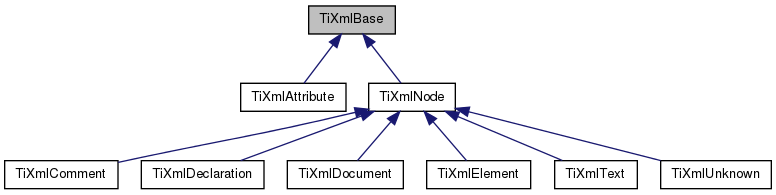
\includegraphics[width=350pt]{class_ti_xml_base__inherit__graph}
\end{center}
\end{figure}


\-Collaboration diagram for \-Ti\-Xml\-Base\-:
\nopagebreak
\begin{figure}[H]
\begin{center}
\leavevmode
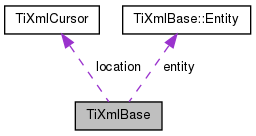
\includegraphics[width=264pt]{class_ti_xml_base__coll__graph}
\end{center}
\end{figure}
\subsection*{\-Classes}
\begin{DoxyCompactItemize}
\item 
struct \hyperlink{struct_ti_xml_base_1_1_entity}{\-Entity}
\end{DoxyCompactItemize}
\subsection*{\-Public \-Types}
\begin{DoxyCompactItemize}
\item 
enum \{ \*
{\bfseries \-T\-I\-X\-M\-L\-\_\-\-N\-O\-\_\-\-E\-R\-R\-O\-R} =  0, 
{\bfseries \-T\-I\-X\-M\-L\-\_\-\-E\-R\-R\-O\-R}, 
{\bfseries \-T\-I\-X\-M\-L\-\_\-\-E\-R\-R\-O\-R\-\_\-\-O\-P\-E\-N\-I\-N\-G\-\_\-\-F\-I\-L\-E}, 
{\bfseries \-T\-I\-X\-M\-L\-\_\-\-E\-R\-R\-O\-R\-\_\-\-P\-A\-R\-S\-I\-N\-G\-\_\-\-E\-L\-E\-M\-E\-N\-T}, 
\*
{\bfseries \-T\-I\-X\-M\-L\-\_\-\-E\-R\-R\-O\-R\-\_\-\-F\-A\-I\-L\-E\-D\-\_\-\-T\-O\-\_\-\-R\-E\-A\-D\-\_\-\-E\-L\-E\-M\-E\-N\-T\-\_\-\-N\-A\-M\-E}, 
{\bfseries \-T\-I\-X\-M\-L\-\_\-\-E\-R\-R\-O\-R\-\_\-\-R\-E\-A\-D\-I\-N\-G\-\_\-\-E\-L\-E\-M\-E\-N\-T\-\_\-\-V\-A\-L\-U\-E}, 
{\bfseries \-T\-I\-X\-M\-L\-\_\-\-E\-R\-R\-O\-R\-\_\-\-R\-E\-A\-D\-I\-N\-G\-\_\-\-A\-T\-T\-R\-I\-B\-U\-T\-E\-S}, 
{\bfseries \-T\-I\-X\-M\-L\-\_\-\-E\-R\-R\-O\-R\-\_\-\-P\-A\-R\-S\-I\-N\-G\-\_\-\-E\-M\-P\-T\-Y}, 
\*
{\bfseries \-T\-I\-X\-M\-L\-\_\-\-E\-R\-R\-O\-R\-\_\-\-R\-E\-A\-D\-I\-N\-G\-\_\-\-E\-N\-D\-\_\-\-T\-A\-G}, 
{\bfseries \-T\-I\-X\-M\-L\-\_\-\-E\-R\-R\-O\-R\-\_\-\-P\-A\-R\-S\-I\-N\-G\-\_\-\-U\-N\-K\-N\-O\-W\-N}, 
{\bfseries \-T\-I\-X\-M\-L\-\_\-\-E\-R\-R\-O\-R\-\_\-\-P\-A\-R\-S\-I\-N\-G\-\_\-\-C\-O\-M\-M\-E\-N\-T}, 
{\bfseries \-T\-I\-X\-M\-L\-\_\-\-E\-R\-R\-O\-R\-\_\-\-P\-A\-R\-S\-I\-N\-G\-\_\-\-D\-E\-C\-L\-A\-R\-A\-T\-I\-O\-N}, 
\*
{\bfseries \-T\-I\-X\-M\-L\-\_\-\-E\-R\-R\-O\-R\-\_\-\-D\-O\-C\-U\-M\-E\-N\-T\-\_\-\-E\-M\-P\-T\-Y}, 
{\bfseries \-T\-I\-X\-M\-L\-\_\-\-E\-R\-R\-O\-R\-\_\-\-E\-M\-B\-E\-D\-D\-E\-D\-\_\-\-N\-U\-L\-L}, 
{\bfseries \-T\-I\-X\-M\-L\-\_\-\-E\-R\-R\-O\-R\-\_\-\-P\-A\-R\-S\-I\-N\-G\-\_\-\-C\-D\-A\-T\-A}, 
{\bfseries \-T\-I\-X\-M\-L\-\_\-\-E\-R\-R\-O\-R\-\_\-\-D\-O\-C\-U\-M\-E\-N\-T\-\_\-\-T\-O\-P\-\_\-\-O\-N\-L\-Y}, 
\*
{\bfseries \-T\-I\-X\-M\-L\-\_\-\-E\-R\-R\-O\-R\-\_\-\-S\-T\-R\-I\-N\-G\-\_\-\-C\-O\-U\-N\-T}
 \}
\end{DoxyCompactItemize}
\subsection*{\-Public \-Member \-Functions}
\begin{DoxyCompactItemize}
\item 
virtual void \hyperlink{class_ti_xml_base_a0de56b3f2ef14c65091a3b916437b512}{\-Print} (\-F\-I\-L\-E $\ast$cfile, int depth) const =0
\item 
int \hyperlink{class_ti_xml_base_a024bceb070188df92c2a8d8852dd0853}{\-Row} () const 
\item 
\hypertarget{class_ti_xml_base_ab54bfb9b70fe6dd276e7b279cab7f003}{int \hyperlink{class_ti_xml_base_ab54bfb9b70fe6dd276e7b279cab7f003}{\-Column} () const }\label{class_ti_xml_base_ab54bfb9b70fe6dd276e7b279cab7f003}

\begin{DoxyCompactList}\small\item\em \-See \hyperlink{class_ti_xml_base_a024bceb070188df92c2a8d8852dd0853}{\-Row()} \end{DoxyCompactList}\item 
\hypertarget{class_ti_xml_base_ac6b3e0f790930d4970ec30764e937b5d}{void \hyperlink{class_ti_xml_base_ac6b3e0f790930d4970ec30764e937b5d}{\-Set\-User\-Data} (void $\ast$user)}\label{class_ti_xml_base_ac6b3e0f790930d4970ec30764e937b5d}

\begin{DoxyCompactList}\small\item\em \-Set a pointer to arbitrary user data. \end{DoxyCompactList}\item 
\hypertarget{class_ti_xml_base_a6559a530ca6763fc301a14d77ed28c17}{void $\ast$ \hyperlink{class_ti_xml_base_a6559a530ca6763fc301a14d77ed28c17}{\-Get\-User\-Data} ()}\label{class_ti_xml_base_a6559a530ca6763fc301a14d77ed28c17}

\begin{DoxyCompactList}\small\item\em \-Get a pointer to arbitrary user data. \end{DoxyCompactList}\item 
\hypertarget{class_ti_xml_base_ad0120210e4680ef2088601753ce0ede4}{const void $\ast$ \hyperlink{class_ti_xml_base_ad0120210e4680ef2088601753ce0ede4}{\-Get\-User\-Data} () const }\label{class_ti_xml_base_ad0120210e4680ef2088601753ce0ede4}

\begin{DoxyCompactList}\small\item\em \-Get a pointer to arbitrary user data. \end{DoxyCompactList}\item 
\hypertarget{class_ti_xml_base_a00e4edb0219d00a1379c856e5a1d2025}{virtual const char $\ast$ {\bfseries \-Parse} (const char $\ast$p, \hyperlink{class_ti_xml_parsing_data}{\-Ti\-Xml\-Parsing\-Data} $\ast$data, \-Ti\-Xml\-Encoding encoding)=0}\label{class_ti_xml_base_a00e4edb0219d00a1379c856e5a1d2025}

\end{DoxyCompactItemize}
\subsection*{\-Static \-Public \-Member \-Functions}
\begin{DoxyCompactItemize}
\item 
static void \hyperlink{class_ti_xml_base_a0f799ec645bfb8d8a969e83478f379c1}{\-Set\-Condense\-White\-Space} (bool condense)
\item 
\hypertarget{class_ti_xml_base_ad4b1472531c647a25b1840a87ae42438}{static bool \hyperlink{class_ti_xml_base_ad4b1472531c647a25b1840a87ae42438}{\-Is\-White\-Space\-Condensed} ()}\label{class_ti_xml_base_ad4b1472531c647a25b1840a87ae42438}

\begin{DoxyCompactList}\small\item\em \-Return the current white space setting. \end{DoxyCompactList}\item 
static void \hyperlink{class_ti_xml_base_a32ed202562b58de64c7d799ca3c9db98}{\-Encode\-String} (const \-T\-I\-X\-M\-L\-\_\-\-S\-T\-R\-I\-N\-G \&str, \-T\-I\-X\-M\-L\-\_\-\-S\-T\-R\-I\-N\-G $\ast$out)
\end{DoxyCompactItemize}
\subsection*{\-Static \-Public \-Attributes}
\begin{DoxyCompactItemize}
\item 
static const int {\bfseries utf8\-Byte\-Table} \mbox{[}256\mbox{]}
\end{DoxyCompactItemize}
\subsection*{\-Static \-Protected \-Member \-Functions}
\begin{DoxyCompactItemize}
\item 
\hypertarget{class_ti_xml_base_ac0c3d66d8a9e6996a1fa016275e16875}{static const char $\ast$ {\bfseries \-Skip\-White\-Space} (const char $\ast$, \-Ti\-Xml\-Encoding encoding)}\label{class_ti_xml_base_ac0c3d66d8a9e6996a1fa016275e16875}

\item 
\hypertarget{class_ti_xml_base_af56296d561c0bab4bc8e198cdcf5c48e}{static bool {\bfseries \-Is\-White\-Space} (char c)}\label{class_ti_xml_base_af56296d561c0bab4bc8e198cdcf5c48e}

\item 
\hypertarget{class_ti_xml_base_a3de391ea9f4c4a8aa10d04480b048795}{static bool {\bfseries \-Is\-White\-Space} (int c)}\label{class_ti_xml_base_a3de391ea9f4c4a8aa10d04480b048795}

\item 
\hypertarget{class_ti_xml_base_a1c21a6ab5f7b503acd91f35f183734b3}{static const char $\ast$ {\bfseries \-Read\-Name} (const char $\ast$p, \-T\-I\-X\-M\-L\-\_\-\-S\-T\-R\-I\-N\-G $\ast$name, \-Ti\-Xml\-Encoding encoding)}\label{class_ti_xml_base_a1c21a6ab5f7b503acd91f35f183734b3}

\item 
\hypertarget{class_ti_xml_base_aa646c74921aa33156968b802bbf5566e}{static const char $\ast$ {\bfseries \-Read\-Text} (const char $\ast$in, \-T\-I\-X\-M\-L\-\_\-\-S\-T\-R\-I\-N\-G $\ast$text, bool ignore\-White\-Space, const char $\ast$end\-Tag, bool ignore\-Case, \-Ti\-Xml\-Encoding encoding)}\label{class_ti_xml_base_aa646c74921aa33156968b802bbf5566e}

\item 
\hypertarget{class_ti_xml_base_ac5c08bf3deffcda0bf8ce2958372b584}{static const char $\ast$ {\bfseries \-Get\-Entity} (const char $\ast$in, char $\ast$value, int $\ast$length, \-Ti\-Xml\-Encoding encoding)}\label{class_ti_xml_base_ac5c08bf3deffcda0bf8ce2958372b584}

\item 
\hypertarget{class_ti_xml_base_a5b0fde72d6f662ae1fd6303195d2159b}{static const char $\ast$ {\bfseries \-Get\-Char} (const char $\ast$p, char $\ast$\-\_\-value, int $\ast$length, \-Ti\-Xml\-Encoding encoding)}\label{class_ti_xml_base_a5b0fde72d6f662ae1fd6303195d2159b}

\item 
\hypertarget{class_ti_xml_base_a51631e6986179558b9e5850723ed165a}{static bool {\bfseries \-String\-Equal} (const char $\ast$p, const char $\ast$end\-Tag, bool ignore\-Case, \-Ti\-Xml\-Encoding encoding)}\label{class_ti_xml_base_a51631e6986179558b9e5850723ed165a}

\item 
\hypertarget{class_ti_xml_base_ae22522b2e8e1ac43102d16394f639fc8}{static int {\bfseries \-Is\-Alpha} (unsigned char any\-Byte, \-Ti\-Xml\-Encoding encoding)}\label{class_ti_xml_base_ae22522b2e8e1ac43102d16394f639fc8}

\item 
\hypertarget{class_ti_xml_base_a321919055c115c78ded17f85a793f368}{static int {\bfseries \-Is\-Alpha\-Num} (unsigned char any\-Byte, \-Ti\-Xml\-Encoding encoding)}\label{class_ti_xml_base_a321919055c115c78ded17f85a793f368}

\item 
\hypertarget{class_ti_xml_base_a799f17405a86a5c2029618e85f11a097}{static int {\bfseries \-To\-Lower} (int v, \-Ti\-Xml\-Encoding encoding)}\label{class_ti_xml_base_a799f17405a86a5c2029618e85f11a097}

\item 
\hypertarget{class_ti_xml_base_a07c765e3a7f979d343e646ea797b180b}{static void {\bfseries \-Convert\-U\-T\-F32\-To\-U\-T\-F8} (unsigned long input, char $\ast$output, int $\ast$length)}\label{class_ti_xml_base_a07c765e3a7f979d343e646ea797b180b}

\end{DoxyCompactItemize}
\subsection*{\-Protected \-Attributes}
\begin{DoxyCompactItemize}
\item 
\hypertarget{class_ti_xml_base_a0d992580f3bc264909f898e942677a3c}{\hyperlink{struct_ti_xml_cursor}{\-Ti\-Xml\-Cursor} {\bfseries location}}\label{class_ti_xml_base_a0d992580f3bc264909f898e942677a3c}

\item 
\hypertarget{class_ti_xml_base_ab242c01590191f644569fa89a080d97c}{void $\ast$ \hyperlink{class_ti_xml_base_ab242c01590191f644569fa89a080d97c}{user\-Data}}\label{class_ti_xml_base_ab242c01590191f644569fa89a080d97c}

\begin{DoxyCompactList}\small\item\em \-Field containing a generic user pointer. \end{DoxyCompactList}\end{DoxyCompactItemize}
\subsection*{\-Static \-Protected \-Attributes}
\begin{DoxyCompactItemize}
\item 
static const char $\ast$ {\bfseries error\-String} \mbox{[}\-T\-I\-X\-M\-L\-\_\-\-E\-R\-R\-O\-R\-\_\-\-S\-T\-R\-I\-N\-G\-\_\-\-C\-O\-U\-N\-T\mbox{]}
\end{DoxyCompactItemize}
\subsection*{\-Private \-Types}
\begin{DoxyCompactItemize}
\item 
enum \{ {\bfseries \-N\-U\-M\-\_\-\-E\-N\-T\-I\-T\-Y} =  5, 
{\bfseries \-M\-A\-X\-\_\-\-E\-N\-T\-I\-T\-Y\-\_\-\-L\-E\-N\-G\-T\-H} =  6
 \}
\end{DoxyCompactItemize}
\subsection*{\-Private \-Member \-Functions}
\begin{DoxyCompactItemize}
\item 
\hypertarget{class_ti_xml_base_a626975d7fb27b0a471142ca582b561b4}{{\bfseries \-Ti\-Xml\-Base} (const \hyperlink{class_ti_xml_base}{\-Ti\-Xml\-Base} \&)}\label{class_ti_xml_base_a626975d7fb27b0a471142ca582b561b4}

\item 
\hypertarget{class_ti_xml_base_a183315aa6f1bb36d509b179e912cb93f}{void {\bfseries operator=} (const \hyperlink{class_ti_xml_base}{\-Ti\-Xml\-Base} \&base)}\label{class_ti_xml_base_a183315aa6f1bb36d509b179e912cb93f}

\end{DoxyCompactItemize}
\subsection*{\-Static \-Private \-Attributes}
\begin{DoxyCompactItemize}
\item 
static \hyperlink{struct_ti_xml_base_1_1_entity}{\-Entity} {\bfseries entity} \mbox{[}\-N\-U\-M\-\_\-\-E\-N\-T\-I\-T\-Y\mbox{]}
\item 
\hypertarget{class_ti_xml_base_a447a05f6a3edbb7892f66f9df8244a3d}{static bool {\bfseries condense\-White\-Space} = true}\label{class_ti_xml_base_a447a05f6a3edbb7892f66f9df8244a3d}

\end{DoxyCompactItemize}
\subsection*{\-Friends}
\begin{DoxyCompactItemize}
\item 
\hypertarget{class_ti_xml_base_a218872a0d985ae30e78c55adc4bdb196}{class {\bfseries \-Ti\-Xml\-Node}}\label{class_ti_xml_base_a218872a0d985ae30e78c55adc4bdb196}

\item 
\hypertarget{class_ti_xml_base_ab6592e32cb9132be517cc12a70564c4b}{class {\bfseries \-Ti\-Xml\-Element}}\label{class_ti_xml_base_ab6592e32cb9132be517cc12a70564c4b}

\item 
\hypertarget{class_ti_xml_base_a173617f6dfe902cf484ce5552b950475}{class {\bfseries \-Ti\-Xml\-Document}}\label{class_ti_xml_base_a173617f6dfe902cf484ce5552b950475}

\end{DoxyCompactItemize}


\subsection{\-Detailed \-Description}
\hyperlink{class_ti_xml_base}{\-Ti\-Xml\-Base} is a base class for every class in \-Tiny\-Xml. \-It does little except to establish that \-Tiny\-Xml classes can be printed and provide some utility functions.

\-In \-X\-M\-L, the document and elements can contain other elements and other types of nodes.

\begin{DoxyVerb}
	A Document can contain:	Element	(container or leaf)
							Comment (leaf)
							Unknown (leaf)
							Declaration( leaf )

	An Element can contain:	Element (container or leaf)
							Text	(leaf)
							Attributes (not on tree)
							Comment (leaf)
							Unknown (leaf)

	A Decleration contains: Attributes (not on tree)
	\end{DoxyVerb}
 

\subsection{\-Member \-Function \-Documentation}
\hypertarget{class_ti_xml_base_a32ed202562b58de64c7d799ca3c9db98}{\index{\-Ti\-Xml\-Base@{\-Ti\-Xml\-Base}!\-Encode\-String@{\-Encode\-String}}
\index{\-Encode\-String@{\-Encode\-String}!TiXmlBase@{\-Ti\-Xml\-Base}}
\subsubsection[{\-Encode\-String}]{\setlength{\rightskip}{0pt plus 5cm}void {\bf \-Ti\-Xml\-Base\-::\-Encode\-String} (
\begin{DoxyParamCaption}
\item[{const \-T\-I\-X\-M\-L\-\_\-\-S\-T\-R\-I\-N\-G \&}]{str, }
\item[{\-T\-I\-X\-M\-L\-\_\-\-S\-T\-R\-I\-N\-G $\ast$}]{out}
\end{DoxyParamCaption}
)\hspace{0.3cm}{\ttfamily  \mbox{[}static\mbox{]}}}}\label{class_ti_xml_base_a32ed202562b58de64c7d799ca3c9db98}
\-Expands entities in a string. \-Note this should not contian the tag's '$<$', '$>$', etc, or they will be transformed into entities! \hypertarget{class_ti_xml_base_a0de56b3f2ef14c65091a3b916437b512}{\index{\-Ti\-Xml\-Base@{\-Ti\-Xml\-Base}!\-Print@{\-Print}}
\index{\-Print@{\-Print}!TiXmlBase@{\-Ti\-Xml\-Base}}
\subsubsection[{\-Print}]{\setlength{\rightskip}{0pt plus 5cm}virtual void {\bf \-Ti\-Xml\-Base\-::\-Print} (
\begin{DoxyParamCaption}
\item[{\-F\-I\-L\-E $\ast$}]{cfile, }
\item[{int}]{depth}
\end{DoxyParamCaption}
) const\hspace{0.3cm}{\ttfamily  \mbox{[}pure virtual\mbox{]}}}}\label{class_ti_xml_base_a0de56b3f2ef14c65091a3b916437b512}
\-All \-Tiny\-Xml classes can print themselves to a filestream or the string class (\hyperlink{class_ti_xml_string}{\-Ti\-Xml\-String} in non-\/\-S\-T\-L mode, std\-::string in \-S\-T\-L mode.) \-Either or both cfile and str can be null.

\-This is a formatted print, and will insert tabs and newlines.

(\-For an unformatted stream, use the $<$$<$ operator.) 

\-Implemented in \hyperlink{class_ti_xml_document_a7b1aea204fee266b70b9c105c8bf2ada}{\-Ti\-Xml\-Document}, \hyperlink{class_ti_xml_unknown_a025f19c21ef01ea9be50febb8fe0ba06}{\-Ti\-Xml\-Unknown}, \hyperlink{class_ti_xml_declaration_abf6303db4bd05b5be554036817ff1cb4}{\-Ti\-Xml\-Declaration}, \hyperlink{class_ti_xml_text_ae74d56c5b3ddec6cc3103dd51821af92}{\-Ti\-Xml\-Text}, \hyperlink{class_ti_xml_comment_a17398061d62c470f57801ce28fa33ad4}{\-Ti\-Xml\-Comment}, \hyperlink{class_ti_xml_element_ad9d0c008866982ab8d9aafae7e14d692}{\-Ti\-Xml\-Element}, and \hyperlink{class_ti_xml_attribute_acc04956c1d5c4c31fe74f7a7528d109a}{\-Ti\-Xml\-Attribute}.

\hypertarget{class_ti_xml_base_a024bceb070188df92c2a8d8852dd0853}{\index{\-Ti\-Xml\-Base@{\-Ti\-Xml\-Base}!\-Row@{\-Row}}
\index{\-Row@{\-Row}!TiXmlBase@{\-Ti\-Xml\-Base}}
\subsubsection[{\-Row}]{\setlength{\rightskip}{0pt plus 5cm}int {\bf \-Ti\-Xml\-Base\-::\-Row} (
\begin{DoxyParamCaption}
{}
\end{DoxyParamCaption}
) const\hspace{0.3cm}{\ttfamily  \mbox{[}inline\mbox{]}}}}\label{class_ti_xml_base_a024bceb070188df92c2a8d8852dd0853}
\-Return the position, in the original source file, of this node or attribute. \-The row and column are 1-\/based. (\-That is the first row and first column is 1,1). \-If the returns values are 0 or less, then the parser does not have a row and column value.

\-Generally, the row and column value will be set when the \-Ti\-Xml\-Document\-::\-Load(), \hyperlink{class_ti_xml_document_a4c852a889c02cf251117fd1d9fe1845f}{\-Ti\-Xml\-Document\-::\-Load\-File()}, or any \-Ti\-Xml\-Node\-::\-Parse() is called. \-It will \-N\-O\-T be set when the \-D\-O\-M was created from operator$>$$>$.

\-The values reflect the initial load. \-Once the \-D\-O\-M is modified programmatically (by adding or changing nodes and attributes) the new values will \-N\-O\-T update to reflect changes in the document.

\-There is a minor performance cost to computing the row and column. \-Computation can be disabled if \hyperlink{class_ti_xml_document_a51dac56316f89b35bdb7d0d433ba988e}{\-Ti\-Xml\-Document\-::\-Set\-Tab\-Size()} is called with 0 as the value.

\begin{DoxySeeAlso}{\-See also}
\hyperlink{class_ti_xml_document_a51dac56316f89b35bdb7d0d433ba988e}{\-Ti\-Xml\-Document\-::\-Set\-Tab\-Size()} 
\end{DoxySeeAlso}
\hypertarget{class_ti_xml_base_a0f799ec645bfb8d8a969e83478f379c1}{\index{\-Ti\-Xml\-Base@{\-Ti\-Xml\-Base}!\-Set\-Condense\-White\-Space@{\-Set\-Condense\-White\-Space}}
\index{\-Set\-Condense\-White\-Space@{\-Set\-Condense\-White\-Space}!TiXmlBase@{\-Ti\-Xml\-Base}}
\subsubsection[{\-Set\-Condense\-White\-Space}]{\setlength{\rightskip}{0pt plus 5cm}static void {\bf \-Ti\-Xml\-Base\-::\-Set\-Condense\-White\-Space} (
\begin{DoxyParamCaption}
\item[{bool}]{condense}
\end{DoxyParamCaption}
)\hspace{0.3cm}{\ttfamily  \mbox{[}inline, static\mbox{]}}}}\label{class_ti_xml_base_a0f799ec645bfb8d8a969e83478f379c1}
\-The world does not agree on whether white space should be kept or not. \-In order to make everyone happy, these global, static functions are provided to set whether or not \-Tiny\-Xml will condense all white space into a single space or not. \-The default is to condense. \-Note changing this value is not thread safe. 

\subsection{\-Member \-Data \-Documentation}
\hypertarget{class_ti_xml_base_aae956c75fedff20d337f7cc109c6b71a}{\index{\-Ti\-Xml\-Base@{\-Ti\-Xml\-Base}!entity@{entity}}
\index{entity@{entity}!TiXmlBase@{\-Ti\-Xml\-Base}}
\subsubsection[{entity}]{\setlength{\rightskip}{0pt plus 5cm}{\bf \-Ti\-Xml\-Base\-::\-Entity} \-Ti\-Xml\-Base\-::entity\hspace{0.3cm}{\ttfamily  \mbox{[}static, private\mbox{]}}}}\label{class_ti_xml_base_aae956c75fedff20d337f7cc109c6b71a}
{\bfseries \-Initial value\-:}
\begin{DoxyCode}
 
{
        { "&amp;",  5, '&' },
        { "&lt;",   4, '<' },
        { "&gt;",   4, '>' },
        { "&quot;", 6, '\"' },
        { "&apos;", 6, '\'' }
}
\end{DoxyCode}
\hypertarget{class_ti_xml_base_a7ac8feec4100e446b3d78e1ac0659700}{\index{\-Ti\-Xml\-Base@{\-Ti\-Xml\-Base}!error\-String@{error\-String}}
\index{error\-String@{error\-String}!TiXmlBase@{\-Ti\-Xml\-Base}}
\subsubsection[{error\-String}]{\setlength{\rightskip}{0pt plus 5cm}const char $\ast$ \-Ti\-Xml\-Base\-::error\-String\hspace{0.3cm}{\ttfamily  \mbox{[}static, protected\mbox{]}}}}\label{class_ti_xml_base_a7ac8feec4100e446b3d78e1ac0659700}
{\bfseries \-Initial value\-:}
\begin{DoxyCode}

{
        "No error",
        "Error",
        "Failed to open file",
        "Error parsing Element.",
        "Failed to read Element name",
        "Error reading Element value.",
        "Error reading Attributes.",
        "Error: empty tag.",
        "Error reading end tag.",
        "Error parsing Unknown.",
        "Error parsing Comment.",
        "Error parsing Declaration.",
        "Error document empty.",
        "Error null (0) or unexpected EOF found in input stream.",
        "Error parsing CDATA.",
        "Error when TiXmlDocument added to document, because TiXmlDocument can
       only be at the root.",
}
\end{DoxyCode}
\hypertarget{class_ti_xml_base_ac8c86058137bdb4b413c3eca58f2d467}{\index{\-Ti\-Xml\-Base@{\-Ti\-Xml\-Base}!utf8\-Byte\-Table@{utf8\-Byte\-Table}}
\index{utf8\-Byte\-Table@{utf8\-Byte\-Table}!TiXmlBase@{\-Ti\-Xml\-Base}}
\subsubsection[{utf8\-Byte\-Table}]{\setlength{\rightskip}{0pt plus 5cm}const int \-Ti\-Xml\-Base\-::utf8\-Byte\-Table\hspace{0.3cm}{\ttfamily  \mbox{[}static\mbox{]}}}}\label{class_ti_xml_base_ac8c86058137bdb4b413c3eca58f2d467}
{\bfseries \-Initial value\-:}
\begin{DoxyCode}
 
{
        
                1,      1,      1,      1,      1,      1,      1,      1,      
      1,       1,      1,      1,      1,      1,      1,      1,      
                1,      1,      1,      1,      1,      1,      1,      1,      
      1,       1,      1,      1,      1,      1,      1,      1,      
                1,      1,      1,      1,      1,      1,      1,      1,      
      1,       1,      1,      1,      1,      1,      1,      1,      
                1,      1,      1,      1,      1,      1,      1,      1,      
      1,       1,      1,      1,      1,      1,      1,      1,      
                1,      1,      1,      1,      1,      1,      1,      1,      
      1,       1,      1,      1,      1,      1,      1,      1,      
                1,      1,      1,      1,      1,      1,      1,      1,      
      1,       1,      1,      1,      1,      1,      1,      1,      
                1,      1,      1,      1,      1,      1,      1,      1,      
      1,       1,      1,      1,      1,      1,      1,      1,      
                1,      1,      1,      1,      1,      1,      1,      1,      
      1,       1,      1,      1,      1,      1,      1,      1,      
                1,      1,      1,      1,      1,      1,      1,      1,      
      1,       1,      1,      1,      1,      1,      1,      1,      
                1,      1,      1,      1,      1,      1,      1,      1,      
      1,       1,      1,      1,      1,      1,      1,      1,      
                1,      1,      1,      1,      1,      1,      1,      1,      
      1,       1,      1,      1,      1,      1,      1,      1,      
                1,      1,      1,      1,      1,      1,      1,      1,      
      1,       1,      1,      1,      1,      1,      1,      1,      
                1,      1,      2,      2,      2,      2,      2,      2,      
      2,       2,      2,      2,      2,      2,      2,      2,      
                2,      2,      2,      2,      2,      2,      2,      2,      
      2,       2,      2,      2,      2,      2,      2,      2,      
                3,      3,      3,      3,      3,      3,      3,      3,      
      3,       3,      3,      3,      3,      3,      3,      3,      
                4,      4,      4,      4,      4,      1,      1,      1,      
      1,       1,      1,      1,      1,      1,      1,      1       
}
\end{DoxyCode}


\-The documentation for this class was generated from the following files\-:\begin{DoxyCompactItemize}
\item 
tinyxml/tinyxml.\-h\item 
tinyxml/tinyxml.\-cpp\item 
tinyxml/tinyxmlerror.\-cpp\item 
tinyxml/tinyxmlparser.\-cpp\end{DoxyCompactItemize}

\hypertarget{class_ti_xml_comment}{\section{\-Ti\-Xml\-Comment \-Class \-Reference}
\label{class_ti_xml_comment}\index{\-Ti\-Xml\-Comment@{\-Ti\-Xml\-Comment}}
}


{\ttfamily \#include $<$tinyxml.\-h$>$}



\-Inheritance diagram for \-Ti\-Xml\-Comment\-:\nopagebreak
\begin{figure}[H]
\begin{center}
\leavevmode
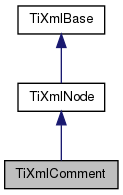
\includegraphics[width=164pt]{class_ti_xml_comment__inherit__graph}
\end{center}
\end{figure}


\-Collaboration diagram for \-Ti\-Xml\-Comment\-:\nopagebreak
\begin{figure}[H]
\begin{center}
\leavevmode
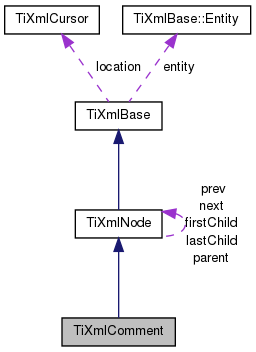
\includegraphics[width=264pt]{class_ti_xml_comment__coll__graph}
\end{center}
\end{figure}
\subsection*{\-Public \-Member \-Functions}
\begin{DoxyCompactItemize}
\item 
\hypertarget{class_ti_xml_comment_aaa3252031d3e8bd3a2bf51a1c61201b7}{\hyperlink{class_ti_xml_comment_aaa3252031d3e8bd3a2bf51a1c61201b7}{\-Ti\-Xml\-Comment} ()}\label{class_ti_xml_comment_aaa3252031d3e8bd3a2bf51a1c61201b7}

\begin{DoxyCompactList}\small\item\em \-Constructs an empty comment. \end{DoxyCompactList}\item 
\hypertarget{class_ti_xml_comment_a37e7802ef17bc03ebe5ae79bf0713d47}{\hyperlink{class_ti_xml_comment_a37e7802ef17bc03ebe5ae79bf0713d47}{\-Ti\-Xml\-Comment} (const char $\ast$\-\_\-value)}\label{class_ti_xml_comment_a37e7802ef17bc03ebe5ae79bf0713d47}

\begin{DoxyCompactList}\small\item\em \-Construct a comment from text. \end{DoxyCompactList}\item 
\hypertarget{class_ti_xml_comment_afaec41ac2760ce946ba1590eb5708e50}{{\bfseries \-Ti\-Xml\-Comment} (const \hyperlink{class_ti_xml_comment}{\-Ti\-Xml\-Comment} \&)}\label{class_ti_xml_comment_afaec41ac2760ce946ba1590eb5708e50}

\item 
\hypertarget{class_ti_xml_comment_aeceedc15f8b8f9ca0b6136696339b3ac}{\hyperlink{class_ti_xml_comment}{\-Ti\-Xml\-Comment} \& {\bfseries operator=} (const \hyperlink{class_ti_xml_comment}{\-Ti\-Xml\-Comment} \&base)}\label{class_ti_xml_comment_aeceedc15f8b8f9ca0b6136696339b3ac}

\item 
\hypertarget{class_ti_xml_comment_a4f6590c9c9a2b63a48972655b78eb853}{virtual \hyperlink{class_ti_xml_node}{\-Ti\-Xml\-Node} $\ast$ \hyperlink{class_ti_xml_comment_a4f6590c9c9a2b63a48972655b78eb853}{\-Clone} () const }\label{class_ti_xml_comment_a4f6590c9c9a2b63a48972655b78eb853}

\begin{DoxyCompactList}\small\item\em \-Returns a copy of this \-Comment. \end{DoxyCompactList}\item 
virtual void \hyperlink{class_ti_xml_comment_a17398061d62c470f57801ce28fa33ad4}{\-Print} (\-F\-I\-L\-E $\ast$cfile, int depth) const 
\item 
\hypertarget{class_ti_xml_comment_a43bddc18ac057734b41d84653b71d3e0}{virtual const char $\ast$ {\bfseries \-Parse} (const char $\ast$p, \hyperlink{class_ti_xml_parsing_data}{\-Ti\-Xml\-Parsing\-Data} $\ast$data, \-Ti\-Xml\-Encoding encoding)}\label{class_ti_xml_comment_a43bddc18ac057734b41d84653b71d3e0}

\item 
\hypertarget{class_ti_xml_comment_a00fb4215c20a2399ea05ac9b9e7e68a0}{virtual const \hyperlink{class_ti_xml_comment}{\-Ti\-Xml\-Comment} $\ast$ \hyperlink{class_ti_xml_comment_a00fb4215c20a2399ea05ac9b9e7e68a0}{\-To\-Comment} () const }\label{class_ti_xml_comment_a00fb4215c20a2399ea05ac9b9e7e68a0}

\begin{DoxyCompactList}\small\item\em \-Cast to a more defined type. \-Will return null not of the requested type. \end{DoxyCompactList}\item 
\hypertarget{class_ti_xml_comment_acc7c7e07e13c23f17797d642981511df}{virtual \hyperlink{class_ti_xml_comment}{\-Ti\-Xml\-Comment} $\ast$ \hyperlink{class_ti_xml_comment_acc7c7e07e13c23f17797d642981511df}{\-To\-Comment} ()}\label{class_ti_xml_comment_acc7c7e07e13c23f17797d642981511df}

\begin{DoxyCompactList}\small\item\em \-Cast to a more defined type. \-Will return null not of the requested type. \end{DoxyCompactList}\item 
virtual bool \hyperlink{class_ti_xml_comment_a4382de0e50da973f11a23ea5852568bd}{\-Accept} (\hyperlink{class_ti_xml_visitor}{\-Ti\-Xml\-Visitor} $\ast$visitor) const 
\end{DoxyCompactItemize}
\subsection*{\-Protected \-Member \-Functions}
\begin{DoxyCompactItemize}
\item 
\hypertarget{class_ti_xml_comment_a3175b2f27628f4fb7a043897930cd934}{void {\bfseries \-Copy\-To} (\hyperlink{class_ti_xml_comment}{\-Ti\-Xml\-Comment} $\ast$target) const }\label{class_ti_xml_comment_a3175b2f27628f4fb7a043897930cd934}

\end{DoxyCompactItemize}


\subsection{\-Detailed \-Description}
\-An \-X\-M\-L comment. 

\subsection{\-Member \-Function \-Documentation}
\hypertarget{class_ti_xml_comment_a4382de0e50da973f11a23ea5852568bd}{\index{\-Ti\-Xml\-Comment@{\-Ti\-Xml\-Comment}!\-Accept@{\-Accept}}
\index{\-Accept@{\-Accept}!TiXmlComment@{\-Ti\-Xml\-Comment}}
\subsubsection[{\-Accept}]{\setlength{\rightskip}{0pt plus 5cm}bool {\bf \-Ti\-Xml\-Comment\-::\-Accept} (
\begin{DoxyParamCaption}
\item[{{\bf \-Ti\-Xml\-Visitor} $\ast$}]{visitor}
\end{DoxyParamCaption}
) const\hspace{0.3cm}{\ttfamily  \mbox{[}virtual\mbox{]}}}}\label{class_ti_xml_comment_a4382de0e50da973f11a23ea5852568bd}
\-Walk the \-X\-M\-L tree visiting this node and all of its children. 

\-Implements \hyperlink{class_ti_xml_node_acc0f88b7462c6cb73809d410a4f5bb86}{\-Ti\-Xml\-Node}.

\hypertarget{class_ti_xml_comment_a17398061d62c470f57801ce28fa33ad4}{\index{\-Ti\-Xml\-Comment@{\-Ti\-Xml\-Comment}!\-Print@{\-Print}}
\index{\-Print@{\-Print}!TiXmlComment@{\-Ti\-Xml\-Comment}}
\subsubsection[{\-Print}]{\setlength{\rightskip}{0pt plus 5cm}void {\bf \-Ti\-Xml\-Comment\-::\-Print} (
\begin{DoxyParamCaption}
\item[{\-F\-I\-L\-E $\ast$}]{cfile, }
\item[{int}]{depth}
\end{DoxyParamCaption}
) const\hspace{0.3cm}{\ttfamily  \mbox{[}virtual\mbox{]}}}}\label{class_ti_xml_comment_a17398061d62c470f57801ce28fa33ad4}
\-All \-Tiny\-Xml classes can print themselves to a filestream or the string class (\hyperlink{class_ti_xml_string}{\-Ti\-Xml\-String} in non-\/\-S\-T\-L mode, std\-::string in \-S\-T\-L mode.) \-Either or both cfile and str can be null.

\-This is a formatted print, and will insert tabs and newlines.

(\-For an unformatted stream, use the $<$$<$ operator.) 

\-Implements \hyperlink{class_ti_xml_base_a0de56b3f2ef14c65091a3b916437b512}{\-Ti\-Xml\-Base}.



\-The documentation for this class was generated from the following files\-:\begin{DoxyCompactItemize}
\item 
tinyxml/tinyxml.\-h\item 
tinyxml/tinyxml.\-cpp\item 
tinyxml/tinyxmlparser.\-cpp\end{DoxyCompactItemize}

\hypertarget{struct_ti_xml_cursor}{\section{\-Ti\-Xml\-Cursor \-Struct \-Reference}
\label{struct_ti_xml_cursor}\index{\-Ti\-Xml\-Cursor@{\-Ti\-Xml\-Cursor}}
}
\subsection*{\-Public \-Member \-Functions}
\begin{DoxyCompactItemize}
\item 
\hypertarget{struct_ti_xml_cursor_a1e6fa622b59dafb71b6efe595105dcdd}{void {\bfseries \-Clear} ()}\label{struct_ti_xml_cursor_a1e6fa622b59dafb71b6efe595105dcdd}

\end{DoxyCompactItemize}
\subsection*{\-Public \-Attributes}
\begin{DoxyCompactItemize}
\item 
\hypertarget{struct_ti_xml_cursor_a5b54dd949820c2db061e2be41f3effb3}{int {\bfseries row}}\label{struct_ti_xml_cursor_a5b54dd949820c2db061e2be41f3effb3}

\item 
\hypertarget{struct_ti_xml_cursor_a5694d7ed2c4d20109d350c14c417969d}{int {\bfseries col}}\label{struct_ti_xml_cursor_a5694d7ed2c4d20109d350c14c417969d}

\end{DoxyCompactItemize}


\-The documentation for this struct was generated from the following file\-:\begin{DoxyCompactItemize}
\item 
tinyxml/tinyxml.\-h\end{DoxyCompactItemize}

\hypertarget{class_ti_xml_declaration}{\section{\-Ti\-Xml\-Declaration \-Class \-Reference}
\label{class_ti_xml_declaration}\index{\-Ti\-Xml\-Declaration@{\-Ti\-Xml\-Declaration}}
}


{\ttfamily \#include $<$tinyxml.\-h$>$}



\-Inheritance diagram for \-Ti\-Xml\-Declaration\-:
\nopagebreak
\begin{figure}[H]
\begin{center}
\leavevmode
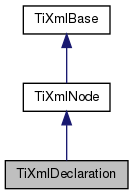
\includegraphics[width=172pt]{class_ti_xml_declaration__inherit__graph}
\end{center}
\end{figure}


\-Collaboration diagram for \-Ti\-Xml\-Declaration\-:
\nopagebreak
\begin{figure}[H]
\begin{center}
\leavevmode
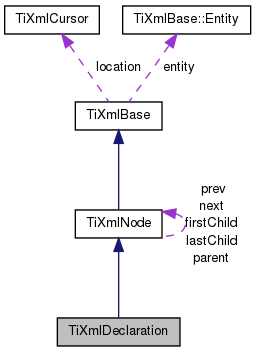
\includegraphics[width=216pt]{class_ti_xml_declaration__coll__graph}
\end{center}
\end{figure}
\subsection*{\-Public \-Member \-Functions}
\begin{DoxyCompactItemize}
\item 
\hypertarget{class_ti_xml_declaration_aa0484d059bea0ea1acb47c9094382d79}{\hyperlink{class_ti_xml_declaration_aa0484d059bea0ea1acb47c9094382d79}{\-Ti\-Xml\-Declaration} ()}\label{class_ti_xml_declaration_aa0484d059bea0ea1acb47c9094382d79}

\begin{DoxyCompactList}\small\item\em \-Construct an empty declaration. \end{DoxyCompactList}\item 
\hypertarget{class_ti_xml_declaration_a3b618d1c30c25e4b7a71f31a595ee298}{\hyperlink{class_ti_xml_declaration_a3b618d1c30c25e4b7a71f31a595ee298}{\-Ti\-Xml\-Declaration} (const char $\ast$\-\_\-version, const char $\ast$\-\_\-encoding, const char $\ast$\-\_\-standalone)}\label{class_ti_xml_declaration_a3b618d1c30c25e4b7a71f31a595ee298}

\begin{DoxyCompactList}\small\item\em \-Construct. \end{DoxyCompactList}\item 
\hypertarget{class_ti_xml_declaration_a58ac9042c342f7845c8491da0bb091e8}{{\bfseries \-Ti\-Xml\-Declaration} (const \hyperlink{class_ti_xml_declaration}{\-Ti\-Xml\-Declaration} \&copy)}\label{class_ti_xml_declaration_a58ac9042c342f7845c8491da0bb091e8}

\item 
\hypertarget{class_ti_xml_declaration_a3bc617efe11014ff2b1a9c5727c37a9a}{\hyperlink{class_ti_xml_declaration}{\-Ti\-Xml\-Declaration} \& {\bfseries operator=} (const \hyperlink{class_ti_xml_declaration}{\-Ti\-Xml\-Declaration} \&copy)}\label{class_ti_xml_declaration_a3bc617efe11014ff2b1a9c5727c37a9a}

\item 
\hypertarget{class_ti_xml_declaration_a02ee557b1a4545c3219ed377c103ec76}{const char $\ast$ \hyperlink{class_ti_xml_declaration_a02ee557b1a4545c3219ed377c103ec76}{\-Version} () const }\label{class_ti_xml_declaration_a02ee557b1a4545c3219ed377c103ec76}

\begin{DoxyCompactList}\small\item\em \-Version. \-Will return an empty string if none was found. \end{DoxyCompactList}\item 
\hypertarget{class_ti_xml_declaration_a5d974231f9e9a2f0542f15f3a46cdb76}{const char $\ast$ \hyperlink{class_ti_xml_declaration_a5d974231f9e9a2f0542f15f3a46cdb76}{\-Encoding} () const }\label{class_ti_xml_declaration_a5d974231f9e9a2f0542f15f3a46cdb76}

\begin{DoxyCompactList}\small\item\em \-Encoding. \-Will return an empty string if none was found. \end{DoxyCompactList}\item 
\hypertarget{class_ti_xml_declaration_a9ff06afc033d7ef730ec7c6825b97ad9}{const char $\ast$ \hyperlink{class_ti_xml_declaration_a9ff06afc033d7ef730ec7c6825b97ad9}{\-Standalone} () const }\label{class_ti_xml_declaration_a9ff06afc033d7ef730ec7c6825b97ad9}

\begin{DoxyCompactList}\small\item\em \-Is this a standalone document? \end{DoxyCompactList}\item 
\hypertarget{class_ti_xml_declaration_aff8231266d735943d8a7514a9c9822b9}{virtual \hyperlink{class_ti_xml_node}{\-Ti\-Xml\-Node} $\ast$ \hyperlink{class_ti_xml_declaration_aff8231266d735943d8a7514a9c9822b9}{\-Clone} () const }\label{class_ti_xml_declaration_aff8231266d735943d8a7514a9c9822b9}

\begin{DoxyCompactList}\small\item\em \-Creates a copy of this \-Declaration and returns it. \end{DoxyCompactList}\item 
\hypertarget{class_ti_xml_declaration_aa5ab32ec19d4eeecff4a9238c6c90565}{virtual void {\bfseries \-Print} (\-F\-I\-L\-E $\ast$cfile, int depth, \-T\-I\-X\-M\-L\-\_\-\-S\-T\-R\-I\-N\-G $\ast$str) const }\label{class_ti_xml_declaration_aa5ab32ec19d4eeecff4a9238c6c90565}

\item 
virtual void \hyperlink{class_ti_xml_declaration_abf6303db4bd05b5be554036817ff1cb4}{\-Print} (\-F\-I\-L\-E $\ast$cfile, int depth) const 
\item 
\hypertarget{class_ti_xml_declaration_a9839ea97ed687a2b7342fd7b0f04361b}{virtual const char $\ast$ {\bfseries \-Parse} (const char $\ast$p, \hyperlink{class_ti_xml_parsing_data}{\-Ti\-Xml\-Parsing\-Data} $\ast$data, \-Ti\-Xml\-Encoding encoding)}\label{class_ti_xml_declaration_a9839ea97ed687a2b7342fd7b0f04361b}

\item 
\hypertarget{class_ti_xml_declaration_a1e085d3fefd1dbf5ccdbff729931a967}{virtual const \hyperlink{class_ti_xml_declaration}{\-Ti\-Xml\-Declaration} $\ast$ \hyperlink{class_ti_xml_declaration_a1e085d3fefd1dbf5ccdbff729931a967}{\-To\-Declaration} () const }\label{class_ti_xml_declaration_a1e085d3fefd1dbf5ccdbff729931a967}

\begin{DoxyCompactList}\small\item\em \-Cast to a more defined type. \-Will return null not of the requested type. \end{DoxyCompactList}\item 
\hypertarget{class_ti_xml_declaration_a6bd3d1daddcaeb9543c24bfd090969ce}{virtual \hyperlink{class_ti_xml_declaration}{\-Ti\-Xml\-Declaration} $\ast$ \hyperlink{class_ti_xml_declaration_a6bd3d1daddcaeb9543c24bfd090969ce}{\-To\-Declaration} ()}\label{class_ti_xml_declaration_a6bd3d1daddcaeb9543c24bfd090969ce}

\begin{DoxyCompactList}\small\item\em \-Cast to a more defined type. \-Will return null not of the requested type. \end{DoxyCompactList}\item 
virtual bool \hyperlink{class_ti_xml_declaration_ab6a6b178161ba9abc2c35058de689864}{\-Accept} (\hyperlink{class_ti_xml_visitor}{\-Ti\-Xml\-Visitor} $\ast$visitor) const 
\end{DoxyCompactItemize}
\subsection*{\-Protected \-Member \-Functions}
\begin{DoxyCompactItemize}
\item 
\hypertarget{class_ti_xml_declaration_a9d08959f935421a593032bd3efb30c38}{void {\bfseries \-Copy\-To} (\hyperlink{class_ti_xml_declaration}{\-Ti\-Xml\-Declaration} $\ast$target) const }\label{class_ti_xml_declaration_a9d08959f935421a593032bd3efb30c38}

\end{DoxyCompactItemize}


\subsection{\-Detailed \-Description}
\-In correct \-X\-M\-L the declaration is the first entry in the file. \begin{DoxyVerb}
		<?xml version="1.0" standalone="yes"?>
	\end{DoxyVerb}


\-Tiny\-Xml will happily read or write files without a declaration, however. \-There are 3 possible attributes to the declaration\-: version, encoding, and standalone.

\-Note\-: \-In this version of the code, the attributes are handled as special cases, not generic attributes, simply because there can only be at most 3 and they are always the same. 

\subsection{\-Member \-Function \-Documentation}
\hypertarget{class_ti_xml_declaration_ab6a6b178161ba9abc2c35058de689864}{\index{\-Ti\-Xml\-Declaration@{\-Ti\-Xml\-Declaration}!\-Accept@{\-Accept}}
\index{\-Accept@{\-Accept}!TiXmlDeclaration@{\-Ti\-Xml\-Declaration}}
\subsubsection[{\-Accept}]{\setlength{\rightskip}{0pt plus 5cm}bool {\bf \-Ti\-Xml\-Declaration\-::\-Accept} (
\begin{DoxyParamCaption}
\item[{{\bf \-Ti\-Xml\-Visitor} $\ast$}]{visitor}
\end{DoxyParamCaption}
) const\hspace{0.3cm}{\ttfamily  \mbox{[}virtual\mbox{]}}}}\label{class_ti_xml_declaration_ab6a6b178161ba9abc2c35058de689864}
\-Walk the \-X\-M\-L tree visiting this node and all of its children. 

\-Implements \hyperlink{class_ti_xml_node_acc0f88b7462c6cb73809d410a4f5bb86}{\-Ti\-Xml\-Node}.

\hypertarget{class_ti_xml_declaration_abf6303db4bd05b5be554036817ff1cb4}{\index{\-Ti\-Xml\-Declaration@{\-Ti\-Xml\-Declaration}!\-Print@{\-Print}}
\index{\-Print@{\-Print}!TiXmlDeclaration@{\-Ti\-Xml\-Declaration}}
\subsubsection[{\-Print}]{\setlength{\rightskip}{0pt plus 5cm}virtual void \-Ti\-Xml\-Declaration\-::\-Print (
\begin{DoxyParamCaption}
\item[{\-F\-I\-L\-E $\ast$}]{cfile, }
\item[{int}]{depth}
\end{DoxyParamCaption}
) const\hspace{0.3cm}{\ttfamily  \mbox{[}inline, virtual\mbox{]}}}}\label{class_ti_xml_declaration_abf6303db4bd05b5be554036817ff1cb4}
\-All \-Tiny\-Xml classes can print themselves to a filestream or the string class (\hyperlink{class_ti_xml_string}{\-Ti\-Xml\-String} in non-\/\-S\-T\-L mode, std\-::string in \-S\-T\-L mode.) \-Either or both cfile and str can be null.

\-This is a formatted print, and will insert tabs and newlines.

(\-For an unformatted stream, use the $<$$<$ operator.) 

\-Implements \hyperlink{class_ti_xml_base_a0de56b3f2ef14c65091a3b916437b512}{\-Ti\-Xml\-Base}.



\-The documentation for this class was generated from the following files\-:\begin{DoxyCompactItemize}
\item 
tinyxml/tinyxml.\-h\item 
tinyxml/tinyxml.\-cpp\item 
tinyxml/tinyxmlparser.\-cpp\end{DoxyCompactItemize}

\hypertarget{class_ti_xml_document}{\section{\-Ti\-Xml\-Document \-Class \-Reference}
\label{class_ti_xml_document}\index{\-Ti\-Xml\-Document@{\-Ti\-Xml\-Document}}
}


{\ttfamily \#include $<$tinyxml.\-h$>$}



\-Inheritance diagram for \-Ti\-Xml\-Document\-:\nopagebreak
\begin{figure}[H]
\begin{center}
\leavevmode
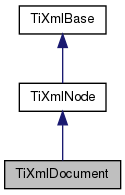
\includegraphics[width=166pt]{class_ti_xml_document__inherit__graph}
\end{center}
\end{figure}


\-Collaboration diagram for \-Ti\-Xml\-Document\-:
\nopagebreak
\begin{figure}[H]
\begin{center}
\leavevmode
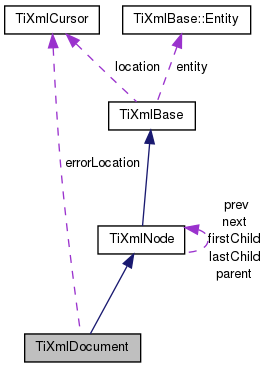
\includegraphics[width=272pt]{class_ti_xml_document__coll__graph}
\end{center}
\end{figure}
\subsection*{\-Public \-Member \-Functions}
\begin{DoxyCompactItemize}
\item 
\hypertarget{class_ti_xml_document_a9f5e84335708fde98400230f9f12659c}{\hyperlink{class_ti_xml_document_a9f5e84335708fde98400230f9f12659c}{\-Ti\-Xml\-Document} ()}\label{class_ti_xml_document_a9f5e84335708fde98400230f9f12659c}

\begin{DoxyCompactList}\small\item\em \-Create an empty document, that has no name. \end{DoxyCompactList}\item 
\hypertarget{class_ti_xml_document_ae4508b452d0c3061db085f3db27b8396}{\hyperlink{class_ti_xml_document_ae4508b452d0c3061db085f3db27b8396}{\-Ti\-Xml\-Document} (const char $\ast$document\-Name)}\label{class_ti_xml_document_ae4508b452d0c3061db085f3db27b8396}

\begin{DoxyCompactList}\small\item\em \-Create a document with a name. \-The name of the document is also the filename of the xml. \end{DoxyCompactList}\item 
\hypertarget{class_ti_xml_document_a323a7486e7da6099cdc19a5ff7e74b07}{{\bfseries \-Ti\-Xml\-Document} (const \hyperlink{class_ti_xml_document}{\-Ti\-Xml\-Document} \&copy)}\label{class_ti_xml_document_a323a7486e7da6099cdc19a5ff7e74b07}

\item 
\hypertarget{class_ti_xml_document_aa56fd4dbe8917d2033d865909e2d737e}{\hyperlink{class_ti_xml_document}{\-Ti\-Xml\-Document} \& {\bfseries operator=} (const \hyperlink{class_ti_xml_document}{\-Ti\-Xml\-Document} \&copy)}\label{class_ti_xml_document_aa56fd4dbe8917d2033d865909e2d737e}

\item 
bool \hyperlink{class_ti_xml_document_a4c852a889c02cf251117fd1d9fe1845f}{\-Load\-File} (\-Ti\-Xml\-Encoding encoding=\-T\-I\-X\-M\-L\-\_\-\-D\-E\-F\-A\-U\-L\-T\-\_\-\-E\-N\-C\-O\-D\-I\-N\-G)
\item 
\hypertarget{class_ti_xml_document_a21c0aeb0d0a720169ad4ac89523ebe93}{bool \hyperlink{class_ti_xml_document_a21c0aeb0d0a720169ad4ac89523ebe93}{\-Save\-File} () const }\label{class_ti_xml_document_a21c0aeb0d0a720169ad4ac89523ebe93}

\begin{DoxyCompactList}\small\item\em \-Save a file using the current document value. \-Returns true if successful. \end{DoxyCompactList}\item 
\hypertarget{class_ti_xml_document_a879cdf5e981b8b2d2ef82f2546dd28fb}{bool \hyperlink{class_ti_xml_document_a879cdf5e981b8b2d2ef82f2546dd28fb}{\-Load\-File} (const char $\ast$filename, \-Ti\-Xml\-Encoding encoding=\-T\-I\-X\-M\-L\-\_\-\-D\-E\-F\-A\-U\-L\-T\-\_\-\-E\-N\-C\-O\-D\-I\-N\-G)}\label{class_ti_xml_document_a879cdf5e981b8b2d2ef82f2546dd28fb}

\begin{DoxyCompactList}\small\item\em \-Load a file using the given filename. \-Returns true if successful. \end{DoxyCompactList}\item 
\hypertarget{class_ti_xml_document_ae869f5ebf7fc54c4a1d737fb4689fd44}{bool \hyperlink{class_ti_xml_document_ae869f5ebf7fc54c4a1d737fb4689fd44}{\-Save\-File} (const char $\ast$filename) const }\label{class_ti_xml_document_ae869f5ebf7fc54c4a1d737fb4689fd44}

\begin{DoxyCompactList}\small\item\em \-Save a file using the given filename. \-Returns true if successful. \end{DoxyCompactList}\item 
bool \hyperlink{class_ti_xml_document_a41f6fe7200864d1dca663d230caf8db6}{\-Load\-File} (\-F\-I\-L\-E $\ast$, \-Ti\-Xml\-Encoding encoding=\-T\-I\-X\-M\-L\-\_\-\-D\-E\-F\-A\-U\-L\-T\-\_\-\-E\-N\-C\-O\-D\-I\-N\-G)
\item 
\hypertarget{class_ti_xml_document_acf1672b4538c6d1d441f9f108aea2bf4}{bool \hyperlink{class_ti_xml_document_acf1672b4538c6d1d441f9f108aea2bf4}{\-Save\-File} (\-F\-I\-L\-E $\ast$) const }\label{class_ti_xml_document_acf1672b4538c6d1d441f9f108aea2bf4}

\begin{DoxyCompactList}\small\item\em \-Save a file using the given \-F\-I\-L\-E$\ast$. \-Returns true if successful. \end{DoxyCompactList}\item 
virtual const char $\ast$ \hyperlink{class_ti_xml_document_a789ad2f06f93d52bdb5570b2f3670289}{\-Parse} (const char $\ast$p, \hyperlink{class_ti_xml_parsing_data}{\-Ti\-Xml\-Parsing\-Data} $\ast$data=0, \-Ti\-Xml\-Encoding encoding=\-T\-I\-X\-M\-L\-\_\-\-D\-E\-F\-A\-U\-L\-T\-\_\-\-E\-N\-C\-O\-D\-I\-N\-G)
\item 
const \hyperlink{class_ti_xml_element}{\-Ti\-Xml\-Element} $\ast$ \hyperlink{class_ti_xml_document_ad09d17927f908f40efb406af2fb873be}{\-Root\-Element} () const 
\item 
\hypertarget{class_ti_xml_document_a0b43e762a23f938b06651bc90b8a1013}{\hyperlink{class_ti_xml_element}{\-Ti\-Xml\-Element} $\ast$ {\bfseries \-Root\-Element} ()}\label{class_ti_xml_document_a0b43e762a23f938b06651bc90b8a1013}

\item 
bool \hyperlink{class_ti_xml_document_a6dfc01a6e5d58e56acd537dfd3bdeb29}{\-Error} () const 
\item 
\hypertarget{class_ti_xml_document_a9d0f689f6e09ea494ea547be8d79c25e}{const char $\ast$ \hyperlink{class_ti_xml_document_a9d0f689f6e09ea494ea547be8d79c25e}{\-Error\-Desc} () const }\label{class_ti_xml_document_a9d0f689f6e09ea494ea547be8d79c25e}

\begin{DoxyCompactList}\small\item\em \-Contains a textual (english) description of the error if one occurs. \end{DoxyCompactList}\item 
int \hyperlink{class_ti_xml_document_af96fc2f3f9ec6422782bfe916c9e778f}{\-Error\-Id} () const 
\item 
int \hyperlink{class_ti_xml_document_af30efc75e804aa2e92fb8be3a8cb676e}{\-Error\-Row} () const 
\item 
\hypertarget{class_ti_xml_document_aa90bc630ee5203c6109ca5fad3323649}{int \hyperlink{class_ti_xml_document_aa90bc630ee5203c6109ca5fad3323649}{\-Error\-Col} () const }\label{class_ti_xml_document_aa90bc630ee5203c6109ca5fad3323649}

\begin{DoxyCompactList}\small\item\em \-The column where the error occured. \-See \hyperlink{class_ti_xml_document_af30efc75e804aa2e92fb8be3a8cb676e}{\-Error\-Row()} \end{DoxyCompactList}\item 
void \hyperlink{class_ti_xml_document_a51dac56316f89b35bdb7d0d433ba988e}{\-Set\-Tab\-Size} (int \-\_\-tabsize)
\item 
\hypertarget{class_ti_xml_document_a612360241b85bad0826b2a9ae9cda561}{int {\bfseries \-Tab\-Size} () const }\label{class_ti_xml_document_a612360241b85bad0826b2a9ae9cda561}

\item 
void \hyperlink{class_ti_xml_document_ac66b8c28db86363315712a3574e87c35}{\-Clear\-Error} ()
\item 
void \hyperlink{class_ti_xml_document_af08389ec70ee9b2de7f800e206a18510}{\-Print} () const 
\item 
\hypertarget{class_ti_xml_document_a7b1aea204fee266b70b9c105c8bf2ada}{virtual void \hyperlink{class_ti_xml_document_a7b1aea204fee266b70b9c105c8bf2ada}{\-Print} (\-F\-I\-L\-E $\ast$cfile, int depth=0) const }\label{class_ti_xml_document_a7b1aea204fee266b70b9c105c8bf2ada}

\begin{DoxyCompactList}\small\item\em \-Print this \-Document to a \-F\-I\-L\-E stream. \end{DoxyCompactList}\item 
\hypertarget{class_ti_xml_document_a735c23e318597b920c94eae77fa206de}{void {\bfseries \-Set\-Error} (int err, const char $\ast$error\-Location, \hyperlink{class_ti_xml_parsing_data}{\-Ti\-Xml\-Parsing\-Data} $\ast$prev\-Data, \-Ti\-Xml\-Encoding encoding)}\label{class_ti_xml_document_a735c23e318597b920c94eae77fa206de}

\item 
\hypertarget{class_ti_xml_document_a1dc977bde3e4fe85a8eb9d88a35ef5a4}{virtual const \hyperlink{class_ti_xml_document}{\-Ti\-Xml\-Document} $\ast$ \hyperlink{class_ti_xml_document_a1dc977bde3e4fe85a8eb9d88a35ef5a4}{\-To\-Document} () const }\label{class_ti_xml_document_a1dc977bde3e4fe85a8eb9d88a35ef5a4}

\begin{DoxyCompactList}\small\item\em \-Cast to a more defined type. \-Will return null not of the requested type. \end{DoxyCompactList}\item 
\hypertarget{class_ti_xml_document_a1025d942a1f328fd742d545e37efdd42}{virtual \hyperlink{class_ti_xml_document}{\-Ti\-Xml\-Document} $\ast$ \hyperlink{class_ti_xml_document_a1025d942a1f328fd742d545e37efdd42}{\-To\-Document} ()}\label{class_ti_xml_document_a1025d942a1f328fd742d545e37efdd42}

\begin{DoxyCompactList}\small\item\em \-Cast to a more defined type. \-Will return null not of the requested type. \end{DoxyCompactList}\item 
virtual bool \hyperlink{class_ti_xml_document_a3daab2f472418ef66315750202f762ae}{\-Accept} (\hyperlink{class_ti_xml_visitor}{\-Ti\-Xml\-Visitor} $\ast$content) const 
\end{DoxyCompactItemize}
\subsection*{\-Protected \-Member \-Functions}
\begin{DoxyCompactItemize}
\item 
virtual \hyperlink{class_ti_xml_node}{\-Ti\-Xml\-Node} $\ast$ \hyperlink{class_ti_xml_document_ac9e8f09b23454d953b32d1b65cd1409e}{\-Clone} () const 
\end{DoxyCompactItemize}
\subsection*{\-Private \-Member \-Functions}
\begin{DoxyCompactItemize}
\item 
\hypertarget{class_ti_xml_document_af69deeb984e060bd00f668460dec8ef2}{void {\bfseries \-Copy\-To} (\hyperlink{class_ti_xml_document}{\-Ti\-Xml\-Document} $\ast$target) const }\label{class_ti_xml_document_af69deeb984e060bd00f668460dec8ef2}

\end{DoxyCompactItemize}
\subsection*{\-Private \-Attributes}
\begin{DoxyCompactItemize}
\item 
\hypertarget{class_ti_xml_document_a1ff6a063602f31acae6f37fc049d8bbd}{bool {\bfseries error}}\label{class_ti_xml_document_a1ff6a063602f31acae6f37fc049d8bbd}

\item 
\hypertarget{class_ti_xml_document_acdef97a4bb80729ac6863dd54cee7eeb}{int {\bfseries error\-Id}}\label{class_ti_xml_document_acdef97a4bb80729ac6863dd54cee7eeb}

\item 
\hypertarget{class_ti_xml_document_a2da9a95ba3f9c895a8d7f4de7122a642}{\-T\-I\-X\-M\-L\-\_\-\-S\-T\-R\-I\-N\-G {\bfseries error\-Desc}}\label{class_ti_xml_document_a2da9a95ba3f9c895a8d7f4de7122a642}

\item 
\hypertarget{class_ti_xml_document_af2fa6a010b903d893d52cc6fee5575a1}{int {\bfseries tabsize}}\label{class_ti_xml_document_af2fa6a010b903d893d52cc6fee5575a1}

\item 
\hypertarget{class_ti_xml_document_aa4030f989f1549f6b897147fc2851d1a}{\hyperlink{struct_ti_xml_cursor}{\-Ti\-Xml\-Cursor} {\bfseries error\-Location}}\label{class_ti_xml_document_aa4030f989f1549f6b897147fc2851d1a}

\item 
\hypertarget{class_ti_xml_document_a4d5400dec9bfb55c640428de33297886}{bool {\bfseries use\-Microsoft\-B\-O\-M}}\label{class_ti_xml_document_a4d5400dec9bfb55c640428de33297886}

\end{DoxyCompactItemize}


\subsection{\-Detailed \-Description}
\-Always the top level node. \-A document binds together all the \-X\-M\-L pieces. \-It can be saved, loaded, and printed to the screen. \-The 'value' of a document node is the xml file name. 

\subsection{\-Member \-Function \-Documentation}
\hypertarget{class_ti_xml_document_a3daab2f472418ef66315750202f762ae}{\index{\-Ti\-Xml\-Document@{\-Ti\-Xml\-Document}!\-Accept@{\-Accept}}
\index{\-Accept@{\-Accept}!TiXmlDocument@{\-Ti\-Xml\-Document}}
\subsubsection[{\-Accept}]{\setlength{\rightskip}{0pt plus 5cm}bool {\bf \-Ti\-Xml\-Document\-::\-Accept} (
\begin{DoxyParamCaption}
\item[{{\bf \-Ti\-Xml\-Visitor} $\ast$}]{content}
\end{DoxyParamCaption}
) const\hspace{0.3cm}{\ttfamily  \mbox{[}virtual\mbox{]}}}}\label{class_ti_xml_document_a3daab2f472418ef66315750202f762ae}
\-Walk the \-X\-M\-L tree visiting this node and all of its children. 

\-Implements \hyperlink{class_ti_xml_node_acc0f88b7462c6cb73809d410a4f5bb86}{\-Ti\-Xml\-Node}.

\hypertarget{class_ti_xml_document_ac66b8c28db86363315712a3574e87c35}{\index{\-Ti\-Xml\-Document@{\-Ti\-Xml\-Document}!\-Clear\-Error@{\-Clear\-Error}}
\index{\-Clear\-Error@{\-Clear\-Error}!TiXmlDocument@{\-Ti\-Xml\-Document}}
\subsubsection[{\-Clear\-Error}]{\setlength{\rightskip}{0pt plus 5cm}void {\bf \-Ti\-Xml\-Document\-::\-Clear\-Error} (
\begin{DoxyParamCaption}
{}
\end{DoxyParamCaption}
)\hspace{0.3cm}{\ttfamily  \mbox{[}inline\mbox{]}}}}\label{class_ti_xml_document_ac66b8c28db86363315712a3574e87c35}
\-If you have handled the error, it can be reset with this call. \-The error state is automatically cleared if you \-Parse a new \-X\-M\-L block. \hypertarget{class_ti_xml_document_ac9e8f09b23454d953b32d1b65cd1409e}{\index{\-Ti\-Xml\-Document@{\-Ti\-Xml\-Document}!\-Clone@{\-Clone}}
\index{\-Clone@{\-Clone}!TiXmlDocument@{\-Ti\-Xml\-Document}}
\subsubsection[{\-Clone}]{\setlength{\rightskip}{0pt plus 5cm}{\bf \-Ti\-Xml\-Node} $\ast$ {\bf \-Ti\-Xml\-Document\-::\-Clone} (
\begin{DoxyParamCaption}
{}
\end{DoxyParamCaption}
) const\hspace{0.3cm}{\ttfamily  \mbox{[}protected, virtual\mbox{]}}}}\label{class_ti_xml_document_ac9e8f09b23454d953b32d1b65cd1409e}
\-Create an exact duplicate of this node and return it. \-The memory must be deleted by the caller. 

\-Implements \hyperlink{class_ti_xml_node_a4508cc3a2d7a98e96a54cc09c37a78a4}{\-Ti\-Xml\-Node}.

\hypertarget{class_ti_xml_document_a6dfc01a6e5d58e56acd537dfd3bdeb29}{\index{\-Ti\-Xml\-Document@{\-Ti\-Xml\-Document}!\-Error@{\-Error}}
\index{\-Error@{\-Error}!TiXmlDocument@{\-Ti\-Xml\-Document}}
\subsubsection[{\-Error}]{\setlength{\rightskip}{0pt plus 5cm}bool {\bf \-Ti\-Xml\-Document\-::\-Error} (
\begin{DoxyParamCaption}
{}
\end{DoxyParamCaption}
) const\hspace{0.3cm}{\ttfamily  \mbox{[}inline\mbox{]}}}}\label{class_ti_xml_document_a6dfc01a6e5d58e56acd537dfd3bdeb29}
\-If an error occurs, \-Error will be set to true. \-Also,
\begin{DoxyItemize}
\item \-The \hyperlink{class_ti_xml_document_af96fc2f3f9ec6422782bfe916c9e778f}{\-Error\-Id()} will contain the integer identifier of the error (not generally useful)
\item \-The \hyperlink{class_ti_xml_document_a9d0f689f6e09ea494ea547be8d79c25e}{\-Error\-Desc()} method will return the name of the error. (very useful)
\item \-The \hyperlink{class_ti_xml_document_af30efc75e804aa2e92fb8be3a8cb676e}{\-Error\-Row()} and \hyperlink{class_ti_xml_document_aa90bc630ee5203c6109ca5fad3323649}{\-Error\-Col()} will return the location of the error (if known) 
\end{DoxyItemize}\hypertarget{class_ti_xml_document_af96fc2f3f9ec6422782bfe916c9e778f}{\index{\-Ti\-Xml\-Document@{\-Ti\-Xml\-Document}!\-Error\-Id@{\-Error\-Id}}
\index{\-Error\-Id@{\-Error\-Id}!TiXmlDocument@{\-Ti\-Xml\-Document}}
\subsubsection[{\-Error\-Id}]{\setlength{\rightskip}{0pt plus 5cm}int {\bf \-Ti\-Xml\-Document\-::\-Error\-Id} (
\begin{DoxyParamCaption}
{}
\end{DoxyParamCaption}
) const\hspace{0.3cm}{\ttfamily  \mbox{[}inline\mbox{]}}}}\label{class_ti_xml_document_af96fc2f3f9ec6422782bfe916c9e778f}
\-Generally, you probably want the error string ( \hyperlink{class_ti_xml_document_a9d0f689f6e09ea494ea547be8d79c25e}{\-Error\-Desc()} ). \-But if you prefer the \-Error\-Id, this function will fetch it. \hypertarget{class_ti_xml_document_af30efc75e804aa2e92fb8be3a8cb676e}{\index{\-Ti\-Xml\-Document@{\-Ti\-Xml\-Document}!\-Error\-Row@{\-Error\-Row}}
\index{\-Error\-Row@{\-Error\-Row}!TiXmlDocument@{\-Ti\-Xml\-Document}}
\subsubsection[{\-Error\-Row}]{\setlength{\rightskip}{0pt plus 5cm}int {\bf \-Ti\-Xml\-Document\-::\-Error\-Row} (
\begin{DoxyParamCaption}
{}
\end{DoxyParamCaption}
) const\hspace{0.3cm}{\ttfamily  \mbox{[}inline\mbox{]}}}}\label{class_ti_xml_document_af30efc75e804aa2e92fb8be3a8cb676e}
\-Returns the location (if known) of the error. \-The first column is column 1, and the first row is row 1. \-A value of 0 means the row and column wasn't applicable (memory errors, for example, have no row/column) or the parser lost the error. (\-An error in the error reporting, in that case.)

\begin{DoxySeeAlso}{\-See also}
\hyperlink{class_ti_xml_document_a51dac56316f89b35bdb7d0d433ba988e}{\-Set\-Tab\-Size}, \hyperlink{class_ti_xml_base_a024bceb070188df92c2a8d8852dd0853}{\-Row}, \hyperlink{class_ti_xml_base_ab54bfb9b70fe6dd276e7b279cab7f003}{\-Column} 
\end{DoxySeeAlso}
\hypertarget{class_ti_xml_document_a4c852a889c02cf251117fd1d9fe1845f}{\index{\-Ti\-Xml\-Document@{\-Ti\-Xml\-Document}!\-Load\-File@{\-Load\-File}}
\index{\-Load\-File@{\-Load\-File}!TiXmlDocument@{\-Ti\-Xml\-Document}}
\subsubsection[{\-Load\-File}]{\setlength{\rightskip}{0pt plus 5cm}bool {\bf \-Ti\-Xml\-Document\-::\-Load\-File} (
\begin{DoxyParamCaption}
\item[{\-Ti\-Xml\-Encoding}]{encoding = {\ttfamily \-T\-I\-X\-M\-L\-\_\-\-D\-E\-F\-A\-U\-L\-T\-\_\-\-E\-N\-C\-O\-D\-I\-N\-G}}
\end{DoxyParamCaption}
)}}\label{class_ti_xml_document_a4c852a889c02cf251117fd1d9fe1845f}
\-Load a file using the current document value. \-Returns true if successful. \-Will delete any existing document data before loading. \hypertarget{class_ti_xml_document_a41f6fe7200864d1dca663d230caf8db6}{\index{\-Ti\-Xml\-Document@{\-Ti\-Xml\-Document}!\-Load\-File@{\-Load\-File}}
\index{\-Load\-File@{\-Load\-File}!TiXmlDocument@{\-Ti\-Xml\-Document}}
\subsubsection[{\-Load\-File}]{\setlength{\rightskip}{0pt plus 5cm}bool {\bf \-Ti\-Xml\-Document\-::\-Load\-File} (
\begin{DoxyParamCaption}
\item[{\-F\-I\-L\-E $\ast$}]{file, }
\item[{\-Ti\-Xml\-Encoding}]{encoding = {\ttfamily \-T\-I\-X\-M\-L\-\_\-\-D\-E\-F\-A\-U\-L\-T\-\_\-\-E\-N\-C\-O\-D\-I\-N\-G}}
\end{DoxyParamCaption}
)}}\label{class_ti_xml_document_a41f6fe7200864d1dca663d230caf8db6}
\-Load a file using the given \-F\-I\-L\-E$\ast$. \-Returns true if successful. \-Note that this method doesn't stream -\/ the entire object pointed at by the \-F\-I\-L\-E$\ast$ will be interpreted as an \-X\-M\-L file. \-Tiny\-X\-M\-L doesn't stream in \-X\-M\-L from the current file location. \-Streaming may be added in the future. \hypertarget{class_ti_xml_document_a789ad2f06f93d52bdb5570b2f3670289}{\index{\-Ti\-Xml\-Document@{\-Ti\-Xml\-Document}!\-Parse@{\-Parse}}
\index{\-Parse@{\-Parse}!TiXmlDocument@{\-Ti\-Xml\-Document}}
\subsubsection[{\-Parse}]{\setlength{\rightskip}{0pt plus 5cm}const char $\ast$ {\bf \-Ti\-Xml\-Document\-::\-Parse} (
\begin{DoxyParamCaption}
\item[{const char $\ast$}]{p, }
\item[{{\bf \-Ti\-Xml\-Parsing\-Data} $\ast$}]{data = {\ttfamily 0}, }
\item[{\-Ti\-Xml\-Encoding}]{encoding = {\ttfamily \-T\-I\-X\-M\-L\-\_\-\-D\-E\-F\-A\-U\-L\-T\-\_\-\-E\-N\-C\-O\-D\-I\-N\-G}}
\end{DoxyParamCaption}
)\hspace{0.3cm}{\ttfamily  \mbox{[}virtual\mbox{]}}}}\label{class_ti_xml_document_a789ad2f06f93d52bdb5570b2f3670289}
\-Parse the given null terminated block of xml data. \-Passing in an encoding to this method (either \-T\-I\-X\-M\-L\-\_\-\-E\-N\-C\-O\-D\-I\-N\-G\-\_\-\-L\-E\-G\-A\-C\-Y or \-T\-I\-X\-M\-L\-\_\-\-E\-N\-C\-O\-D\-I\-N\-G\-\_\-\-U\-T\-F8 will force \-Tiny\-Xml to use that encoding, regardless of what \-Tiny\-Xml might otherwise try to detect. 

\-Implements \hyperlink{class_ti_xml_base}{\-Ti\-Xml\-Base}.

\hypertarget{class_ti_xml_document_af08389ec70ee9b2de7f800e206a18510}{\index{\-Ti\-Xml\-Document@{\-Ti\-Xml\-Document}!\-Print@{\-Print}}
\index{\-Print@{\-Print}!TiXmlDocument@{\-Ti\-Xml\-Document}}
\subsubsection[{\-Print}]{\setlength{\rightskip}{0pt plus 5cm}void {\bf \-Ti\-Xml\-Document\-::\-Print} (
\begin{DoxyParamCaption}
{}
\end{DoxyParamCaption}
) const\hspace{0.3cm}{\ttfamily  \mbox{[}inline\mbox{]}}}}\label{class_ti_xml_document_af08389ec70ee9b2de7f800e206a18510}
\-Write the document to standard out using formatted printing (\char`\"{}pretty print\char`\"{}). \hypertarget{class_ti_xml_document_ad09d17927f908f40efb406af2fb873be}{\index{\-Ti\-Xml\-Document@{\-Ti\-Xml\-Document}!\-Root\-Element@{\-Root\-Element}}
\index{\-Root\-Element@{\-Root\-Element}!TiXmlDocument@{\-Ti\-Xml\-Document}}
\subsubsection[{\-Root\-Element}]{\setlength{\rightskip}{0pt plus 5cm}const {\bf \-Ti\-Xml\-Element}$\ast$ {\bf \-Ti\-Xml\-Document\-::\-Root\-Element} (
\begin{DoxyParamCaption}
{}
\end{DoxyParamCaption}
) const\hspace{0.3cm}{\ttfamily  \mbox{[}inline\mbox{]}}}}\label{class_ti_xml_document_ad09d17927f908f40efb406af2fb873be}
\-Get the root element -\/-\/ the only top level element -\/-\/ of the document. \-In well formed \-X\-M\-L, there should only be one. \-Tiny\-Xml is tolerant of multiple elements at the document level. \hypertarget{class_ti_xml_document_a51dac56316f89b35bdb7d0d433ba988e}{\index{\-Ti\-Xml\-Document@{\-Ti\-Xml\-Document}!\-Set\-Tab\-Size@{\-Set\-Tab\-Size}}
\index{\-Set\-Tab\-Size@{\-Set\-Tab\-Size}!TiXmlDocument@{\-Ti\-Xml\-Document}}
\subsubsection[{\-Set\-Tab\-Size}]{\setlength{\rightskip}{0pt plus 5cm}void {\bf \-Ti\-Xml\-Document\-::\-Set\-Tab\-Size} (
\begin{DoxyParamCaption}
\item[{int}]{\-\_\-tabsize}
\end{DoxyParamCaption}
)\hspace{0.3cm}{\ttfamily  \mbox{[}inline\mbox{]}}}}\label{class_ti_xml_document_a51dac56316f89b35bdb7d0d433ba988e}
\hyperlink{class_ti_xml_document_a51dac56316f89b35bdb7d0d433ba988e}{\-Set\-Tab\-Size()} allows the error reporting functions (\hyperlink{class_ti_xml_document_af30efc75e804aa2e92fb8be3a8cb676e}{\-Error\-Row()} and \hyperlink{class_ti_xml_document_aa90bc630ee5203c6109ca5fad3323649}{\-Error\-Col()}) to report the correct values for row and column. \-It does not change the output or input in any way.

\-By calling this method, with a tab size greater than 0, the row and column of each node and attribute is stored when the file is loaded. \-Very useful for tracking the \-D\-O\-M back in to the source file.

\-The tab size is required for calculating the location of nodes. \-If not set, the default of 4 is used. \-The tabsize is set per document. \-Setting the tabsize to 0 disables row/column tracking.

\-Note that row and column tracking is not supported when using operator$>$$>$.

\-The tab size needs to be enabled before the parse or load. \-Correct usage\-: \begin{DoxyVerb}
		TiXmlDocument doc;
		doc.SetTabSize( 8 );
		doc.Load( "myfile.xml" );
		\end{DoxyVerb}


\begin{DoxySeeAlso}{\-See also}
\hyperlink{class_ti_xml_base_a024bceb070188df92c2a8d8852dd0853}{\-Row}, \hyperlink{class_ti_xml_base_ab54bfb9b70fe6dd276e7b279cab7f003}{\-Column} 
\end{DoxySeeAlso}


\-The documentation for this class was generated from the following files\-:\begin{DoxyCompactItemize}
\item 
tinyxml/tinyxml.\-h\item 
tinyxml/tinyxml.\-cpp\item 
tinyxml/tinyxmlparser.\-cpp\end{DoxyCompactItemize}

\hypertarget{class_ti_xml_element}{\section{\-Ti\-Xml\-Element \-Class \-Reference}
\label{class_ti_xml_element}\index{\-Ti\-Xml\-Element@{\-Ti\-Xml\-Element}}
}


{\ttfamily \#include $<$tinyxml.\-h$>$}



\-Inheritance diagram for \-Ti\-Xml\-Element\-:
\nopagebreak
\begin{figure}[H]
\begin{center}
\leavevmode
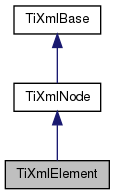
\includegraphics[width=158pt]{class_ti_xml_element__inherit__graph}
\end{center}
\end{figure}


\-Collaboration diagram for \-Ti\-Xml\-Element\-:
\nopagebreak
\begin{figure}[H]
\begin{center}
\leavevmode
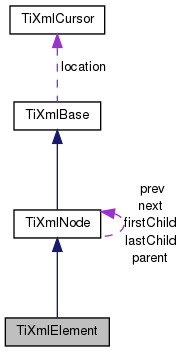
\includegraphics[width=209pt]{class_ti_xml_element__coll__graph}
\end{center}
\end{figure}
\subsection*{\-Public \-Member \-Functions}
\begin{DoxyCompactItemize}
\item 
\hypertarget{class_ti_xml_element_a01bc3ab372d35da08efcbbe65ad90c60}{\hyperlink{class_ti_xml_element_a01bc3ab372d35da08efcbbe65ad90c60}{\-Ti\-Xml\-Element} (const char $\ast$in\-\_\-value)}\label{class_ti_xml_element_a01bc3ab372d35da08efcbbe65ad90c60}

\begin{DoxyCompactList}\small\item\em \-Construct an element. \end{DoxyCompactList}\item 
\hypertarget{class_ti_xml_element_a1ca4465f3c2eac6a60e641cd7f1d9f7e}{{\bfseries \-Ti\-Xml\-Element} (const \hyperlink{class_ti_xml_element}{\-Ti\-Xml\-Element} \&)}\label{class_ti_xml_element_a1ca4465f3c2eac6a60e641cd7f1d9f7e}

\item 
\hypertarget{class_ti_xml_element_ad58d300f4cfc0016ffa6861ebb718a0b}{\hyperlink{class_ti_xml_element}{\-Ti\-Xml\-Element} \& {\bfseries operator=} (const \hyperlink{class_ti_xml_element}{\-Ti\-Xml\-Element} \&base)}\label{class_ti_xml_element_ad58d300f4cfc0016ffa6861ebb718a0b}

\item 
const char $\ast$ \hyperlink{class_ti_xml_element_ac1e4691e9375ba4e665dce7e46a50a9c}{\-Attribute} (const char $\ast$name) const 
\item 
const char $\ast$ \hyperlink{class_ti_xml_element_aa9192e80567b5042dbded80b78c44339}{\-Attribute} (const char $\ast$name, int $\ast$i) const 
\item 
const char $\ast$ \hyperlink{class_ti_xml_element_aec4f727f8aa49b51248d80125d173136}{\-Attribute} (const char $\ast$name, double $\ast$d) const 
\item 
int \hyperlink{class_ti_xml_element_aea0bfe471380f281c5945770ddbf52b9}{\-Query\-Int\-Attribute} (const char $\ast$name, int $\ast$\-\_\-value) const 
\item 
\hypertarget{class_ti_xml_element_ae48df644f890ab86fa19839ac401f00d}{int \hyperlink{class_ti_xml_element_ae48df644f890ab86fa19839ac401f00d}{\-Query\-Unsigned\-Attribute} (const char $\ast$name, unsigned $\ast$\-\_\-value) const }\label{class_ti_xml_element_ae48df644f890ab86fa19839ac401f00d}

\begin{DoxyCompactList}\small\item\em \-Query\-Unsigned\-Attribute examines the attribute -\/ see \hyperlink{class_ti_xml_element_aea0bfe471380f281c5945770ddbf52b9}{\-Query\-Int\-Attribute()}. \end{DoxyCompactList}\item 
int \hyperlink{class_ti_xml_element_af4a1d3f88c28eb0f3115dc39ebd83fff}{\-Query\-Bool\-Attribute} (const char $\ast$name, bool $\ast$\-\_\-value) const 
\item 
\hypertarget{class_ti_xml_element_a898d7730ecc341f0bffc7a9dadbf1ce7}{int \hyperlink{class_ti_xml_element_a898d7730ecc341f0bffc7a9dadbf1ce7}{\-Query\-Double\-Attribute} (const char $\ast$name, double $\ast$\-\_\-value) const }\label{class_ti_xml_element_a898d7730ecc341f0bffc7a9dadbf1ce7}

\begin{DoxyCompactList}\small\item\em \-Query\-Double\-Attribute examines the attribute -\/ see \hyperlink{class_ti_xml_element_aea0bfe471380f281c5945770ddbf52b9}{\-Query\-Int\-Attribute()}. \end{DoxyCompactList}\item 
\hypertarget{class_ti_xml_element_aa04d3af11601ef5a5f88295203a843be}{int \hyperlink{class_ti_xml_element_aa04d3af11601ef5a5f88295203a843be}{\-Query\-Float\-Attribute} (const char $\ast$name, float $\ast$\-\_\-value) const }\label{class_ti_xml_element_aa04d3af11601ef5a5f88295203a843be}

\begin{DoxyCompactList}\small\item\em \-Query\-Float\-Attribute examines the attribute -\/ see \hyperlink{class_ti_xml_element_aea0bfe471380f281c5945770ddbf52b9}{\-Query\-Int\-Attribute()}. \end{DoxyCompactList}\item 
void \hyperlink{class_ti_xml_element_abf0b3bd7f0e4c746a89ec6e7f101fc32}{\-Set\-Attribute} (const char $\ast$name, const char $\ast$\-\_\-value)
\item 
void \hyperlink{class_ti_xml_element_ace6f4be75e373726d4774073d666d1a7}{\-Set\-Attribute} (const char $\ast$name, int value)
\item 
void \hyperlink{class_ti_xml_element_a0d1dd975d75496778177e35abfe0ec0b}{\-Set\-Double\-Attribute} (const char $\ast$name, double value)
\item 
void \hyperlink{class_ti_xml_element_a56979767deca794376b1dfa69a525b2a}{\-Remove\-Attribute} (const char $\ast$name)
\item 
\hypertarget{class_ti_xml_element_a516054c9073647d6cb29b6abe9fa0592}{const \hyperlink{class_ti_xml_attribute}{\-Ti\-Xml\-Attribute} $\ast$ \hyperlink{class_ti_xml_element_a516054c9073647d6cb29b6abe9fa0592}{\-First\-Attribute} () const }\label{class_ti_xml_element_a516054c9073647d6cb29b6abe9fa0592}

\begin{DoxyCompactList}\small\item\em \-Access the first attribute in this element. \end{DoxyCompactList}\item 
\hypertarget{class_ti_xml_element_a4b33780fc565d38d6b54f640e0cf1737}{\hyperlink{class_ti_xml_attribute}{\-Ti\-Xml\-Attribute} $\ast$ {\bfseries \-First\-Attribute} ()}\label{class_ti_xml_element_a4b33780fc565d38d6b54f640e0cf1737}

\item 
\hypertarget{class_ti_xml_element_a86191b49f9177be132b85b14655f1381}{const \hyperlink{class_ti_xml_attribute}{\-Ti\-Xml\-Attribute} $\ast$ \hyperlink{class_ti_xml_element_a86191b49f9177be132b85b14655f1381}{\-Last\-Attribute} () const }\label{class_ti_xml_element_a86191b49f9177be132b85b14655f1381}

\begin{DoxyCompactList}\small\item\em \-Access the last attribute in this element. \end{DoxyCompactList}\item 
\hypertarget{class_ti_xml_element_a222f81cf06155cd108f2a68d4d176004}{\hyperlink{class_ti_xml_attribute}{\-Ti\-Xml\-Attribute} $\ast$ {\bfseries \-Last\-Attribute} ()}\label{class_ti_xml_element_a222f81cf06155cd108f2a68d4d176004}

\item 
const char $\ast$ \hyperlink{class_ti_xml_element_aa6dedd8a146acf3b1bc0903deb2d411a}{\-Get\-Text} () const 
\item 
\hypertarget{class_ti_xml_element_a13f6df105ebb1e8dc636e75cc883be32}{virtual \hyperlink{class_ti_xml_node}{\-Ti\-Xml\-Node} $\ast$ \hyperlink{class_ti_xml_element_a13f6df105ebb1e8dc636e75cc883be32}{\-Clone} () const }\label{class_ti_xml_element_a13f6df105ebb1e8dc636e75cc883be32}

\begin{DoxyCompactList}\small\item\em \-Creates a new \-Element and returns it -\/ the returned element is a copy. \end{DoxyCompactList}\item 
virtual void \hyperlink{class_ti_xml_element_ad9d0c008866982ab8d9aafae7e14d692}{\-Print} (\-F\-I\-L\-E $\ast$cfile, int depth) const 
\item 
\hypertarget{class_ti_xml_element_af95c9165159fd9dfdcc5b894a3fcf85b}{virtual const char $\ast$ {\bfseries \-Parse} (const char $\ast$p, \hyperlink{class_ti_xml_parsing_data}{\-Ti\-Xml\-Parsing\-Data} $\ast$data, \-Ti\-Xml\-Encoding encoding)}\label{class_ti_xml_element_af95c9165159fd9dfdcc5b894a3fcf85b}

\item 
\hypertarget{class_ti_xml_element_ac5b8d0e25fa23fd9acbb6d146082901c}{virtual const \hyperlink{class_ti_xml_element}{\-Ti\-Xml\-Element} $\ast$ \hyperlink{class_ti_xml_element_ac5b8d0e25fa23fd9acbb6d146082901c}{\-To\-Element} () const }\label{class_ti_xml_element_ac5b8d0e25fa23fd9acbb6d146082901c}

\begin{DoxyCompactList}\small\item\em \-Cast to a more defined type. \-Will return null not of the requested type. \end{DoxyCompactList}\item 
\hypertarget{class_ti_xml_element_a9def86337ea7a755eb41cac980f60c7a}{virtual \hyperlink{class_ti_xml_element}{\-Ti\-Xml\-Element} $\ast$ \hyperlink{class_ti_xml_element_a9def86337ea7a755eb41cac980f60c7a}{\-To\-Element} ()}\label{class_ti_xml_element_a9def86337ea7a755eb41cac980f60c7a}

\begin{DoxyCompactList}\small\item\em \-Cast to a more defined type. \-Will return null not of the requested type. \end{DoxyCompactList}\item 
virtual bool \hyperlink{class_ti_xml_element_a31ab28cc3b892a69254391d6bbe08df3}{\-Accept} (\hyperlink{class_ti_xml_visitor}{\-Ti\-Xml\-Visitor} $\ast$visitor) const 
\end{DoxyCompactItemize}
\subsection*{\-Protected \-Member \-Functions}
\begin{DoxyCompactItemize}
\item 
\hypertarget{class_ti_xml_element_a9e0c1983b840de4134f1f6bf7af00b0f}{void {\bfseries \-Copy\-To} (\hyperlink{class_ti_xml_element}{\-Ti\-Xml\-Element} $\ast$target) const }\label{class_ti_xml_element_a9e0c1983b840de4134f1f6bf7af00b0f}

\item 
\hypertarget{class_ti_xml_element_a5670933ec2d7d9763b9891acc05d7f7d}{void {\bfseries \-Clear\-This} ()}\label{class_ti_xml_element_a5670933ec2d7d9763b9891acc05d7f7d}

\item 
\hypertarget{class_ti_xml_element_ac786bce103042d3837c4cc2ff6967d41}{const char $\ast$ {\bfseries \-Read\-Value} (const char $\ast$in, \hyperlink{class_ti_xml_parsing_data}{\-Ti\-Xml\-Parsing\-Data} $\ast$prev\-Data, \-Ti\-Xml\-Encoding encoding)}\label{class_ti_xml_element_ac786bce103042d3837c4cc2ff6967d41}

\end{DoxyCompactItemize}


\subsection{\-Detailed \-Description}
\-The element is a container class. \-It has a value, the element name, and can contain other elements, text, comments, and unknowns. \-Elements also contain an arbitrary number of attributes. 

\subsection{\-Member \-Function \-Documentation}
\hypertarget{class_ti_xml_element_a31ab28cc3b892a69254391d6bbe08df3}{\index{\-Ti\-Xml\-Element@{\-Ti\-Xml\-Element}!\-Accept@{\-Accept}}
\index{\-Accept@{\-Accept}!TiXmlElement@{\-Ti\-Xml\-Element}}
\subsubsection[{\-Accept}]{\setlength{\rightskip}{0pt plus 5cm}bool {\bf \-Ti\-Xml\-Element\-::\-Accept} (
\begin{DoxyParamCaption}
\item[{{\bf \-Ti\-Xml\-Visitor} $\ast$}]{visitor}
\end{DoxyParamCaption}
) const\hspace{0.3cm}{\ttfamily  \mbox{[}virtual\mbox{]}}}}\label{class_ti_xml_element_a31ab28cc3b892a69254391d6bbe08df3}
\-Walk the \-X\-M\-L tree visiting this node and all of its children. 

\-Implements \hyperlink{class_ti_xml_node_acc0f88b7462c6cb73809d410a4f5bb86}{\-Ti\-Xml\-Node}.

\hypertarget{class_ti_xml_element_ac1e4691e9375ba4e665dce7e46a50a9c}{\index{\-Ti\-Xml\-Element@{\-Ti\-Xml\-Element}!\-Attribute@{\-Attribute}}
\index{\-Attribute@{\-Attribute}!TiXmlElement@{\-Ti\-Xml\-Element}}
\subsubsection[{\-Attribute}]{\setlength{\rightskip}{0pt plus 5cm}const char $\ast$ {\bf \-Ti\-Xml\-Element\-::\-Attribute} (
\begin{DoxyParamCaption}
\item[{const char $\ast$}]{name}
\end{DoxyParamCaption}
) const}}\label{class_ti_xml_element_ac1e4691e9375ba4e665dce7e46a50a9c}
\-Given an attribute name, \hyperlink{class_ti_xml_element_ac1e4691e9375ba4e665dce7e46a50a9c}{\-Attribute()} returns the value for the attribute of that name, or null if none exists. \hypertarget{class_ti_xml_element_aa9192e80567b5042dbded80b78c44339}{\index{\-Ti\-Xml\-Element@{\-Ti\-Xml\-Element}!\-Attribute@{\-Attribute}}
\index{\-Attribute@{\-Attribute}!TiXmlElement@{\-Ti\-Xml\-Element}}
\subsubsection[{\-Attribute}]{\setlength{\rightskip}{0pt plus 5cm}const char $\ast$ {\bf \-Ti\-Xml\-Element\-::\-Attribute} (
\begin{DoxyParamCaption}
\item[{const char $\ast$}]{name, }
\item[{int $\ast$}]{i}
\end{DoxyParamCaption}
) const}}\label{class_ti_xml_element_aa9192e80567b5042dbded80b78c44339}
\-Given an attribute name, \hyperlink{class_ti_xml_element_ac1e4691e9375ba4e665dce7e46a50a9c}{\-Attribute()} returns the value for the attribute of that name, or null if none exists. \-If the attribute exists and can be converted to an integer, the integer value will be put in the return 'i', if 'i' is non-\/null. \hypertarget{class_ti_xml_element_aec4f727f8aa49b51248d80125d173136}{\index{\-Ti\-Xml\-Element@{\-Ti\-Xml\-Element}!\-Attribute@{\-Attribute}}
\index{\-Attribute@{\-Attribute}!TiXmlElement@{\-Ti\-Xml\-Element}}
\subsubsection[{\-Attribute}]{\setlength{\rightskip}{0pt plus 5cm}const char $\ast$ {\bf \-Ti\-Xml\-Element\-::\-Attribute} (
\begin{DoxyParamCaption}
\item[{const char $\ast$}]{name, }
\item[{double $\ast$}]{d}
\end{DoxyParamCaption}
) const}}\label{class_ti_xml_element_aec4f727f8aa49b51248d80125d173136}
\-Given an attribute name, \hyperlink{class_ti_xml_element_ac1e4691e9375ba4e665dce7e46a50a9c}{\-Attribute()} returns the value for the attribute of that name, or null if none exists. \-If the attribute exists and can be converted to an double, the double value will be put in the return 'd', if 'd' is non-\/null. \hypertarget{class_ti_xml_element_aa6dedd8a146acf3b1bc0903deb2d411a}{\index{\-Ti\-Xml\-Element@{\-Ti\-Xml\-Element}!\-Get\-Text@{\-Get\-Text}}
\index{\-Get\-Text@{\-Get\-Text}!TiXmlElement@{\-Ti\-Xml\-Element}}
\subsubsection[{\-Get\-Text}]{\setlength{\rightskip}{0pt plus 5cm}const char $\ast$ {\bf \-Ti\-Xml\-Element\-::\-Get\-Text} (
\begin{DoxyParamCaption}
{}
\end{DoxyParamCaption}
) const}}\label{class_ti_xml_element_aa6dedd8a146acf3b1bc0903deb2d411a}
\-Convenience function for easy access to the text inside an element. \-Although easy and concise, \hyperlink{class_ti_xml_element_aa6dedd8a146acf3b1bc0903deb2d411a}{\-Get\-Text()} is limited compared to getting the \hyperlink{class_ti_xml_text}{\-Ti\-Xml\-Text} child and accessing it directly.

\-If the first child of 'this' is a \hyperlink{class_ti_xml_text}{\-Ti\-Xml\-Text}, the \hyperlink{class_ti_xml_element_aa6dedd8a146acf3b1bc0903deb2d411a}{\-Get\-Text()} returns the character string of the \-Text node, else null is returned.

\-This is a convenient method for getting the text of simple contained text\-: \begin{DoxyVerb}
		<foo>This is text</foo>
		const char* str = fooElement->GetText();
		\end{DoxyVerb}


'str' will be a pointer to \char`\"{}\-This is text\char`\"{}.

\-Note that this function can be misleading. \-If the element foo was created from this \-X\-M\-L\-: \begin{DoxyVerb}
		<foo><b>This is text</b></foo> 
		\end{DoxyVerb}


then the value of str would be null. \-The first child node isn't a text node, it is another element. \-From this \-X\-M\-L\-: \begin{DoxyVerb}
		<foo>This is <b>text</b></foo> 
		\end{DoxyVerb}
 \hyperlink{class_ti_xml_element_aa6dedd8a146acf3b1bc0903deb2d411a}{\-Get\-Text()} will return \char`\"{}\-This is \char`\"{}.

\-W\-A\-R\-N\-I\-N\-G\-: \hyperlink{class_ti_xml_element_aa6dedd8a146acf3b1bc0903deb2d411a}{\-Get\-Text()} accesses a child node -\/ don't become confused with the similarly named \hyperlink{class_ti_xml_handle_a9fc739c8a18d160006f82572fc143d13}{\-Ti\-Xml\-Handle\-::\-Text()} and \hyperlink{class_ti_xml_node_a3ddfbcac78fbea041fad57e5c6d60a03}{\-Ti\-Xml\-Node\-::\-To\-Text()} which are safe type casts on the referenced node. \hypertarget{class_ti_xml_element_ad9d0c008866982ab8d9aafae7e14d692}{\index{\-Ti\-Xml\-Element@{\-Ti\-Xml\-Element}!\-Print@{\-Print}}
\index{\-Print@{\-Print}!TiXmlElement@{\-Ti\-Xml\-Element}}
\subsubsection[{\-Print}]{\setlength{\rightskip}{0pt plus 5cm}void {\bf \-Ti\-Xml\-Element\-::\-Print} (
\begin{DoxyParamCaption}
\item[{\-F\-I\-L\-E $\ast$}]{cfile, }
\item[{int}]{depth}
\end{DoxyParamCaption}
) const\hspace{0.3cm}{\ttfamily  \mbox{[}virtual\mbox{]}}}}\label{class_ti_xml_element_ad9d0c008866982ab8d9aafae7e14d692}
\-All \-Tiny\-Xml classes can print themselves to a filestream or the string class (\hyperlink{class_ti_xml_string}{\-Ti\-Xml\-String} in non-\/\-S\-T\-L mode, std\-::string in \-S\-T\-L mode.) \-Either or both cfile and str can be null.

\-This is a formatted print, and will insert tabs and newlines.

(\-For an unformatted stream, use the $<$$<$ operator.) 

\-Implements \hyperlink{class_ti_xml_base_a0de56b3f2ef14c65091a3b916437b512}{\-Ti\-Xml\-Base}.

\hypertarget{class_ti_xml_element_af4a1d3f88c28eb0f3115dc39ebd83fff}{\index{\-Ti\-Xml\-Element@{\-Ti\-Xml\-Element}!\-Query\-Bool\-Attribute@{\-Query\-Bool\-Attribute}}
\index{\-Query\-Bool\-Attribute@{\-Query\-Bool\-Attribute}!TiXmlElement@{\-Ti\-Xml\-Element}}
\subsubsection[{\-Query\-Bool\-Attribute}]{\setlength{\rightskip}{0pt plus 5cm}int {\bf \-Ti\-Xml\-Element\-::\-Query\-Bool\-Attribute} (
\begin{DoxyParamCaption}
\item[{const char $\ast$}]{name, }
\item[{bool $\ast$}]{\-\_\-value}
\end{DoxyParamCaption}
) const}}\label{class_ti_xml_element_af4a1d3f88c28eb0f3115dc39ebd83fff}
\-Query\-Bool\-Attribute examines the attribute -\/ see \hyperlink{class_ti_xml_element_aea0bfe471380f281c5945770ddbf52b9}{\-Query\-Int\-Attribute()}. \-Note that '1', 'true', or 'yes' are considered true, while '0', 'false' and 'no' are considered false. \hypertarget{class_ti_xml_element_aea0bfe471380f281c5945770ddbf52b9}{\index{\-Ti\-Xml\-Element@{\-Ti\-Xml\-Element}!\-Query\-Int\-Attribute@{\-Query\-Int\-Attribute}}
\index{\-Query\-Int\-Attribute@{\-Query\-Int\-Attribute}!TiXmlElement@{\-Ti\-Xml\-Element}}
\subsubsection[{\-Query\-Int\-Attribute}]{\setlength{\rightskip}{0pt plus 5cm}int {\bf \-Ti\-Xml\-Element\-::\-Query\-Int\-Attribute} (
\begin{DoxyParamCaption}
\item[{const char $\ast$}]{name, }
\item[{int $\ast$}]{\-\_\-value}
\end{DoxyParamCaption}
) const}}\label{class_ti_xml_element_aea0bfe471380f281c5945770ddbf52b9}
\-Query\-Int\-Attribute examines the attribute -\/ it is an alternative to the \hyperlink{class_ti_xml_element_ac1e4691e9375ba4e665dce7e46a50a9c}{\-Attribute()} method with richer error checking. \-If the attribute is an integer, it is stored in 'value' and the call returns \-T\-I\-X\-M\-L\-\_\-\-S\-U\-C\-C\-E\-S\-S. \-If it is not an integer, it returns \-T\-I\-X\-M\-L\-\_\-\-W\-R\-O\-N\-G\-\_\-\-T\-Y\-P\-E. \-If the attribute does not exist, then \-T\-I\-X\-M\-L\-\_\-\-N\-O\-\_\-\-A\-T\-T\-R\-I\-B\-U\-T\-E is returned. \hypertarget{class_ti_xml_element_a56979767deca794376b1dfa69a525b2a}{\index{\-Ti\-Xml\-Element@{\-Ti\-Xml\-Element}!\-Remove\-Attribute@{\-Remove\-Attribute}}
\index{\-Remove\-Attribute@{\-Remove\-Attribute}!TiXmlElement@{\-Ti\-Xml\-Element}}
\subsubsection[{\-Remove\-Attribute}]{\setlength{\rightskip}{0pt plus 5cm}void {\bf \-Ti\-Xml\-Element\-::\-Remove\-Attribute} (
\begin{DoxyParamCaption}
\item[{const char $\ast$}]{name}
\end{DoxyParamCaption}
)}}\label{class_ti_xml_element_a56979767deca794376b1dfa69a525b2a}
\-Deletes an attribute with the given name. \hypertarget{class_ti_xml_element_abf0b3bd7f0e4c746a89ec6e7f101fc32}{\index{\-Ti\-Xml\-Element@{\-Ti\-Xml\-Element}!\-Set\-Attribute@{\-Set\-Attribute}}
\index{\-Set\-Attribute@{\-Set\-Attribute}!TiXmlElement@{\-Ti\-Xml\-Element}}
\subsubsection[{\-Set\-Attribute}]{\setlength{\rightskip}{0pt plus 5cm}void {\bf \-Ti\-Xml\-Element\-::\-Set\-Attribute} (
\begin{DoxyParamCaption}
\item[{const char $\ast$}]{name, }
\item[{const char $\ast$}]{\-\_\-value}
\end{DoxyParamCaption}
)}}\label{class_ti_xml_element_abf0b3bd7f0e4c746a89ec6e7f101fc32}
\-Sets an attribute of name to a given value. \-The attribute will be created if it does not exist, or changed if it does. \hypertarget{class_ti_xml_element_ace6f4be75e373726d4774073d666d1a7}{\index{\-Ti\-Xml\-Element@{\-Ti\-Xml\-Element}!\-Set\-Attribute@{\-Set\-Attribute}}
\index{\-Set\-Attribute@{\-Set\-Attribute}!TiXmlElement@{\-Ti\-Xml\-Element}}
\subsubsection[{\-Set\-Attribute}]{\setlength{\rightskip}{0pt plus 5cm}void {\bf \-Ti\-Xml\-Element\-::\-Set\-Attribute} (
\begin{DoxyParamCaption}
\item[{const char $\ast$}]{name, }
\item[{int}]{value}
\end{DoxyParamCaption}
)}}\label{class_ti_xml_element_ace6f4be75e373726d4774073d666d1a7}
\-Sets an attribute of name to a given value. \-The attribute will be created if it does not exist, or changed if it does. \hypertarget{class_ti_xml_element_a0d1dd975d75496778177e35abfe0ec0b}{\index{\-Ti\-Xml\-Element@{\-Ti\-Xml\-Element}!\-Set\-Double\-Attribute@{\-Set\-Double\-Attribute}}
\index{\-Set\-Double\-Attribute@{\-Set\-Double\-Attribute}!TiXmlElement@{\-Ti\-Xml\-Element}}
\subsubsection[{\-Set\-Double\-Attribute}]{\setlength{\rightskip}{0pt plus 5cm}void {\bf \-Ti\-Xml\-Element\-::\-Set\-Double\-Attribute} (
\begin{DoxyParamCaption}
\item[{const char $\ast$}]{name, }
\item[{double}]{value}
\end{DoxyParamCaption}
)}}\label{class_ti_xml_element_a0d1dd975d75496778177e35abfe0ec0b}
\-Sets an attribute of name to a given value. \-The attribute will be created if it does not exist, or changed if it does. 

\-The documentation for this class was generated from the following files\-:\begin{DoxyCompactItemize}
\item 
tinyxml/tinyxml.\-h\item 
tinyxml/tinyxml.\-cpp\item 
tinyxml/tinyxmlparser.\-cpp\end{DoxyCompactItemize}

\hypertarget{class_ti_xml_handle}{\section{\-Ti\-Xml\-Handle \-Class \-Reference}
\label{class_ti_xml_handle}\index{\-Ti\-Xml\-Handle@{\-Ti\-Xml\-Handle}}
}


{\ttfamily \#include $<$tinyxml.\-h$>$}

\subsection*{\-Public \-Member \-Functions}
\begin{DoxyCompactItemize}
\item 
\hypertarget{class_ti_xml_handle_aba18fd7bdefb942ecdea4bf4b8e29ec8}{\hyperlink{class_ti_xml_handle_aba18fd7bdefb942ecdea4bf4b8e29ec8}{\-Ti\-Xml\-Handle} (\hyperlink{class_ti_xml_node}{\-Ti\-Xml\-Node} $\ast$\-\_\-node)}\label{class_ti_xml_handle_aba18fd7bdefb942ecdea4bf4b8e29ec8}

\begin{DoxyCompactList}\small\item\em \-Create a handle from any node (at any depth of the tree.) \-This can be a null pointer. \end{DoxyCompactList}\item 
\hypertarget{class_ti_xml_handle_a236d7855e1e56ccc7b980630c48c7fd7}{\hyperlink{class_ti_xml_handle_a236d7855e1e56ccc7b980630c48c7fd7}{\-Ti\-Xml\-Handle} (const \hyperlink{class_ti_xml_handle}{\-Ti\-Xml\-Handle} \&ref)}\label{class_ti_xml_handle_a236d7855e1e56ccc7b980630c48c7fd7}

\begin{DoxyCompactList}\small\item\em \-Copy constructor. \end{DoxyCompactList}\item 
\hypertarget{class_ti_xml_handle_ad8e5dcf6a87882674203157f29f8e4db}{\hyperlink{class_ti_xml_handle}{\-Ti\-Xml\-Handle} {\bfseries operator=} (const \hyperlink{class_ti_xml_handle}{\-Ti\-Xml\-Handle} \&ref)}\label{class_ti_xml_handle_ad8e5dcf6a87882674203157f29f8e4db}

\item 
\hypertarget{class_ti_xml_handle_acdb1faaf88a700b40ca2c8d9aee21139}{\hyperlink{class_ti_xml_handle}{\-Ti\-Xml\-Handle} \hyperlink{class_ti_xml_handle_acdb1faaf88a700b40ca2c8d9aee21139}{\-First\-Child} () const }\label{class_ti_xml_handle_acdb1faaf88a700b40ca2c8d9aee21139}

\begin{DoxyCompactList}\small\item\em \-Return a handle to the first child node. \end{DoxyCompactList}\item 
\hypertarget{class_ti_xml_handle_a8c61f64ae9365d89c264f289085541f8}{\hyperlink{class_ti_xml_handle}{\-Ti\-Xml\-Handle} \hyperlink{class_ti_xml_handle_a8c61f64ae9365d89c264f289085541f8}{\-First\-Child} (const char $\ast$value) const }\label{class_ti_xml_handle_a8c61f64ae9365d89c264f289085541f8}

\begin{DoxyCompactList}\small\item\em \-Return a handle to the first child node with the given name. \end{DoxyCompactList}\item 
\hypertarget{class_ti_xml_handle_a24d1112e995e937e4dddb202d4113d4a}{\hyperlink{class_ti_xml_handle}{\-Ti\-Xml\-Handle} \hyperlink{class_ti_xml_handle_a24d1112e995e937e4dddb202d4113d4a}{\-First\-Child\-Element} () const }\label{class_ti_xml_handle_a24d1112e995e937e4dddb202d4113d4a}

\begin{DoxyCompactList}\small\item\em \-Return a handle to the first child element. \end{DoxyCompactList}\item 
\hypertarget{class_ti_xml_handle_af0aea751320f5e430fac6f8fff3b8dd4}{\hyperlink{class_ti_xml_handle}{\-Ti\-Xml\-Handle} \hyperlink{class_ti_xml_handle_af0aea751320f5e430fac6f8fff3b8dd4}{\-First\-Child\-Element} (const char $\ast$value) const }\label{class_ti_xml_handle_af0aea751320f5e430fac6f8fff3b8dd4}

\begin{DoxyCompactList}\small\item\em \-Return a handle to the first child element with the given name. \end{DoxyCompactList}\item 
\hyperlink{class_ti_xml_handle}{\-Ti\-Xml\-Handle} \hyperlink{class_ti_xml_handle_a072492b4be1acdb0db2d03cd8f71ccc4}{\-Child} (const char $\ast$value, int index) const 
\item 
\hyperlink{class_ti_xml_handle}{\-Ti\-Xml\-Handle} \hyperlink{class_ti_xml_handle_af9cf6a7d08a5da94a8924425ad0cd5ac}{\-Child} (int index) const 
\item 
\hyperlink{class_ti_xml_handle}{\-Ti\-Xml\-Handle} \hyperlink{class_ti_xml_handle_a979a3f850984a176ee884e394c7eed2d}{\-Child\-Element} (const char $\ast$value, int index) const 
\item 
\hyperlink{class_ti_xml_handle}{\-Ti\-Xml\-Handle} \hyperlink{class_ti_xml_handle_a8786475b9d1f1518492e3a46704c7ef0}{\-Child\-Element} (int index) const 
\item 
\hyperlink{class_ti_xml_node}{\-Ti\-Xml\-Node} $\ast$ \hyperlink{class_ti_xml_handle_af678e5088e83be67baf76f699756f2c3}{\-To\-Node} () const 
\item 
\hyperlink{class_ti_xml_element}{\-Ti\-Xml\-Element} $\ast$ \hyperlink{class_ti_xml_handle_abc6e7ed383a5fe1e52b0c0004b457b9e}{\-To\-Element} () const 
\item 
\hyperlink{class_ti_xml_text}{\-Ti\-Xml\-Text} $\ast$ \hyperlink{class_ti_xml_handle_a4ac53a652296203a5b5e13854d923586}{\-To\-Text} () const 
\item 
\hyperlink{class_ti_xml_unknown}{\-Ti\-Xml\-Unknown} $\ast$ \hyperlink{class_ti_xml_handle_a1381c17507a130767b1e23afc93b3674}{\-To\-Unknown} () const 
\item 
\hyperlink{class_ti_xml_node}{\-Ti\-Xml\-Node} $\ast$ \hyperlink{class_ti_xml_handle_ab44b723a8dc9af72838a303c079d0376}{\-Node} () const 
\item 
\hyperlink{class_ti_xml_element}{\-Ti\-Xml\-Element} $\ast$ \hyperlink{class_ti_xml_handle_acb5fe8388a526289ea65e817a51e05e7}{\-Element} () const 
\item 
\hyperlink{class_ti_xml_text}{\-Ti\-Xml\-Text} $\ast$ \hyperlink{class_ti_xml_handle_a9fc739c8a18d160006f82572fc143d13}{\-Text} () const 
\item 
\hyperlink{class_ti_xml_unknown}{\-Ti\-Xml\-Unknown} $\ast$ \hyperlink{class_ti_xml_handle_a49675b74357ba2aae124657a9a1ef465}{\-Unknown} () const 
\end{DoxyCompactItemize}


\subsection{\-Detailed \-Description}
\-A \hyperlink{class_ti_xml_handle}{\-Ti\-Xml\-Handle} is a class that wraps a node pointer with null checks; this is an incredibly useful thing. \-Note that \hyperlink{class_ti_xml_handle}{\-Ti\-Xml\-Handle} is not part of the \-Tiny\-Xml \-D\-O\-M structure. \-It is a separate utility class.

\-Take an example\-: \begin{DoxyVerb}
	<Document>
		<Element attributeA = "valueA">
			<Child attributeB = "value1" />
			<Child attributeB = "value2" />
		</Element>
	<Document>
	\end{DoxyVerb}


\-Assuming you want the value of \char`\"{}attribute\-B\char`\"{} in the 2nd \char`\"{}\-Child\char`\"{} element, it's very easy to write a $\ast$lot$\ast$ of code that looks like\-:

\begin{DoxyVerb}
	TiXmlElement* root = document.FirstChildElement( "Document" );
	if ( root )
	{
		TiXmlElement* element = root->FirstChildElement( "Element" );
		if ( element )
		{
			TiXmlElement* child = element->FirstChildElement( "Child" );
			if ( child )
			{
				TiXmlElement* child2 = child->NextSiblingElement( "Child" );
				if ( child2 )
				{
					// Finally do something useful.
	\end{DoxyVerb}


\-And that doesn't even cover \char`\"{}else\char`\"{} cases. \hyperlink{class_ti_xml_handle}{\-Ti\-Xml\-Handle} addresses the verbosity of such code. \-A \hyperlink{class_ti_xml_handle}{\-Ti\-Xml\-Handle} checks for null pointers so it is perfectly safe and correct to use\-:

\begin{DoxyVerb}
	TiXmlHandle docHandle( &document );
	TiXmlElement* child2 = docHandle.FirstChild( "Document" ).FirstChild( "Element" ).Child( "Child", 1 ).ToElement();
	if ( child2 )
	{
		// do something useful
	\end{DoxyVerb}


\-Which is \-M\-U\-C\-H more concise and useful.

\-It is also safe to copy handles -\/ internally they are nothing more than node pointers. \begin{DoxyVerb}
	TiXmlHandle handleCopy = handle;
	\end{DoxyVerb}


\-What they should not be used for is iteration\-:

\begin{DoxyVerb}
	int i=0; 
	while ( true )
	{
		TiXmlElement* child = docHandle.FirstChild( "Document" ).FirstChild( "Element" ).Child( "Child", i ).ToElement();
		if ( !child )
			break;
		// do something
		++i;
	}
	\end{DoxyVerb}


\-It seems reasonable, but it is in fact two embedded while loops. \-The \-Child method is a linear walk to find the element, so this code would iterate much more than it needs to. \-Instead, prefer\-:

\begin{DoxyVerb}
	TiXmlElement* child = docHandle.FirstChild( "Document" ).FirstChild( "Element" ).FirstChild( "Child" ).ToElement();

	for( child; child; child=child->NextSiblingElement() )
	{
		// do something
	}
	\end{DoxyVerb}
 

\subsection{\-Member \-Function \-Documentation}
\hypertarget{class_ti_xml_handle_a072492b4be1acdb0db2d03cd8f71ccc4}{\index{\-Ti\-Xml\-Handle@{\-Ti\-Xml\-Handle}!\-Child@{\-Child}}
\index{\-Child@{\-Child}!TiXmlHandle@{\-Ti\-Xml\-Handle}}
\subsubsection[{\-Child}]{\setlength{\rightskip}{0pt plus 5cm}{\bf \-Ti\-Xml\-Handle} {\bf \-Ti\-Xml\-Handle\-::\-Child} (
\begin{DoxyParamCaption}
\item[{const char $\ast$}]{value, }
\item[{int}]{index}
\end{DoxyParamCaption}
) const}}\label{class_ti_xml_handle_a072492b4be1acdb0db2d03cd8f71ccc4}
\-Return a handle to the \char`\"{}index\char`\"{} child with the given name. \-The first child is 0, the second 1, etc. \hypertarget{class_ti_xml_handle_af9cf6a7d08a5da94a8924425ad0cd5ac}{\index{\-Ti\-Xml\-Handle@{\-Ti\-Xml\-Handle}!\-Child@{\-Child}}
\index{\-Child@{\-Child}!TiXmlHandle@{\-Ti\-Xml\-Handle}}
\subsubsection[{\-Child}]{\setlength{\rightskip}{0pt plus 5cm}{\bf \-Ti\-Xml\-Handle} {\bf \-Ti\-Xml\-Handle\-::\-Child} (
\begin{DoxyParamCaption}
\item[{int}]{index}
\end{DoxyParamCaption}
) const}}\label{class_ti_xml_handle_af9cf6a7d08a5da94a8924425ad0cd5ac}
\-Return a handle to the \char`\"{}index\char`\"{} child. \-The first child is 0, the second 1, etc. \hypertarget{class_ti_xml_handle_a979a3f850984a176ee884e394c7eed2d}{\index{\-Ti\-Xml\-Handle@{\-Ti\-Xml\-Handle}!\-Child\-Element@{\-Child\-Element}}
\index{\-Child\-Element@{\-Child\-Element}!TiXmlHandle@{\-Ti\-Xml\-Handle}}
\subsubsection[{\-Child\-Element}]{\setlength{\rightskip}{0pt plus 5cm}{\bf \-Ti\-Xml\-Handle} {\bf \-Ti\-Xml\-Handle\-::\-Child\-Element} (
\begin{DoxyParamCaption}
\item[{const char $\ast$}]{value, }
\item[{int}]{index}
\end{DoxyParamCaption}
) const}}\label{class_ti_xml_handle_a979a3f850984a176ee884e394c7eed2d}
\-Return a handle to the \char`\"{}index\char`\"{} child element with the given name. \-The first child element is 0, the second 1, etc. \-Note that only \-Ti\-Xml\-Elements are indexed\-: other types are not counted. \hypertarget{class_ti_xml_handle_a8786475b9d1f1518492e3a46704c7ef0}{\index{\-Ti\-Xml\-Handle@{\-Ti\-Xml\-Handle}!\-Child\-Element@{\-Child\-Element}}
\index{\-Child\-Element@{\-Child\-Element}!TiXmlHandle@{\-Ti\-Xml\-Handle}}
\subsubsection[{\-Child\-Element}]{\setlength{\rightskip}{0pt plus 5cm}{\bf \-Ti\-Xml\-Handle} {\bf \-Ti\-Xml\-Handle\-::\-Child\-Element} (
\begin{DoxyParamCaption}
\item[{int}]{index}
\end{DoxyParamCaption}
) const}}\label{class_ti_xml_handle_a8786475b9d1f1518492e3a46704c7ef0}
\-Return a handle to the \char`\"{}index\char`\"{} child element. \-The first child element is 0, the second 1, etc. \-Note that only \-Ti\-Xml\-Elements are indexed\-: other types are not counted. \hypertarget{class_ti_xml_handle_acb5fe8388a526289ea65e817a51e05e7}{\index{\-Ti\-Xml\-Handle@{\-Ti\-Xml\-Handle}!\-Element@{\-Element}}
\index{\-Element@{\-Element}!TiXmlHandle@{\-Ti\-Xml\-Handle}}
\subsubsection[{\-Element}]{\setlength{\rightskip}{0pt plus 5cm}{\bf \-Ti\-Xml\-Element}$\ast$ {\bf \-Ti\-Xml\-Handle\-::\-Element} (
\begin{DoxyParamCaption}
{}
\end{DoxyParamCaption}
) const\hspace{0.3cm}{\ttfamily  \mbox{[}inline\mbox{]}}}}\label{class_ti_xml_handle_acb5fe8388a526289ea65e817a51e05e7}
\begin{DoxyRefDesc}{\-Deprecated}
\item[\hyperlink{deprecated__deprecated000002}{\-Deprecated}]use \-To\-Element. \-Return the handle as a \hyperlink{class_ti_xml_element}{\-Ti\-Xml\-Element}. \-This may return null. \end{DoxyRefDesc}
\hypertarget{class_ti_xml_handle_ab44b723a8dc9af72838a303c079d0376}{\index{\-Ti\-Xml\-Handle@{\-Ti\-Xml\-Handle}!\-Node@{\-Node}}
\index{\-Node@{\-Node}!TiXmlHandle@{\-Ti\-Xml\-Handle}}
\subsubsection[{\-Node}]{\setlength{\rightskip}{0pt plus 5cm}{\bf \-Ti\-Xml\-Node}$\ast$ {\bf \-Ti\-Xml\-Handle\-::\-Node} (
\begin{DoxyParamCaption}
{}
\end{DoxyParamCaption}
) const\hspace{0.3cm}{\ttfamily  \mbox{[}inline\mbox{]}}}}\label{class_ti_xml_handle_ab44b723a8dc9af72838a303c079d0376}
\begin{DoxyRefDesc}{\-Deprecated}
\item[\hyperlink{deprecated__deprecated000001}{\-Deprecated}]use \-To\-Node. \-Return the handle as a \hyperlink{class_ti_xml_node}{\-Ti\-Xml\-Node}. \-This may return null. \end{DoxyRefDesc}
\hypertarget{class_ti_xml_handle_a9fc739c8a18d160006f82572fc143d13}{\index{\-Ti\-Xml\-Handle@{\-Ti\-Xml\-Handle}!\-Text@{\-Text}}
\index{\-Text@{\-Text}!TiXmlHandle@{\-Ti\-Xml\-Handle}}
\subsubsection[{\-Text}]{\setlength{\rightskip}{0pt plus 5cm}{\bf \-Ti\-Xml\-Text}$\ast$ {\bf \-Ti\-Xml\-Handle\-::\-Text} (
\begin{DoxyParamCaption}
{}
\end{DoxyParamCaption}
) const\hspace{0.3cm}{\ttfamily  \mbox{[}inline\mbox{]}}}}\label{class_ti_xml_handle_a9fc739c8a18d160006f82572fc143d13}
\begin{DoxyRefDesc}{\-Deprecated}
\item[\hyperlink{deprecated__deprecated000003}{\-Deprecated}]use \hyperlink{class_ti_xml_handle_a4ac53a652296203a5b5e13854d923586}{\-To\-Text()} \-Return the handle as a \hyperlink{class_ti_xml_text}{\-Ti\-Xml\-Text}. \-This may return null. \end{DoxyRefDesc}
\hypertarget{class_ti_xml_handle_abc6e7ed383a5fe1e52b0c0004b457b9e}{\index{\-Ti\-Xml\-Handle@{\-Ti\-Xml\-Handle}!\-To\-Element@{\-To\-Element}}
\index{\-To\-Element@{\-To\-Element}!TiXmlHandle@{\-Ti\-Xml\-Handle}}
\subsubsection[{\-To\-Element}]{\setlength{\rightskip}{0pt plus 5cm}{\bf \-Ti\-Xml\-Element}$\ast$ {\bf \-Ti\-Xml\-Handle\-::\-To\-Element} (
\begin{DoxyParamCaption}
{}
\end{DoxyParamCaption}
) const\hspace{0.3cm}{\ttfamily  \mbox{[}inline\mbox{]}}}}\label{class_ti_xml_handle_abc6e7ed383a5fe1e52b0c0004b457b9e}
\-Return the handle as a \hyperlink{class_ti_xml_element}{\-Ti\-Xml\-Element}. \-This may return null. \hypertarget{class_ti_xml_handle_af678e5088e83be67baf76f699756f2c3}{\index{\-Ti\-Xml\-Handle@{\-Ti\-Xml\-Handle}!\-To\-Node@{\-To\-Node}}
\index{\-To\-Node@{\-To\-Node}!TiXmlHandle@{\-Ti\-Xml\-Handle}}
\subsubsection[{\-To\-Node}]{\setlength{\rightskip}{0pt plus 5cm}{\bf \-Ti\-Xml\-Node}$\ast$ {\bf \-Ti\-Xml\-Handle\-::\-To\-Node} (
\begin{DoxyParamCaption}
{}
\end{DoxyParamCaption}
) const\hspace{0.3cm}{\ttfamily  \mbox{[}inline\mbox{]}}}}\label{class_ti_xml_handle_af678e5088e83be67baf76f699756f2c3}
\-Return the handle as a \hyperlink{class_ti_xml_node}{\-Ti\-Xml\-Node}. \-This may return null. \hypertarget{class_ti_xml_handle_a4ac53a652296203a5b5e13854d923586}{\index{\-Ti\-Xml\-Handle@{\-Ti\-Xml\-Handle}!\-To\-Text@{\-To\-Text}}
\index{\-To\-Text@{\-To\-Text}!TiXmlHandle@{\-Ti\-Xml\-Handle}}
\subsubsection[{\-To\-Text}]{\setlength{\rightskip}{0pt plus 5cm}{\bf \-Ti\-Xml\-Text}$\ast$ {\bf \-Ti\-Xml\-Handle\-::\-To\-Text} (
\begin{DoxyParamCaption}
{}
\end{DoxyParamCaption}
) const\hspace{0.3cm}{\ttfamily  \mbox{[}inline\mbox{]}}}}\label{class_ti_xml_handle_a4ac53a652296203a5b5e13854d923586}
\-Return the handle as a \hyperlink{class_ti_xml_text}{\-Ti\-Xml\-Text}. \-This may return null. \hypertarget{class_ti_xml_handle_a1381c17507a130767b1e23afc93b3674}{\index{\-Ti\-Xml\-Handle@{\-Ti\-Xml\-Handle}!\-To\-Unknown@{\-To\-Unknown}}
\index{\-To\-Unknown@{\-To\-Unknown}!TiXmlHandle@{\-Ti\-Xml\-Handle}}
\subsubsection[{\-To\-Unknown}]{\setlength{\rightskip}{0pt plus 5cm}{\bf \-Ti\-Xml\-Unknown}$\ast$ {\bf \-Ti\-Xml\-Handle\-::\-To\-Unknown} (
\begin{DoxyParamCaption}
{}
\end{DoxyParamCaption}
) const\hspace{0.3cm}{\ttfamily  \mbox{[}inline\mbox{]}}}}\label{class_ti_xml_handle_a1381c17507a130767b1e23afc93b3674}
\-Return the handle as a \hyperlink{class_ti_xml_unknown}{\-Ti\-Xml\-Unknown}. \-This may return null. \hypertarget{class_ti_xml_handle_a49675b74357ba2aae124657a9a1ef465}{\index{\-Ti\-Xml\-Handle@{\-Ti\-Xml\-Handle}!\-Unknown@{\-Unknown}}
\index{\-Unknown@{\-Unknown}!TiXmlHandle@{\-Ti\-Xml\-Handle}}
\subsubsection[{\-Unknown}]{\setlength{\rightskip}{0pt plus 5cm}{\bf \-Ti\-Xml\-Unknown}$\ast$ {\bf \-Ti\-Xml\-Handle\-::\-Unknown} (
\begin{DoxyParamCaption}
{}
\end{DoxyParamCaption}
) const\hspace{0.3cm}{\ttfamily  \mbox{[}inline\mbox{]}}}}\label{class_ti_xml_handle_a49675b74357ba2aae124657a9a1ef465}
\begin{DoxyRefDesc}{\-Deprecated}
\item[\hyperlink{deprecated__deprecated000004}{\-Deprecated}]use \hyperlink{class_ti_xml_handle_a1381c17507a130767b1e23afc93b3674}{\-To\-Unknown()} \-Return the handle as a \hyperlink{class_ti_xml_unknown}{\-Ti\-Xml\-Unknown}. \-This may return null. \end{DoxyRefDesc}


\-The documentation for this class was generated from the following files\-:\begin{DoxyCompactItemize}
\item 
tinyxml/tinyxml.\-h\item 
tinyxml/tinyxml.\-cpp\end{DoxyCompactItemize}

\hypertarget{class_ti_xml_node}{\section{\-Ti\-Xml\-Node \-Class \-Reference}
\label{class_ti_xml_node}\index{\-Ti\-Xml\-Node@{\-Ti\-Xml\-Node}}
}


{\ttfamily \#include $<$tinyxml.\-h$>$}



\-Inheritance diagram for \-Ti\-Xml\-Node\-:
\nopagebreak
\begin{figure}[H]
\begin{center}
\leavevmode
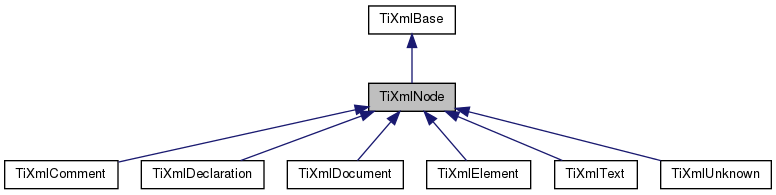
\includegraphics[width=350pt]{class_ti_xml_node__inherit__graph}
\end{center}
\end{figure}


\-Collaboration diagram for \-Ti\-Xml\-Node\-:
\nopagebreak
\begin{figure}[H]
\begin{center}
\leavevmode
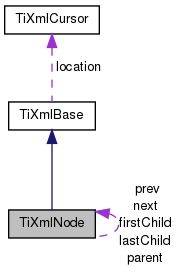
\includegraphics[width=205pt]{class_ti_xml_node__coll__graph}
\end{center}
\end{figure}
\subsection*{\-Public \-Types}
\begin{DoxyCompactItemize}
\item 
enum \hyperlink{class_ti_xml_node_a836eded4920ab9e9ef28496f48cd95a2}{\-Node\-Type} \{ \*
{\bfseries \-T\-I\-N\-Y\-X\-M\-L\-\_\-\-D\-O\-C\-U\-M\-E\-N\-T}, 
{\bfseries \-T\-I\-N\-Y\-X\-M\-L\-\_\-\-E\-L\-E\-M\-E\-N\-T}, 
{\bfseries \-T\-I\-N\-Y\-X\-M\-L\-\_\-\-C\-O\-M\-M\-E\-N\-T}, 
{\bfseries \-T\-I\-N\-Y\-X\-M\-L\-\_\-\-U\-N\-K\-N\-O\-W\-N}, 
\*
{\bfseries \-T\-I\-N\-Y\-X\-M\-L\-\_\-\-T\-E\-X\-T}, 
{\bfseries \-T\-I\-N\-Y\-X\-M\-L\-\_\-\-D\-E\-C\-L\-A\-R\-A\-T\-I\-O\-N}, 
{\bfseries \-T\-I\-N\-Y\-X\-M\-L\-\_\-\-T\-Y\-P\-E\-C\-O\-U\-N\-T}
 \}
\end{DoxyCompactItemize}
\subsection*{\-Public \-Member \-Functions}
\begin{DoxyCompactItemize}
\item 
const char $\ast$ \hyperlink{class_ti_xml_node_a77943eb90d12c2892b1337a9f5918b41}{\-Value} () const 
\item 
\hypertarget{class_ti_xml_node_a83ece13d2ea66dac66e0b21332229239}{const \-T\-I\-X\-M\-L\-\_\-\-S\-T\-R\-I\-N\-G \& {\bfseries \-Value\-T\-Str} () const }\label{class_ti_xml_node_a83ece13d2ea66dac66e0b21332229239}

\item 
void \hyperlink{class_ti_xml_node_a2a38329ca5d3f28f98ce932b8299ae90}{\-Set\-Value} (const char $\ast$\-\_\-value)
\item 
\hypertarget{class_ti_xml_node_a708e7f953df61d4d2d12f73171550a4b}{void \hyperlink{class_ti_xml_node_a708e7f953df61d4d2d12f73171550a4b}{\-Clear} ()}\label{class_ti_xml_node_a708e7f953df61d4d2d12f73171550a4b}

\begin{DoxyCompactList}\small\item\em \-Delete all the children of this node. \-Does not affect 'this'. \end{DoxyCompactList}\item 
\hypertarget{class_ti_xml_node_ab643043132ffd794f8602685d34a982e}{\hyperlink{class_ti_xml_node}{\-Ti\-Xml\-Node} $\ast$ \hyperlink{class_ti_xml_node_ab643043132ffd794f8602685d34a982e}{\-Parent} ()}\label{class_ti_xml_node_ab643043132ffd794f8602685d34a982e}

\begin{DoxyCompactList}\small\item\em \-One step up the \-D\-O\-M. \end{DoxyCompactList}\item 
\hypertarget{class_ti_xml_node_a78878709e53066f06eb4fcbcdd3a5260}{const \hyperlink{class_ti_xml_node}{\-Ti\-Xml\-Node} $\ast$ {\bfseries \-Parent} () const }\label{class_ti_xml_node_a78878709e53066f06eb4fcbcdd3a5260}

\item 
\hypertarget{class_ti_xml_node_a44c8eee26bbe2d1b2762038df9dde2f0}{const \hyperlink{class_ti_xml_node}{\-Ti\-Xml\-Node} $\ast$ \hyperlink{class_ti_xml_node_a44c8eee26bbe2d1b2762038df9dde2f0}{\-First\-Child} () const }\label{class_ti_xml_node_a44c8eee26bbe2d1b2762038df9dde2f0}

\begin{DoxyCompactList}\small\item\em \-The first child of this node. \-Will be null if there are no children. \end{DoxyCompactList}\item 
\hypertarget{class_ti_xml_node_a5e97d69b7c0ebd27fb7286be56559b77}{\hyperlink{class_ti_xml_node}{\-Ti\-Xml\-Node} $\ast$ {\bfseries \-First\-Child} ()}\label{class_ti_xml_node_a5e97d69b7c0ebd27fb7286be56559b77}

\item 
const \hyperlink{class_ti_xml_node}{\-Ti\-Xml\-Node} $\ast$ \hyperlink{class_ti_xml_node_ab5f722624113c8203227de4f56576d31}{\-First\-Child} (const char $\ast$value) const 
\item 
\hypertarget{class_ti_xml_node_abc8bf32be6419ec453a731868de19554}{\hyperlink{class_ti_xml_node}{\-Ti\-Xml\-Node} $\ast$ \hyperlink{class_ti_xml_node_abc8bf32be6419ec453a731868de19554}{\-First\-Child} (const char $\ast$\-\_\-value)}\label{class_ti_xml_node_abc8bf32be6419ec453a731868de19554}

\begin{DoxyCompactList}\small\item\em \-The first child of this node with the matching 'value'. \-Will be null if none found. \end{DoxyCompactList}\item 
\hypertarget{class_ti_xml_node_a6d671107e00cca1d28cb2d7f3a87a21e}{const \hyperlink{class_ti_xml_node}{\-Ti\-Xml\-Node} $\ast$ {\bfseries \-Last\-Child} () const }\label{class_ti_xml_node_a6d671107e00cca1d28cb2d7f3a87a21e}

\item 
\hypertarget{class_ti_xml_node_a6432d2b2495f6caf9cb4278df706a031}{\hyperlink{class_ti_xml_node}{\-Ti\-Xml\-Node} $\ast$ \hyperlink{class_ti_xml_node_a6432d2b2495f6caf9cb4278df706a031}{\-Last\-Child} ()}\label{class_ti_xml_node_a6432d2b2495f6caf9cb4278df706a031}

\begin{DoxyCompactList}\small\item\em \-The last child of this node. \-Will be null if there are no children. \end{DoxyCompactList}\item 
\hypertarget{class_ti_xml_node_acdd3fdc436aa7433023310a041e5e63f}{const \hyperlink{class_ti_xml_node}{\-Ti\-Xml\-Node} $\ast$ {\bfseries \-Last\-Child} (const char $\ast$value) const }\label{class_ti_xml_node_acdd3fdc436aa7433023310a041e5e63f}

\item 
\hypertarget{class_ti_xml_node_abad5bf1059c48127b958711ef89e8e5d}{\hyperlink{class_ti_xml_node}{\-Ti\-Xml\-Node} $\ast$ \hyperlink{class_ti_xml_node_abad5bf1059c48127b958711ef89e8e5d}{\-Last\-Child} (const char $\ast$\-\_\-value)}\label{class_ti_xml_node_abad5bf1059c48127b958711ef89e8e5d}

\begin{DoxyCompactList}\small\item\em \-The last child of this node matching 'value'. \-Will be null if there are no children. \end{DoxyCompactList}\item 
const \hyperlink{class_ti_xml_node}{\-Ti\-Xml\-Node} $\ast$ \hyperlink{class_ti_xml_node_aaef7ac3978c4bb1cc8a24ffae7bced75}{\-Iterate\-Children} (const \hyperlink{class_ti_xml_node}{\-Ti\-Xml\-Node} $\ast$previous) const 
\item 
\hypertarget{class_ti_xml_node_a2358e747118fdbf0e467b1e4f7d03de1}{\hyperlink{class_ti_xml_node}{\-Ti\-Xml\-Node} $\ast$ {\bfseries \-Iterate\-Children} (const \hyperlink{class_ti_xml_node}{\-Ti\-Xml\-Node} $\ast$previous)}\label{class_ti_xml_node_a2358e747118fdbf0e467b1e4f7d03de1}

\item 
\hypertarget{class_ti_xml_node_af2b86dbe25d3d26fa48180edc5e2a9fc}{const \hyperlink{class_ti_xml_node}{\-Ti\-Xml\-Node} $\ast$ \hyperlink{class_ti_xml_node_af2b86dbe25d3d26fa48180edc5e2a9fc}{\-Iterate\-Children} (const char $\ast$value, const \hyperlink{class_ti_xml_node}{\-Ti\-Xml\-Node} $\ast$previous) const }\label{class_ti_xml_node_af2b86dbe25d3d26fa48180edc5e2a9fc}

\begin{DoxyCompactList}\small\item\em \-This flavor of \-Iterate\-Children searches for children with a particular 'value'. \end{DoxyCompactList}\item 
\hypertarget{class_ti_xml_node_a67ba8275e533e6f76340236c42ea0aea}{\hyperlink{class_ti_xml_node}{\-Ti\-Xml\-Node} $\ast$ {\bfseries \-Iterate\-Children} (const char $\ast$\-\_\-value, const \hyperlink{class_ti_xml_node}{\-Ti\-Xml\-Node} $\ast$previous)}\label{class_ti_xml_node_a67ba8275e533e6f76340236c42ea0aea}

\item 
\hyperlink{class_ti_xml_node}{\-Ti\-Xml\-Node} $\ast$ \hyperlink{class_ti_xml_node_af287a913ce46d8dbf7ef24fec69bbaf0}{\-Insert\-End\-Child} (const \hyperlink{class_ti_xml_node}{\-Ti\-Xml\-Node} \&add\-This)
\item 
\hyperlink{class_ti_xml_node}{\-Ti\-Xml\-Node} $\ast$ \hyperlink{class_ti_xml_node_a1a881212554b759865f6cac79a851d38}{\-Link\-End\-Child} (\hyperlink{class_ti_xml_node}{\-Ti\-Xml\-Node} $\ast$add\-This)
\item 
\hyperlink{class_ti_xml_node}{\-Ti\-Xml\-Node} $\ast$ \hyperlink{class_ti_xml_node_a71e54e393336382bc9875f64aab5cb15}{\-Insert\-Before\-Child} (\hyperlink{class_ti_xml_node}{\-Ti\-Xml\-Node} $\ast$before\-This, const \hyperlink{class_ti_xml_node}{\-Ti\-Xml\-Node} \&add\-This)
\item 
\hyperlink{class_ti_xml_node}{\-Ti\-Xml\-Node} $\ast$ \hyperlink{class_ti_xml_node_a274db3292218202805c093f66a964cb5}{\-Insert\-After\-Child} (\hyperlink{class_ti_xml_node}{\-Ti\-Xml\-Node} $\ast$after\-This, const \hyperlink{class_ti_xml_node}{\-Ti\-Xml\-Node} \&add\-This)
\item 
\hyperlink{class_ti_xml_node}{\-Ti\-Xml\-Node} $\ast$ \hyperlink{class_ti_xml_node_a543208c2c801c84a213529541e904b9f}{\-Replace\-Child} (\hyperlink{class_ti_xml_node}{\-Ti\-Xml\-Node} $\ast$replace\-This, const \hyperlink{class_ti_xml_node}{\-Ti\-Xml\-Node} \&with\-This)
\item 
\hypertarget{class_ti_xml_node_ae19d8510efc90596552f4feeac9a8fbf}{bool \hyperlink{class_ti_xml_node_ae19d8510efc90596552f4feeac9a8fbf}{\-Remove\-Child} (\hyperlink{class_ti_xml_node}{\-Ti\-Xml\-Node} $\ast$remove\-This)}\label{class_ti_xml_node_ae19d8510efc90596552f4feeac9a8fbf}

\begin{DoxyCompactList}\small\item\em \-Delete a child of this node. \end{DoxyCompactList}\item 
\hypertarget{class_ti_xml_node_ac2cd892768726270e511b2ab32de4d10}{const \hyperlink{class_ti_xml_node}{\-Ti\-Xml\-Node} $\ast$ \hyperlink{class_ti_xml_node_ac2cd892768726270e511b2ab32de4d10}{\-Previous\-Sibling} () const }\label{class_ti_xml_node_ac2cd892768726270e511b2ab32de4d10}

\begin{DoxyCompactList}\small\item\em \-Navigate to a sibling node. \end{DoxyCompactList}\item 
\hypertarget{class_ti_xml_node_af8c0642ad6ecc03f62953e68896ed1cc}{\hyperlink{class_ti_xml_node}{\-Ti\-Xml\-Node} $\ast$ {\bfseries \-Previous\-Sibling} ()}\label{class_ti_xml_node_af8c0642ad6ecc03f62953e68896ed1cc}

\item 
\hypertarget{class_ti_xml_node_abbb3b8c1f38fa7b9e52d584a4aeca795}{const \hyperlink{class_ti_xml_node}{\-Ti\-Xml\-Node} $\ast$ \hyperlink{class_ti_xml_node_abbb3b8c1f38fa7b9e52d584a4aeca795}{\-Previous\-Sibling} (const char $\ast$) const }\label{class_ti_xml_node_abbb3b8c1f38fa7b9e52d584a4aeca795}

\begin{DoxyCompactList}\small\item\em \-Navigate to a sibling node. \end{DoxyCompactList}\item 
\hypertarget{class_ti_xml_node_a6c977049207177ef21b51972315c2053}{\hyperlink{class_ti_xml_node}{\-Ti\-Xml\-Node} $\ast$ {\bfseries \-Previous\-Sibling} (const char $\ast$\-\_\-prev)}\label{class_ti_xml_node_a6c977049207177ef21b51972315c2053}

\item 
\hypertarget{class_ti_xml_node_af854baeba384f5fe9859f5aee03b548e}{const \hyperlink{class_ti_xml_node}{\-Ti\-Xml\-Node} $\ast$ \hyperlink{class_ti_xml_node_af854baeba384f5fe9859f5aee03b548e}{\-Next\-Sibling} () const }\label{class_ti_xml_node_af854baeba384f5fe9859f5aee03b548e}

\begin{DoxyCompactList}\small\item\em \-Navigate to a sibling node. \end{DoxyCompactList}\item 
\hypertarget{class_ti_xml_node_a4d05f7b1d7b470ac6887edd072d4892a}{\hyperlink{class_ti_xml_node}{\-Ti\-Xml\-Node} $\ast$ {\bfseries \-Next\-Sibling} ()}\label{class_ti_xml_node_a4d05f7b1d7b470ac6887edd072d4892a}

\item 
\hypertarget{class_ti_xml_node_acaf9dc17531ac041f602f9ad579573ea}{const \hyperlink{class_ti_xml_node}{\-Ti\-Xml\-Node} $\ast$ \hyperlink{class_ti_xml_node_acaf9dc17531ac041f602f9ad579573ea}{\-Next\-Sibling} (const char $\ast$) const }\label{class_ti_xml_node_acaf9dc17531ac041f602f9ad579573ea}

\begin{DoxyCompactList}\small\item\em \-Navigate to a sibling node with the given 'value'. \end{DoxyCompactList}\item 
\hypertarget{class_ti_xml_node_a4080bc5cc8a5c139e7cf308669e850fc}{\hyperlink{class_ti_xml_node}{\-Ti\-Xml\-Node} $\ast$ {\bfseries \-Next\-Sibling} (const char $\ast$\-\_\-next)}\label{class_ti_xml_node_a4080bc5cc8a5c139e7cf308669e850fc}

\item 
const \hyperlink{class_ti_xml_element}{\-Ti\-Xml\-Element} $\ast$ \hyperlink{class_ti_xml_node_a7667217e269e0da01d1f82aee94d1a3d}{\-Next\-Sibling\-Element} () const 
\item 
\hypertarget{class_ti_xml_node_a1b211cb5034655a04358e0e2f6fc5010}{\hyperlink{class_ti_xml_element}{\-Ti\-Xml\-Element} $\ast$ {\bfseries \-Next\-Sibling\-Element} ()}\label{class_ti_xml_node_a1b211cb5034655a04358e0e2f6fc5010}

\item 
const \hyperlink{class_ti_xml_element}{\-Ti\-Xml\-Element} $\ast$ \hyperlink{class_ti_xml_node_a3d7897999f99cf4870dd59df6331d7ff}{\-Next\-Sibling\-Element} (const char $\ast$) const 
\item 
\hypertarget{class_ti_xml_node_a6e1ac6b800e18049bc75e9f8e63a8e5f}{\hyperlink{class_ti_xml_element}{\-Ti\-Xml\-Element} $\ast$ {\bfseries \-Next\-Sibling\-Element} (const char $\ast$\-\_\-next)}\label{class_ti_xml_node_a6e1ac6b800e18049bc75e9f8e63a8e5f}

\item 
\hypertarget{class_ti_xml_node_ab1f8d8e70d88aea4c5efedfe00862d55}{const \hyperlink{class_ti_xml_element}{\-Ti\-Xml\-Element} $\ast$ \hyperlink{class_ti_xml_node_ab1f8d8e70d88aea4c5efedfe00862d55}{\-First\-Child\-Element} () const }\label{class_ti_xml_node_ab1f8d8e70d88aea4c5efedfe00862d55}

\begin{DoxyCompactList}\small\item\em \-Convenience function to get through elements. \end{DoxyCompactList}\item 
\hypertarget{class_ti_xml_node_aa0fecff1f3866ab33a8a25506e95db1d}{\hyperlink{class_ti_xml_element}{\-Ti\-Xml\-Element} $\ast$ {\bfseries \-First\-Child\-Element} ()}\label{class_ti_xml_node_aa0fecff1f3866ab33a8a25506e95db1d}

\item 
\hypertarget{class_ti_xml_node_a0ec361bfef1cf1978d060295f597e0d9}{const \hyperlink{class_ti_xml_element}{\-Ti\-Xml\-Element} $\ast$ \hyperlink{class_ti_xml_node_a0ec361bfef1cf1978d060295f597e0d9}{\-First\-Child\-Element} (const char $\ast$\-\_\-value) const }\label{class_ti_xml_node_a0ec361bfef1cf1978d060295f597e0d9}

\begin{DoxyCompactList}\small\item\em \-Convenience function to get through elements. \end{DoxyCompactList}\item 
\hypertarget{class_ti_xml_node_a6936ae323675071808ac4840379e57f5}{\hyperlink{class_ti_xml_element}{\-Ti\-Xml\-Element} $\ast$ {\bfseries \-First\-Child\-Element} (const char $\ast$\-\_\-value)}\label{class_ti_xml_node_a6936ae323675071808ac4840379e57f5}

\item 
int \hyperlink{class_ti_xml_node_a57b99d5c97d67a42b9752f5210a1ba5e}{\-Type} () const 
\item 
const \hyperlink{class_ti_xml_document}{\-Ti\-Xml\-Document} $\ast$ \hyperlink{class_ti_xml_node_aa66f4ebcd175204a168ed7c2d7b43071}{\-Get\-Document} () const 
\item 
\hypertarget{class_ti_xml_node_a7b2372c0e7adfb32f5b6902fe49a39b2}{\hyperlink{class_ti_xml_document}{\-Ti\-Xml\-Document} $\ast$ {\bfseries \-Get\-Document} ()}\label{class_ti_xml_node_a7b2372c0e7adfb32f5b6902fe49a39b2}

\item 
\hypertarget{class_ti_xml_node_aeed21ad30630ef6e7faf096127edc9f3}{bool \hyperlink{class_ti_xml_node_aeed21ad30630ef6e7faf096127edc9f3}{\-No\-Children} () const }\label{class_ti_xml_node_aeed21ad30630ef6e7faf096127edc9f3}

\begin{DoxyCompactList}\small\item\em \-Returns true if this node has no children. \end{DoxyCompactList}\item 
\hypertarget{class_ti_xml_node_a8a4cda4b15c29f64cff419309aebed08}{virtual const \hyperlink{class_ti_xml_document}{\-Ti\-Xml\-Document} $\ast$ \hyperlink{class_ti_xml_node_a8a4cda4b15c29f64cff419309aebed08}{\-To\-Document} () const }\label{class_ti_xml_node_a8a4cda4b15c29f64cff419309aebed08}

\begin{DoxyCompactList}\small\item\em \-Cast to a more defined type. \-Will return null if not of the requested type. \end{DoxyCompactList}\item 
\hypertarget{class_ti_xml_node_a72abed96dc9667ab9e0a2a275301bb1c}{virtual const \hyperlink{class_ti_xml_element}{\-Ti\-Xml\-Element} $\ast$ \hyperlink{class_ti_xml_node_a72abed96dc9667ab9e0a2a275301bb1c}{\-To\-Element} () const }\label{class_ti_xml_node_a72abed96dc9667ab9e0a2a275301bb1c}

\begin{DoxyCompactList}\small\item\em \-Cast to a more defined type. \-Will return null if not of the requested type. \end{DoxyCompactList}\item 
\hypertarget{class_ti_xml_node_aa0a5086f9eaee910bbfdc7f975e26574}{virtual const \hyperlink{class_ti_xml_comment}{\-Ti\-Xml\-Comment} $\ast$ \hyperlink{class_ti_xml_node_aa0a5086f9eaee910bbfdc7f975e26574}{\-To\-Comment} () const }\label{class_ti_xml_node_aa0a5086f9eaee910bbfdc7f975e26574}

\begin{DoxyCompactList}\small\item\em \-Cast to a more defined type. \-Will return null if not of the requested type. \end{DoxyCompactList}\item 
\hypertarget{class_ti_xml_node_afd7205cf31d7a376929f8a36930627a2}{virtual const \hyperlink{class_ti_xml_unknown}{\-Ti\-Xml\-Unknown} $\ast$ \hyperlink{class_ti_xml_node_afd7205cf31d7a376929f8a36930627a2}{\-To\-Unknown} () const }\label{class_ti_xml_node_afd7205cf31d7a376929f8a36930627a2}

\begin{DoxyCompactList}\small\item\em \-Cast to a more defined type. \-Will return null if not of the requested type. \end{DoxyCompactList}\item 
\hypertarget{class_ti_xml_node_a95a46a52c525992d6b4ee08beb14cd69}{virtual const \hyperlink{class_ti_xml_text}{\-Ti\-Xml\-Text} $\ast$ \hyperlink{class_ti_xml_node_a95a46a52c525992d6b4ee08beb14cd69}{\-To\-Text} () const }\label{class_ti_xml_node_a95a46a52c525992d6b4ee08beb14cd69}

\begin{DoxyCompactList}\small\item\em \-Cast to a more defined type. \-Will return null if not of the requested type. \end{DoxyCompactList}\item 
\hypertarget{class_ti_xml_node_a9f43e6984fc7d4afd6eb32714c6b7b72}{virtual const \hyperlink{class_ti_xml_declaration}{\-Ti\-Xml\-Declaration} $\ast$ \hyperlink{class_ti_xml_node_a9f43e6984fc7d4afd6eb32714c6b7b72}{\-To\-Declaration} () const }\label{class_ti_xml_node_a9f43e6984fc7d4afd6eb32714c6b7b72}

\begin{DoxyCompactList}\small\item\em \-Cast to a more defined type. \-Will return null if not of the requested type. \end{DoxyCompactList}\item 
\hypertarget{class_ti_xml_node_a6a4c8ac28ee7a745d059db6691e03bae}{virtual \hyperlink{class_ti_xml_document}{\-Ti\-Xml\-Document} $\ast$ \hyperlink{class_ti_xml_node_a6a4c8ac28ee7a745d059db6691e03bae}{\-To\-Document} ()}\label{class_ti_xml_node_a6a4c8ac28ee7a745d059db6691e03bae}

\begin{DoxyCompactList}\small\item\em \-Cast to a more defined type. \-Will return null if not of the requested type. \end{DoxyCompactList}\item 
\hypertarget{class_ti_xml_node_aa65d000223187d22a4dcebd7479e9ebc}{virtual \hyperlink{class_ti_xml_element}{\-Ti\-Xml\-Element} $\ast$ \hyperlink{class_ti_xml_node_aa65d000223187d22a4dcebd7479e9ebc}{\-To\-Element} ()}\label{class_ti_xml_node_aa65d000223187d22a4dcebd7479e9ebc}

\begin{DoxyCompactList}\small\item\em \-Cast to a more defined type. \-Will return null if not of the requested type. \end{DoxyCompactList}\item 
\hypertarget{class_ti_xml_node_a383e06a0787f7063953934867990f849}{virtual \hyperlink{class_ti_xml_comment}{\-Ti\-Xml\-Comment} $\ast$ \hyperlink{class_ti_xml_node_a383e06a0787f7063953934867990f849}{\-To\-Comment} ()}\label{class_ti_xml_node_a383e06a0787f7063953934867990f849}

\begin{DoxyCompactList}\small\item\em \-Cast to a more defined type. \-Will return null if not of the requested type. \end{DoxyCompactList}\item 
\hypertarget{class_ti_xml_node_a06de5af852668c7e4af0d09c205f0b0d}{virtual \hyperlink{class_ti_xml_unknown}{\-Ti\-Xml\-Unknown} $\ast$ \hyperlink{class_ti_xml_node_a06de5af852668c7e4af0d09c205f0b0d}{\-To\-Unknown} ()}\label{class_ti_xml_node_a06de5af852668c7e4af0d09c205f0b0d}

\begin{DoxyCompactList}\small\item\em \-Cast to a more defined type. \-Will return null if not of the requested type. \end{DoxyCompactList}\item 
\hypertarget{class_ti_xml_node_a3ddfbcac78fbea041fad57e5c6d60a03}{virtual \hyperlink{class_ti_xml_text}{\-Ti\-Xml\-Text} $\ast$ \hyperlink{class_ti_xml_node_a3ddfbcac78fbea041fad57e5c6d60a03}{\-To\-Text} ()}\label{class_ti_xml_node_a3ddfbcac78fbea041fad57e5c6d60a03}

\begin{DoxyCompactList}\small\item\em \-Cast to a more defined type. \-Will return null if not of the requested type. \end{DoxyCompactList}\item 
\hypertarget{class_ti_xml_node_a4027136ca820ff4a636b607231b6a6df}{virtual \hyperlink{class_ti_xml_declaration}{\-Ti\-Xml\-Declaration} $\ast$ \hyperlink{class_ti_xml_node_a4027136ca820ff4a636b607231b6a6df}{\-To\-Declaration} ()}\label{class_ti_xml_node_a4027136ca820ff4a636b607231b6a6df}

\begin{DoxyCompactList}\small\item\em \-Cast to a more defined type. \-Will return null if not of the requested type. \end{DoxyCompactList}\item 
virtual \hyperlink{class_ti_xml_node}{\-Ti\-Xml\-Node} $\ast$ \hyperlink{class_ti_xml_node_a4508cc3a2d7a98e96a54cc09c37a78a4}{\-Clone} () const =0
\item 
virtual bool \hyperlink{class_ti_xml_node_acc0f88b7462c6cb73809d410a4f5bb86}{\-Accept} (\hyperlink{class_ti_xml_visitor}{\-Ti\-Xml\-Visitor} $\ast$visitor) const =0
\end{DoxyCompactItemize}
\subsection*{\-Protected \-Member \-Functions}
\begin{DoxyCompactItemize}
\item 
\hypertarget{class_ti_xml_node_a3f46721695868667113c7487ff123f20}{{\bfseries \-Ti\-Xml\-Node} (\hyperlink{class_ti_xml_node_a836eded4920ab9e9ef28496f48cd95a2}{\-Node\-Type} \-\_\-type)}\label{class_ti_xml_node_a3f46721695868667113c7487ff123f20}

\item 
\hypertarget{class_ti_xml_node_ab6056978923ad8350fb5164af32d8038}{void {\bfseries \-Copy\-To} (\hyperlink{class_ti_xml_node}{\-Ti\-Xml\-Node} $\ast$target) const }\label{class_ti_xml_node_ab6056978923ad8350fb5164af32d8038}

\item 
\hypertarget{class_ti_xml_node_ac1e3a8e7578be463b04617786120c2bb}{\hyperlink{class_ti_xml_node}{\-Ti\-Xml\-Node} $\ast$ {\bfseries \-Identify} (const char $\ast$start, \-Ti\-Xml\-Encoding encoding)}\label{class_ti_xml_node_ac1e3a8e7578be463b04617786120c2bb}

\end{DoxyCompactItemize}
\subsection*{\-Protected \-Attributes}
\begin{DoxyCompactItemize}
\item 
\hypertarget{class_ti_xml_node_a662c4de61244e4fa5bd4e2d8c63143a5}{\hyperlink{class_ti_xml_node}{\-Ti\-Xml\-Node} $\ast$ {\bfseries parent}}\label{class_ti_xml_node_a662c4de61244e4fa5bd4e2d8c63143a5}

\item 
\hypertarget{class_ti_xml_node_a2619c6379181c16ba95ae6922e2ca839}{\hyperlink{class_ti_xml_node_a836eded4920ab9e9ef28496f48cd95a2}{\-Node\-Type} {\bfseries type}}\label{class_ti_xml_node_a2619c6379181c16ba95ae6922e2ca839}

\item 
\hypertarget{class_ti_xml_node_af749fb7f22010b80e8f904c32653d50e}{\hyperlink{class_ti_xml_node}{\-Ti\-Xml\-Node} $\ast$ {\bfseries first\-Child}}\label{class_ti_xml_node_af749fb7f22010b80e8f904c32653d50e}

\item 
\hypertarget{class_ti_xml_node_a5b30756d21b304580d22a841ec9d61f8}{\hyperlink{class_ti_xml_node}{\-Ti\-Xml\-Node} $\ast$ {\bfseries last\-Child}}\label{class_ti_xml_node_a5b30756d21b304580d22a841ec9d61f8}

\item 
\hypertarget{class_ti_xml_node_aead528b3cedc33c16a6c539872c7cc8b}{\-T\-I\-X\-M\-L\-\_\-\-S\-T\-R\-I\-N\-G {\bfseries value}}\label{class_ti_xml_node_aead528b3cedc33c16a6c539872c7cc8b}

\item 
\hypertarget{class_ti_xml_node_a9c5370ea2cbfd9f0e0f7b30a57fd68f5}{\hyperlink{class_ti_xml_node}{\-Ti\-Xml\-Node} $\ast$ {\bfseries prev}}\label{class_ti_xml_node_a9c5370ea2cbfd9f0e0f7b30a57fd68f5}

\item 
\hypertarget{class_ti_xml_node_a2f329cc993d2d34df76e17dcbb776b45}{\hyperlink{class_ti_xml_node}{\-Ti\-Xml\-Node} $\ast$ {\bfseries next}}\label{class_ti_xml_node_a2f329cc993d2d34df76e17dcbb776b45}

\end{DoxyCompactItemize}
\subsection*{\-Friends}
\begin{DoxyCompactItemize}
\item 
\hypertarget{class_ti_xml_node_a173617f6dfe902cf484ce5552b950475}{class {\bfseries \-Ti\-Xml\-Document}}\label{class_ti_xml_node_a173617f6dfe902cf484ce5552b950475}

\item 
\hypertarget{class_ti_xml_node_ab6592e32cb9132be517cc12a70564c4b}{class {\bfseries \-Ti\-Xml\-Element}}\label{class_ti_xml_node_ab6592e32cb9132be517cc12a70564c4b}

\end{DoxyCompactItemize}


\subsection{\-Detailed \-Description}
\-The parent class for everything in the \-Document \-Object \-Model. (\-Except for attributes). \-Nodes have siblings, a parent, and children. \-A node can be in a document, or stand on its own. \-The type of a \hyperlink{class_ti_xml_node}{\-Ti\-Xml\-Node} can be queried, and it can be cast to its more defined type. 

\subsection{\-Member \-Enumeration \-Documentation}
\hypertarget{class_ti_xml_node_a836eded4920ab9e9ef28496f48cd95a2}{\index{\-Ti\-Xml\-Node@{\-Ti\-Xml\-Node}!\-Node\-Type@{\-Node\-Type}}
\index{\-Node\-Type@{\-Node\-Type}!TiXmlNode@{\-Ti\-Xml\-Node}}
\subsubsection[{\-Node\-Type}]{\setlength{\rightskip}{0pt plus 5cm}enum {\bf \-Ti\-Xml\-Node\-::\-Node\-Type}}}\label{class_ti_xml_node_a836eded4920ab9e9ef28496f48cd95a2}
\-The types of \-X\-M\-L nodes supported by \-Tiny\-Xml. (\-All the unsupported types are picked up by \-U\-N\-K\-N\-O\-W\-N.) 

\subsection{\-Member \-Function \-Documentation}
\hypertarget{class_ti_xml_node_acc0f88b7462c6cb73809d410a4f5bb86}{\index{\-Ti\-Xml\-Node@{\-Ti\-Xml\-Node}!\-Accept@{\-Accept}}
\index{\-Accept@{\-Accept}!TiXmlNode@{\-Ti\-Xml\-Node}}
\subsubsection[{\-Accept}]{\setlength{\rightskip}{0pt plus 5cm}virtual bool {\bf \-Ti\-Xml\-Node\-::\-Accept} (
\begin{DoxyParamCaption}
\item[{{\bf \-Ti\-Xml\-Visitor} $\ast$}]{visitor}
\end{DoxyParamCaption}
) const\hspace{0.3cm}{\ttfamily  \mbox{[}pure virtual\mbox{]}}}}\label{class_ti_xml_node_acc0f88b7462c6cb73809d410a4f5bb86}
\-Accept a hierchical visit the nodes in the \-Tiny\-X\-M\-L \-D\-O\-M. \-Every node in the \-X\-M\-L tree will be conditionally visited and the host will be called back via the \hyperlink{class_ti_xml_visitor}{\-Ti\-Xml\-Visitor} interface.

\-This is essentially a \-S\-A\-X interface for \-Tiny\-X\-M\-L. (\-Note however it doesn't re-\/parse the \-X\-M\-L for the callbacks, so the performance of \-Tiny\-X\-M\-L is unchanged by using this interface versus any other.)

\-The interface has been based on ideas from\-:


\begin{DoxyItemize}
\item \href{http://www.saxproject.org/}{\tt http\-://www.\-saxproject.\-org/}
\item \href{http://c2.com/cgi/wiki?HierarchicalVisitorPattern}{\tt http\-://c2.\-com/cgi/wiki?\-Hierarchical\-Visitor\-Pattern}
\end{DoxyItemize}

\-Which are both good references for \char`\"{}visiting\char`\"{}.

\-An example of using \hyperlink{class_ti_xml_node_acc0f88b7462c6cb73809d410a4f5bb86}{\-Accept()}\-: \begin{DoxyVerb}
		TiXmlPrinter printer;
		tinyxmlDoc.Accept( &printer );
		const char* xmlcstr = printer.CStr();
		\end{DoxyVerb}
 

\-Implemented in \hyperlink{class_ti_xml_document_a3daab2f472418ef66315750202f762ae}{\-Ti\-Xml\-Document}, \hyperlink{class_ti_xml_unknown_a4e54d7482e05a837cf83c925cc683380}{\-Ti\-Xml\-Unknown}, \hyperlink{class_ti_xml_declaration_ab6a6b178161ba9abc2c35058de689864}{\-Ti\-Xml\-Declaration}, \hyperlink{class_ti_xml_text_a43b9954ebf679557fac1a4453f337b7c}{\-Ti\-Xml\-Text}, \hyperlink{class_ti_xml_comment_a4382de0e50da973f11a23ea5852568bd}{\-Ti\-Xml\-Comment}, and \hyperlink{class_ti_xml_element_a31ab28cc3b892a69254391d6bbe08df3}{\-Ti\-Xml\-Element}.

\hypertarget{class_ti_xml_node_a4508cc3a2d7a98e96a54cc09c37a78a4}{\index{\-Ti\-Xml\-Node@{\-Ti\-Xml\-Node}!\-Clone@{\-Clone}}
\index{\-Clone@{\-Clone}!TiXmlNode@{\-Ti\-Xml\-Node}}
\subsubsection[{\-Clone}]{\setlength{\rightskip}{0pt plus 5cm}virtual {\bf \-Ti\-Xml\-Node}$\ast$ {\bf \-Ti\-Xml\-Node\-::\-Clone} (
\begin{DoxyParamCaption}
{}
\end{DoxyParamCaption}
) const\hspace{0.3cm}{\ttfamily  \mbox{[}pure virtual\mbox{]}}}}\label{class_ti_xml_node_a4508cc3a2d7a98e96a54cc09c37a78a4}
\-Create an exact duplicate of this node and return it. \-The memory must be deleted by the caller. 

\-Implemented in \hyperlink{class_ti_xml_document_ac9e8f09b23454d953b32d1b65cd1409e}{\-Ti\-Xml\-Document}, \hyperlink{class_ti_xml_unknown_a675c4b2684af35e4c7649b7fd5ae598d}{\-Ti\-Xml\-Unknown}, \hyperlink{class_ti_xml_declaration_aff8231266d735943d8a7514a9c9822b9}{\-Ti\-Xml\-Declaration}, \hyperlink{class_ti_xml_text_adde1869dfb029be50713fbfd8ce4d21f}{\-Ti\-Xml\-Text}, \hyperlink{class_ti_xml_comment_a4f6590c9c9a2b63a48972655b78eb853}{\-Ti\-Xml\-Comment}, and \hyperlink{class_ti_xml_element_a13f6df105ebb1e8dc636e75cc883be32}{\-Ti\-Xml\-Element}.

\hypertarget{class_ti_xml_node_ab5f722624113c8203227de4f56576d31}{\index{\-Ti\-Xml\-Node@{\-Ti\-Xml\-Node}!\-First\-Child@{\-First\-Child}}
\index{\-First\-Child@{\-First\-Child}!TiXmlNode@{\-Ti\-Xml\-Node}}
\subsubsection[{\-First\-Child}]{\setlength{\rightskip}{0pt plus 5cm}const {\bf \-Ti\-Xml\-Node} $\ast$ {\bf \-Ti\-Xml\-Node\-::\-First\-Child} (
\begin{DoxyParamCaption}
\item[{const char $\ast$}]{value}
\end{DoxyParamCaption}
) const}}\label{class_ti_xml_node_ab5f722624113c8203227de4f56576d31}
\-The first child of this node with the matching 'value'. \-Will be null if none found. \hypertarget{class_ti_xml_node_aa66f4ebcd175204a168ed7c2d7b43071}{\index{\-Ti\-Xml\-Node@{\-Ti\-Xml\-Node}!\-Get\-Document@{\-Get\-Document}}
\index{\-Get\-Document@{\-Get\-Document}!TiXmlNode@{\-Ti\-Xml\-Node}}
\subsubsection[{\-Get\-Document}]{\setlength{\rightskip}{0pt plus 5cm}const {\bf \-Ti\-Xml\-Document} $\ast$ {\bf \-Ti\-Xml\-Node\-::\-Get\-Document} (
\begin{DoxyParamCaption}
{}
\end{DoxyParamCaption}
) const}}\label{class_ti_xml_node_aa66f4ebcd175204a168ed7c2d7b43071}
\-Return a pointer to the \-Document this node lives in. \-Returns null if not in a document. \hypertarget{class_ti_xml_node_a274db3292218202805c093f66a964cb5}{\index{\-Ti\-Xml\-Node@{\-Ti\-Xml\-Node}!\-Insert\-After\-Child@{\-Insert\-After\-Child}}
\index{\-Insert\-After\-Child@{\-Insert\-After\-Child}!TiXmlNode@{\-Ti\-Xml\-Node}}
\subsubsection[{\-Insert\-After\-Child}]{\setlength{\rightskip}{0pt plus 5cm}{\bf \-Ti\-Xml\-Node} $\ast$ {\bf \-Ti\-Xml\-Node\-::\-Insert\-After\-Child} (
\begin{DoxyParamCaption}
\item[{{\bf \-Ti\-Xml\-Node} $\ast$}]{after\-This, }
\item[{const {\bf \-Ti\-Xml\-Node} \&}]{add\-This}
\end{DoxyParamCaption}
)}}\label{class_ti_xml_node_a274db3292218202805c093f66a964cb5}
\-Add a new node related to this. \-Adds a child after the specified child. \-Returns a pointer to the new object or \-N\-U\-L\-L if an error occured. \hypertarget{class_ti_xml_node_a71e54e393336382bc9875f64aab5cb15}{\index{\-Ti\-Xml\-Node@{\-Ti\-Xml\-Node}!\-Insert\-Before\-Child@{\-Insert\-Before\-Child}}
\index{\-Insert\-Before\-Child@{\-Insert\-Before\-Child}!TiXmlNode@{\-Ti\-Xml\-Node}}
\subsubsection[{\-Insert\-Before\-Child}]{\setlength{\rightskip}{0pt plus 5cm}{\bf \-Ti\-Xml\-Node} $\ast$ {\bf \-Ti\-Xml\-Node\-::\-Insert\-Before\-Child} (
\begin{DoxyParamCaption}
\item[{{\bf \-Ti\-Xml\-Node} $\ast$}]{before\-This, }
\item[{const {\bf \-Ti\-Xml\-Node} \&}]{add\-This}
\end{DoxyParamCaption}
)}}\label{class_ti_xml_node_a71e54e393336382bc9875f64aab5cb15}
\-Add a new node related to this. \-Adds a child before the specified child. \-Returns a pointer to the new object or \-N\-U\-L\-L if an error occured. \hypertarget{class_ti_xml_node_af287a913ce46d8dbf7ef24fec69bbaf0}{\index{\-Ti\-Xml\-Node@{\-Ti\-Xml\-Node}!\-Insert\-End\-Child@{\-Insert\-End\-Child}}
\index{\-Insert\-End\-Child@{\-Insert\-End\-Child}!TiXmlNode@{\-Ti\-Xml\-Node}}
\subsubsection[{\-Insert\-End\-Child}]{\setlength{\rightskip}{0pt plus 5cm}{\bf \-Ti\-Xml\-Node} $\ast$ {\bf \-Ti\-Xml\-Node\-::\-Insert\-End\-Child} (
\begin{DoxyParamCaption}
\item[{const {\bf \-Ti\-Xml\-Node} \&}]{add\-This}
\end{DoxyParamCaption}
)}}\label{class_ti_xml_node_af287a913ce46d8dbf7ef24fec69bbaf0}
\-Add a new node related to this. \-Adds a child past the \-Last\-Child. \-Returns a pointer to the new object or \-N\-U\-L\-L if an error occured. \hypertarget{class_ti_xml_node_aaef7ac3978c4bb1cc8a24ffae7bced75}{\index{\-Ti\-Xml\-Node@{\-Ti\-Xml\-Node}!\-Iterate\-Children@{\-Iterate\-Children}}
\index{\-Iterate\-Children@{\-Iterate\-Children}!TiXmlNode@{\-Ti\-Xml\-Node}}
\subsubsection[{\-Iterate\-Children}]{\setlength{\rightskip}{0pt plus 5cm}const {\bf \-Ti\-Xml\-Node} $\ast$ {\bf \-Ti\-Xml\-Node\-::\-Iterate\-Children} (
\begin{DoxyParamCaption}
\item[{const {\bf \-Ti\-Xml\-Node} $\ast$}]{previous}
\end{DoxyParamCaption}
) const}}\label{class_ti_xml_node_aaef7ac3978c4bb1cc8a24ffae7bced75}
\-An alternate way to walk the children of a node. \-One way to iterate over nodes is\-: \begin{DoxyVerb}
			for( child = parent->FirstChild(); child; child = child->NextSibling() )
		\end{DoxyVerb}


\-Iterate\-Children does the same thing with the syntax\-: \begin{DoxyVerb}
			child = 0;
			while( child = parent->IterateChildren( child ) )
		\end{DoxyVerb}


\-Iterate\-Children takes the previous child as input and finds the next one. \-If the previous child is null, it returns the first. \-Iterate\-Children will return null when done. \hypertarget{class_ti_xml_node_a1a881212554b759865f6cac79a851d38}{\index{\-Ti\-Xml\-Node@{\-Ti\-Xml\-Node}!\-Link\-End\-Child@{\-Link\-End\-Child}}
\index{\-Link\-End\-Child@{\-Link\-End\-Child}!TiXmlNode@{\-Ti\-Xml\-Node}}
\subsubsection[{\-Link\-End\-Child}]{\setlength{\rightskip}{0pt plus 5cm}{\bf \-Ti\-Xml\-Node} $\ast$ {\bf \-Ti\-Xml\-Node\-::\-Link\-End\-Child} (
\begin{DoxyParamCaption}
\item[{{\bf \-Ti\-Xml\-Node} $\ast$}]{add\-This}
\end{DoxyParamCaption}
)}}\label{class_ti_xml_node_a1a881212554b759865f6cac79a851d38}
\-Add a new node related to this. \-Adds a child past the \-Last\-Child.

\-N\-O\-T\-E\-: the node to be added is passed by pointer, and will be henceforth owned (and deleted) by tiny\-Xml. \-This method is efficient and avoids an extra copy, but should be used with care as it uses a different memory model than the other insert functions.

\begin{DoxySeeAlso}{\-See also}
\hyperlink{class_ti_xml_node_af287a913ce46d8dbf7ef24fec69bbaf0}{\-Insert\-End\-Child} 
\end{DoxySeeAlso}
\hypertarget{class_ti_xml_node_a7667217e269e0da01d1f82aee94d1a3d}{\index{\-Ti\-Xml\-Node@{\-Ti\-Xml\-Node}!\-Next\-Sibling\-Element@{\-Next\-Sibling\-Element}}
\index{\-Next\-Sibling\-Element@{\-Next\-Sibling\-Element}!TiXmlNode@{\-Ti\-Xml\-Node}}
\subsubsection[{\-Next\-Sibling\-Element}]{\setlength{\rightskip}{0pt plus 5cm}const {\bf \-Ti\-Xml\-Element} $\ast$ {\bf \-Ti\-Xml\-Node\-::\-Next\-Sibling\-Element} (
\begin{DoxyParamCaption}
{}
\end{DoxyParamCaption}
) const}}\label{class_ti_xml_node_a7667217e269e0da01d1f82aee94d1a3d}
\-Convenience function to get through elements. \-Calls \-Next\-Sibling and \-To\-Element. \-Will skip all non-\/\-Element nodes. \-Returns 0 if there is not another element. \hypertarget{class_ti_xml_node_a3d7897999f99cf4870dd59df6331d7ff}{\index{\-Ti\-Xml\-Node@{\-Ti\-Xml\-Node}!\-Next\-Sibling\-Element@{\-Next\-Sibling\-Element}}
\index{\-Next\-Sibling\-Element@{\-Next\-Sibling\-Element}!TiXmlNode@{\-Ti\-Xml\-Node}}
\subsubsection[{\-Next\-Sibling\-Element}]{\setlength{\rightskip}{0pt plus 5cm}const {\bf \-Ti\-Xml\-Element} $\ast$ {\bf \-Ti\-Xml\-Node\-::\-Next\-Sibling\-Element} (
\begin{DoxyParamCaption}
\item[{const char $\ast$}]{\-\_\-value}
\end{DoxyParamCaption}
) const}}\label{class_ti_xml_node_a3d7897999f99cf4870dd59df6331d7ff}
\-Convenience function to get through elements. \-Calls \-Next\-Sibling and \-To\-Element. \-Will skip all non-\/\-Element nodes. \-Returns 0 if there is not another element. \hypertarget{class_ti_xml_node_a543208c2c801c84a213529541e904b9f}{\index{\-Ti\-Xml\-Node@{\-Ti\-Xml\-Node}!\-Replace\-Child@{\-Replace\-Child}}
\index{\-Replace\-Child@{\-Replace\-Child}!TiXmlNode@{\-Ti\-Xml\-Node}}
\subsubsection[{\-Replace\-Child}]{\setlength{\rightskip}{0pt plus 5cm}{\bf \-Ti\-Xml\-Node} $\ast$ {\bf \-Ti\-Xml\-Node\-::\-Replace\-Child} (
\begin{DoxyParamCaption}
\item[{{\bf \-Ti\-Xml\-Node} $\ast$}]{replace\-This, }
\item[{const {\bf \-Ti\-Xml\-Node} \&}]{with\-This}
\end{DoxyParamCaption}
)}}\label{class_ti_xml_node_a543208c2c801c84a213529541e904b9f}
\-Replace a child of this node. \-Returns a pointer to the new object or \-N\-U\-L\-L if an error occured. \hypertarget{class_ti_xml_node_a2a38329ca5d3f28f98ce932b8299ae90}{\index{\-Ti\-Xml\-Node@{\-Ti\-Xml\-Node}!\-Set\-Value@{\-Set\-Value}}
\index{\-Set\-Value@{\-Set\-Value}!TiXmlNode@{\-Ti\-Xml\-Node}}
\subsubsection[{\-Set\-Value}]{\setlength{\rightskip}{0pt plus 5cm}void {\bf \-Ti\-Xml\-Node\-::\-Set\-Value} (
\begin{DoxyParamCaption}
\item[{const char $\ast$}]{\-\_\-value}
\end{DoxyParamCaption}
)\hspace{0.3cm}{\ttfamily  \mbox{[}inline\mbox{]}}}}\label{class_ti_xml_node_a2a38329ca5d3f28f98ce932b8299ae90}
\-Changes the value of the node. \-Defined as\-: \begin{DoxyVerb}
		Document:	filename of the xml file
		Element:	name of the element
		Comment:	the comment text
		Unknown:	the tag contents
		Text:		the text string
		\end{DoxyVerb}
 \hypertarget{class_ti_xml_node_a57b99d5c97d67a42b9752f5210a1ba5e}{\index{\-Ti\-Xml\-Node@{\-Ti\-Xml\-Node}!\-Type@{\-Type}}
\index{\-Type@{\-Type}!TiXmlNode@{\-Ti\-Xml\-Node}}
\subsubsection[{\-Type}]{\setlength{\rightskip}{0pt plus 5cm}int {\bf \-Ti\-Xml\-Node\-::\-Type} (
\begin{DoxyParamCaption}
{}
\end{DoxyParamCaption}
) const\hspace{0.3cm}{\ttfamily  \mbox{[}inline\mbox{]}}}}\label{class_ti_xml_node_a57b99d5c97d67a42b9752f5210a1ba5e}
\-Query the type (as an enumerated value, above) of this node. \-The possible types are\-: \-T\-I\-N\-Y\-X\-M\-L\-\_\-\-D\-O\-C\-U\-M\-E\-N\-T, \-T\-I\-N\-Y\-X\-M\-L\-\_\-\-E\-L\-E\-M\-E\-N\-T, \-T\-I\-N\-Y\-X\-M\-L\-\_\-\-C\-O\-M\-M\-E\-N\-T, \-T\-I\-N\-Y\-X\-M\-L\-\_\-\-U\-N\-K\-N\-O\-W\-N, \-T\-I\-N\-Y\-X\-M\-L\-\_\-\-T\-E\-X\-T, and \-T\-I\-N\-Y\-X\-M\-L\-\_\-\-D\-E\-C\-L\-A\-R\-A\-T\-I\-O\-N. \hypertarget{class_ti_xml_node_a77943eb90d12c2892b1337a9f5918b41}{\index{\-Ti\-Xml\-Node@{\-Ti\-Xml\-Node}!\-Value@{\-Value}}
\index{\-Value@{\-Value}!TiXmlNode@{\-Ti\-Xml\-Node}}
\subsubsection[{\-Value}]{\setlength{\rightskip}{0pt plus 5cm}const char$\ast$ {\bf \-Ti\-Xml\-Node\-::\-Value} (
\begin{DoxyParamCaption}
{}
\end{DoxyParamCaption}
) const\hspace{0.3cm}{\ttfamily  \mbox{[}inline\mbox{]}}}}\label{class_ti_xml_node_a77943eb90d12c2892b1337a9f5918b41}
\-The meaning of 'value' changes for the specific type of \hyperlink{class_ti_xml_node}{\-Ti\-Xml\-Node}. \begin{DoxyVerb}
		Document:	filename of the xml file
		Element:	name of the element
		Comment:	the comment text
		Unknown:	the tag contents
		Text:		the text string
		\end{DoxyVerb}


\-The subclasses will wrap this function. 

\-The documentation for this class was generated from the following files\-:\begin{DoxyCompactItemize}
\item 
tinyxml/tinyxml.\-h\item 
tinyxml/tinyxml.\-cpp\item 
tinyxml/tinyxmlparser.\-cpp\end{DoxyCompactItemize}

\hypertarget{class_ti_xml_out_stream}{\section{\-Ti\-Xml\-Out\-Stream \-Class \-Reference}
\label{class_ti_xml_out_stream}\index{\-Ti\-Xml\-Out\-Stream@{\-Ti\-Xml\-Out\-Stream}}
}


\-Inheritance diagram for \-Ti\-Xml\-Out\-Stream\-:\nopagebreak
\begin{figure}[H]
\begin{center}
\leavevmode
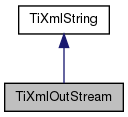
\includegraphics[width=168pt]{class_ti_xml_out_stream__inherit__graph}
\end{center}
\end{figure}


\-Collaboration diagram for \-Ti\-Xml\-Out\-Stream\-:\nopagebreak
\begin{figure}[H]
\begin{center}
\leavevmode
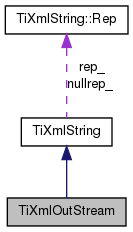
\includegraphics[width=172pt]{class_ti_xml_out_stream__coll__graph}
\end{center}
\end{figure}
\subsection*{\-Public \-Member \-Functions}
\begin{DoxyCompactItemize}
\item 
\hypertarget{class_ti_xml_out_stream_a3640dcb1c0903be3bc6966cdc9a79db6}{\hyperlink{class_ti_xml_out_stream}{\-Ti\-Xml\-Out\-Stream} \& {\bfseries operator$<$$<$} (const \hyperlink{class_ti_xml_string}{\-Ti\-Xml\-String} \&in)}\label{class_ti_xml_out_stream_a3640dcb1c0903be3bc6966cdc9a79db6}

\item 
\hypertarget{class_ti_xml_out_stream_af2117e5a8cbfcb69544804ad2859bfb6}{\hyperlink{class_ti_xml_out_stream}{\-Ti\-Xml\-Out\-Stream} \& {\bfseries operator$<$$<$} (const char $\ast$in)}\label{class_ti_xml_out_stream_af2117e5a8cbfcb69544804ad2859bfb6}

\end{DoxyCompactItemize}


\-The documentation for this class was generated from the following file\-:\begin{DoxyCompactItemize}
\item 
tinyxml/tinystr.\-h\end{DoxyCompactItemize}

\hypertarget{class_ti_xml_parsing_data}{\section{\-Ti\-Xml\-Parsing\-Data \-Class \-Reference}
\label{class_ti_xml_parsing_data}\index{\-Ti\-Xml\-Parsing\-Data@{\-Ti\-Xml\-Parsing\-Data}}
}


\-Collaboration diagram for \-Ti\-Xml\-Parsing\-Data\-:
\nopagebreak
\begin{figure}[H]
\begin{center}
\leavevmode
\includegraphics[width=176pt]{class_ti_xml_parsing_data__coll__graph}
\end{center}
\end{figure}
\subsection*{\-Public \-Member \-Functions}
\begin{DoxyCompactItemize}
\item 
\hypertarget{class_ti_xml_parsing_data_a65cee8ab77a36c605db08c84b4c30a7d}{void {\bfseries \-Stamp} (const char $\ast$now, \-Ti\-Xml\-Encoding encoding)}\label{class_ti_xml_parsing_data_a65cee8ab77a36c605db08c84b4c30a7d}

\item 
\hypertarget{class_ti_xml_parsing_data_a9e63d965fdb53ff4ac711e105269e918}{const \hyperlink{struct_ti_xml_cursor}{\-Ti\-Xml\-Cursor} \& {\bfseries \-Cursor} () const }\label{class_ti_xml_parsing_data_a9e63d965fdb53ff4ac711e105269e918}

\end{DoxyCompactItemize}
\subsection*{\-Private \-Member \-Functions}
\begin{DoxyCompactItemize}
\item 
\hypertarget{class_ti_xml_parsing_data_aa5beaf71579a91d6942277f417899ab9}{{\bfseries \-Ti\-Xml\-Parsing\-Data} (const char $\ast$start, int \-\_\-tabsize, int row, int col)}\label{class_ti_xml_parsing_data_aa5beaf71579a91d6942277f417899ab9}

\end{DoxyCompactItemize}
\subsection*{\-Private \-Attributes}
\begin{DoxyCompactItemize}
\item 
\hypertarget{class_ti_xml_parsing_data_abee4c6c657f595182a4f8beda4fa1c7d}{\hyperlink{struct_ti_xml_cursor}{\-Ti\-Xml\-Cursor} {\bfseries cursor}}\label{class_ti_xml_parsing_data_abee4c6c657f595182a4f8beda4fa1c7d}

\item 
\hypertarget{class_ti_xml_parsing_data_a0e3c2ea5a8b738d733735ca0318fe4ff}{const char $\ast$ {\bfseries stamp}}\label{class_ti_xml_parsing_data_a0e3c2ea5a8b738d733735ca0318fe4ff}

\item 
\hypertarget{class_ti_xml_parsing_data_ab9d6aea2833e38aaef440e49c22a05ca}{int {\bfseries tabsize}}\label{class_ti_xml_parsing_data_ab9d6aea2833e38aaef440e49c22a05ca}

\end{DoxyCompactItemize}
\subsection*{\-Friends}
\begin{DoxyCompactItemize}
\item 
\hypertarget{class_ti_xml_parsing_data_a173617f6dfe902cf484ce5552b950475}{class {\bfseries \-Ti\-Xml\-Document}}\label{class_ti_xml_parsing_data_a173617f6dfe902cf484ce5552b950475}

\end{DoxyCompactItemize}


\-The documentation for this class was generated from the following file\-:\begin{DoxyCompactItemize}
\item 
tinyxml/tinyxmlparser.\-cpp\end{DoxyCompactItemize}

\hypertarget{class_ti_xml_printer}{\section{\-Ti\-Xml\-Printer \-Class \-Reference}
\label{class_ti_xml_printer}\index{\-Ti\-Xml\-Printer@{\-Ti\-Xml\-Printer}}
}


{\ttfamily \#include $<$tinyxml.\-h$>$}



\-Inheritance diagram for \-Ti\-Xml\-Printer\-:\nopagebreak
\begin{figure}[H]
\begin{center}
\leavevmode
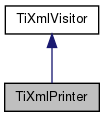
\includegraphics[width=150pt]{class_ti_xml_printer__inherit__graph}
\end{center}
\end{figure}


\-Collaboration diagram for \-Ti\-Xml\-Printer\-:\nopagebreak
\begin{figure}[H]
\begin{center}
\leavevmode
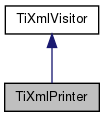
\includegraphics[width=150pt]{class_ti_xml_printer__coll__graph}
\end{center}
\end{figure}
\subsection*{\-Public \-Member \-Functions}
\begin{DoxyCompactItemize}
\item 
\hypertarget{class_ti_xml_printer_a2ec73087db26ff4d2c4316c56f861db7}{virtual bool \hyperlink{class_ti_xml_printer_a2ec73087db26ff4d2c4316c56f861db7}{\-Visit\-Enter} (const \hyperlink{class_ti_xml_document}{\-Ti\-Xml\-Document} \&doc)}\label{class_ti_xml_printer_a2ec73087db26ff4d2c4316c56f861db7}

\begin{DoxyCompactList}\small\item\em \-Visit a document. \end{DoxyCompactList}\item 
\hypertarget{class_ti_xml_printer_a0a636046fa589b6d7f3e5bd025b3f33e}{virtual bool \hyperlink{class_ti_xml_printer_a0a636046fa589b6d7f3e5bd025b3f33e}{\-Visit\-Exit} (const \hyperlink{class_ti_xml_document}{\-Ti\-Xml\-Document} \&doc)}\label{class_ti_xml_printer_a0a636046fa589b6d7f3e5bd025b3f33e}

\begin{DoxyCompactList}\small\item\em \-Visit a document. \end{DoxyCompactList}\item 
\hypertarget{class_ti_xml_printer_a6dccaf5ee4979f13877690afe28721e8}{virtual bool \hyperlink{class_ti_xml_printer_a6dccaf5ee4979f13877690afe28721e8}{\-Visit\-Enter} (const \hyperlink{class_ti_xml_element}{\-Ti\-Xml\-Element} \&element, const \hyperlink{class_ti_xml_attribute}{\-Ti\-Xml\-Attribute} $\ast$first\-Attribute)}\label{class_ti_xml_printer_a6dccaf5ee4979f13877690afe28721e8}

\begin{DoxyCompactList}\small\item\em \-Visit an element. \end{DoxyCompactList}\item 
\hypertarget{class_ti_xml_printer_ae6a1df8271df4bf62d7873c38e34aa69}{virtual bool \hyperlink{class_ti_xml_printer_ae6a1df8271df4bf62d7873c38e34aa69}{\-Visit\-Exit} (const \hyperlink{class_ti_xml_element}{\-Ti\-Xml\-Element} \&element)}\label{class_ti_xml_printer_ae6a1df8271df4bf62d7873c38e34aa69}

\begin{DoxyCompactList}\small\item\em \-Visit an element. \end{DoxyCompactList}\item 
\hypertarget{class_ti_xml_printer_adaf7eec4dc43ad071ff52b60361574f5}{virtual bool \hyperlink{class_ti_xml_printer_adaf7eec4dc43ad071ff52b60361574f5}{\-Visit} (const \hyperlink{class_ti_xml_declaration}{\-Ti\-Xml\-Declaration} \&declaration)}\label{class_ti_xml_printer_adaf7eec4dc43ad071ff52b60361574f5}

\begin{DoxyCompactList}\small\item\em \-Visit a declaration. \end{DoxyCompactList}\item 
\hypertarget{class_ti_xml_printer_a0857c5d32c59b9a257f9a49cb9411df5}{virtual bool \hyperlink{class_ti_xml_printer_a0857c5d32c59b9a257f9a49cb9411df5}{\-Visit} (const \hyperlink{class_ti_xml_text}{\-Ti\-Xml\-Text} \&text)}\label{class_ti_xml_printer_a0857c5d32c59b9a257f9a49cb9411df5}

\begin{DoxyCompactList}\small\item\em \-Visit a text node. \end{DoxyCompactList}\item 
\hypertarget{class_ti_xml_printer_a9870423f5603630e6142f6bdb66dfb57}{virtual bool \hyperlink{class_ti_xml_printer_a9870423f5603630e6142f6bdb66dfb57}{\-Visit} (const \hyperlink{class_ti_xml_comment}{\-Ti\-Xml\-Comment} \&comment)}\label{class_ti_xml_printer_a9870423f5603630e6142f6bdb66dfb57}

\begin{DoxyCompactList}\small\item\em \-Visit a comment node. \end{DoxyCompactList}\item 
\hypertarget{class_ti_xml_printer_a08591a15c9a07afa83c24e08b03d6358}{virtual bool \hyperlink{class_ti_xml_printer_a08591a15c9a07afa83c24e08b03d6358}{\-Visit} (const \hyperlink{class_ti_xml_unknown}{\-Ti\-Xml\-Unknown} \&unknown)}\label{class_ti_xml_printer_a08591a15c9a07afa83c24e08b03d6358}

\begin{DoxyCompactList}\small\item\em \-Visit an unknown node. \end{DoxyCompactList}\item 
void \hyperlink{class_ti_xml_printer_a213377a4070c7e625bae59716b089e5e}{\-Set\-Indent} (const char $\ast$\-\_\-indent)
\item 
\hypertarget{class_ti_xml_printer_abb33ec7d4bad6aaeb57f4304394b133d}{const char $\ast$ \hyperlink{class_ti_xml_printer_abb33ec7d4bad6aaeb57f4304394b133d}{\-Indent} ()}\label{class_ti_xml_printer_abb33ec7d4bad6aaeb57f4304394b133d}

\begin{DoxyCompactList}\small\item\em \-Query the indention string. \end{DoxyCompactList}\item 
void \hyperlink{class_ti_xml_printer_a4be1e37e69e3858c59635aa947174fe6}{\-Set\-Line\-Break} (const char $\ast$\-\_\-line\-Break)
\item 
\hypertarget{class_ti_xml_printer_a11f1b4804a460b175ec244eb5724d96d}{const char $\ast$ \hyperlink{class_ti_xml_printer_a11f1b4804a460b175ec244eb5724d96d}{\-Line\-Break} ()}\label{class_ti_xml_printer_a11f1b4804a460b175ec244eb5724d96d}

\begin{DoxyCompactList}\small\item\em \-Query the current line breaking string. \end{DoxyCompactList}\item 
void \hyperlink{class_ti_xml_printer_ab23a90629e374cb1cadca090468bbd19}{\-Set\-Stream\-Printing} ()
\item 
\hypertarget{class_ti_xml_printer_a859eede9597d3e0355b77757be48735e}{const char $\ast$ \hyperlink{class_ti_xml_printer_a859eede9597d3e0355b77757be48735e}{\-C\-Str} ()}\label{class_ti_xml_printer_a859eede9597d3e0355b77757be48735e}

\begin{DoxyCompactList}\small\item\em \-Return the result. \end{DoxyCompactList}\item 
\hypertarget{class_ti_xml_printer_ad01375ae9199bd2f48252eaddce3039d}{size\-\_\-t \hyperlink{class_ti_xml_printer_ad01375ae9199bd2f48252eaddce3039d}{\-Size} ()}\label{class_ti_xml_printer_ad01375ae9199bd2f48252eaddce3039d}

\begin{DoxyCompactList}\small\item\em \-Return the length of the result string. \end{DoxyCompactList}\end{DoxyCompactItemize}
\subsection*{\-Private \-Member \-Functions}
\begin{DoxyCompactItemize}
\item 
\hypertarget{class_ti_xml_printer_a348ad6527b1d43ddeb51454cddeb6a1d}{void {\bfseries \-Do\-Indent} ()}\label{class_ti_xml_printer_a348ad6527b1d43ddeb51454cddeb6a1d}

\item 
\hypertarget{class_ti_xml_printer_a252a0e13e06def9a06b2eb30a04677a0}{void {\bfseries \-Do\-Line\-Break} ()}\label{class_ti_xml_printer_a252a0e13e06def9a06b2eb30a04677a0}

\end{DoxyCompactItemize}
\subsection*{\-Private \-Attributes}
\begin{DoxyCompactItemize}
\item 
\hypertarget{class_ti_xml_printer_a7e11330449daea912320c22f84387df7}{int {\bfseries depth}}\label{class_ti_xml_printer_a7e11330449daea912320c22f84387df7}

\item 
\hypertarget{class_ti_xml_printer_a2dceede5ae9bb8948f1ecaabb24ab2fb}{bool {\bfseries simple\-Text\-Print}}\label{class_ti_xml_printer_a2dceede5ae9bb8948f1ecaabb24ab2fb}

\item 
\hypertarget{class_ti_xml_printer_ae6cc56c79e52ef352ecc612809fdbedf}{\-T\-I\-X\-M\-L\-\_\-\-S\-T\-R\-I\-N\-G {\bfseries buffer}}\label{class_ti_xml_printer_ae6cc56c79e52ef352ecc612809fdbedf}

\item 
\hypertarget{class_ti_xml_printer_a672fda389bb3f5a2ae8ead867f9a2536}{\-T\-I\-X\-M\-L\-\_\-\-S\-T\-R\-I\-N\-G {\bfseries indent}}\label{class_ti_xml_printer_a672fda389bb3f5a2ae8ead867f9a2536}

\item 
\hypertarget{class_ti_xml_printer_a25e8120bcfda10cc06a11b2dedcef7fe}{\-T\-I\-X\-M\-L\-\_\-\-S\-T\-R\-I\-N\-G {\bfseries line\-Break}}\label{class_ti_xml_printer_a25e8120bcfda10cc06a11b2dedcef7fe}

\end{DoxyCompactItemize}


\subsection{\-Detailed \-Description}
\-Print to memory functionality. \-The \hyperlink{class_ti_xml_printer}{\-Ti\-Xml\-Printer} is useful when you need to\-:


\begin{DoxyEnumerate}
\item \-Print to memory (especially in non-\/\-S\-T\-L mode)
\item \-Control formatting (line endings, etc.)
\end{DoxyEnumerate}

\-When constructed, the \hyperlink{class_ti_xml_printer}{\-Ti\-Xml\-Printer} is in its default \char`\"{}pretty printing\char`\"{} mode. \-Before calling \-Accept() you can call methods to control the printing of the \-X\-M\-L document. \-After \hyperlink{class_ti_xml_node_acc0f88b7462c6cb73809d410a4f5bb86}{\-Ti\-Xml\-Node\-::\-Accept()} is called, the printed document can be accessed via the \hyperlink{class_ti_xml_printer_a859eede9597d3e0355b77757be48735e}{\-C\-Str()}, \-Str(), and \hyperlink{class_ti_xml_printer_ad01375ae9199bd2f48252eaddce3039d}{\-Size()} methods.

\hyperlink{class_ti_xml_printer}{\-Ti\-Xml\-Printer} uses the \-Visitor \-A\-P\-I. \begin{DoxyVerb}
	TiXmlPrinter printer;
	printer.SetIndent( "\t" );

	doc.Accept( &printer );
	fprintf( stdout, "%s", printer.CStr() );
	\end{DoxyVerb}
 

\subsection{\-Member \-Function \-Documentation}
\hypertarget{class_ti_xml_printer_a213377a4070c7e625bae59716b089e5e}{\index{\-Ti\-Xml\-Printer@{\-Ti\-Xml\-Printer}!\-Set\-Indent@{\-Set\-Indent}}
\index{\-Set\-Indent@{\-Set\-Indent}!TiXmlPrinter@{\-Ti\-Xml\-Printer}}
\subsubsection[{\-Set\-Indent}]{\setlength{\rightskip}{0pt plus 5cm}void {\bf \-Ti\-Xml\-Printer\-::\-Set\-Indent} (
\begin{DoxyParamCaption}
\item[{const char $\ast$}]{\-\_\-indent}
\end{DoxyParamCaption}
)\hspace{0.3cm}{\ttfamily  \mbox{[}inline\mbox{]}}}}\label{class_ti_xml_printer_a213377a4070c7e625bae59716b089e5e}
\-Set the indent characters for printing. \-By default 4 spaces but tab () is also useful, or null/empty string for no indentation. \hypertarget{class_ti_xml_printer_a4be1e37e69e3858c59635aa947174fe6}{\index{\-Ti\-Xml\-Printer@{\-Ti\-Xml\-Printer}!\-Set\-Line\-Break@{\-Set\-Line\-Break}}
\index{\-Set\-Line\-Break@{\-Set\-Line\-Break}!TiXmlPrinter@{\-Ti\-Xml\-Printer}}
\subsubsection[{\-Set\-Line\-Break}]{\setlength{\rightskip}{0pt plus 5cm}void {\bf \-Ti\-Xml\-Printer\-::\-Set\-Line\-Break} (
\begin{DoxyParamCaption}
\item[{const char $\ast$}]{\-\_\-line\-Break}
\end{DoxyParamCaption}
)\hspace{0.3cm}{\ttfamily  \mbox{[}inline\mbox{]}}}}\label{class_ti_xml_printer_a4be1e37e69e3858c59635aa947174fe6}
\-Set the line breaking string. \-By default set to newline (\par
). \-Some operating systems prefer other characters, or can be set to the null/empty string for no indenation. \hypertarget{class_ti_xml_printer_ab23a90629e374cb1cadca090468bbd19}{\index{\-Ti\-Xml\-Printer@{\-Ti\-Xml\-Printer}!\-Set\-Stream\-Printing@{\-Set\-Stream\-Printing}}
\index{\-Set\-Stream\-Printing@{\-Set\-Stream\-Printing}!TiXmlPrinter@{\-Ti\-Xml\-Printer}}
\subsubsection[{\-Set\-Stream\-Printing}]{\setlength{\rightskip}{0pt plus 5cm}void {\bf \-Ti\-Xml\-Printer\-::\-Set\-Stream\-Printing} (
\begin{DoxyParamCaption}
{}
\end{DoxyParamCaption}
)\hspace{0.3cm}{\ttfamily  \mbox{[}inline\mbox{]}}}}\label{class_ti_xml_printer_ab23a90629e374cb1cadca090468bbd19}
\-Switch over to \char`\"{}stream printing\char`\"{} which is the most dense formatting without linebreaks. \-Common when the \-X\-M\-L is needed for network transmission. 

\-The documentation for this class was generated from the following files\-:\begin{DoxyCompactItemize}
\item 
tinyxml/tinyxml.\-h\item 
tinyxml/tinyxml.\-cpp\end{DoxyCompactItemize}

\hypertarget{class_ti_xml_string}{\section{\-Ti\-Xml\-String \-Class \-Reference}
\label{class_ti_xml_string}\index{\-Ti\-Xml\-String@{\-Ti\-Xml\-String}}
}


\-Inheritance diagram for \-Ti\-Xml\-String\-:\nopagebreak
\begin{figure}[H]
\begin{center}
\leavevmode
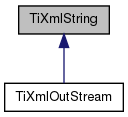
\includegraphics[width=168pt]{class_ti_xml_string__inherit__graph}
\end{center}
\end{figure}


\-Collaboration diagram for \-Ti\-Xml\-String\-:\nopagebreak
\begin{figure}[H]
\begin{center}
\leavevmode
\includegraphics[width=172pt]{class_ti_xml_string__coll__graph}
\end{center}
\end{figure}
\subsection*{\-Classes}
\begin{DoxyCompactItemize}
\item 
struct \hyperlink{struct_ti_xml_string_1_1_rep}{\-Rep}
\end{DoxyCompactItemize}
\subsection*{\-Public \-Types}
\begin{DoxyCompactItemize}
\item 
\hypertarget{class_ti_xml_string_abeb2c1893a04c17904f7c06546d0b971}{typedef size\-\_\-t {\bfseries size\-\_\-type}}\label{class_ti_xml_string_abeb2c1893a04c17904f7c06546d0b971}

\end{DoxyCompactItemize}
\subsection*{\-Public \-Member \-Functions}
\begin{DoxyCompactItemize}
\item 
\hypertarget{class_ti_xml_string_ac80fe17693a438c9ab2591664743fcb6}{{\bfseries \-Ti\-Xml\-String} (const \hyperlink{class_ti_xml_string}{\-Ti\-Xml\-String} \&copy)}\label{class_ti_xml_string_ac80fe17693a438c9ab2591664743fcb6}

\item 
\hypertarget{class_ti_xml_string_aa3b32bd2891a757c9f36c21db44c81d2}{\-T\-I\-X\-M\-L\-\_\-\-E\-X\-P\-L\-I\-C\-I\-T {\bfseries \-Ti\-Xml\-String} (const char $\ast$copy)}\label{class_ti_xml_string_aa3b32bd2891a757c9f36c21db44c81d2}

\item 
\hypertarget{class_ti_xml_string_a4b17ea5c5db986f14827223dfa8f1547}{\-T\-I\-X\-M\-L\-\_\-\-E\-X\-P\-L\-I\-C\-I\-T {\bfseries \-Ti\-Xml\-String} (const char $\ast$str, size\-\_\-type len)}\label{class_ti_xml_string_a4b17ea5c5db986f14827223dfa8f1547}

\item 
\hypertarget{class_ti_xml_string_ae0bc6147afc0ec2aa0da3a3c0a8fcfb0}{\hyperlink{class_ti_xml_string}{\-Ti\-Xml\-String} \& {\bfseries operator=} (const char $\ast$copy)}\label{class_ti_xml_string_ae0bc6147afc0ec2aa0da3a3c0a8fcfb0}

\item 
\hypertarget{class_ti_xml_string_ab1f1f5d3eceaa0f22d0a7e6055ea81b0}{\hyperlink{class_ti_xml_string}{\-Ti\-Xml\-String} \& {\bfseries operator=} (const \hyperlink{class_ti_xml_string}{\-Ti\-Xml\-String} \&copy)}\label{class_ti_xml_string_ab1f1f5d3eceaa0f22d0a7e6055ea81b0}

\item 
\hypertarget{class_ti_xml_string_ab56336ac2aa2a08d24a71eb9a2b502a5}{\hyperlink{class_ti_xml_string}{\-Ti\-Xml\-String} \& {\bfseries operator+=} (const char $\ast$suffix)}\label{class_ti_xml_string_ab56336ac2aa2a08d24a71eb9a2b502a5}

\item 
\hypertarget{class_ti_xml_string_a6aa09d5240470b76d54ec709e04f8c13}{\hyperlink{class_ti_xml_string}{\-Ti\-Xml\-String} \& {\bfseries operator+=} (char single)}\label{class_ti_xml_string_a6aa09d5240470b76d54ec709e04f8c13}

\item 
\hypertarget{class_ti_xml_string_afdcae5ea2b4d9e194dc21226b817f417}{\hyperlink{class_ti_xml_string}{\-Ti\-Xml\-String} \& {\bfseries operator+=} (const \hyperlink{class_ti_xml_string}{\-Ti\-Xml\-String} \&suffix)}\label{class_ti_xml_string_afdcae5ea2b4d9e194dc21226b817f417}

\item 
\hypertarget{class_ti_xml_string_a5581ca641d915551d3cda90f8e7bf49b}{const char $\ast$ {\bfseries c\-\_\-str} () const }\label{class_ti_xml_string_a5581ca641d915551d3cda90f8e7bf49b}

\item 
\hypertarget{class_ti_xml_string_a00abc60f135c7ca1951c7334cc2c7993}{const char $\ast$ {\bfseries data} () const }\label{class_ti_xml_string_a00abc60f135c7ca1951c7334cc2c7993}

\item 
\hypertarget{class_ti_xml_string_a3202f27d139a3fac79205f1f3c707727}{size\-\_\-type {\bfseries length} () const }\label{class_ti_xml_string_a3202f27d139a3fac79205f1f3c707727}

\item 
\hypertarget{class_ti_xml_string_a96103e5c0f67e987fa48527e1f47a1f6}{size\-\_\-type {\bfseries size} () const }\label{class_ti_xml_string_a96103e5c0f67e987fa48527e1f47a1f6}

\item 
\hypertarget{class_ti_xml_string_a9a61e1d11cdb71bea4a4ed79caa793f4}{bool {\bfseries empty} () const }\label{class_ti_xml_string_a9a61e1d11cdb71bea4a4ed79caa793f4}

\item 
\hypertarget{class_ti_xml_string_a76e4d6aba7845f4cf9c02332a5fbf916}{size\-\_\-type {\bfseries capacity} () const }\label{class_ti_xml_string_a76e4d6aba7845f4cf9c02332a5fbf916}

\item 
\hypertarget{class_ti_xml_string_a6763093267bbdecbf03f8840bc349877}{const char \& {\bfseries at} (size\-\_\-type index) const }\label{class_ti_xml_string_a6763093267bbdecbf03f8840bc349877}

\item 
\hypertarget{class_ti_xml_string_ae8cdc1d46c538536b786f7ae03c0c1d9}{char \& {\bfseries operator\mbox{[}$\,$\mbox{]}} (size\-\_\-type index) const }\label{class_ti_xml_string_ae8cdc1d46c538536b786f7ae03c0c1d9}

\item 
\hypertarget{class_ti_xml_string_a5c2b368b5eafe075fd9565cbcbd4c2f9}{size\-\_\-type {\bfseries find} (char lookup) const }\label{class_ti_xml_string_a5c2b368b5eafe075fd9565cbcbd4c2f9}

\item 
\hypertarget{class_ti_xml_string_a5f2a6fd565751410b392f249a9786db4}{size\-\_\-type {\bfseries find} (char tofind, size\-\_\-type offset) const }\label{class_ti_xml_string_a5f2a6fd565751410b392f249a9786db4}

\item 
\hypertarget{class_ti_xml_string_ab20e06e4c666abf3bdbfb3a1191d4888}{void {\bfseries clear} ()}\label{class_ti_xml_string_ab20e06e4c666abf3bdbfb3a1191d4888}

\item 
\hypertarget{class_ti_xml_string_a88ecf9f0f00cb5c67b6b637958d7049c}{void {\bfseries reserve} (size\-\_\-type cap)}\label{class_ti_xml_string_a88ecf9f0f00cb5c67b6b637958d7049c}

\item 
\hypertarget{class_ti_xml_string_ac72f3d9149b7812c1e6c59402014d0d5}{\hyperlink{class_ti_xml_string}{\-Ti\-Xml\-String} \& {\bfseries assign} (const char $\ast$str, size\-\_\-type len)}\label{class_ti_xml_string_ac72f3d9149b7812c1e6c59402014d0d5}

\item 
\hypertarget{class_ti_xml_string_ad44b21700d2ec24a511367b222b643fb}{\hyperlink{class_ti_xml_string}{\-Ti\-Xml\-String} \& {\bfseries append} (const char $\ast$str, size\-\_\-type len)}\label{class_ti_xml_string_ad44b21700d2ec24a511367b222b643fb}

\item 
\hypertarget{class_ti_xml_string_aa392cbc180752a79f007f4f9280c7762}{void {\bfseries swap} (\hyperlink{class_ti_xml_string}{\-Ti\-Xml\-String} \&other)}\label{class_ti_xml_string_aa392cbc180752a79f007f4f9280c7762}

\end{DoxyCompactItemize}
\subsection*{\-Static \-Public \-Attributes}
\begin{DoxyCompactItemize}
\item 
\hypertarget{class_ti_xml_string_a8f4422d227088dc7bec96f479b275d0a}{static const size\-\_\-type {\bfseries npos} = static\-\_\-cast$<$ \-Ti\-Xml\-String\-::size\-\_\-type $>$(-\/1)}\label{class_ti_xml_string_a8f4422d227088dc7bec96f479b275d0a}

\end{DoxyCompactItemize}
\subsection*{\-Private \-Member \-Functions}
\begin{DoxyCompactItemize}
\item 
\hypertarget{class_ti_xml_string_a694eacb51c43d8eba8aa7d4552b598ff}{void {\bfseries init} (size\-\_\-type sz)}\label{class_ti_xml_string_a694eacb51c43d8eba8aa7d4552b598ff}

\item 
\hypertarget{class_ti_xml_string_a5d70615367bf2920c25feddf6ac4ad30}{void {\bfseries set\-\_\-size} (size\-\_\-type sz)}\label{class_ti_xml_string_a5d70615367bf2920c25feddf6ac4ad30}

\item 
\hypertarget{class_ti_xml_string_a36417caceebe25352f53a87e8cd966b4}{char $\ast$ {\bfseries start} () const }\label{class_ti_xml_string_a36417caceebe25352f53a87e8cd966b4}

\item 
\hypertarget{class_ti_xml_string_a58faf1c6b9828c8d5d5092bebf146167}{char $\ast$ {\bfseries finish} () const }\label{class_ti_xml_string_a58faf1c6b9828c8d5d5092bebf146167}

\item 
\hypertarget{class_ti_xml_string_ae11cd23e090fd2e7bb62eda05b45a2d6}{void {\bfseries init} (size\-\_\-type sz, size\-\_\-type cap)}\label{class_ti_xml_string_ae11cd23e090fd2e7bb62eda05b45a2d6}

\item 
\hypertarget{class_ti_xml_string_aa6008ae51286a342cd366fbf1e3eeafc}{void {\bfseries quit} ()}\label{class_ti_xml_string_aa6008ae51286a342cd366fbf1e3eeafc}

\end{DoxyCompactItemize}
\subsection*{\-Private \-Attributes}
\begin{DoxyCompactItemize}
\item 
\hypertarget{class_ti_xml_string_ac7be48f31ca451bcb16de428b5c40e0c}{\hyperlink{struct_ti_xml_string_1_1_rep}{\-Rep} $\ast$ {\bfseries rep\-\_\-}}\label{class_ti_xml_string_ac7be48f31ca451bcb16de428b5c40e0c}

\end{DoxyCompactItemize}
\subsection*{\-Static \-Private \-Attributes}
\begin{DoxyCompactItemize}
\item 
\hypertarget{class_ti_xml_string_ae1f9e0de28328eed27d5623ff67a3191}{static \hyperlink{struct_ti_xml_string_1_1_rep}{\-Rep} {\bfseries nullrep\-\_\-} = \{ 0, 0, \{ '$\backslash$0' \} \}}\label{class_ti_xml_string_ae1f9e0de28328eed27d5623ff67a3191}

\end{DoxyCompactItemize}


\-The documentation for this class was generated from the following files\-:\begin{DoxyCompactItemize}
\item 
tinyxml/tinystr.\-h\item 
tinyxml/tinystr.\-cpp\end{DoxyCompactItemize}

\hypertarget{class_ti_xml_text}{\section{\-Ti\-Xml\-Text \-Class \-Reference}
\label{class_ti_xml_text}\index{\-Ti\-Xml\-Text@{\-Ti\-Xml\-Text}}
}


{\ttfamily \#include $<$tinyxml.\-h$>$}



\-Inheritance diagram for \-Ti\-Xml\-Text\-:
\nopagebreak
\begin{figure}[H]
\begin{center}
\leavevmode
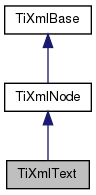
\includegraphics[width=144pt]{class_ti_xml_text__inherit__graph}
\end{center}
\end{figure}


\-Collaboration diagram for \-Ti\-Xml\-Text\-:
\nopagebreak
\begin{figure}[H]
\begin{center}
\leavevmode
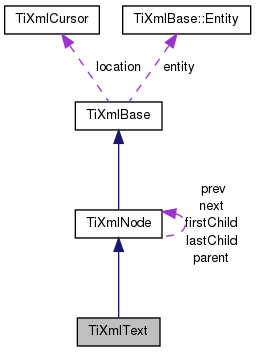
\includegraphics[width=205pt]{class_ti_xml_text__coll__graph}
\end{center}
\end{figure}
\subsection*{\-Public \-Member \-Functions}
\begin{DoxyCompactItemize}
\item 
\hyperlink{class_ti_xml_text_af659e77c6b87d684827f35a8f4895960}{\-Ti\-Xml\-Text} (const char $\ast$init\-Value)
\item 
\hypertarget{class_ti_xml_text_a8d2cc1b4af2208cbb0171cf20f6815d1}{{\bfseries \-Ti\-Xml\-Text} (const \hyperlink{class_ti_xml_text}{\-Ti\-Xml\-Text} \&copy)}\label{class_ti_xml_text_a8d2cc1b4af2208cbb0171cf20f6815d1}

\item 
\hypertarget{class_ti_xml_text_aed5b13f9c1b804c616fd533882c29f57}{\hyperlink{class_ti_xml_text}{\-Ti\-Xml\-Text} \& {\bfseries operator=} (const \hyperlink{class_ti_xml_text}{\-Ti\-Xml\-Text} \&base)}\label{class_ti_xml_text_aed5b13f9c1b804c616fd533882c29f57}

\item 
virtual void \hyperlink{class_ti_xml_text_ae74d56c5b3ddec6cc3103dd51821af92}{\-Print} (\-F\-I\-L\-E $\ast$cfile, int depth) const 
\item 
\hypertarget{class_ti_xml_text_ad1a6a6b83fa2271022dd97c072a2b586}{bool \hyperlink{class_ti_xml_text_ad1a6a6b83fa2271022dd97c072a2b586}{\-C\-D\-A\-T\-A} () const }\label{class_ti_xml_text_ad1a6a6b83fa2271022dd97c072a2b586}

\begin{DoxyCompactList}\small\item\em \-Queries whether this represents text using a \-C\-D\-A\-T\-A section. \end{DoxyCompactList}\item 
\hypertarget{class_ti_xml_text_acb17ff7c5d09b2c839393445a3de5ea9}{void \hyperlink{class_ti_xml_text_acb17ff7c5d09b2c839393445a3de5ea9}{\-Set\-C\-D\-A\-T\-A} (bool \-\_\-cdata)}\label{class_ti_xml_text_acb17ff7c5d09b2c839393445a3de5ea9}

\begin{DoxyCompactList}\small\item\em \-Turns on or off a \-C\-D\-A\-T\-A representation of text. \end{DoxyCompactList}\item 
\hypertarget{class_ti_xml_text_a8d2dcfa41fc73d3e62dacc2fcf633819}{virtual const char $\ast$ {\bfseries \-Parse} (const char $\ast$p, \hyperlink{class_ti_xml_parsing_data}{\-Ti\-Xml\-Parsing\-Data} $\ast$data, \-Ti\-Xml\-Encoding encoding)}\label{class_ti_xml_text_a8d2dcfa41fc73d3e62dacc2fcf633819}

\item 
\hypertarget{class_ti_xml_text_a895bf34ffad17f7439ab2a52b9651648}{virtual const \hyperlink{class_ti_xml_text}{\-Ti\-Xml\-Text} $\ast$ \hyperlink{class_ti_xml_text_a895bf34ffad17f7439ab2a52b9651648}{\-To\-Text} () const }\label{class_ti_xml_text_a895bf34ffad17f7439ab2a52b9651648}

\begin{DoxyCompactList}\small\item\em \-Cast to a more defined type. \-Will return null not of the requested type. \end{DoxyCompactList}\item 
\hypertarget{class_ti_xml_text_ae7c3a8fd3e4dbf6c0c4363a943d72f5b}{virtual \hyperlink{class_ti_xml_text}{\-Ti\-Xml\-Text} $\ast$ \hyperlink{class_ti_xml_text_ae7c3a8fd3e4dbf6c0c4363a943d72f5b}{\-To\-Text} ()}\label{class_ti_xml_text_ae7c3a8fd3e4dbf6c0c4363a943d72f5b}

\begin{DoxyCompactList}\small\item\em \-Cast to a more defined type. \-Will return null not of the requested type. \end{DoxyCompactList}\item 
virtual bool \hyperlink{class_ti_xml_text_a43b9954ebf679557fac1a4453f337b7c}{\-Accept} (\hyperlink{class_ti_xml_visitor}{\-Ti\-Xml\-Visitor} $\ast$content) const 
\end{DoxyCompactItemize}
\subsection*{\-Protected \-Member \-Functions}
\begin{DoxyCompactItemize}
\item 
\hypertarget{class_ti_xml_text_adde1869dfb029be50713fbfd8ce4d21f}{virtual \hyperlink{class_ti_xml_node}{\-Ti\-Xml\-Node} $\ast$ \hyperlink{class_ti_xml_text_adde1869dfb029be50713fbfd8ce4d21f}{\-Clone} () const }\label{class_ti_xml_text_adde1869dfb029be50713fbfd8ce4d21f}

\begin{DoxyCompactList}\small\item\em \mbox{[}internal use\mbox{]} \-Creates a new \-Element and returns it. \end{DoxyCompactList}\item 
\hypertarget{class_ti_xml_text_adcec7d9b6fccfc5777452bb97e6031c1}{void {\bfseries \-Copy\-To} (\hyperlink{class_ti_xml_text}{\-Ti\-Xml\-Text} $\ast$target) const }\label{class_ti_xml_text_adcec7d9b6fccfc5777452bb97e6031c1}

\item 
\hypertarget{class_ti_xml_text_a1c120428e3b3cf24d79706e6d2b65aa6}{bool {\bfseries \-Blank} () const }\label{class_ti_xml_text_a1c120428e3b3cf24d79706e6d2b65aa6}

\end{DoxyCompactItemize}
\subsection*{\-Friends}
\begin{DoxyCompactItemize}
\item 
\hypertarget{class_ti_xml_text_ab6592e32cb9132be517cc12a70564c4b}{class {\bfseries \-Ti\-Xml\-Element}}\label{class_ti_xml_text_ab6592e32cb9132be517cc12a70564c4b}

\end{DoxyCompactItemize}


\subsection{\-Detailed \-Description}
\-X\-M\-L text. \-A text node can have 2 ways to output the next. \char`\"{}normal\char`\"{} output and \-C\-D\-A\-T\-A. \-It will default to the mode it was parsed from the \-X\-M\-L file and you generally want to leave it alone, but you can change the output mode with \hyperlink{class_ti_xml_text_acb17ff7c5d09b2c839393445a3de5ea9}{\-Set\-C\-D\-A\-T\-A()} and query it with \hyperlink{class_ti_xml_text_ad1a6a6b83fa2271022dd97c072a2b586}{\-C\-D\-A\-T\-A()}. 

\subsection{\-Constructor \& \-Destructor \-Documentation}
\hypertarget{class_ti_xml_text_af659e77c6b87d684827f35a8f4895960}{\index{\-Ti\-Xml\-Text@{\-Ti\-Xml\-Text}!\-Ti\-Xml\-Text@{\-Ti\-Xml\-Text}}
\index{\-Ti\-Xml\-Text@{\-Ti\-Xml\-Text}!TiXmlText@{\-Ti\-Xml\-Text}}
\subsubsection[{\-Ti\-Xml\-Text}]{\setlength{\rightskip}{0pt plus 5cm}{\bf \-Ti\-Xml\-Text\-::\-Ti\-Xml\-Text} (
\begin{DoxyParamCaption}
\item[{const char $\ast$}]{init\-Value}
\end{DoxyParamCaption}
)\hspace{0.3cm}{\ttfamily  \mbox{[}inline\mbox{]}}}}\label{class_ti_xml_text_af659e77c6b87d684827f35a8f4895960}
\-Constructor for text element. \-By default, it is treated as normal, encoded text. \-If you want it be output as a \-C\-D\-A\-T\-A text element, set the parameter \-\_\-cdata to 'true' 

\subsection{\-Member \-Function \-Documentation}
\hypertarget{class_ti_xml_text_a43b9954ebf679557fac1a4453f337b7c}{\index{\-Ti\-Xml\-Text@{\-Ti\-Xml\-Text}!\-Accept@{\-Accept}}
\index{\-Accept@{\-Accept}!TiXmlText@{\-Ti\-Xml\-Text}}
\subsubsection[{\-Accept}]{\setlength{\rightskip}{0pt plus 5cm}bool {\bf \-Ti\-Xml\-Text\-::\-Accept} (
\begin{DoxyParamCaption}
\item[{{\bf \-Ti\-Xml\-Visitor} $\ast$}]{content}
\end{DoxyParamCaption}
) const\hspace{0.3cm}{\ttfamily  \mbox{[}virtual\mbox{]}}}}\label{class_ti_xml_text_a43b9954ebf679557fac1a4453f337b7c}
\-Walk the \-X\-M\-L tree visiting this node and all of its children. 

\-Implements \hyperlink{class_ti_xml_node_acc0f88b7462c6cb73809d410a4f5bb86}{\-Ti\-Xml\-Node}.

\hypertarget{class_ti_xml_text_ae74d56c5b3ddec6cc3103dd51821af92}{\index{\-Ti\-Xml\-Text@{\-Ti\-Xml\-Text}!\-Print@{\-Print}}
\index{\-Print@{\-Print}!TiXmlText@{\-Ti\-Xml\-Text}}
\subsubsection[{\-Print}]{\setlength{\rightskip}{0pt plus 5cm}void {\bf \-Ti\-Xml\-Text\-::\-Print} (
\begin{DoxyParamCaption}
\item[{\-F\-I\-L\-E $\ast$}]{cfile, }
\item[{int}]{depth}
\end{DoxyParamCaption}
) const\hspace{0.3cm}{\ttfamily  \mbox{[}virtual\mbox{]}}}}\label{class_ti_xml_text_ae74d56c5b3ddec6cc3103dd51821af92}
\-All \-Tiny\-Xml classes can print themselves to a filestream or the string class (\hyperlink{class_ti_xml_string}{\-Ti\-Xml\-String} in non-\/\-S\-T\-L mode, std\-::string in \-S\-T\-L mode.) \-Either or both cfile and str can be null.

\-This is a formatted print, and will insert tabs and newlines.

(\-For an unformatted stream, use the $<$$<$ operator.) 

\-Implements \hyperlink{class_ti_xml_base_a0de56b3f2ef14c65091a3b916437b512}{\-Ti\-Xml\-Base}.



\-The documentation for this class was generated from the following files\-:\begin{DoxyCompactItemize}
\item 
tinyxml/tinyxml.\-h\item 
tinyxml/tinyxml.\-cpp\item 
tinyxml/tinyxmlparser.\-cpp\end{DoxyCompactItemize}

\hypertarget{class_ti_xml_unknown}{\section{\-Ti\-Xml\-Unknown \-Class \-Reference}
\label{class_ti_xml_unknown}\index{\-Ti\-Xml\-Unknown@{\-Ti\-Xml\-Unknown}}
}


{\ttfamily \#include $<$tinyxml.\-h$>$}



\-Inheritance diagram for \-Ti\-Xml\-Unknown\-:
\nopagebreak
\begin{figure}[H]
\begin{center}
\leavevmode
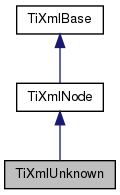
\includegraphics[width=162pt]{class_ti_xml_unknown__inherit__graph}
\end{center}
\end{figure}


\-Collaboration diagram for \-Ti\-Xml\-Unknown\-:
\nopagebreak
\begin{figure}[H]
\begin{center}
\leavevmode
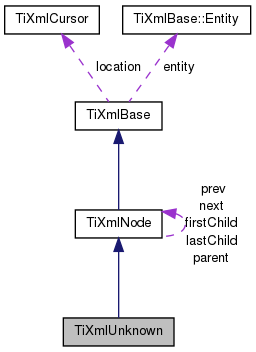
\includegraphics[width=211pt]{class_ti_xml_unknown__coll__graph}
\end{center}
\end{figure}
\subsection*{\-Public \-Member \-Functions}
\begin{DoxyCompactItemize}
\item 
\hypertarget{class_ti_xml_unknown_abe798ff4feea31474850c7f0de6bdf5e}{{\bfseries \-Ti\-Xml\-Unknown} (const \hyperlink{class_ti_xml_unknown}{\-Ti\-Xml\-Unknown} \&copy)}\label{class_ti_xml_unknown_abe798ff4feea31474850c7f0de6bdf5e}

\item 
\hypertarget{class_ti_xml_unknown_a60560b5aacb4bdc8b2b5f02f0a99c5c0}{\hyperlink{class_ti_xml_unknown}{\-Ti\-Xml\-Unknown} \& {\bfseries operator=} (const \hyperlink{class_ti_xml_unknown}{\-Ti\-Xml\-Unknown} \&copy)}\label{class_ti_xml_unknown_a60560b5aacb4bdc8b2b5f02f0a99c5c0}

\item 
\hypertarget{class_ti_xml_unknown_a675c4b2684af35e4c7649b7fd5ae598d}{virtual \hyperlink{class_ti_xml_node}{\-Ti\-Xml\-Node} $\ast$ \hyperlink{class_ti_xml_unknown_a675c4b2684af35e4c7649b7fd5ae598d}{\-Clone} () const }\label{class_ti_xml_unknown_a675c4b2684af35e4c7649b7fd5ae598d}

\begin{DoxyCompactList}\small\item\em \-Creates a copy of this \-Unknown and returns it. \end{DoxyCompactList}\item 
virtual void \hyperlink{class_ti_xml_unknown_a025f19c21ef01ea9be50febb8fe0ba06}{\-Print} (\-F\-I\-L\-E $\ast$cfile, int depth) const 
\item 
\hypertarget{class_ti_xml_unknown_aa51c2694e4177b5f0b5429ee5a81b58d}{virtual const char $\ast$ {\bfseries \-Parse} (const char $\ast$p, \hyperlink{class_ti_xml_parsing_data}{\-Ti\-Xml\-Parsing\-Data} $\ast$data, \-Ti\-Xml\-Encoding encoding)}\label{class_ti_xml_unknown_aa51c2694e4177b5f0b5429ee5a81b58d}

\item 
\hypertarget{class_ti_xml_unknown_ab0313e5fe77987d746ac1a97a254419d}{virtual const \hyperlink{class_ti_xml_unknown}{\-Ti\-Xml\-Unknown} $\ast$ \hyperlink{class_ti_xml_unknown_ab0313e5fe77987d746ac1a97a254419d}{\-To\-Unknown} () const }\label{class_ti_xml_unknown_ab0313e5fe77987d746ac1a97a254419d}

\begin{DoxyCompactList}\small\item\em \-Cast to a more defined type. \-Will return null not of the requested type. \end{DoxyCompactList}\item 
\hypertarget{class_ti_xml_unknown_a67c9fd22940e8c47f706a72cdd2e332c}{virtual \hyperlink{class_ti_xml_unknown}{\-Ti\-Xml\-Unknown} $\ast$ \hyperlink{class_ti_xml_unknown_a67c9fd22940e8c47f706a72cdd2e332c}{\-To\-Unknown} ()}\label{class_ti_xml_unknown_a67c9fd22940e8c47f706a72cdd2e332c}

\begin{DoxyCompactList}\small\item\em \-Cast to a more defined type. \-Will return null not of the requested type. \end{DoxyCompactList}\item 
virtual bool \hyperlink{class_ti_xml_unknown_a4e54d7482e05a837cf83c925cc683380}{\-Accept} (\hyperlink{class_ti_xml_visitor}{\-Ti\-Xml\-Visitor} $\ast$content) const 
\end{DoxyCompactItemize}
\subsection*{\-Protected \-Member \-Functions}
\begin{DoxyCompactItemize}
\item 
\hypertarget{class_ti_xml_unknown_a08ca7b225a2bcb604d3c72e199d33408}{void {\bfseries \-Copy\-To} (\hyperlink{class_ti_xml_unknown}{\-Ti\-Xml\-Unknown} $\ast$target) const }\label{class_ti_xml_unknown_a08ca7b225a2bcb604d3c72e199d33408}

\end{DoxyCompactItemize}


\subsection{\-Detailed \-Description}
\-Any tag that tiny\-Xml doesn't recognize is saved as an unknown. \-It is a tag of text, but should not be modified. \-It will be written back to the \-X\-M\-L, unchanged, when the file is saved.

\-D\-T\-D tags get thrown into \-Ti\-Xml\-Unknowns. 

\subsection{\-Member \-Function \-Documentation}
\hypertarget{class_ti_xml_unknown_a4e54d7482e05a837cf83c925cc683380}{\index{\-Ti\-Xml\-Unknown@{\-Ti\-Xml\-Unknown}!\-Accept@{\-Accept}}
\index{\-Accept@{\-Accept}!TiXmlUnknown@{\-Ti\-Xml\-Unknown}}
\subsubsection[{\-Accept}]{\setlength{\rightskip}{0pt plus 5cm}bool {\bf \-Ti\-Xml\-Unknown\-::\-Accept} (
\begin{DoxyParamCaption}
\item[{{\bf \-Ti\-Xml\-Visitor} $\ast$}]{content}
\end{DoxyParamCaption}
) const\hspace{0.3cm}{\ttfamily  \mbox{[}virtual\mbox{]}}}}\label{class_ti_xml_unknown_a4e54d7482e05a837cf83c925cc683380}
\-Walk the \-X\-M\-L tree visiting this node and all of its children. 

\-Implements \hyperlink{class_ti_xml_node_acc0f88b7462c6cb73809d410a4f5bb86}{\-Ti\-Xml\-Node}.

\hypertarget{class_ti_xml_unknown_a025f19c21ef01ea9be50febb8fe0ba06}{\index{\-Ti\-Xml\-Unknown@{\-Ti\-Xml\-Unknown}!\-Print@{\-Print}}
\index{\-Print@{\-Print}!TiXmlUnknown@{\-Ti\-Xml\-Unknown}}
\subsubsection[{\-Print}]{\setlength{\rightskip}{0pt plus 5cm}void {\bf \-Ti\-Xml\-Unknown\-::\-Print} (
\begin{DoxyParamCaption}
\item[{\-F\-I\-L\-E $\ast$}]{cfile, }
\item[{int}]{depth}
\end{DoxyParamCaption}
) const\hspace{0.3cm}{\ttfamily  \mbox{[}virtual\mbox{]}}}}\label{class_ti_xml_unknown_a025f19c21ef01ea9be50febb8fe0ba06}
\-All \-Tiny\-Xml classes can print themselves to a filestream or the string class (\hyperlink{class_ti_xml_string}{\-Ti\-Xml\-String} in non-\/\-S\-T\-L mode, std\-::string in \-S\-T\-L mode.) \-Either or both cfile and str can be null.

\-This is a formatted print, and will insert tabs and newlines.

(\-For an unformatted stream, use the $<$$<$ operator.) 

\-Implements \hyperlink{class_ti_xml_base_a0de56b3f2ef14c65091a3b916437b512}{\-Ti\-Xml\-Base}.



\-The documentation for this class was generated from the following files\-:\begin{DoxyCompactItemize}
\item 
tinyxml/tinyxml.\-h\item 
tinyxml/tinyxml.\-cpp\item 
tinyxml/tinyxmlparser.\-cpp\end{DoxyCompactItemize}

\hypertarget{class_ti_xml_visitor}{\section{\-Ti\-Xml\-Visitor \-Class \-Reference}
\label{class_ti_xml_visitor}\index{\-Ti\-Xml\-Visitor@{\-Ti\-Xml\-Visitor}}
}


{\ttfamily \#include $<$tinyxml.\-h$>$}



\-Inheritance diagram for \-Ti\-Xml\-Visitor\-:
\nopagebreak
\begin{figure}[H]
\begin{center}
\leavevmode
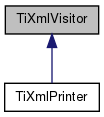
\includegraphics[width=150pt]{class_ti_xml_visitor__inherit__graph}
\end{center}
\end{figure}
\subsection*{\-Public \-Member \-Functions}
\begin{DoxyCompactItemize}
\item 
\hypertarget{class_ti_xml_visitor_a07baecb52dd7d8716ae2a48ad0956ee0}{virtual bool \hyperlink{class_ti_xml_visitor_a07baecb52dd7d8716ae2a48ad0956ee0}{\-Visit\-Enter} (const \hyperlink{class_ti_xml_document}{\-Ti\-Xml\-Document} \&)}\label{class_ti_xml_visitor_a07baecb52dd7d8716ae2a48ad0956ee0}

\begin{DoxyCompactList}\small\item\em \-Visit a document. \end{DoxyCompactList}\item 
\hypertarget{class_ti_xml_visitor_aa0ade4f27087447e93974e975c3246ad}{virtual bool \hyperlink{class_ti_xml_visitor_aa0ade4f27087447e93974e975c3246ad}{\-Visit\-Exit} (const \hyperlink{class_ti_xml_document}{\-Ti\-Xml\-Document} \&)}\label{class_ti_xml_visitor_aa0ade4f27087447e93974e975c3246ad}

\begin{DoxyCompactList}\small\item\em \-Visit a document. \end{DoxyCompactList}\item 
\hypertarget{class_ti_xml_visitor_af6c6178ffa517bbdba95d70490875fff}{virtual bool \hyperlink{class_ti_xml_visitor_af6c6178ffa517bbdba95d70490875fff}{\-Visit\-Enter} (const \hyperlink{class_ti_xml_element}{\-Ti\-Xml\-Element} \&, const \hyperlink{class_ti_xml_attribute}{\-Ti\-Xml\-Attribute} $\ast$)}\label{class_ti_xml_visitor_af6c6178ffa517bbdba95d70490875fff}

\begin{DoxyCompactList}\small\item\em \-Visit an element. \end{DoxyCompactList}\item 
\hypertarget{class_ti_xml_visitor_aec2b1f8116226d52f3a1b95dafd3a32c}{virtual bool \hyperlink{class_ti_xml_visitor_aec2b1f8116226d52f3a1b95dafd3a32c}{\-Visit\-Exit} (const \hyperlink{class_ti_xml_element}{\-Ti\-Xml\-Element} \&)}\label{class_ti_xml_visitor_aec2b1f8116226d52f3a1b95dafd3a32c}

\begin{DoxyCompactList}\small\item\em \-Visit an element. \end{DoxyCompactList}\item 
\hypertarget{class_ti_xml_visitor_afad71c71ce6473fb9b4b64cd92de4a19}{virtual bool \hyperlink{class_ti_xml_visitor_afad71c71ce6473fb9b4b64cd92de4a19}{\-Visit} (const \hyperlink{class_ti_xml_declaration}{\-Ti\-Xml\-Declaration} \&)}\label{class_ti_xml_visitor_afad71c71ce6473fb9b4b64cd92de4a19}

\begin{DoxyCompactList}\small\item\em \-Visit a declaration. \end{DoxyCompactList}\item 
\hypertarget{class_ti_xml_visitor_a399b8ebca5cd14664974a32d2ce029e5}{virtual bool \hyperlink{class_ti_xml_visitor_a399b8ebca5cd14664974a32d2ce029e5}{\-Visit} (const \hyperlink{class_ti_xml_text}{\-Ti\-Xml\-Text} \&)}\label{class_ti_xml_visitor_a399b8ebca5cd14664974a32d2ce029e5}

\begin{DoxyCompactList}\small\item\em \-Visit a text node. \end{DoxyCompactList}\item 
\hypertarget{class_ti_xml_visitor_a53a60e7a528627b31af3161972cc7fa2}{virtual bool \hyperlink{class_ti_xml_visitor_a53a60e7a528627b31af3161972cc7fa2}{\-Visit} (const \hyperlink{class_ti_xml_comment}{\-Ti\-Xml\-Comment} \&)}\label{class_ti_xml_visitor_a53a60e7a528627b31af3161972cc7fa2}

\begin{DoxyCompactList}\small\item\em \-Visit a comment node. \end{DoxyCompactList}\item 
\hypertarget{class_ti_xml_visitor_a7e284d607d275c51dac1adb58159ce28}{virtual bool \hyperlink{class_ti_xml_visitor_a7e284d607d275c51dac1adb58159ce28}{\-Visit} (const \hyperlink{class_ti_xml_unknown}{\-Ti\-Xml\-Unknown} \&)}\label{class_ti_xml_visitor_a7e284d607d275c51dac1adb58159ce28}

\begin{DoxyCompactList}\small\item\em \-Visit an unknown node. \end{DoxyCompactList}\end{DoxyCompactItemize}


\subsection{\-Detailed \-Description}
\-Implements the interface to the \char`\"{}\-Visitor pattern\char`\"{} (see the \-Accept() method.) \-If you call the \-Accept() method, it requires being passed a \hyperlink{class_ti_xml_visitor}{\-Ti\-Xml\-Visitor} class to handle callbacks. \-For nodes that contain other nodes (\-Document, \-Element) you will get called with a \-Visit\-Enter/\-Visit\-Exit pair. \-Nodes that are always leaves are simply called with \hyperlink{class_ti_xml_visitor_afad71c71ce6473fb9b4b64cd92de4a19}{\-Visit()}.

\-If you return 'true' from a \-Visit method, recursive parsing will continue. \-If you return false, {\bfseries no children of this node or its sibilings} will be \-Visited.

\-All flavors of \-Visit methods have a default implementation that returns 'true' (continue visiting). \-You need to only override methods that are interesting to you.

\-Generally \-Accept() is called on the \hyperlink{class_ti_xml_document}{\-Ti\-Xml\-Document}, although all nodes suppert \-Visiting.

\-You should never change the document from a callback.

\begin{DoxySeeAlso}{\-See also}
\hyperlink{class_ti_xml_node_acc0f88b7462c6cb73809d410a4f5bb86}{\-Ti\-Xml\-Node\-::\-Accept()} 
\end{DoxySeeAlso}


\-The documentation for this class was generated from the following file\-:\begin{DoxyCompactItemize}
\item 
tinyxml/tinyxml.\-h\end{DoxyCompactItemize}

\hypertarget{class_unicycle_motion_model}{\section{\-Unicycle\-Motion\-Model \-Class \-Reference}
\label{class_unicycle_motion_model}\index{\-Unicycle\-Motion\-Model@{\-Unicycle\-Motion\-Model}}
}


\-Inheritance diagram for \-Unicycle\-Motion\-Model\-:
\nopagebreak
\begin{figure}[H]
\begin{center}
\leavevmode
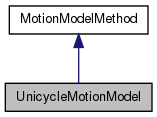
\includegraphics[width=190pt]{class_unicycle_motion_model__inherit__graph}
\end{center}
\end{figure}


\-Collaboration diagram for \-Unicycle\-Motion\-Model\-:
\nopagebreak
\begin{figure}[H]
\begin{center}
\leavevmode
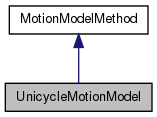
\includegraphics[width=190pt]{class_unicycle_motion_model__coll__graph}
\end{center}
\end{figure}
\subsection*{\-Public \-Types}
\begin{DoxyCompactItemize}
\item 
\hypertarget{class_unicycle_motion_model_add1e93839ad31a6b054551b31c6747ea}{typedef \*
\-Motion\-Model\-Method\-::\-Control\-Type {\bfseries \-Control\-Type}}\label{class_unicycle_motion_model_add1e93839ad31a6b054551b31c6747ea}

\item 
\hypertarget{class_unicycle_motion_model_a08ee5aeadfc71eaa00720bd56af71dfd}{typedef \*
\-Motion\-Model\-Method\-::\-Noise\-Type {\bfseries \-Noise\-Type}}\label{class_unicycle_motion_model_a08ee5aeadfc71eaa00720bd56af71dfd}

\item 
\hypertarget{class_unicycle_motion_model_aa7338364013e6001f926aa2a77f41df6}{typedef \*
\-Motion\-Model\-Method\-::\-Jacobian\-Type {\bfseries \-Jacobian\-Type}}\label{class_unicycle_motion_model_aa7338364013e6001f926aa2a77f41df6}

\end{DoxyCompactItemize}
\subsection*{\-Public \-Member \-Functions}
\begin{DoxyCompactItemize}
\item 
\hypertarget{class_unicycle_motion_model_a7d3d2725d5ae1167921005054c45a6c0}{{\bfseries \-Unicycle\-Motion\-Model} (const ompl\-::control\-::\-Space\-Information\-Ptr si, const char $\ast$path\-To\-Setup\-File)}\label{class_unicycle_motion_model_a7d3d2725d5ae1167921005054c45a6c0}

\item 
\hypertarget{class_unicycle_motion_model_ab5a56555b6b489cc3040fb61c71b5f15}{\hyperlink{class_unicycle_motion_model_ab5a56555b6b489cc3040fb61c71b5f15}{$\sim$\-Unicycle\-Motion\-Model} ()}\label{class_unicycle_motion_model_ab5a56555b6b489cc3040fb61c71b5f15}

\begin{DoxyCompactList}\small\item\em \-Destructor. \end{DoxyCompactList}\item 
\hypertarget{class_unicycle_motion_model_a7d78a6e7de4ad59dbd8aa0e6fd338ca7}{void \hyperlink{class_unicycle_motion_model_a7d78a6e7de4ad59dbd8aa0e6fd338ca7}{\-Evolve} (const ompl\-::base\-::\-State $\ast$state, const ompl\-::control\-::\-Control $\ast$control, const \-Noise\-Type \&w, ompl\-::base\-::\-State $\ast$result)}\label{class_unicycle_motion_model_a7d78a6e7de4ad59dbd8aa0e6fd338ca7}

\begin{DoxyCompactList}\small\item\em \-Propagate the system to the next state, given the current state, a control and a noise. \end{DoxyCompactList}\item 
\hypertarget{class_unicycle_motion_model_adf6f10302c29b5a196628af789e80739}{void \hyperlink{class_unicycle_motion_model_adf6f10302c29b5a196628af789e80739}{generate\-Open\-Loop\-Controls} (const ompl\-::base\-::\-State $\ast$start\-State, const ompl\-::base\-::\-State $\ast$end\-State, std\-::vector$<$ ompl\-::control\-::\-Control $\ast$ $>$ \&open\-Loop\-Controls)}\label{class_unicycle_motion_model_adf6f10302c29b5a196628af789e80739}

\begin{DoxyCompactList}\small\item\em \-Generate open loop control that drives robot from start to end state. \end{DoxyCompactList}\item 
\hypertarget{class_unicycle_motion_model_aff0d7239670e191b7d6ac518952b0428}{\-Noise\-Type \hyperlink{class_unicycle_motion_model_aff0d7239670e191b7d6ac518952b0428}{generate\-Noise} (const ompl\-::base\-::\-State $\ast$state, const ompl\-::control\-::\-Control $\ast$control)}\label{class_unicycle_motion_model_aff0d7239670e191b7d6ac518952b0428}

\begin{DoxyCompactList}\small\item\em \-Generate noise according to specified state and control input. \end{DoxyCompactList}\item 
\hypertarget{class_unicycle_motion_model_adb849fef38055401851adf4e87e8ec23}{\-Jacobian\-Type \hyperlink{class_unicycle_motion_model_adb849fef38055401851adf4e87e8ec23}{get\-State\-Jacobian} (const ompl\-::base\-::\-State $\ast$state, const ompl\-::control\-::\-Control $\ast$control, const \-Noise\-Type \&w)}\label{class_unicycle_motion_model_adb849fef38055401851adf4e87e8ec23}

\begin{DoxyCompactList}\small\item\em \-Calculate the state transition \-Jacobian i.\-e. df/dx where f is the transition function and x is the state. \end{DoxyCompactList}\item 
\hypertarget{class_unicycle_motion_model_a422cbf49ce1b509e7f031008483bd6ff}{\-Jacobian\-Type \hyperlink{class_unicycle_motion_model_a422cbf49ce1b509e7f031008483bd6ff}{get\-Control\-Jacobian} (const ompl\-::base\-::\-State $\ast$state, const ompl\-::control\-::\-Control $\ast$control, const \-Noise\-Type \&w)}\label{class_unicycle_motion_model_a422cbf49ce1b509e7f031008483bd6ff}

\begin{DoxyCompactList}\small\item\em \-Calculate the control transition \-Jacobian i.\-e. df/du where f is the transition function and u is the control. \end{DoxyCompactList}\item 
\hypertarget{class_unicycle_motion_model_a62aa73b58447613c0745dab9453760b7}{\-Jacobian\-Type \hyperlink{class_unicycle_motion_model_a62aa73b58447613c0745dab9453760b7}{get\-Noise\-Jacobian} (const ompl\-::base\-::\-State $\ast$state, const ompl\-::control\-::\-Control $\ast$control, const \-Noise\-Type \&w)}\label{class_unicycle_motion_model_a62aa73b58447613c0745dab9453760b7}

\begin{DoxyCompactList}\small\item\em \-Calculate the noise transition \-Jacobian i.\-e. df/dw where f is the transition function and w is the noise. \end{DoxyCompactList}\item 
\hypertarget{class_unicycle_motion_model_a1ae47461abed522cc1d611a1f60b6f7c}{arma\-::mat \hyperlink{class_unicycle_motion_model_a1ae47461abed522cc1d611a1f60b6f7c}{process\-Noise\-Covariance} (const ompl\-::base\-::\-State $\ast$state, const ompl\-::control\-::\-Control $\ast$control)}\label{class_unicycle_motion_model_a1ae47461abed522cc1d611a1f60b6f7c}

\begin{DoxyCompactList}\small\item\em \-Calculate the process noise covariance. \end{DoxyCompactList}\end{DoxyCompactItemize}
\subsection*{\-Private \-Member \-Functions}
\begin{DoxyCompactItemize}
\item 
\hypertarget{class_unicycle_motion_model_acb8c6afd05d931f53d8bb7b30184b83e}{arma\-::mat \hyperlink{class_unicycle_motion_model_acb8c6afd05d931f53d8bb7b30184b83e}{control\-Noise\-Covariance} (const ompl\-::control\-::\-Control $\ast$control)}\label{class_unicycle_motion_model_acb8c6afd05d931f53d8bb7b30184b83e}

\begin{DoxyCompactList}\small\item\em \-Generate the control noise covariance. \end{DoxyCompactList}\item 
\hypertarget{class_unicycle_motion_model_ae932dca27f26105c4d91e809b304b58d}{void \hyperlink{class_unicycle_motion_model_ae932dca27f26105c4d91e809b304b58d}{load\-Parameters} (const char $\ast$path\-To\-Setup\-File)}\label{class_unicycle_motion_model_ae932dca27f26105c4d91e809b304b58d}

\begin{DoxyCompactList}\small\item\em \-Load parameters from \-X\-M\-L. \end{DoxyCompactList}\end{DoxyCompactItemize}
\subsection*{\-Private \-Attributes}
\begin{DoxyCompactItemize}
\item 
\hypertarget{class_unicycle_motion_model_a8d47c96b281d68b16bfed5c6019b7502}{arma\-::colvec \hyperlink{class_unicycle_motion_model_a8d47c96b281d68b16bfed5c6019b7502}{sigma\-\_\-}}\label{class_unicycle_motion_model_a8d47c96b281d68b16bfed5c6019b7502}

\begin{DoxyCompactList}\small\item\em \-Bias standard deviation of the motion noise. \end{DoxyCompactList}\item 
\hypertarget{class_unicycle_motion_model_a4025caf061ba4e6426af86ae7074b7a9}{arma\-::colvec \hyperlink{class_unicycle_motion_model_a4025caf061ba4e6426af86ae7074b7a9}{eta\-\_\-}}\label{class_unicycle_motion_model_a4025caf061ba4e6426af86ae7074b7a9}

\begin{DoxyCompactList}\small\item\em \-Proportional standard deviation of the motion noise. \end{DoxyCompactList}\item 
\hypertarget{class_unicycle_motion_model_aa23aec795c0d97c5c54db925cfa27426}{arma\-::mat \hyperlink{class_unicycle_motion_model_aa23aec795c0d97c5c54db925cfa27426}{\-P\-\_\-\-Wg\-\_\-}}\label{class_unicycle_motion_model_aa23aec795c0d97c5c54db925cfa27426}

\begin{DoxyCompactList}\small\item\em \-Covariance of state additive noise. \end{DoxyCompactList}\item 
\hypertarget{class_unicycle_motion_model_a64f132a45af955098864992fd06e6bf0}{double \hyperlink{class_unicycle_motion_model_a64f132a45af955098864992fd06e6bf0}{max\-Angular\-Velocity\-\_\-}}\label{class_unicycle_motion_model_a64f132a45af955098864992fd06e6bf0}

\begin{DoxyCompactList}\small\item\em max rotational velocity \end{DoxyCompactList}\item 
\hypertarget{class_unicycle_motion_model_aaa92675e5a2f14a45ba08b6e008fd0b0}{double \hyperlink{class_unicycle_motion_model_aaa92675e5a2f14a45ba08b6e008fd0b0}{max\-Linear\-Velocity\-\_\-}}\label{class_unicycle_motion_model_aaa92675e5a2f14a45ba08b6e008fd0b0}

\begin{DoxyCompactList}\small\item\em max translational velocity \end{DoxyCompactList}\item 
\hypertarget{class_unicycle_motion_model_a35645b20aa08d05a106d9698ccc71919}{double \hyperlink{class_unicycle_motion_model_a35645b20aa08d05a106d9698ccc71919}{orbit\-Radius\-\_\-}}\label{class_unicycle_motion_model_a35645b20aa08d05a106d9698ccc71919}

\begin{DoxyCompactList}\small\item\em max translational velocity \end{DoxyCompactList}\item 
\hypertarget{class_unicycle_motion_model_a0e1c9df0b9f1736a92bf10bcf5ad597f}{double \hyperlink{class_unicycle_motion_model_a0e1c9df0b9f1736a92bf10bcf5ad597f}{min\-Linear\-Velocity\-\_\-}}\label{class_unicycle_motion_model_a0e1c9df0b9f1736a92bf10bcf5ad597f}

\begin{DoxyCompactList}\small\item\em min translational velocity \end{DoxyCompactList}\end{DoxyCompactItemize}
\subsection*{\-Static \-Private \-Attributes}
\begin{DoxyCompactItemize}
\item 
\hypertarget{class_unicycle_motion_model_a419ce60de8ab632ca7a77e80c8c3cdfa}{static const int {\bfseries state\-Dim} = 3}\label{class_unicycle_motion_model_a419ce60de8ab632ca7a77e80c8c3cdfa}

\item 
\hypertarget{class_unicycle_motion_model_a1902c45c50d76f9ccdc50f605ef29540}{static const int {\bfseries control\-Dim} = 2}\label{class_unicycle_motion_model_a1902c45c50d76f9ccdc50f605ef29540}

\item 
\hypertarget{class_unicycle_motion_model_a7bea8e301903e72bb5bc7d8c953f1681}{static const int {\bfseries motion\-Noise\-Dim} = 5}\label{class_unicycle_motion_model_a7bea8e301903e72bb5bc7d8c953f1681}

\end{DoxyCompactItemize}


\-The documentation for this class was generated from the following files\-:\begin{DoxyCompactItemize}
\item 
include/\-Motion\-Models/\-Unicycle\-Motion\-Model.\-h\item 
src/\-Motion\-Models/\-Unicycle\-Motion\-Model.\-cpp\end{DoxyCompactItemize}

\hypertarget{class_unicycle_state_propagator}{\section{\-Unicycle\-State\-Propagator \-Class \-Reference}
\label{class_unicycle_state_propagator}\index{\-Unicycle\-State\-Propagator@{\-Unicycle\-State\-Propagator}}
}


\-State propagation for a unicycle motion model.  




{\ttfamily \#include $<$\-Unicycle\-State\-Propagator.\-h$>$}

\subsection*{\-Public \-Member \-Functions}
\begin{DoxyCompactItemize}
\item 
\hypertarget{class_unicycle_state_propagator_a9b1d547c131b9a95ec25b01ab9f77fa1}{\hyperlink{class_unicycle_state_propagator_a9b1d547c131b9a95ec25b01ab9f77fa1}{\-Unicycle\-State\-Propagator} (const ompl\-::control\-::\-Space\-Information\-Ptr \&si)}\label{class_unicycle_state_propagator_a9b1d547c131b9a95ec25b01ab9f77fa1}

\begin{DoxyCompactList}\small\item\em \-Construct representation of a unicycle state propagator. \end{DoxyCompactList}\item 
\hypertarget{class_unicycle_state_propagator_a7cfd8b23df04636daacc5a21162ea950}{virtual bool \hyperlink{class_unicycle_state_propagator_a7cfd8b23df04636daacc5a21162ea950}{can\-Propagate\-Backward} (void) const }\label{class_unicycle_state_propagator_a7cfd8b23df04636daacc5a21162ea950}

\begin{DoxyCompactList}\small\item\em \-Will always return false, as the simulation can only proceed forward in time. \end{DoxyCompactList}\item 
virtual void \hyperlink{class_unicycle_state_propagator_a8fd2854e51c8dc14ba21e40e45b14736}{propagate} (const ompl\-::base\-::\-State $\ast$state, const ompl\-::control\-::\-Control $\ast$control, const double duration, ompl\-::base\-::\-State $\ast$result) const 
\begin{DoxyCompactList}\small\item\em \-Propagate from a state, under a given control, for some specified amount of time. \-We use the motion model to do the actual number crunching. \end{DoxyCompactList}\end{DoxyCompactItemize}
\subsection*{\-Protected \-Attributes}
\begin{DoxyCompactItemize}
\item 
\hypertarget{class_unicycle_state_propagator_aa7d52a6fb2ede1797badb5d6654061a3}{\-Motion\-Model\-Method\-::\-Motion\-Model\-Pointer {\bfseries motion\-Model\-\_\-}}\label{class_unicycle_state_propagator_aa7d52a6fb2ede1797badb5d6654061a3}

\end{DoxyCompactItemize}


\subsection{\-Detailed \-Description}
\-State propagation for a unicycle motion model. 



\subsection{\-Member \-Function \-Documentation}
\hypertarget{class_unicycle_state_propagator_a8fd2854e51c8dc14ba21e40e45b14736}{\index{\-Unicycle\-State\-Propagator@{\-Unicycle\-State\-Propagator}!propagate@{propagate}}
\index{propagate@{propagate}!UnicycleStatePropagator@{\-Unicycle\-State\-Propagator}}
\subsubsection[{propagate}]{\setlength{\rightskip}{0pt plus 5cm}void {\bf \-Unicycle\-State\-Propagator\-::propagate} (
\begin{DoxyParamCaption}
\item[{const ompl\-::base\-::\-State $\ast$}]{state, }
\item[{const ompl\-::control\-::\-Control $\ast$}]{control, }
\item[{const double}]{duration, }
\item[{ompl\-::base\-::\-State $\ast$}]{result}
\end{DoxyParamCaption}
) const\hspace{0.3cm}{\ttfamily  \mbox{[}virtual\mbox{]}}}}\label{class_unicycle_state_propagator_a8fd2854e51c8dc14ba21e40e45b14736}


\-Propagate from a state, under a given control, for some specified amount of time. \-We use the motion model to do the actual number crunching. 



\-The documentation for this class was generated from the following files\-:\begin{DoxyCompactItemize}
\item 
include/\-Motion\-Models/\-Unicycle\-State\-Propagator.\-h\item 
src/\-Motion\-Models/\-Unicycle\-State\-Propagator.\-cpp\end{DoxyCompactItemize}

\hypertarget{class_uniform_valid_belief_sampler}{\section{\-Uniform\-Valid\-Belief\-Sampler \-Class \-Reference}
\label{class_uniform_valid_belief_sampler}\index{\-Uniform\-Valid\-Belief\-Sampler@{\-Uniform\-Valid\-Belief\-Sampler}}
}


\-Generate valid samples using the \-Uniform sampling strategy.  




{\ttfamily \#include $<$\-Uniform\-Valid\-Belief\-Sampler.\-h$>$}

\subsection*{\-Public \-Member \-Functions}
\begin{DoxyCompactItemize}
\item 
\hypertarget{class_uniform_valid_belief_sampler_a5c05246571e95d2a631679b57431232a}{\hyperlink{class_uniform_valid_belief_sampler_a5c05246571e95d2a631679b57431232a}{\-Uniform\-Valid\-Belief\-Sampler} (const \hyperlink{classfirm_1_1_space_information}{firm\-::\-Space\-Information} $\ast$si)}\label{class_uniform_valid_belief_sampler_a5c05246571e95d2a631679b57431232a}

\begin{DoxyCompactList}\small\item\em \-Constructor. \end{DoxyCompactList}\item 
\hypertarget{class_uniform_valid_belief_sampler_ad2cd6ccdd48289255ee92b919ce68982}{virtual bool {\bfseries sample} (\-State $\ast$state)}\label{class_uniform_valid_belief_sampler_ad2cd6ccdd48289255ee92b919ce68982}

\item 
\hypertarget{class_uniform_valid_belief_sampler_a59da95b1d779e781149e3b83919f5684}{virtual bool {\bfseries sample\-Near} (\-State $\ast$state, const \-State $\ast$near, const double distance)}\label{class_uniform_valid_belief_sampler_a59da95b1d779e781149e3b83919f5684}

\end{DoxyCompactItemize}
\subsection*{\-Protected \-Member \-Functions}
\begin{DoxyCompactItemize}
\item 
bool \hyperlink{class_uniform_valid_belief_sampler_acb6c744f26fe0c07b959d2329aed90eb}{is\-Observable} (ompl\-::base\-::\-State $\ast$state)
\end{DoxyCompactItemize}
\subsection*{\-Protected \-Attributes}
\begin{DoxyCompactItemize}
\item 
\-State\-Sampler\-Ptr \hyperlink{class_uniform_valid_belief_sampler_a1d133b2161245e32544833d5be54e595}{sampler\-\_\-}
\begin{DoxyCompactList}\small\item\em \-The sampler to build upon. \end{DoxyCompactList}\end{DoxyCompactItemize}


\subsection{\-Detailed \-Description}
\-Generate valid samples using the \-Uniform sampling strategy. 

\subsection{\-Member \-Function \-Documentation}
\hypertarget{class_uniform_valid_belief_sampler_acb6c744f26fe0c07b959d2329aed90eb}{\index{\-Uniform\-Valid\-Belief\-Sampler@{\-Uniform\-Valid\-Belief\-Sampler}!is\-Observable@{is\-Observable}}
\index{is\-Observable@{is\-Observable}!UniformValidBeliefSampler@{\-Uniform\-Valid\-Belief\-Sampler}}
\subsubsection[{is\-Observable}]{\setlength{\rightskip}{0pt plus 5cm}bool {\bf \-Uniform\-Valid\-Belief\-Sampler\-::is\-Observable} (
\begin{DoxyParamCaption}
\item[{ompl\-::base\-::\-State $\ast$}]{state}
\end{DoxyParamCaption}
)\hspace{0.3cm}{\ttfamily  \mbox{[}protected\mbox{]}}}}\label{class_uniform_valid_belief_sampler_acb6c744f26fe0c07b959d2329aed90eb}
brief \-Checks if the sample is observable i.\-e. \-If it can observe sufficient landmarks \-Ideally, observability check should be performed in the filter instead of obs model 

\subsection{\-Member \-Data \-Documentation}
\hypertarget{class_uniform_valid_belief_sampler_a1d133b2161245e32544833d5be54e595}{\index{\-Uniform\-Valid\-Belief\-Sampler@{\-Uniform\-Valid\-Belief\-Sampler}!sampler\-\_\-@{sampler\-\_\-}}
\index{sampler\-\_\-@{sampler\-\_\-}!UniformValidBeliefSampler@{\-Uniform\-Valid\-Belief\-Sampler}}
\subsubsection[{sampler\-\_\-}]{\setlength{\rightskip}{0pt plus 5cm}\-State\-Sampler\-Ptr {\bf \-Uniform\-Valid\-Belief\-Sampler\-::sampler\-\_\-}\hspace{0.3cm}{\ttfamily  \mbox{[}protected\mbox{]}}}}\label{class_uniform_valid_belief_sampler_a1d133b2161245e32544833d5be54e595}


\-The sampler to build upon. 

void set\-Observation\-Model(\-Observation\-Model\-Pointer om) \{ observation\-Model\-\_\- = om; \} 

\-The documentation for this class was generated from the following files\-:\begin{DoxyCompactItemize}
\item 
include/\-Samplers/\-Uniform\-Valid\-Belief\-Sampler.\-h\item 
src/\-Samplers/\-Uniform\-Valid\-Belief\-Sampler.\-cpp\end{DoxyCompactItemize}

\hypertarget{struct_f_i_r_m_1_1vertex__flags__t}{\section{\-F\-I\-R\-M\-:\-:vertex\-\_\-flags\-\_\-t \-Struct \-Reference}
\label{struct_f_i_r_m_1_1vertex__flags__t}\index{\-F\-I\-R\-M\-::vertex\-\_\-flags\-\_\-t@{\-F\-I\-R\-M\-::vertex\-\_\-flags\-\_\-t}}
}
\subsection*{\-Public \-Types}
\begin{DoxyCompactItemize}
\item 
\hypertarget{struct_f_i_r_m_1_1vertex__flags__t_ac76c9256a586ee6d6f9253ada4929e13}{typedef boost\-::vertex\-\_\-property\-\_\-tag {\bfseries kind}}\label{struct_f_i_r_m_1_1vertex__flags__t_ac76c9256a586ee6d6f9253ada4929e13}

\end{DoxyCompactItemize}


\-The documentation for this struct was generated from the following file\-:\begin{DoxyCompactItemize}
\item 
include/\-Planner/\-F\-I\-R\-M.\-h\end{DoxyCompactItemize}

\hypertarget{struct_f_i_r_m_1_1vertex__state__t}{\section{\-F\-I\-R\-M\-:\-:vertex\-\_\-state\-\_\-t \-Struct \-Reference}
\label{struct_f_i_r_m_1_1vertex__state__t}\index{\-F\-I\-R\-M\-::vertex\-\_\-state\-\_\-t@{\-F\-I\-R\-M\-::vertex\-\_\-state\-\_\-t}}
}
\subsection*{\-Public \-Types}
\begin{DoxyCompactItemize}
\item 
\hypertarget{struct_f_i_r_m_1_1vertex__state__t_a1917aebbc6fd5d22c666bb6400546c15}{typedef boost\-::vertex\-\_\-property\-\_\-tag {\bfseries kind}}\label{struct_f_i_r_m_1_1vertex__state__t_a1917aebbc6fd5d22c666bb6400546c15}

\end{DoxyCompactItemize}


\-The documentation for this struct was generated from the following file\-:\begin{DoxyCompactItemize}
\item 
include/\-Planner/\-F\-I\-R\-M.\-h\end{DoxyCompactItemize}

\hypertarget{struct_f_i_r_m_1_1vertex__successful__connection__attempts__t}{\section{\-F\-I\-R\-M\-:\-:vertex\-\_\-successful\-\_\-connection\-\_\-attempts\-\_\-t \-Struct \-Reference}
\label{struct_f_i_r_m_1_1vertex__successful__connection__attempts__t}\index{\-F\-I\-R\-M\-::vertex\-\_\-successful\-\_\-connection\-\_\-attempts\-\_\-t@{\-F\-I\-R\-M\-::vertex\-\_\-successful\-\_\-connection\-\_\-attempts\-\_\-t}}
}
\subsection*{\-Public \-Types}
\begin{DoxyCompactItemize}
\item 
\hypertarget{struct_f_i_r_m_1_1vertex__successful__connection__attempts__t_a733ba6f888f1adc641d746377eb13eec}{typedef boost\-::vertex\-\_\-property\-\_\-tag {\bfseries kind}}\label{struct_f_i_r_m_1_1vertex__successful__connection__attempts__t_a733ba6f888f1adc641d746377eb13eec}

\item 
\hypertarget{struct_f_i_r_m_1_1vertex__successful__connection__attempts__t_a733ba6f888f1adc641d746377eb13eec}{typedef boost\-::vertex\-\_\-property\-\_\-tag {\bfseries kind}}\label{struct_f_i_r_m_1_1vertex__successful__connection__attempts__t_a733ba6f888f1adc641d746377eb13eec}

\item 
\hypertarget{struct_f_i_r_m_1_1vertex__successful__connection__attempts__t_a733ba6f888f1adc641d746377eb13eec}{typedef boost\-::vertex\-\_\-property\-\_\-tag {\bfseries kind}}\label{struct_f_i_r_m_1_1vertex__successful__connection__attempts__t_a733ba6f888f1adc641d746377eb13eec}

\end{DoxyCompactItemize}


\-The documentation for this struct was generated from the following files\-:\begin{DoxyCompactItemize}
\item 
include/\-Planner/\-F\-I\-R\-M-\/old-\/v2.\-h\item 
include/\-Planner/\-F\-I\-R\-M-\/old.\-h\item 
include/\-Planner/\-F\-I\-R\-M.\-h\end{DoxyCompactItemize}

\hypertarget{struct_f_i_r_m_1_1vertex__total__connection__attempts__t}{\section{\-F\-I\-R\-M\-:\-:vertex\-\_\-total\-\_\-connection\-\_\-attempts\-\_\-t \-Struct \-Reference}
\label{struct_f_i_r_m_1_1vertex__total__connection__attempts__t}\index{\-F\-I\-R\-M\-::vertex\-\_\-total\-\_\-connection\-\_\-attempts\-\_\-t@{\-F\-I\-R\-M\-::vertex\-\_\-total\-\_\-connection\-\_\-attempts\-\_\-t}}
}
\subsection*{\-Public \-Types}
\begin{DoxyCompactItemize}
\item 
\hypertarget{struct_f_i_r_m_1_1vertex__total__connection__attempts__t_afb2aba317a24c9d5032e85713f69f8d0}{typedef boost\-::vertex\-\_\-property\-\_\-tag {\bfseries kind}}\label{struct_f_i_r_m_1_1vertex__total__connection__attempts__t_afb2aba317a24c9d5032e85713f69f8d0}

\end{DoxyCompactItemize}


\-The documentation for this struct was generated from the following file\-:\begin{DoxyCompactItemize}
\item 
include/\-Planner/\-F\-I\-R\-M.\-h\end{DoxyCompactItemize}

\hypertarget{class_visualizer}{\section{Visualizer Class Reference}
\label{class_visualizer}\index{Visualizer@{Visualizer}}
}
\subsection*{Classes}
\begin{DoxyCompactItemize}
\item 
struct \hyperlink{struct_visualizer_1_1_v_z_r_feedback_edge}{V\-Z\-R\-Feedback\-Edge}
\end{DoxyCompactItemize}
\subsection*{Public Types}
\begin{DoxyCompactItemize}
\item 
enum \hyperlink{class_visualizer_a2710d7bdd6700c034876a3c43c328cd7}{V\-Z\-R\-State\-Type} \{ {\bfseries True\-State}, 
{\bfseries Belief\-State}, 
{\bfseries Graph\-Node\-State}
 \}
\begin{DoxyCompactList}\small\item\em Helps distinguish between states while drawing. \end{DoxyCompactList}\item 
enum {\bfseries V\-Z\-R\-Drawing\-Mode} \{ \\*
{\bfseries Node\-View\-Mode}, 
{\bfseries Feedback\-View\-Mode}, 
{\bfseries P\-R\-M\-View\-Mode}, 
{\bfseries Rollout\-Mode}, 
\\*
{\bfseries Multi\-Modal\-Mode}
 \}
\end{DoxyCompactItemize}
\subsection*{Static Public Member Functions}
\begin{DoxyCompactItemize}
\item 
\hypertarget{class_visualizer_af1d495ef8b48411cac724f242347b541}{static void \hyperlink{class_visualizer_af1d495ef8b48411cac724f242347b541}{add\-Landmarks} (const std\-::vector$<$ arma\-::colvec $>$ \&landmarks)}\label{class_visualizer_af1d495ef8b48411cac724f242347b541}

\begin{DoxyCompactList}\small\item\em Add the landmarks in the environment. \end{DoxyCompactList}\item 
\hypertarget{class_visualizer_a6c7ac8469193d405c73ed8d2edd5bc63}{static void \hyperlink{class_visualizer_a6c7ac8469193d405c73ed8d2edd5bc63}{add\-State} (ompl\-::base\-::\-State $\ast$state)}\label{class_visualizer_a6c7ac8469193d405c73ed8d2edd5bc63}

\begin{DoxyCompactList}\small\item\em Add the states i.\-e. graph nodes to be drawn. \end{DoxyCompactList}\item 
\hypertarget{class_visualizer_a05802a504ef9a4804af730d2848b9689}{static void \hyperlink{class_visualizer_a05802a504ef9a4804af730d2848b9689}{clear\-States} ()}\label{class_visualizer_a05802a504ef9a4804af730d2848b9689}

\begin{DoxyCompactList}\small\item\em Clear the state container. \end{DoxyCompactList}\item 
\hypertarget{class_visualizer_a19a65a5d08ade114252d809b78976b1f}{static void \hyperlink{class_visualizer_a19a65a5d08ade114252d809b78976b1f}{add\-Belief\-Mode} (ompl\-::base\-::\-State $\ast$state)}\label{class_visualizer_a19a65a5d08ade114252d809b78976b1f}

\begin{DoxyCompactList}\small\item\em Add state to belief mode list. \end{DoxyCompactList}\item 
\hypertarget{class_visualizer_a9bf180935f50440ed3ab68602f32f78a}{static void \hyperlink{class_visualizer_a9bf180935f50440ed3ab68602f32f78a}{clear\-Belief\-Modes} ()}\label{class_visualizer_a9bf180935f50440ed3ab68602f32f78a}

\begin{DoxyCompactList}\small\item\em Clear belief Modes. \end{DoxyCompactList}\item 
\hypertarget{class_visualizer_a31ce4b4a4865921d5c8d72b94f6dd7a5}{static void \hyperlink{class_visualizer_a31ce4b4a4865921d5c8d72b94f6dd7a5}{add\-Graph\-Edge} (const ompl\-::base\-::\-State $\ast$source, const ompl\-::base\-::\-State $\ast$target)}\label{class_visualizer_a31ce4b4a4865921d5c8d72b94f6dd7a5}

\begin{DoxyCompactList}\small\item\em Add a Roadmap Graph edge to the visualization. \end{DoxyCompactList}\item 
\hypertarget{class_visualizer_a728bc4cf562902c5ba4a79aed4685875}{static void {\bfseries add\-Feedback\-Edge} (const ompl\-::base\-::\-State $\ast$source, const ompl\-::base\-::\-State $\ast$target, double cost)}\label{class_visualizer_a728bc4cf562902c5ba4a79aed4685875}

\item 
\hypertarget{class_visualizer_a207b9cdfc68a6d327ba04bd5d6b5e94e}{static void \hyperlink{class_visualizer_a207b9cdfc68a6d327ba04bd5d6b5e94e}{add\-Rollout\-Connection} (const ompl\-::base\-::\-State $\ast$source, const ompl\-::base\-::\-State $\ast$target)}\label{class_visualizer_a207b9cdfc68a6d327ba04bd5d6b5e94e}

\begin{DoxyCompactList}\small\item\em Add a rollout connection to the visualization. \end{DoxyCompactList}\item 
\hypertarget{class_visualizer_a364f1254d282cad1717ca9ad0c4b4081}{static void \hyperlink{class_visualizer_a364f1254d282cad1717ca9ad0c4b4081}{add\-Most\-Likely\-Path\-Edge} (const ompl\-::base\-::\-State $\ast$source, const ompl\-::base\-::\-State $\ast$target)}\label{class_visualizer_a364f1254d282cad1717ca9ad0c4b4081}

\begin{DoxyCompactList}\small\item\em Add a rollout connection to the visualization. \end{DoxyCompactList}\item 
\hypertarget{class_visualizer_a474b9dd973d8b1b490b33587ad9aa86d}{static void {\bfseries set\-Chosen\-Rollout\-Connection} (const ompl\-::base\-::\-State $\ast$source, const ompl\-::base\-::\-State $\ast$target)}\label{class_visualizer_a474b9dd973d8b1b490b33587ad9aa86d}

\item 
\hypertarget{class_visualizer_a918f5598cf7479d190f8d29600fa16d5}{static void {\bfseries draw\-Robot\-Path} ()}\label{class_visualizer_a918f5598cf7479d190f8d29600fa16d5}

\item 
\hypertarget{class_visualizer_a652f193100d7d75a85061d170b6e4a5d}{static void {\bfseries set\-Mode} (V\-Z\-R\-Drawing\-Mode mode)}\label{class_visualizer_a652f193100d7d75a85061d170b6e4a5d}

\item 
\hypertarget{class_visualizer_a7ee82eedc8128237b09d8eefaf421679}{static void {\bfseries Clear\-Feedback\-Edges} ()}\label{class_visualizer_a7ee82eedc8128237b09d8eefaf421679}

\item 
\hypertarget{class_visualizer_ada63070c0f48730528ae11fe6116cb89}{static void {\bfseries clear\-Rollout\-Connections} ()}\label{class_visualizer_ada63070c0f48730528ae11fe6116cb89}

\item 
\hypertarget{class_visualizer_a9f2be28abd54f00462af50b1cac3a135}{static void {\bfseries clear\-Most\-Likely\-Path} ()}\label{class_visualizer_a9f2be28abd54f00462af50b1cac3a135}

\item 
\hypertarget{class_visualizer_afc6c18807bedf44057734905cef8e550}{static void {\bfseries add\-Open\-Loop\-R\-R\-T\-Path} (const ompl\-::geometric\-::\-Path\-Geometric path)}\label{class_visualizer_afc6c18807bedf44057734905cef8e550}

\item 
\hypertarget{class_visualizer_aae26a006f1d085045429c21649d96d8b}{static void {\bfseries clear\-Open\-Loop\-R\-R\-T\-Paths} ()}\label{class_visualizer_aae26a006f1d085045429c21649d96d8b}

\item 
\hypertarget{class_visualizer_a65c3c5451f614eda7d0ed83613ad1ed4}{static void \hyperlink{class_visualizer_a65c3c5451f614eda7d0ed83613ad1ed4}{update\-True\-State} (const ompl\-::base\-::\-State $\ast$state)}\label{class_visualizer_a65c3c5451f614eda7d0ed83613ad1ed4}

\begin{DoxyCompactList}\small\item\em update the robot's true state for drawing \end{DoxyCompactList}\item 
\hypertarget{class_visualizer_a00b248fc1bc0bf1f445d1b72cbaad301}{static void \hyperlink{class_visualizer_a00b248fc1bc0bf1f445d1b72cbaad301}{update\-Current\-Belief} (const ompl\-::base\-::\-State $\ast$state)}\label{class_visualizer_a00b248fc1bc0bf1f445d1b72cbaad301}

\begin{DoxyCompactList}\small\item\em update the robot's belief for drawing \end{DoxyCompactList}\item 
\hypertarget{class_visualizer_a03f2c860d508cee10fdcf221fdfa8899}{static void \hyperlink{class_visualizer_a03f2c860d508cee10fdcf221fdfa8899}{update\-Space\-Information} (const firm\-::\-Space\-Information\-::\-Space\-Information\-Ptr si)}\label{class_visualizer_a03f2c860d508cee10fdcf221fdfa8899}

\begin{DoxyCompactList}\small\item\em Copy the space information pointer. \end{DoxyCompactList}\item 
\hypertarget{class_visualizer_acca6818239d3d2e8cabdfb7321e817b9}{static void {\bfseries update\-Renderer} (ompl\-::app\-::\-Render\-Geometry $\ast$renderer)}\label{class_visualizer_acca6818239d3d2e8cabdfb7321e817b9}

\item 
\hypertarget{class_visualizer_a3218c7fa2f83159188c624f04e982a24}{static void {\bfseries update\-Renderer} (const ompl\-::app\-::\-Rigid\-Body\-Geometry \&rbg, const ompl\-::app\-::\-Geometric\-State\-Extractor \&se)}\label{class_visualizer_a3218c7fa2f83159188c624f04e982a24}

\item 
\hypertarget{class_visualizer_abacab1d3c34cf91364ea0f45bc0f7473}{static void {\bfseries clear\-Robot\-Path} ()}\label{class_visualizer_abacab1d3c34cf91364ea0f45bc0f7473}

\item 
\hypertarget{class_visualizer_a2544a80a7ac2f432661f199e4cb08130}{static void \hyperlink{class_visualizer_a2544a80a7ac2f432661f199e4cb08130}{draw\-Landmark} (arma\-::colvec \&landmark)}\label{class_visualizer_a2544a80a7ac2f432661f199e4cb08130}

\begin{DoxyCompactList}\small\item\em Draw a single landmark that is passed to this function. \end{DoxyCompactList}\item 
\hypertarget{class_visualizer_a355fdbecb72d38f8a651c7dd75d1d6e1}{static void \hyperlink{class_visualizer_a355fdbecb72d38f8a651c7dd75d1d6e1}{draw\-Robot} (const ompl\-::base\-::\-State $\ast$state)}\label{class_visualizer_a355fdbecb72d38f8a651c7dd75d1d6e1}

\begin{DoxyCompactList}\small\item\em Draw the true robot rendering. \end{DoxyCompactList}\item 
\hypertarget{class_visualizer_ac4282cfa39ebe59311fee512d46cb9f7}{static void \hyperlink{class_visualizer_ac4282cfa39ebe59311fee512d46cb9f7}{draw\-State} (const ompl\-::base\-::\-State $\ast$state, \hyperlink{class_visualizer_a2710d7bdd6700c034876a3c43c328cd7}{V\-Z\-R\-State\-Type} state\-Type)}\label{class_visualizer_ac4282cfa39ebe59311fee512d46cb9f7}

\begin{DoxyCompactList}\small\item\em Draw a single state that is passed to this function. \end{DoxyCompactList}\item 
\hypertarget{class_visualizer_aca4b5a57dbd7d491b3889bd07cc04afa}{static void \hyperlink{class_visualizer_aca4b5a57dbd7d491b3889bd07cc04afa}{draw\-Edge} (const ompl\-::base\-::\-State $\ast$source, const ompl\-::base\-::\-State $\ast$target)}\label{class_visualizer_aca4b5a57dbd7d491b3889bd07cc04afa}

\begin{DoxyCompactList}\small\item\em Draw an edge that belongs to the Roadmap graph. \end{DoxyCompactList}\item 
\hypertarget{class_visualizer_a93168dcaa16bcb97a647d03183459778}{static void \hyperlink{class_visualizer_a93168dcaa16bcb97a647d03183459778}{draw\-Graph\-Belief\-Nodes} ()}\label{class_visualizer_a93168dcaa16bcb97a647d03183459778}

\begin{DoxyCompactList}\small\item\em Draw the stored graph nodes. \end{DoxyCompactList}\item 
\hypertarget{class_visualizer_a9755c745e5aeb4dc76b007594f95fd09}{static void \hyperlink{class_visualizer_a9755c745e5aeb4dc76b007594f95fd09}{draw\-Belief\-Modes} ()}\label{class_visualizer_a9755c745e5aeb4dc76b007594f95fd09}

\begin{DoxyCompactList}\small\item\em Draw belief modes. \end{DoxyCompactList}\item 
\hypertarget{class_visualizer_a12171ebc167f32a2a90c6e94d9505331}{static void \hyperlink{class_visualizer_a12171ebc167f32a2a90c6e94d9505331}{draw\-Graph\-Edges} ()}\label{class_visualizer_a12171ebc167f32a2a90c6e94d9505331}

\begin{DoxyCompactList}\small\item\em Draw the edges in the roadmap graph. \end{DoxyCompactList}\item 
\hypertarget{class_visualizer_ab484f66c1477eee940a90c436d320d1d}{static void \hyperlink{class_visualizer_ab484f66c1477eee940a90c436d320d1d}{draw\-Feedback\-Edges} ()}\label{class_visualizer_ab484f66c1477eee940a90c436d320d1d}

\begin{DoxyCompactList}\small\item\em Draw graph feedback edges. \end{DoxyCompactList}\item 
\hypertarget{class_visualizer_a3d9d939e1deef7f24c10d6ebbf794206}{static void \hyperlink{class_visualizer_a3d9d939e1deef7f24c10d6ebbf794206}{draw\-Rollout\-Connections} ()}\label{class_visualizer_a3d9d939e1deef7f24c10d6ebbf794206}

\begin{DoxyCompactList}\small\item\em Draw rollout connections. \end{DoxyCompactList}\item 
\hypertarget{class_visualizer_aae94674acda11f26522581791b310cb1}{static void \hyperlink{class_visualizer_aae94674acda11f26522581791b310cb1}{draw\-Most\-Likely\-Path} ()}\label{class_visualizer_aae94674acda11f26522581791b310cb1}

\begin{DoxyCompactList}\small\item\em Draw the most likely path under \hyperlink{class_f_i_r_m}{F\-I\-R\-M}. \end{DoxyCompactList}\item 
\hypertarget{class_visualizer_ada993e034ff9541d069d2e894ed51f5d}{static void \hyperlink{class_visualizer_ada993e034ff9541d069d2e894ed51f5d}{draw\-Environment} ()}\label{class_visualizer_ada993e034ff9541d069d2e894ed51f5d}

\begin{DoxyCompactList}\small\item\em Draw the X\&Y bounds. \end{DoxyCompactList}\item 
\hypertarget{class_visualizer_af4b7f35e3dff8daaf9cc79ac1f9140cd}{static void {\bfseries draw\-Obstacle} ()}\label{class_visualizer_af4b7f35e3dff8daaf9cc79ac1f9140cd}

\item 
\hypertarget{class_visualizer_a35dec37e9c258e2074f1b3ccf7e7a01c}{static void \hyperlink{class_visualizer_a35dec37e9c258e2074f1b3ccf7e7a01c}{draw\-Geometric\-Path} (const ompl\-::geometric\-::\-Path\-Geometric path)}\label{class_visualizer_a35dec37e9c258e2074f1b3ccf7e7a01c}

\begin{DoxyCompactList}\small\item\em Draw geometric path. \end{DoxyCompactList}\item 
\hypertarget{class_visualizer_a7e56ae25a51fe94ac158f33a0b29fba8}{static void {\bfseries draw\-Open\-Loop\-R\-R\-T\-Paths} ()}\label{class_visualizer_a7e56ae25a51fe94ac158f33a0b29fba8}

\item 
\hypertarget{class_visualizer_a5dc2040eeebd6568034c3230cccd8530}{static void \hyperlink{class_visualizer_a5dc2040eeebd6568034c3230cccd8530}{refresh} ()}\label{class_visualizer_a5dc2040eeebd6568034c3230cccd8530}

\begin{DoxyCompactList}\small\item\em Refresh the drawing and show latest scenario. \end{DoxyCompactList}\item 
\hypertarget{class_visualizer_a8a7b15c56dc6823af1cdbafdb238ba1a}{static bool {\bfseries save\-Video} ()}\label{class_visualizer_a8a7b15c56dc6823af1cdbafdb238ba1a}

\item 
\hypertarget{class_visualizer_a22e7426a0b03231d20a2e7ce37d728e7}{static void {\bfseries do\-Save\-Video} (bool flag)}\label{class_visualizer_a22e7426a0b03231d20a2e7ce37d728e7}

\end{DoxyCompactItemize}
\subsection*{Static Private Attributes}
\begin{DoxyCompactItemize}
\item 
\hypertarget{class_visualizer_ad6771691744b01cc232ea171e1e2a4ab}{static std\-::list\\*
$<$ ompl\-::base\-::\-State $\ast$ $>$ \hyperlink{class_visualizer_ad6771691744b01cc232ea171e1e2a4ab}{states\-\_\-}}\label{class_visualizer_ad6771691744b01cc232ea171e1e2a4ab}

\begin{DoxyCompactList}\small\item\em A list that stores the graph nodes. \end{DoxyCompactList}\item 
\hypertarget{class_visualizer_a7ca3a80de8106a9d53b8b25247aadc07}{static boost\-::mutex \hyperlink{class_visualizer_a7ca3a80de8106a9d53b8b25247aadc07}{draw\-Mutex\-\_\-}}\label{class_visualizer_a7ca3a80de8106a9d53b8b25247aadc07}

\begin{DoxyCompactList}\small\item\em visualizer thread mutex, allows us to place a lock so that class state changes while drawing \end{DoxyCompactList}\item 
\hypertarget{class_visualizer_a2a25f3b2372418e1088cd889f26df95d}{static ompl\-::base\-::\-State $\ast$ \hyperlink{class_visualizer_a2a25f3b2372418e1088cd889f26df95d}{true\-State\-\_\-}}\label{class_visualizer_a2a25f3b2372418e1088cd889f26df95d}

\begin{DoxyCompactList}\small\item\em Store the robots true state. \end{DoxyCompactList}\item 
\hypertarget{class_visualizer_a4f39505b9d7a4590ade4d87b1a9004d7}{static ompl\-::base\-::\-State $\ast$ \hyperlink{class_visualizer_a4f39505b9d7a4590ade4d87b1a9004d7}{current\-Belief\-\_\-}}\label{class_visualizer_a4f39505b9d7a4590ade4d87b1a9004d7}

\begin{DoxyCompactList}\small\item\em Store the robots belief state. \end{DoxyCompactList}\item 
\hypertarget{class_visualizer_a13a9427e5bbd1301b615bf81ed2bff99}{static std\-::list\\*
$<$ ompl\-::base\-::\-State $\ast$ $>$ \hyperlink{class_visualizer_a13a9427e5bbd1301b615bf81ed2bff99}{belief\-Modes\-\_\-}}\label{class_visualizer_a13a9427e5bbd1301b615bf81ed2bff99}

\begin{DoxyCompactList}\small\item\em Store the belief modes for multi-\/modal operation. \end{DoxyCompactList}\item 
\hypertarget{class_visualizer_a0cbfe1d4b50e562395c520fec568299d}{static std\-::vector$<$ arma\-::colvec $>$ \hyperlink{class_visualizer_a0cbfe1d4b50e562395c520fec568299d}{landmarks\-\_\-}}\label{class_visualizer_a0cbfe1d4b50e562395c520fec568299d}

\begin{DoxyCompactList}\small\item\em Store the landmarks. \end{DoxyCompactList}\item 
\hypertarget{class_visualizer_a111664b7b5b6a2c11e5bb3e3cb8fcd01}{static \\*
firm\-::\-Space\-Information\-::\-Space\-Information\-Ptr \hyperlink{class_visualizer_a111664b7b5b6a2c11e5bb3e3cb8fcd01}{si\-\_\-}}\label{class_visualizer_a111664b7b5b6a2c11e5bb3e3cb8fcd01}

\begin{DoxyCompactList}\small\item\em A pointer to the space information, because the visualizer must know what space its drawing. \end{DoxyCompactList}\item 
\hypertarget{class_visualizer_a2ff4816da3e84d1132ff0fafbdbadb98}{static std\-::vector$<$ std\-::pair\\*
$<$ const ompl\-::base\-::\-State \\*
$\ast$, const ompl\-::base\-::\-State $\ast$ $>$ $>$ \hyperlink{class_visualizer_a2ff4816da3e84d1132ff0fafbdbadb98}{graph\-Edges\-\_\-}}\label{class_visualizer_a2ff4816da3e84d1132ff0fafbdbadb98}

\begin{DoxyCompactList}\small\item\em Store the Roadmap graph edges. \end{DoxyCompactList}\item 
\hypertarget{class_visualizer_a9a3922205f833fd7a83e33a1501e0d74}{static std\-::vector$<$ std\-::pair\\*
$<$ const ompl\-::base\-::\-State \\*
$\ast$, const ompl\-::base\-::\-State $\ast$ $>$ $>$ \hyperlink{class_visualizer_a9a3922205f833fd7a83e33a1501e0d74}{rollout\-Connections\-\_\-}}\label{class_visualizer_a9a3922205f833fd7a83e33a1501e0d74}

\begin{DoxyCompactList}\small\item\em Store the Rollout connections. \end{DoxyCompactList}\item 
\hypertarget{class_visualizer_a67cb011e12b48a8aa95249324fd9ed87}{static std\-::vector$<$ std\-::pair\\*
$<$ const ompl\-::base\-::\-State \\*
$\ast$, const ompl\-::base\-::\-State $\ast$ $>$ $>$ \hyperlink{class_visualizer_a67cb011e12b48a8aa95249324fd9ed87}{most\-Likely\-Path\-\_\-}}\label{class_visualizer_a67cb011e12b48a8aa95249324fd9ed87}

\begin{DoxyCompactList}\small\item\em Store the Rollout connections. \end{DoxyCompactList}\item 
\hypertarget{class_visualizer_a241e08e6835a4655fb32b0171dcb9d53}{static boost\-::optional\\*
$<$ std\-::pair$<$ const \\*
ompl\-::base\-::\-State $\ast$, const \\*
ompl\-::base\-::\-State $\ast$ $>$ $>$ \hyperlink{class_visualizer_a241e08e6835a4655fb32b0171dcb9d53}{chosen\-Rollout\-Connection\-\_\-}}\label{class_visualizer_a241e08e6835a4655fb32b0171dcb9d53}

\begin{DoxyCompactList}\small\item\em The rollout connection that gets chosen as the next target. \end{DoxyCompactList}\item 
\hypertarget{class_visualizer_a506f4480f1c47d9105283ca07b600d64}{static std\-::vector\\*
$<$ \hyperlink{struct_visualizer_1_1_v_z_r_feedback_edge}{V\-Z\-R\-Feedback\-Edge} $>$ \hyperlink{class_visualizer_a506f4480f1c47d9105283ca07b600d64}{feedback\-Edges\-\_\-}}\label{class_visualizer_a506f4480f1c47d9105283ca07b600d64}

\begin{DoxyCompactList}\small\item\em Store the feedback edges. \end{DoxyCompactList}\item 
\hypertarget{class_visualizer_a887ebf260abf93bf1a88560faf7eccb2}{static std\-::vector$<$ const \\*
ompl\-::base\-::\-State $\ast$ $>$ \hyperlink{class_visualizer_a887ebf260abf93bf1a88560faf7eccb2}{robot\-Path\-\_\-}}\label{class_visualizer_a887ebf260abf93bf1a88560faf7eccb2}

\begin{DoxyCompactList}\small\item\em stores the sequence of states of the real robot \end{DoxyCompactList}\item 
\hypertarget{class_visualizer_a11d99288fa2898f177676f7f40ab52de}{static std\-::vector\\*
$<$ ompl\-::geometric\-::\-Path\-Geometric $>$ \hyperlink{class_visualizer_a11d99288fa2898f177676f7f40ab52de}{open\-Loop\-R\-R\-T\-Paths\-\_\-}}\label{class_visualizer_a11d99288fa2898f177676f7f40ab52de}

\begin{DoxyCompactList}\small\item\em Container for R\-R\-T paths generated as candidates during Multi-\/\-Modal operation. \end{DoxyCompactList}\item 
\hypertarget{class_visualizer_aa43c5908a3ae82a79c06d126fb32b505}{static V\-Z\-R\-Drawing\-Mode \hyperlink{class_visualizer_aa43c5908a3ae82a79c06d126fb32b505}{mode\-\_\-}}\label{class_visualizer_aa43c5908a3ae82a79c06d126fb32b505}

\begin{DoxyCompactList}\small\item\em \hyperlink{class_visualizer}{Visualizer} drawing mode setting. \end{DoxyCompactList}\item 
\hypertarget{class_visualizer_a4d2cb9a7c08bca45465b3c19b89ec3e1}{static ompl\-::app\-::\-Render\-Geometry $\ast$ \hyperlink{class_visualizer_a4d2cb9a7c08bca45465b3c19b89ec3e1}{render\-Geom\-\_\-}}\label{class_visualizer_a4d2cb9a7c08bca45465b3c19b89ec3e1}

\begin{DoxyCompactList}\small\item\em The render geometry utility in ompl\-::app. \end{DoxyCompactList}\item 
\hypertarget{class_visualizer_a6374971a2ec9b9802e85f227e1fc02a8}{static int \hyperlink{class_visualizer_a6374971a2ec9b9802e85f227e1fc02a8}{env\-Indx\-\_\-} = -\/1}\label{class_visualizer_a6374971a2ec9b9802e85f227e1fc02a8}

\begin{DoxyCompactList}\small\item\em The gllistindex of the environment rendering. \end{DoxyCompactList}\item 
\hypertarget{class_visualizer_a314590f6cbcd1e3d0f47567dd4ced147}{static int \hyperlink{class_visualizer_a314590f6cbcd1e3d0f47567dd4ced147}{robot\-Indx\-\_\-} = -\/1}\label{class_visualizer_a314590f6cbcd1e3d0f47567dd4ced147}

\begin{DoxyCompactList}\small\item\em The gllistindex of the robot rendering. \end{DoxyCompactList}\item 
\hypertarget{class_visualizer_acd3d34da61205b149eedbf605bba9636}{static bool {\bfseries save\-Video\-\_\-} = false}\label{class_visualizer_acd3d34da61205b149eedbf605bba9636}

\end{DoxyCompactItemize}


The documentation for this class was generated from the following files\-:\begin{DoxyCompactItemize}
\item 
include/\-Visualization/Visualizer.\-h\item 
src/\-Visualization/Visualizer.\-cpp\end{DoxyCompactItemize}

\hypertarget{struct_visualizer_1_1_v_z_r_feedback_edge}{\section{Visualizer\-:\-:V\-Z\-R\-Feedback\-Edge Struct Reference}
\label{struct_visualizer_1_1_v_z_r_feedback_edge}\index{Visualizer\-::\-V\-Z\-R\-Feedback\-Edge@{Visualizer\-::\-V\-Z\-R\-Feedback\-Edge}}
}
\subsection*{Public Attributes}
\begin{DoxyCompactItemize}
\item 
\hypertarget{struct_visualizer_1_1_v_z_r_feedback_edge_a695aaf7f05e15712c5099290e8f52178}{ompl\-::base\-::\-State $\ast$ {\bfseries source}}\label{struct_visualizer_1_1_v_z_r_feedback_edge_a695aaf7f05e15712c5099290e8f52178}

\item 
\hypertarget{struct_visualizer_1_1_v_z_r_feedback_edge_a7fe277da37e4a0b174a028b2c0f5c267}{ompl\-::base\-::\-State $\ast$ {\bfseries target}}\label{struct_visualizer_1_1_v_z_r_feedback_edge_a7fe277da37e4a0b174a028b2c0f5c267}

\item 
\hypertarget{struct_visualizer_1_1_v_z_r_feedback_edge_a64c4c17999e2f783ab6b2cbce0e94277}{double {\bfseries cost}}\label{struct_visualizer_1_1_v_z_r_feedback_edge_a64c4c17999e2f783ab6b2cbce0e94277}

\end{DoxyCompactItemize}


The documentation for this struct was generated from the following file\-:\begin{DoxyCompactItemize}
\item 
include/\-Visualization/Visualizer.\-h\end{DoxyCompactItemize}

\printindex
\end{document}
